\documentclass[a4paper,twoside,12pt]{report}
\usepackage[pdftex]{graphicx}
\usepackage{tocloft}
%
\usepackage[smaller]{acronym}
\usepackage{amsfonts}
\usepackage{amsmath}
\usepackage{atlasphysics}
\usepackage{bbold}
\usepackage{booktabs}
\usepackage[pdftex,color]{changebar}
\usepackage{fancyhdr}
\usepackage{hyperref}
\usepackage{lineno}
\usepackage{mathrsfs}
\usepackage{multirow}
\usepackage{pdfpages}
\usepackage{sectsty}
\usepackage{setspace}
%\usepackage{subfig}
\usepackage{type1cm}
\usepackage[normalem]{ulem}
\usepackage{url}
\usepackage{xspace}
%
\usepackage[Sonny]{fncychap} %Styles: Sonny, Lenny, Glenn, Conny, Rejne, Bjarne, and Bjornstrup.
\usepackage{subcaption}

\newcommand{\thesistitle}{Prospects for Higgs Boson \& Top Quark measurments and applications of cmos maps for digital calorimetry at future linear colliders} %Fill in title
\newcommand{\thesisauthor}{A. Winter} %Fill in your name
\newcommand{\thesisemail}{aw@hep.ph.bham.ac.uk} %Fill in your email
%Choose your front page crest. crest_1 (photograph) or crest_2 (logo)
\newcommand{\thesiscrest}{crest_2}
\newcommand{\afb}{$A_{FB}$ }
\hypersetup{pdfpagelayout=TwoColumnRight,
            colorlinks,
            linkcolor=black,
            urlcolor=black,
            citecolor=blue,
            pdftitle={\thesistitle},
            pdfauthor={\thesisauthor},
            pdfsubject={High Energy Particle Physics Thesis},
            pdfcreator={\thesisemail}, 
}

%Set colour of change-bar
\cbcolor{red}

%Uncomment to add DRAFT watermark on every page
%\makeatletter
%\AddToShipoutPicture{%
%            \setlength{\@tempdimb}{.5\paperwidth}%
%            \setlength{\@tempdimc}{.5\paperheight}%
%            \setlength{\unitlength}{1pt}%
%            \put(\strip@pt\@tempdimb,\strip@pt\@tempdimc){%
%        \makebox(0,0){\rotatebox{45}{\textcolor[gray]{0.97}%
%        {\fontsize{6cm}{6cm}\selectfont{DRAFT}}}}%
%            }%
%}
%\makeatother

%%%%%%%%%%%%%%%%%%%%%% Page dimensions %%%%%%%%%%%%%%%%%%%%%
\allsectionsfont{\sf} %sectsty

\setlength{\parskip}{12pt}  % 12 pt = space between paragraphs
\setlength{\parindent}{0pt} % 0 pt  = indentation

\textwidth 15.0cm
\textheight 235mm
\footskip 10 mm

%5mm is nominal, add remove 4mm
\setlength{\oddsidemargin}{1mm}
\setlength{\evensidemargin}{9mm}

\addtolength{\topmargin}{0cm}

\topmargin=0mm
\headheight=15pt
\headsep=10mm
%%%%%%%%%%%%%%%%%%%%%% Page dimensions %%%%%%%%%%%%%%%%%%%%%

% References
\newcommand{\refeq}[1]{(\ref{#1})}
\newcommand{\reftab}[1]{Table~\ref{#1}}
\newcommand{\reftabs}[1]{Tables~\ref{#1}}
\newcommand{\reffig}[1]{Figure~\ref{#1}}
\newcommand{\reffigs}[1]{Figures~\ref{#1}}
\newcommand{\refsec}[1]{Section~\ref{#1}}
\newcommand{\refapp}[1]{Appendix~\ref{#1}}

% Put your shortcuts here
\newcommand{\invmicrobarn}{\ensuremath{\mu\textrm{b}^{-1}}\xspace}
\newcommand{\microbarn}{\ensuremath{\mu\textrm{b}}\xspace}
\newcommand{\invsqcminvs}{\ensuremath{\textrm{cm}^{-2}\textrm{s}^{-1}}\xspace}
\newcommand{\mus}{\ensuremath{\mu\textrm{s}}\xspace}
\newcommand{\mum}{\ensuremath{\mu\textrm{m}}\xspace}
\newcommand{\sqs}{\ensuremath{\sqrt{s} = 7}~\TeV\xspace}


\begin{document}

\begin{titlepage}
  \begin{center}
    {\huge\sc \thesistitle}\\
    \vspace{3.0cm}
    {\Large\bf \thesisauthor}\\
    \vspace{1.5cm}
    {\large\em Thesis submitted for the degree of}\\
    {\large\em Doctor of Philosophy}\\
    \vspace{1.5cm}
  \end{center}
  \begin{center}
    \resizebox{6cm}{!}{
    \includegraphics*{fig/\thesiscrest}}
  \end{center}
  \begin{flushleft}
    \hspace{7.5cm} Particle Physics Group, \\
    \hspace{7.5cm} School of Physics and Astronomy, \\
    \hspace{7.5cm} University of Birmingham. \\
    \vspace{1cm}
    \hspace{7.5cm} \emph{\today} \\
  \end{flushleft}
  \begin{center}
  \end{center}
\end{titlepage}

\setstretch{1} 
\thispagestyle{empty}%BLANK PAGE
~
\newpage
\thispagestyle{empty}%BLANK PAGE
~
\newpage

\pagenumbering{roman} %INTRO

\pagestyle{fancy} %Set up page style
\fancyfoot{} % clear all footer fields
\fancyhead{}
\fancyhead[RE]{\sf \slshape \rightmark \hspace{5mm} \thepage }
\fancyhead[LO]{\sf \thepage \hspace{5mm} \slshape \leftmark }

%%%%%%%%%%%%%%%%%%%%%% Preamble Formatting %%%%%%%%%%%%%%%%%%%%%
\setcounter{tocdepth}{3}
\setcounter{secnumdepth}{3}
\renewcommand\tocloftpagestyle{fancy}
\renewcommand\cftchapfont{\large\sf}
\renewcommand\cftsecfont{\normalsize \sf}
\renewcommand\cftsubsecfont{\small\sf}
\renewcommand\cftsubsubsecfont{\footnotesize \sf}
%
\renewcommand\cftchappagefont{\bfseries\sffamily}
\renewcommand\cftsecpagefont{\bfseries\sffamily}
\renewcommand\cftsubsecpagefont{\bfseries\sffamily}
\renewcommand\cftsubsubsecpagefont{\bfseries\sffamily}
%
\renewcommand\cftloftitlefont{\Huge\sf}
\renewcommand\cftlottitlefont{\Huge\sf}
\renewcommand\cfttoctitlefont{\Huge\sf}
%%%%%%%%%%%%%%%%%%%%%% Preamble Formatting %%%%%%%%%%%%%%%%%%%%%

%%%%%%%%%% Abstract %%%%%%%%%%
\chapter*{ABSTRACT}
%
Within the next few years a decision must be made by the global community on what type of high energy colliders should be built in the post LHC era. Here we present studies showing what might be achieved if a linear lepton collider such as \ac{CLIC} is chosen. Two physics studies are presented showing the precision achievable in the electroweak sector when operating at 1.4 TeV. Firsty the measurement of $\sigma_{H\nu\bar{\nu}} \times BR(H\rightarrow WW^*)$, an integral component for model independent Higgs measurements, is described using the semileptonic decay channel and is shown to yield a statistical precision of 1.3\% for 1.5 ab$^{-1}$ of data. A differential measurement of the top quark forward backward asymmetry is also performed as a probe of the electroweak form factors of the ttX vertex yielding a statistical precision of $\mathcal{O}$(1\%) for 1.5 ab$^{-1}$ of data. Lastly, the potential for using a novel design of a \ac{DECAL} at the \ac{ILC} is studied showing that an energy resolution of $\frac{\sigma_E}{E}=\frac{16.1\%}{\sqrt{E}} \oplus \frac{0.5\%}{E} \oplus 0.4\%$ can be achieved, similar to what is seen for the standard design choice, when using 30 $\mu m$ pitch pixels with a 12 $\mu m$ epitaxial thickness.

%
\clearpage
\chapter*{DECLARATION OF AUTHORS CONTRIBUTION}
%
The work presented here has been carried out within the \ac{CLIC} and \ac{CALICE} collaborations however all the work presented here is solely the authors own work unless otherwise stated. The two physics studies presented in Chapters \ref{Higgs Analysis} and \ref{chapter:topanalysis} were performed using the ILCSoft framework used for all analyses at \ac{ILC} and \ac{CLIC} and used event samples generated centrally by \ac{CLIC}, however the reconstruction and event selection techniques used were chosen and implemented by the author. The study related to the Higgs sector has already been published in a paper summarising the potential for Higgs measurements\cite{Abramowicz:2016zbo} at \ac{CLIC} and a similar paper showing the potential for top quark measurements that will include the results from Chapter \ref{chapter:topanalysis} is currently under review\cite{TopPaperDraft}.

For the work presented in Chapter \ref{sect:DECAL} the DigiMAPS package was used for adding additional levels of realism to the simulation studies. This package was originally developed by Anne-Marie Magnan as part of the \ac{CALICE} collaboration and was adapted by the author to change how pixel noise was implemented and to allow for variations in the threshold between pixels. This work is in the process of being written into a paper by the author.

%
\clearpage
\chapter*{ACKNOWLEDGEMENTS}
%
Science is hard, PhDs especially so. People think you can just lie under apple trees until you get hit on the head and see the world anew but that's a once in a generation thing. In reality the apple just leaves you dazed and confused with a bit of a sore head. For the rest of us, being a scientist means chiseling away at the cold opaque walls of human knowledge in the hope of finding something worthwhile with no knowledge of whether we're even digging in the right place. It's not a glamorous or quick affair. It is a slow frustrating process that often yields little result. That being said, without it we don't progress. We wouldn't have the internet, anitbiotics or even things like tv and film. Without it we won't ever take our first step on a different planet, we won't cure cancer and we won't have that which we can't even imagine yet. As a result I'm proud to have been a part of it. Even if this research never comes to anything I can be proud that I've been able to carve a tiny ``AW was here'' in the void of human ignorance. As such I'd like to thank all those who have helped me be a part of the process either by showing me how to progress or by keeping me from giving in to the frustration.  

First and foremostly I need to thank my supervisor, Nigel Watson, for agreeing to take on a man with little to no particle physics or programming knowledge to do a PhD which is based entirely on knowing particle physics and being able to programme. His dedication to always find time for everyone despite having a virtual army of students to deal with and his ability to always explain things in a way even I could understand is something I am truly grateful for. Similarly I would like to thank Tony Price for all his help along the way even when he was no longer even part of the department and had no obligation to do so. I would also like to show my appreciation to all the member of the CLICdp working group for the valuable insight they have provided on both the analyses I worked on.

While the people above have all helped me develop as a physicist I would also like to thank those who have kept me sane and made the office a fun place to be: Andy ``legs'' C, Richard, Matt, Mark, Andy F, Jam\'{e}s, Tim Tim Tim, Daniel ``The Brigadier'', Elliot, James, Jack, John, Rob, Russell, Dan, Gov, Nandish and Robbie. While there have been many great moments over the years I think some of the highlights must certainly be the creation of danger juice, snail racing in the office and the double success in the Bubble Chambers football tournament. 

Special mentions also go to the various eateries that have kept me fuelled throughout the PhD. In particular, Go Mex for providing an unhealthy amount of burritos to my diet, Dilshad for making the best curry in Birmingham and The Goose for simply being The Goose.

Lastly I want to thank my wife Alison for moving to Birmingham in the first place, her tolerance of my moaning about work when she's just finished several night shifts nursing and for all her love and support through all the years. 
%
\cleardoublepage
~
\vspace*{\fill}
\begin{center}
  \emph{Motto or dedication}
\end{center}
\vspace*{\fill}
\cleardoublepage

%%%%%%%%%% Abstract %%%%%%%%%%

\tableofcontents
\clearpage

\listoftables
\clearpage

\listoffigures
\clearpage

\chapter*{DEFINITIONS OF ACRONYMS}
\sectionmark{DEFINITIONS OF ACRONYMS}
\chaptermark{DEFINITIONS OF ACRONYMS}
\begin{acronym}
  \acro{HL-LHC}{High Luminosity Large Hadron Collider}
  \acro{LHC}{Large Hadron Collider
    \acroextra{\\Superconducting collider occupying the 27 km ring at CERN.}}
  \acro{QCD}{Quantum Chromodynamics}
\acro{SM}{Standard Model}
\acro{BSM}{Beyond the Standard Model}
\acro{HL-LHC}{High Luminosity Large Hadron Collider}
\acro{FCC}{Future Circular Collider}
\acro{CLIC}{Compact Linear Collider}
\acro{ILC}{International Linear Collider}
\acro{ILD}{International Large Detector}
\acro{SiD}{Silicon Detector}
\acro{CMOS}{Complimentary Metal-Oxide Semiconductor}
\acro{MAPS}{Monlithic Active Pixel Sensors}
\acro{EM}{Electromagnetic}
\acro{ECAL}{Electromagnetic Calorimeter}
\acro{HCAL}{Hadronic Calorimeter}
\acro{DECAL}{Digital Electromagnetic Calorimeter}
\acro{CMS}{Compact Muon Solenoid}
\acro{ATLAS}{A Toroidal LHC Apparatus}
\acro{CERN}{European Organisation for Nuclear Research}
\acro{TDR}{Technical Design Report}
\acro{CDR}{Conceptual Design Report}
\acro{IP}{Interaction Point}
\acro{BDS}{Beam Delivery System}
\acro{BS}{Beamstrahlung}
\acro{TPC}{Time Projection Chamber}
\acro{SIT}{Silicon Internal Tracker}
\acro{SET}{Silicon External Tracker}
\acro{FTD}{Forward Tracking Detector}
\acro{ETD}{Endcap Tracking Detector}
\acro{RF}{Radio Frequency}
\acro{RF}{Radio Frequency}
\acro{PFA}{Particle Flow Algorithm}
\acro{PFO}{Particle Flow Object}
\acro{BDT}{Boosted Decision Tree}
\acro{LEP}{Large Electron-Positron Collider}
\end{acronym}


\cleardoublepage
\pagenumbering{arabic}
\setstretch{1.5} %Officially should be line spacing 2. But I think it looks too ugly
%\linenumbers %Uncomment for line numbering

%%%%%%%%%% Chapters  %%%%%%%%%%

\chapter{INTRODUCTION}

Following the discovery of a Higgs Boson at the \ac{LHC} \cite{:2012gk,Chatrchyan:2012xdj}, with properties in agreement with those predicted by the \ac{SM}, the particle physics community is left in a situation where there is no definitive course of action through which new phsyics might be discovered. There are many open questions remaining such as the nature of dark matter or the origins of matter-antimatter asymmetry, but no clear direction for how to answer them. As such there are two main approaches that may be taken- the first would be to continue to push the boundaries of the ``energy frontier'' (following the approach of the \ac{LHC}) and look for new physics at higher energy scales that is not predicted by the \ac{SM} but is predicted by many \ac{BSM} models such as supersymmetry. The second option is to advance in the ``precision frontier'' to search for small deviations from the \ac{SM} and harder to detect processes. Both approaches come with their own advantages and disadvantages. Going to higher energies is more likely to allow direct detection of new particles and is supported by the fact that the majority of \ac{BSM} models predict that new physics effects should exist at energies beyond what has been explored so far, however the problem is that the scale at which new physics should appear is unknown. This makes designing a future high energy collider difficult as without a clear idea of what energy is needed it is possible the collision energy will be below the new physics scale and so no new phenomenum will be observed. Pushing the precision frontier has the drawback that it may only serve to reinforce confidence in the \ac{SM} and has a smaller chance of direct discovery of new physics, however even in this worst case scenario it will still provide precise measurements of \ac{SM} properties which are beneficial both for constraining \ac{BSM} models and for reducing uncertainties on future measurements at high energy colliders.

The choice in which the community decides to proceed will greatly influence the design options for the next generation of particle colliders. For high energy measurments the obvious choice will be a circular hadron collider similar to the \ac{LHC}. The circular design allows for particles to be accelerated over as large a time as necessary without the need for a large collider which facilitates reaching higher energies. It also allows for collisions to occur at multiple sites simultaneously allowing for more experiments to take place at the facility. For a circular design, hadrons (most likely protons due to their stability and charge) are needed as their high mass minimises energy loss from synchotron radiation. This is radiation produced by a charged particle undergoing a transverse acceleration and is described by equation \refeq{Eq:synchotron radiation}:

\begin{equation}
\label{Eq:synchotron radiation}
P = \frac{e^4}{6\pi\varepsilon_0m^4c^5}E^2B^2.
\end{equation}
Where $P$ is power, $e$ is elementary charge, $E$ is particle energy, $B$ is magnetic field, $m$ is mass and all other symbols have their usual meaning.

While protons allow for high energy collisions, they are not suitable for precision measurements as their composite nature means that the initial four monentum and quantum numbers of the collision cannot be known. This means that all information must be extracted purely from a collisions decay products which are subject to uncertainties from detector resolutions/acceptances and the decay products visibility e.g. neutrinos/dark matter cannot be detected. For precision physics the better choice is to collide electron-positron pairs. This is an annihilation reaction where all quantum numbers will cancel out and the initial energy and momentum are only limited by the quality of the colliding beams. This allows conservation laws to be used to infer the properties of missing particles such as neutrinos or new particles. For colliding electrons, a circular collider is no longer feasible as the electrons low mass result in energy being lost through synchotron radiation at ${10^{16}}$ times the rate of protons. Instead, lepton colliders are traditionally built as linear colliders. This prevents synchotron radiation occuring but limits the maximum collision energy achievable as the path over which a particle can be accelerated is limited to just one length of the collider and it is expensive and impractical to produce longer colliders. That being said, because a lepton collider provides an annihilation interaction rather than a parton interaction it is possible to build a lepton collider with a lower beam energy but still have a higher average collision energy.

With the \ac{HL-LHC} expected to finish taking data in the 2030s and the long construction times associated with super colliders, a decision on what form the next generation of colliders should take is expected to occur by the early 2020s. Considerable work has already been carried out into designing both high energy and high precision colliders. On the high energy side is the \ac{FCC}, a 100~TeV circular proton collider propsed as a project for CERN. On the precision side there are multiple proposed projects (REFERENCE SMALLER PROJECTS), however the most mature of these are the linear electron-positron colliders: \ac{CLIC} \ref{CLIC:2016zwp} and \ac{ILC} \ref{Behnke:2013xla}. The \ac{ILC} is a 500~GeV collider proposed by the Japanese government while \ac{CLIC} is a multi-TeV machine being proposed by CERN. Due to the large cost of these devices it unlikely that CERN will build both \ac{FCC} and \ac{CLIC} together.

The focus of this thesis will be on the prospects of the proposed high precision colliders. In particular we discuss the prospects for measuring properties of the Higgs Boson and top quark at \ac{CLIC} which are relatvely poorly measured when compared to other standard model particles, while also examining a novel design for a digital electromagnetic calorimeter based on \ac{CMOS} \ac{MAPS} technology for use in future detectors.  


 
\chapter{Experiments}

%Leave description of DECAL concept to DECAL chapter but mention it as one of the ECAL alternatives here

There are many possible designs for future lepton colliders \cite{Lipton:2012du,Koratzinos:2014cla} however here we focus on the two most developed projects, \ac{CLIC} and \ac{ILC}. Both projects are linear colliders which propose using electron-positron collisions and were founded over twenty years ago, though \ac{ILC} is currently the more mature design of the two. We will also discuss the detectors proposed for both experiments. \ac{ILC} currently has two detector concepts being developed, \ac{ILD} and \ac{SiD}, which will be operated in a 'push-pull' scheme in which both detectors are placed on a single platform that is periodically moved to alternate which detector is placed in the path of the beams. This is necessary as there is only one interaction point at a linear collider. Having two detectors has the advantage that any results made with one detector can be verified with the second to help reduce any systematic bias from either machine, however it comes with the penalty that each detector will only be able to take data half of the time and the process of moving the detectors in and out is lengthy ($\sim$ 3-4 days) resulting in reduced time for data taking for the experiment. \ac{CLIC} intends to operate with only one detector, a variation of the \ac{ILD} developed for \ac{ILC}, adapted for the different beam conditions present at CLIC. 

\section{ILC}

The ILC (\reffig{Fig:ILC}) is a proposed experiment consisting of a 31km ${e^+e^-}$ collider to be built in Kitakami in the northern region of Japan. The current construction schedule predicts the experiment will be finished in the mid 2020s with a cost of the order \pounds6 billion and will run for approximately 20 years. However, until funding is secured for the experiment this is just an estimate. The \ac{ILC} \ac{TDR} \cite{ILCTDR} was released in 2013 and gives a full description of the experiments' baseline design. While the \ac{TDR} is highly detailed, because the experiment is still under development it is possible that some of the information contained within it will become outdated and change before construction takes place. For simplicity any figures given in this section can be assumed to be taken from the \ac{TDR} unless otherwise stated.

\begin{figure}
  \centering
  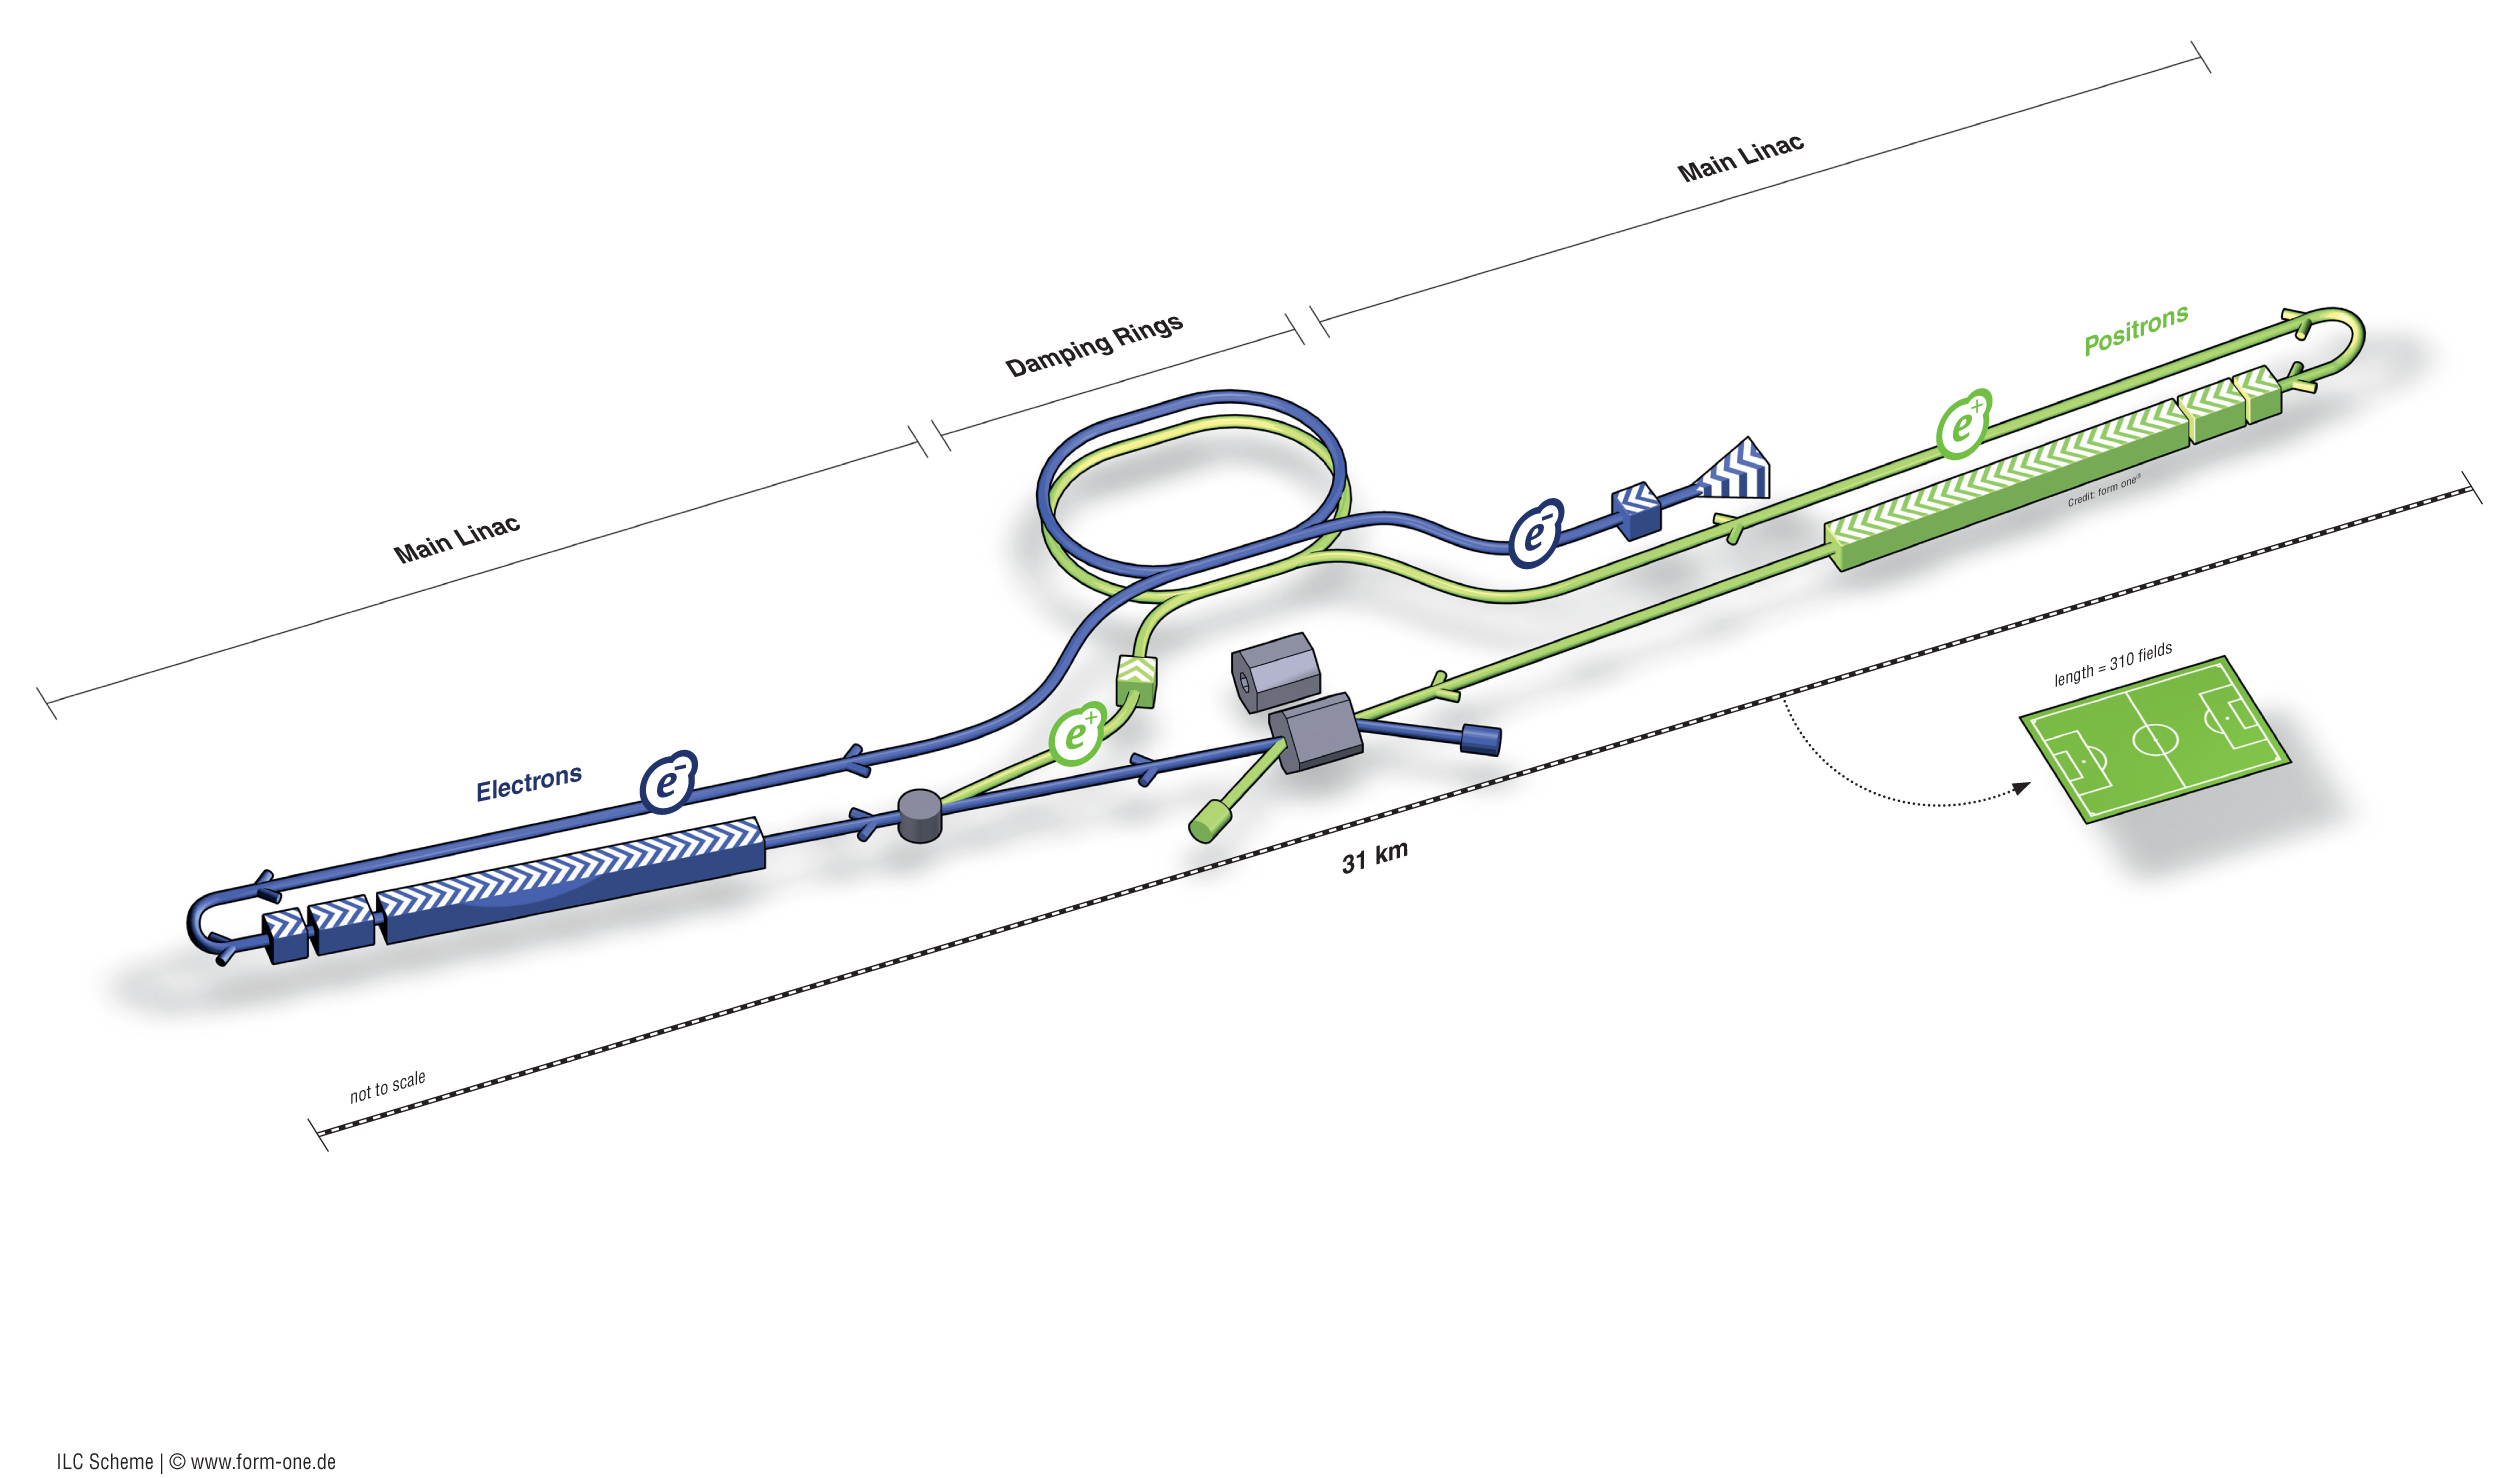
\includegraphics[width=0.9\textwidth,keepaspectratio]{Experiments/fig/ILC}
  \caption[The ILC Experiment]{The \ac{ILC} Collider\cite{ILCTDR}}
  \label{Fig:ILC}
\end{figure}

\subsection{Energy Staging}

The \ac{ILC} will first be built with a maximum collision energy capability of 500 GeV but with the potential for a later upgrade to 1 TeV which would require doubling the length of the machine to 62 km. The decision of whether the 1 TeV upgrade is necessary will largely be determined by the results of the \ac{LHC} experiments; if any new physics is discovered above 500 GeV then the 1 TeV upgrade could be essential to characterise it. Assuming the 1 TeV upgrade is realised the energy staging will be as described below.

The first three years will involve the ILC running at an energy of 250 GeV and taking 250 fb${^{-1}}$ of data. The main aim at this stage will be to measure the Higgs mass and ZH cross section from the Higgsstrahlung process as described in Chapter \ref{theory} to allow model independent measurements of the Higgs couplings to be performed.

For the following three years, the collider will then run at 500 GeV and will accrue a further 500 fb${^{-1}}$ of data. The main aims here will be to measure the HWW coupling, the total Higgs width and the absolute Higgs couplings to fermions. At this energy, measurements of top physics will also be possible including the top forward backward asymmetry. Outside of the Higgs sector, the top quark is perhaps the least well measured of the standard model particles and so provides another area in which to look for deviations from the standard model predictions.

After this there will be an upgrade to 1 TeV followed by another three years of data taking accumulating 1000 fb${^{-1}}$ of data. The aim of running at this high energy will be to search for new particles such as dark matter candidates and supersymmetric particles while improving upn the precision of the measurements performed at the lower energies. If one of these (or something entirely new) has already been discovered at the \ac{LHC} then the choice of 1 TeV might be scaled to match the scale of the newly discovered physics.

After this the collider will undergo a high luminosity upgrade and will run at the same energies for the same time periods for another 9 years but instead accruing 900, 1100 and 1500 ${fb^{-1}}$ at the respective energies. This will allow for a further increase in the precision of all measurements taken during the lower luminosity run.
While the \ac{TDR} proposes the above run scheme for the \ac{ILC} there is still debate about what energies should be used with arguments being made for running at 90 GeV (the Z mass) to gain precision measurements of the Z boson, 350 GeV (the top production threshold) to better measure the properties of the top quark or to simply only run at 250 GeV to provide precision Higgs measurements for minimal cost.

\subsection{Beam Production, Acceleration and Focusing}
\label{ILC:BEAM}

\begin{figure}
  \centering
  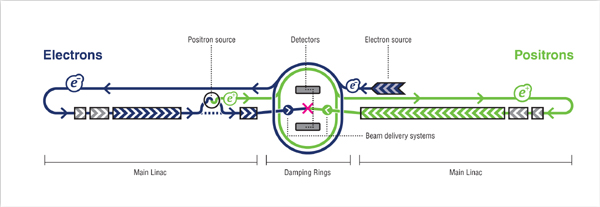
\includegraphics[width=0.9\textwidth,keepaspectratio]{Experiments/fig/ILC_Simplified}
  \caption[Schematic of the ILC accelerator layout]{A simplified schematic of the ILC\cite{ILCTDR}}
  \label{Fig:ILCsimple}
\end{figure}

\begin{table}
\caption[ILC Beam Parameters]{ILC Beam Parameters}
\label{table:ilcbeamparameters}
\centering
\begin{tabular}{l l l l l }
\toprule
\textbf{Parameter}                  & \textbf{Symbol}         & \textbf{Unit}& \textbf{Stage 1} & \textbf{Stage 2} \\
\midrule
Centre-of-mass energy               & $\sqrt{s}$                &GeV                                        & 250 & 500 \\
Repetition frequency                & $f_{\text{rep}}$        &Hz                                         & 5 & 5 \\
Number of bunches per train         & $n_{b}$                 &                                           & 1312 & 1312 \\
Number of particles per bunch                    & $N$                     &$10^{10}$                      & 2.0 & 2.0 \\
Bunch separation                    & $\Delta t_b$             &ns                                         & 554 & 554 \\
\midrule
Accelerating gradient               & $G$                     &MV/m                                       & 14.7 & 31.5 \\
Electron Polarization               & $P_-$                   &\%                                       & 80 & 80 \\
Positron Polarization               & $P_+$                   &\%                                       & 30 & 30 \\
\midrule
Total luminosity                    & $\mathcal{L}$           &$10^{34}\;\text{cm}^{-2}\text{s}^{-1}$     & 0.75 & 1.8 \\
Luminosity above 99\% of $\sqrt{s}$   & $\mathcal{L}_{0.01}/\mathcal{L}$    &                            & 87.1\% & 58.3\% \\
\midrule
IP RMS beam size                    & $\sigma_x/\sigma_y$     &nm                                         & 729.0/7.7 & 474/5.9 \\
RMS Bunch length                    & $\sigma_z$              &mm                                  & 0.3 & 0.3 \\
Horizontal emittance                & $\epsilon_x$            &$\mu$m                                     & 10  & 10 \\
Vertical emittance                  & $\epsilon_y$            &nm                                         & 35 & 35 \\
Estimated power consumption         & $P_{AC}$                &MW                                & 122    & 163   \\
\bottomrule
\end{tabular}
\end{table}

A simplified schematic of the \ac{ILC} accelerating structure is shown above in \reffig{Fig:ILCsimple} while a summary of the key beam parameters is shown in \reftab{table:ilcbeamparameters}. The first stage of the acceleration process is the production of electrons. This is done using the photoelectric effect by firing photons onto a GaAs target to produce photoelectrons. These electrons then enter a 3.2 km long damping ring which accelerates the beam up to 15 GeV. The primary purpose of the damping ring is to produce a homogeneous beam of electrons with uniform energy and momentum. After the damping ring the electrons enter into a two stage bunch compressor which separates the electron beam into ${\sim}$1300 bunches, each containing ${2\times10^{10}}$ electrons, with each bunch being separated by 554 ns and a maximum beam pulse length of $\sim$ 1.6 ms. The overall intended collision rate of these pulses is 5 Hz, which means that the duration for collisions is less than 1\% of the collision rate. This has important consequences for the detector design as it means the detectors have a large period of time in which to relax after events. As the detectors do not need to be operating for 99\% of the time, it is considerably easier to cool them meaning the material budget for the cooling systems within them can be greatly reduced. Following the bunch compression the electrons enter the main 11 km linac where they are accelerated up to the nominal beam energy using 7,400 1.3 GHz superconducting niobium \ac{RF} cavities (see \reffig{Fig:cavity}). 

\begin{figure}
  \centering
  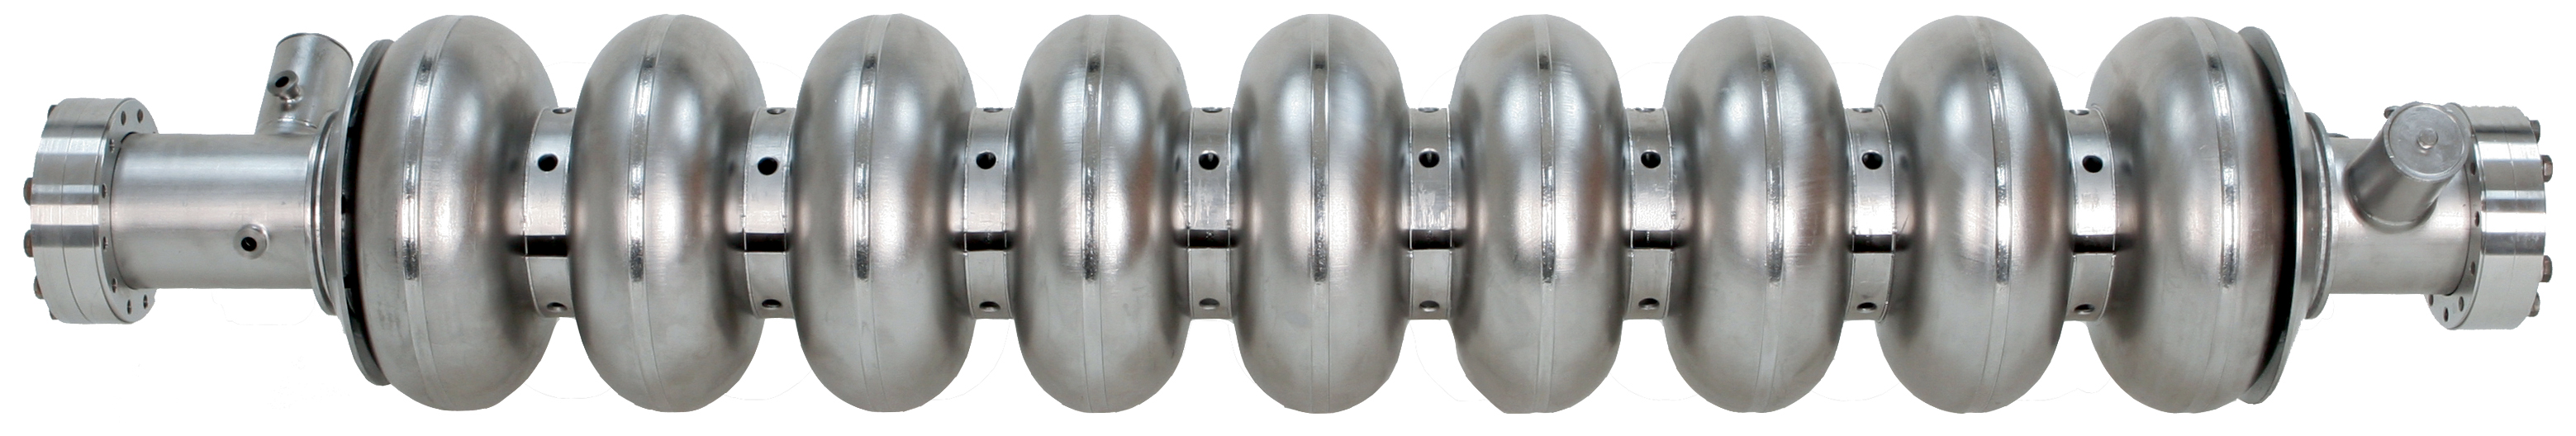
\includegraphics[width=0.75\textwidth,height=10cm,keepaspectratio]{Experiments/fig/Cavity}
  \caption[Superconducting Cavities For The ILC]{A 1.3GHz Superconducting Niobium Radio Frequency Cavity \cite{ILCTDR}}
  \label{Fig:cavity}
\end{figure}

The \ac{RF} cavities are kept at a temperature of 2K and act to produce an average accelerating gradient of up to 31.5MV/m (14.7MV/m for the 250GeV stage.)  The final stage before the collision is the \ac{BDS} which primarily acts to compress the beam into a ribbon shape with a cross-section of 7.7 x 729.0 nm while also handling the beam monitoring. The ribbon shape is designed to reduce \ac{BS} radiation from beam interactions while giving a small enough cross section that a high instantaneous luminosity can be achieved. Following the \ac{BDS} the beam finally enters the detector and collides with the oppposing positron beam at a crossing angle of 14 mrad then exits into the beam dump system which quenches what is left of the beam.

\subsection{Positron Production}
Positrons are produced at the \ac{ILC} by tapping off energy from the electron beam after it has been accelerated by the main linac. The electron beam is passed through an undulator which causes the electrons to emit synchrotron radiation in the form of 10-30 MeV photons by forcing the beam to take a rapidly varying path in the plane transverse to it's direction of motion. The resulting photons are then separated from the electron beam and are collided with a Titanium alloy target to produce electron positron pairs. The electrons and positrons are then separated and the electrons are dumped while the positrons are then passed into a damping ring and undergo all the same stages of acceleration and shaping as described above for the electrons.

\section{CLIC}

\begin{figure}
  \centering
  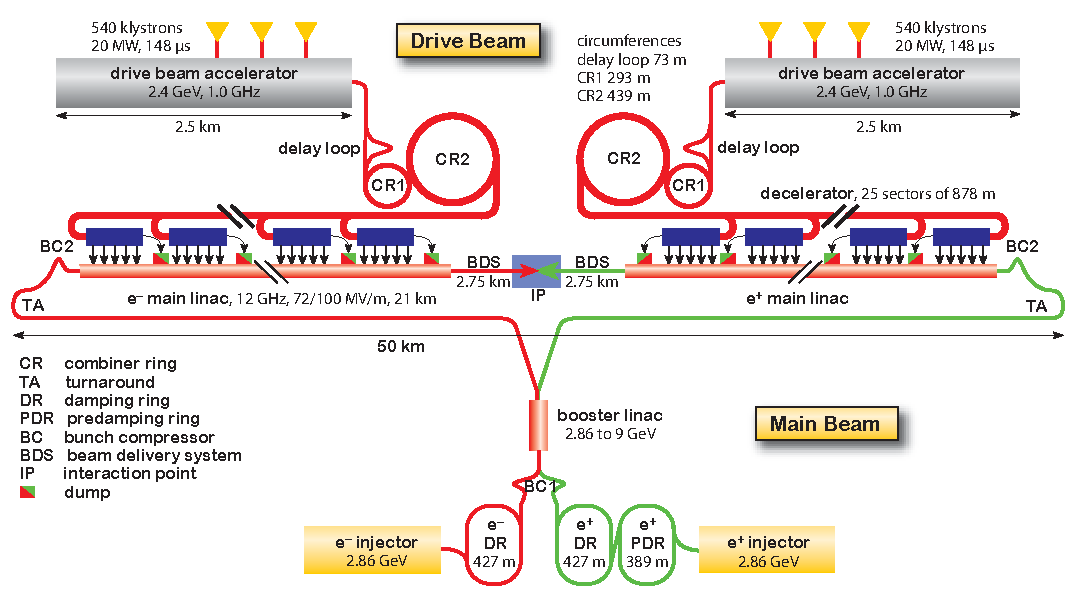
\includegraphics[width=0.75\textwidth,height=10cm,keepaspectratio]{Experiments/fig/CLIC-layout-3TeV}
  \caption[The CLIC Experiment]{The CLIC Collider. Layout for the CLIC accelerator at 3 TeV. For the lowest energy stage there will only be one drive beam constructed which will power both main beams\cite{CDR}}
  \label{Fig:CLIC}
\end{figure}

\begin{table}
\caption[CLIC beam parameters]{Parameters for the CLIC energy stages. The power consumptions for the 1.5 and 3\,TeV stages are from the CDR; depending on the details of the upgrade they can change at the percent level \cite{CLIC:2016zwp}.}
\label{table:clicbeamparameters}
\centering
\begin{tabular}{l l l l l l}
\toprule
\textbf{Parameter}                  & \textbf{Symbol}         & \textbf{Unit}& \textbf{Stage 1} & \textbf{Stage 2} & \textbf{Stage 3} \\
\midrule
Centre-of-mass energy               & $\sqrt{s}$                &GeV                                        & 380 & 1500 & 3000\\
Repetition frequency                & $f_{\text{rep}}$        &Hz                                         & 50 & 50 & 50\\
Number of bunches per train         & $n_{b}$                 &                                           & 352 & 312 & 312\\
Bunch separation                    & $\Delta\,t$             &ns                                         & 0.5 & 0.5 & 0.5\\
Pulse length                        & $\tau_{\text{RF}}$      &ns                                         &244 &244 &244\\
\midrule
Accelerating gradient               & $G$                     &MV/m                                       & 72 & 72/100 & 72/100\\
\midrule
Total luminosity                    & $\mathcal{L}$           &$10^{34}\;\text{cm}^{-2}\text{s}^{-1}$     & 1.5 & 3.7 & 5.9 \\
Luminosity above 99\% of $\sqrt{s}$   & $\mathcal{L}_{0.01}$    &$10^{34}\;\text{cm}^{-2}\text{s}^{-1}$     & 0.9 & 1.4 & 2\\
\midrule
Main tunnel length                  &                         &km                                         & 11.4 & 29.0 & 50.1\\
Number of particles per bunch                    & $N$                     &$10^9$                                     & 5.2 & 3.7 & 3.7\\
Bunch length                        & $\sigma_z$              &$\mu m$                                  & 70 & 44 & 44\\
IP beam size                        & $\sigma_x/\sigma_y$     &nm                                         & 149/2.9 & $\sim$ 60/1.5 & $\sim$ 40/1\\
Normalised emittance (end of linac) & $\epsilon_x/\epsilon_y$ &nm                                         & 920/20 & 660/20 & 660/20\\
Normalised emittance (at IP)        & $\epsilon_x/\epsilon_y$ &nm                                         & 950/30 & ---    &---\\
Estimated power consumption                        & $P_{\text{wall}}$         &MW                                & 252    & 364    & 589\\
\bottomrule
\end{tabular}
\end{table}

\ac{CLIC} is an experiment based at CERN which proposes the building of a 42 km accelerator at the main CERN site in Geneva (\reffig{Fig:CLIC}.) Despite being named as “compact”, \ac{CLIC} is actually longer than the initial 500 GeV \ac{ILC}. The reason for this naming is that \ac{CLIC} has a much higher accelerating gradient (100 MeV/m) compared to ILC and so provides a much higher energy per length. The expected build date for \ac{CLIC} is still relatively uncertain though is likely to be no earlier than 2030 as the accelerating technology required for \ac{CLIC} is less developed than that used by \ac{ILC}. This difference in the maturity of the two experiments can be seen from the fact that the \ac{ILC} has released its \ac{TDR} while the most comprehensive document for the CLIC project is still its \ac{CDR} \cite{CDR}. Updates on this document have been provided in the New Baseline Report \cite{CLIC:2016zwp} released in 2016 and any details specified here can be assumed to come from these two documents. 

Overall the design for \ac{CLIC} is relatively similar in layout to the \ac{ILC} but with a few changes. Positron production at \ac{CLIC} is done completely independently from the main electron beam, though they are still produced via the same mechanism as before. The \ac{BDS} still compresses the beam into a ribbon shape to give it a small cross-section and reduced \ac{BS}, however the aspect ratio is reduced compared to at \ac{ILC}. This results in larger contributions from beam photon radiations at \ac{CLIC}. The collision rate at \ac{CLIC} is significantly higher as it aims to be a high luminosity device- the collision rate will be 50 Hz with 354 bunches per pulse with a separation of just 0.5 ns. This means that CLIC will have a significantly higher duty cycle which will make cooling of the detectors harder and will give the detectors less time to relax after events. A summary of the beam parameters for CLIC is shown in \reftab{table:clicbeamparameters}. While these difference are important, the most significant changes are in the energy staging and acceleration technology used at \ac{CLIC} (see \refsec{sect:clicaccelerator}.)

\subsection{Energy Staging}

CLIC will operate at three energy stages- 380 GeV, 1.5 TeV and 3 TeV collecting 500 ${fb^{-1}}$, 1.5 ${ab^{-1}}$ and 2 ${ab^{-1}}$ of data respectively. During the running of the 380~GeV energy stage, construction of the 1.5~TeV structure will be carried out (and so on for the 1.5 TeV and 3 TeV scales) so as to reduce the delay between operation at successive energy stages. 

The 380 GeV energy scale is chosen as it is above the \ttbar production threshold and provides a significant cross section for many channels involving the top quark. This stage is also supplemented by a series of 10 measurements around the \ttbar threshold taking 10 ${fb^{-1}}$ each with the aim of measuring the top mass and width from the line shape of the \ttbar production cross section at threshold. The 380~GeV stage will also be used to provide measurements of the higgs boson similar to those performed at \ac{ILC} during it's two lower energy stages.

The 1.5 TeV energy stage provides the ability to further study the top and higgs in more detail with several new channels becoming significant e.g top yukawaw coupling, higgs self coupling, while the 3~TeV stage pushes the energy frontier allowing the possibility of direct detection of new physics at the multi-TeV scale. The choice of 3~TeV is based upon certain models of supersymmetry which predict new particles to exist at this energy (see \reffig{Fig:SuperSym}).

For clarification it should be stated that for many years the proposed scheme for CLIC was actually to operate at 500~GeV, 1.4~TeV and 3~TeV. These were updated to provide better precision on measurements of the top quark during the lowest energy stage (\ttbar production threshold is $\sim$ 350 GeV) and improved precision on the Higgs self-coupling during the second stage. It is important to be aware of these changes as the studies presented in chapters \ref{Higgs Analysis} and \ref{chapter:topanalysis} were both carried out at 1.4 TeV assuming the original energy staging, however it is expected that there will be negligible impact on the findings of these studies from changing the energy to 1.5 TeV.  

\begin{figure}
  \centering
  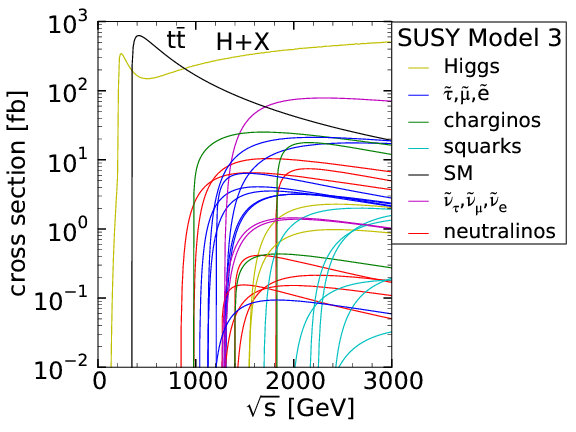
\includegraphics[width=0.75\textwidth,height=10cm,keepaspectratio]{Experiments/fig/clicSS}
  \caption[Cross Sections For Supersymmetric Processes at \ac{CLIC}]{Cross sections for production of various supersymmetric particles at an ${e^+e^-}$ collider as a function of centre of mass energy.}
  \label{Fig:SuperSym}
\end{figure}

\subsection{Acceleration Technology}
\label{sect:clicaccelerator}
Unlike \ac{ILC}, the acceleration technology will not be superconducting but will instead use two beams of electrons-- referred to as the main beam and the drive beam-- rather than just one main accelerated beam. The drive beam is accelerated using standard accelerating technology (klystrons) as in \ac{ILC} to accelerate bunches of electrons to 2.75 GeV. These bunches then enter a series of delay/control rings which are designed such that the electrons within them get combined with the new electrons being added from the drive beam accelerator to build up a large number of low energy electrons which combined carry a large amount of energy. The energy from this beam is then used to drive the main beam. This is done by rapidly decelerating the drive beam electrons down to 10\% of their initial energy and using the resulting \ac{RF} produced to accelerate the smaller number of electrons in the main beam resulting in a rapid acceleration. The main beam is then used to supply collisions. Overall the result is that the machine is simply acting as a novel form of transformer, converting a high current, low energy beam of electrons into a lower current, high energy beam. This approach allows for very high accelerating gradients but has the disadvantage that in approximately 1\% of events the sudden input of energy from the drive beam can cause electrical breakdowns in the main beam cavity, which disrupt the alignment and structure of the main beam making them unsuitable for use.

\section{Linear Collider Analysis Framework}

A common framework known as ILCSoft used for event simulation, reconstruction and analysis has been developed for both \ac{ILC} and \ac{CLIC} to allow for sharing of techniques between the two experiments. Here we will provide an overview of the key packages used.

\subsection{Event Generation}

Event generation is performed using an external package called WHIZARD \cite{Kilian:2007gr}. WHIZARD itself handles most of the event generation such as the calculation of hard matrix elements, phase space considerations and accounting for interference between processes, however for certain aspects it relies on additional packages. The most relevant of these are tau decays which are handed by TAUOLA\cite{Jadach:1990mz} and hadronization which is handled by PYTHIA\cite{Sjostrand:2006za}. Unfortunately no other hadronization package is available within WHIZARD which makes it challenging for evaluating systematic uncertainties arrising from how jets are modelled. The output from WHIZARD is a series of four momenta for all the particles produced in the collisions. These are then passed to a package called MOKKA whcih acts as an interface to GEANT4\cite{MoradeFreitas:2002kj}. Within MOKKA the interaction of the particles with the detector is modelled and a series of energy deposits are recorded for the various subdetector components. These are then finally passed on to the ILCSoft reconstruction package MARLIN in which digitisation of the hits and track reconstruction occur to produce realistic outputs from the detector. At this stage $\gamma\gamma\rightarrow$ hadron beam backgrounds are overlayed on the events assuming a rate of 1.6 events per bunch crossing.


\subsection{Pandora Particle Flow Algorithm}
\label{Pandora}

Pandora\cite{Thomson200925} is an advanced Particle Flow Algorithm used at linear colliders which allows an increased level of precision from detector measurements. The underlying principle behind particle flow is to try and always use the most precise detector component for performing energy measurements where possible. Typical values for energy resolutions for a charged particle in the main detector components are 10$^{-4} \times$ $E^2$ in the tracker, 0.15 $\times \sqrt{E}$ in the \ac{ECAL} and 0.55 $\times \sqrt{E}$ in the \ac{HCAL}. For a typical jet the composition will usually be $\sim$60\% charged hadrons, 30\% photons and 10\% hadrons. Traditionally for measuring the energy in a jet one would simply sum the deposits in both calorimeters resulting in a relatively poor energy resolution of $\sim$60\%/$\sqrt{E}$ due to the large component being measured in the \ac{HCAL}. If one can measure the charge hadron component in the tracker instead, this performance can be vastly improved to $\sim$20\%/$\sqrt{E}$. In order to be able to reach this performance, accurate association of tracks with deposits in the calorimeters is crucial. This is achieved by having a high granularity calorimeter and a high spatial resolution for the tracker. In practice however, even with a well designed detector, the particle flow algorithm can still fail to reconstruct the correct energy due to ambiguities referred to as ``confusion''. For example, if a photon enters the calorimeter near to a charged hadron, it is possible that the two will not be resolved and the energy identified from just using the track will neglect the contribution from the photon. Energy can also be overestimated in cases where a charged hadron showers in such a way that it looks like two separate calorimeter deposits which results in part of the shower being identified as a neutral hadron and the other fragment being associated with the track. One of the main design aims of the detectors will be to try and minimise these confusion effects. 


\section{Detectors}
The \ac{ILC} has been designed with the intention of having two unique detectors so that results can be validated by cross-checking between the two detectors. However, because \ac{ILC} is a linear collider it is only feasible to have one interaction point and as a result the beam time will have to be shared between the detectors. This will be done using a 'push-pull' design in which both detectors are placed on a single platform at the interaction point which can be moved back and forth to position the desired detector in the path of the beams. While having two detectors is certainly desirable as it allows the gathering of two independent sets of results for the collider and allows the continued taking of results when one of the detectors requires maintenance, it also has disadvantages as it means an increase in the dead time of the machine (as swapping the detectors is a slow process taking several days which will be done multiple times a year) and an increase in the cost of the experiment. As a result the possibility of using only one detector is still being considered as a potential option. The possibility of splitting the main beam and having two IPs is also being proposed so that both detectors could be used simultaneously however this would be expensive as extra tunnels would have to be built to accomodate this and there would also be a reduction in the beam quality as splitting the beam would produce synchotron radiation. The studies presented in this thesis are based on simulations of only one of these detectors, \ac{ILD}\cite{ILD}, and as such we will not give details of the alternative: \ac{SiD}\cite{Aihara:2009ad}. 

\subsection{ILD}
\begin{figure}
  \centering
  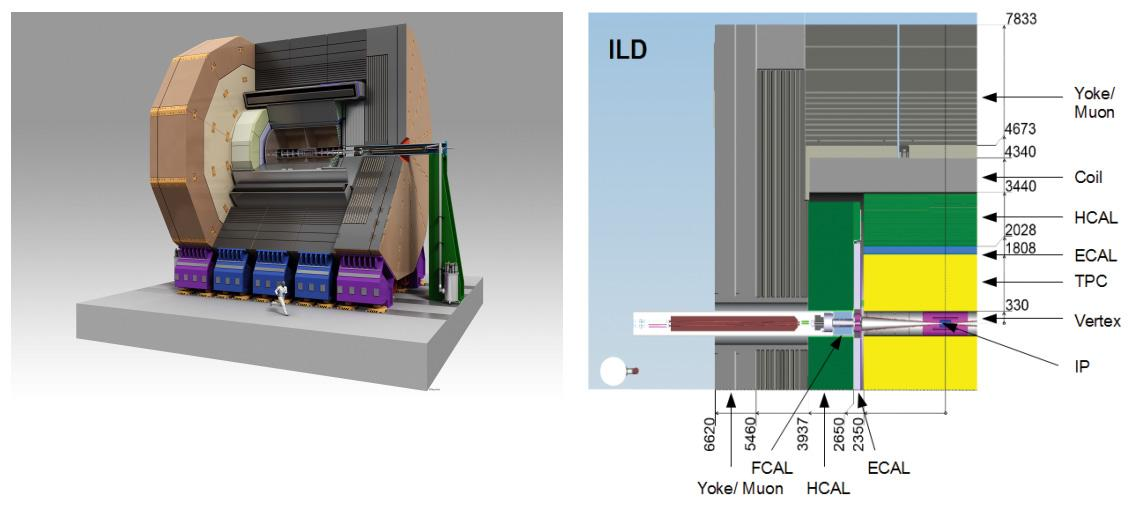
\includegraphics[width=0.95\textwidth,keepaspectratio]{Experiments/fig/ILD}
  \caption[ILD Detector]{The International Large Detector Concept (left). Schematic of the ILD showing the key components in a one-quarter view of a vertical section of the detector (right). Dimensions ar in mm \cite{Behnke:2013xla}}
  \label{Fig:ILD}
\end{figure}

The ILD (shown in \reffig{Fig:ILD}) is a general purpose detector which is cylindrical in design with radius 8m and length 14m. The different sub-detectors are arranged in a concentric manner in the main barrel of the detector, and are positioned with the vertexing technology closest to the beamline, followed by trackers, then electromagnetic and hadronic calorimeters, then the magnetic field coils which supply a 3.5T B-field and finally muon tail catchers. The detector has two endcaps with a similar layer structure at each end of the barrel creating a hermetic seal.

In order to provide precision measurements of the various processes proposed in the \ac{ILC} and \ac{CLIC} physics schemes, there are several strict requirements imposed upon the performance of the detector:

\begin{itemize}

\item \textbf{Momentum Resolution}: $\sigma_{p_t}^2/ p_{t}^2 \sim 2 \times 10^{-5} GeV^{-1}$, key for precision Higgs recoil mass measurements

\item \textbf{Jet Energy Resolution}: $\sigma_E/E \sim 3-4\%$, allows separation of hadronic W/Z decays

\item \textbf{Impact Parameter Resolution}: $\sigma_{b} < 5 \oplus \frac{10}{p\sin\theta^{\frac{3}{2}}}\mu m$, allows accurate flavour tagging for short lived particles

\item \textbf{Hermetic Coverage}: Needed for processes with a strong angular dependence or missing energy component 

\end{itemize}

Detailed specifications for the detector can be found in the \ac{ILD} Letter of Intent \cite{ILD}. Here we will give a brief overview of the key components, their functions, and the methods used for making the most of the information they provide.

\subsubsection{Vertexing}

The vertexing technology is used to gain information about heavier particles such as b-quarks which have very short lifetimes ($\sim$10$^{-12}$s) and so decay close to the beamline before they can reach the trackers or calorimeters. As such, the vertexers are placed extremely close to the beamline and work by looking for displaced vertices from the initial \ac{IP} which correspond to the point at which the heavy flavour paricles decayed. Due to their proximity to the beam line it is always necessary for the vertex detectors to be radiation hard as they are exposed to stray high energy particles from the beam. The vertexers also act as trackers for short lived particles that fail to reach the main trackers and so are required to be highly granular to separate particles that have had very little time to spread out since the \ac{IP}. The design for the vertex detectors is yet to be finalised as there are numerous competing technologies under consideration, but the target performance is to achieve a track impact parameter resolution of

\begin{equation}
\sigma_{b} < 5 \oplus \frac{10}{p\sin\theta^{\frac{3}{2}}}\mu m
\end{equation}

where $p$ is the track momentum in GeV, $\theta$ is the angle between the track and the vertex detector plane and the first and second terms describe contributions from the transverse impact parameter resolution and multiple scattering effects respectively.  In practice it is found that to achieve this impact parameter resolution a spatial resolution of at least 3 $\mu m$ is required. As well as achieving a sufficienct impact parameter resolution, the vertexing detectors are also required to have sufficient granularity and low enough occupancy rates to allow separation of individual tracks passing through the detector. On top of these requirements for the vertexing and tracking performance, the design for the vertexer must also avoid any negative impact on later parts of the detector. In particlular, the material budget of the whole detector system is limited to be less than one radiation length to avoid unwanted production of electromagnetic showers prior to the \ac{ECAL}. The detector layout used for the baseline studies in the \ac{ILD} \ac{TDR} assumes six layers of 50$\mu m$ thin silicon pixels arranged in pairs. The layout and details of the structure are shown in more detail in \reffig{fig:VTX} and \reftab{tab:aVTX}.

\begin{figure}
  \centering
  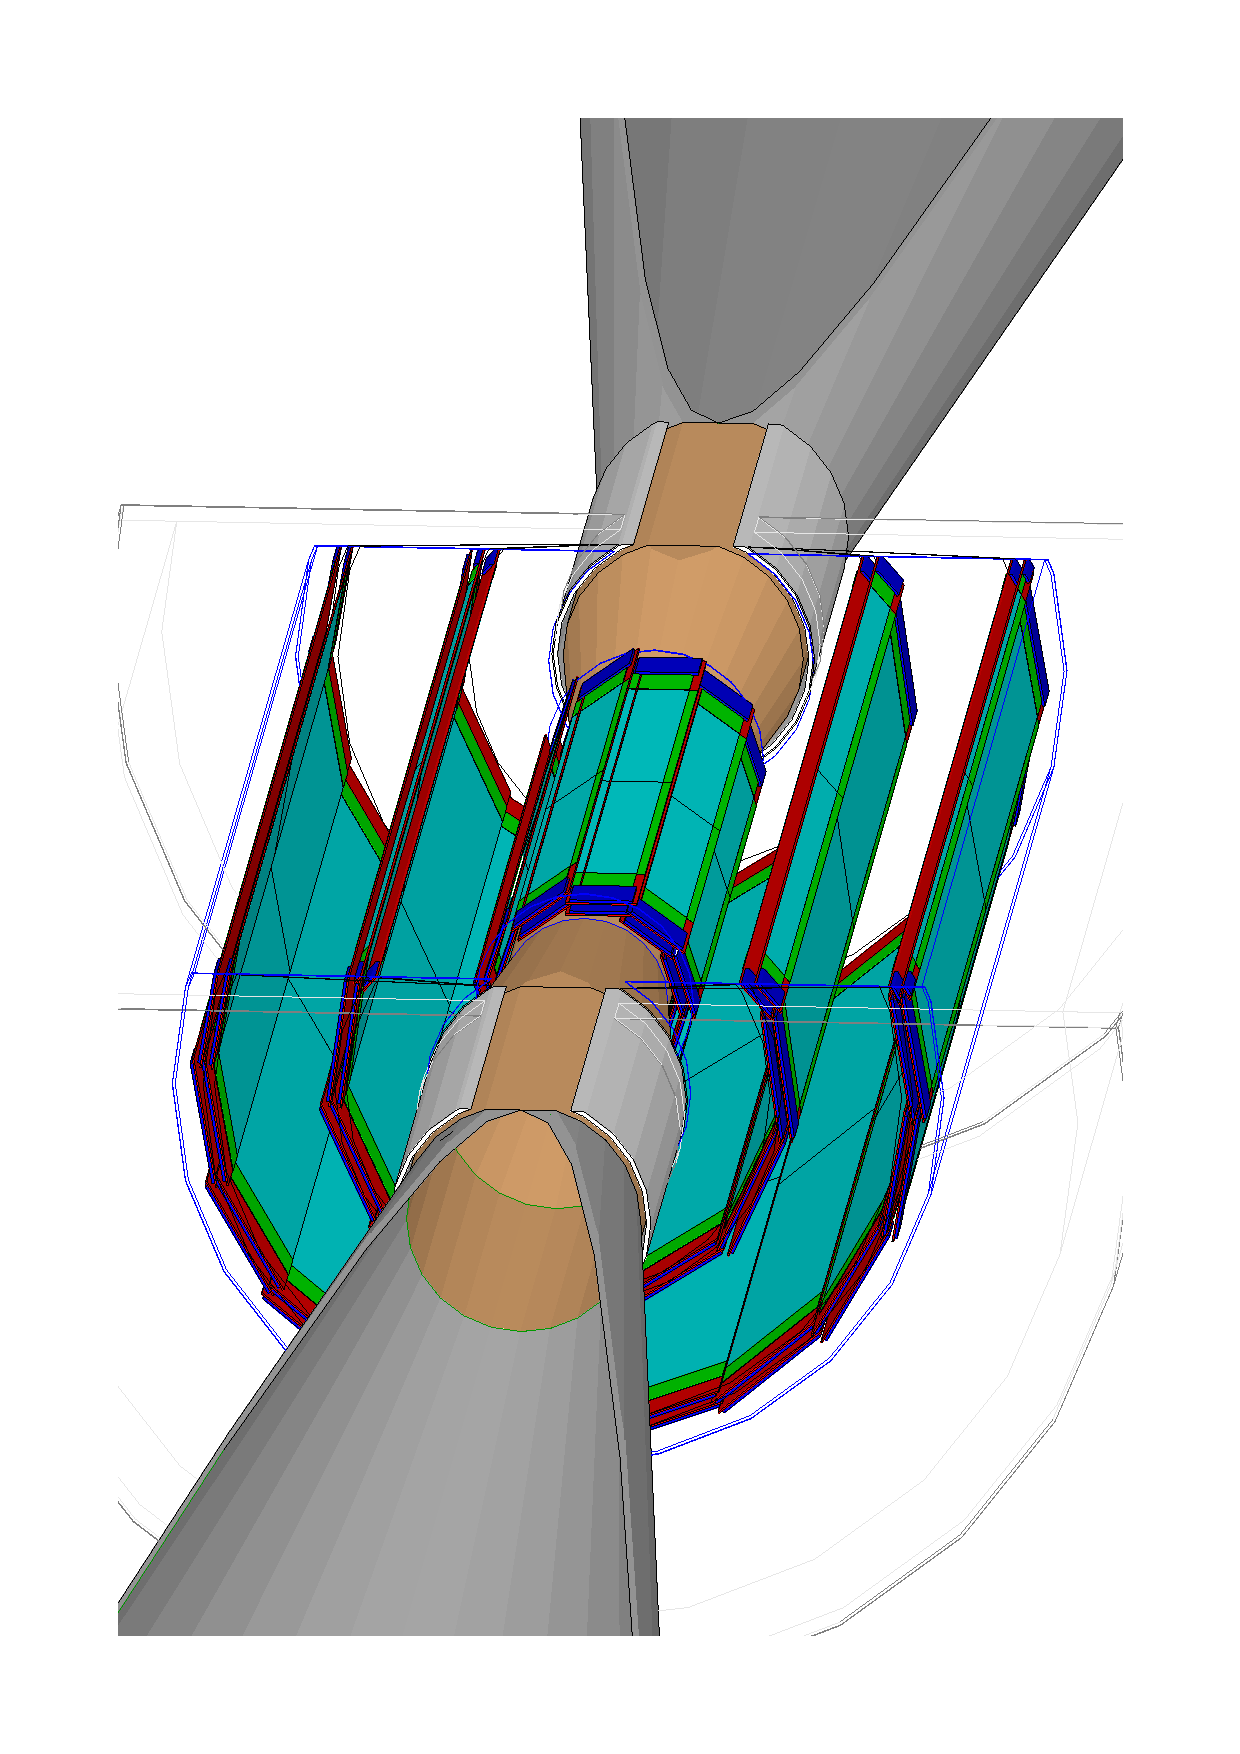
\includegraphics[width=0.3\textwidth,keepaspectratio]{Experiments/fig/Vertex}
  \caption[ILD Vertex Detector]{Proposed vertex detector geometry for ILD \cite{ILD}}
  \label{fig:VTX}
\end{figure}

\begin{table}
  \caption{Properties of the CLIC vertex detector assuming three pairs of layers \cite{ILD}}
  \centering

  \begin{tabular}{l l l l l l l}
    \toprule
    layer           & radius [mm]         & ladder length [mm]  & read-out time [$\mu s$]  \\
    \midrule
    1 & 16.0 & 125.0 & 25-50 \\
    2 & 18.0 & 125.0 & 25-50 \\
    3 & 37.0 & 250.0 & 100-200 \\
    4 & 39.0 & 250.0 & 100-200 \\
    5 & 58.0 & 250.0 & 100-200 \\
    6 & 60.0 & 250.0 & 100-200 \\
    \bottomrule
  \end{tabular}
  \label{tab:aVTX}

\end{table}


\subsubsection{Tracking}

Tracking in \ac{ILD} is performed by multiple subsystems. We have already discussed the vertexing systems which act as trackers for low transverse momentum and short lived particles, however the majority of the tracking is performed by a large \ac{TPC}.  This is a large gas filled cylinder extending from r=395 mm to r=1739mm with an electric field applied across it and readout electronics at each end of the cylinder on the endcaps. As particles pass through the gas, they ionize it producing charged particles. The electric field then causes these particles to drift to each end of the detector where they are collected by the electronics. By measuring the position and time at which the charged particles arrive, the track of the original ionizing particle can be reconstructed. A magnetic field is also generated across the chamber to deflect the charged particles so that the momentum and charge of the particle can be estimated. The magnetic field used in the ILD is a 3.5T coil placed outside the calorimeters to minimize the material budget in front of the calorimeters. The use of a \ac{TPC} provides several benefits over alternative technologies such as silicon tracking (the technology used in the \ac{SiD} tracker.) Because the ionization occurs across the whole track, it is possible to reconstruct the particles path from numerous spacial points to provide a precise meaurement of the path taken. This is not the case for a silicon tracker where the number of data points is proportional to the number of tracking layers present, however this is compensated for by the fact silicon trackers typically have a higher spatial resolution on each point ($\sim 1~\mu m$) compared to TPCs ($\sim 1~mm$.) TPCs also benefit from having a low material budget compared to silicon trackers. In \ac{ILD} the gas used will be Ar:CH$_{4}$:CO$_{2}$ (95:3:2) which gives a material budget of $\sim 0.04(0.15)X_0$ radially(longitudinally.) The choice of readout technology is yet to be finalised with several options being pursued (Micro-Pattern Gas Detectors, MicroMegas\cite{Giomataris:1995fq} and GEM\cite{Sauli:1997qp}) however in all cases it is expected that there will be 10${^{-6}}$ channels of diminsion $\sim$1$\times$6 mm$^{2}$. This system will allow a single point resolution of $<$100$~\mum$(0.5 mm) and two hit resolution of 2 mm (6 mm)  in the x-y (r-z) planes, and a resolution of 5$\%$ on dE/dx.

The \ac{TPC} is supplemented by a series of silicon based tracking systems whcih act to provide high spatial resolution points at the entrance and exit of the TPC which yields an improved momentum resolution and an improved performance from the \ac{PFA}s, provide time stamping for bunch tagging and assist in calibration of the \ac{TPC}. These additional subdetector systems come in four parts. In the barrel region, between the vertexer and the \ac{TPC} lies the \ac{SIT} which provides two high spatial resolution points at r= 165 mm and r=309 mm, while between the \ac{TPC} and the \ac{ECAL} lies the \ac{SET} which provides a single spatial point at r=1844 mm. Both of these systems are based on double sided silicon microstrips and provide a resolution of $\sim$ 50 um. The \ac{FTD}covers the very forward region of the detector down to 0.15 radians and consists of 7 disks positioned in the innermost tracking region, the first three using silicon pixels and the end 4 using silicon microstrips. The \ac{ETD} is similar in structure to the \ac{SET} but is positioned outside the \ac{TPC} endcaps rather than the barrel to provide high spatial resolution for particles exiting the tracker into the endcap calorimeters. The positioning of all these subdetector systems can be seen in \reffig{fig:silicontracking}.

\begin{figure}
  \centering
  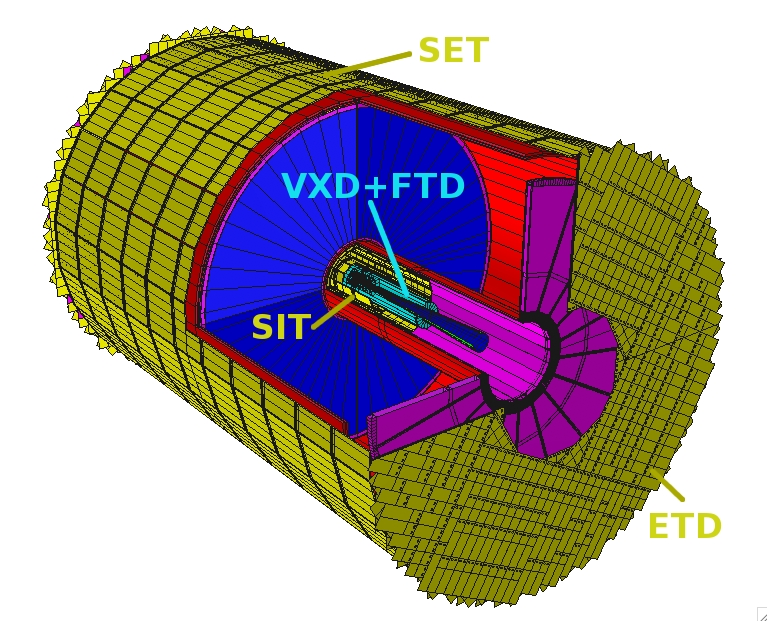
\includegraphics[width=0.5\textwidth,keepaspectratio]{Experiments/fig/SiliconTrackers}
  \caption[Silicon Tracking Systems For ILD]{Silicon Tracking Systems For ILD \cite{ILD}}
  \label{fig:silicontracking}
\end{figure}

The combined performance of the vertexer, \ac{TPC} and silicon tracking systems gives a momentum resolution of $\sigma_{p_t}^2/ p_{t}^2 < 2 \times 10^{-5} GeV^{-1}$ and a tracking coverage reaching to as low as $\cos\theta<$0.996.


\subsubsection{Calorimetry}
\label{det:ecal}
The function of calorimeters is to measure the energy of particles by passing them through a medium in which they will deposit some of their energy. As the way that particles interact with other matter is determined by the type of particle invloved, the calorimeters are usually split into two two sections, the \ac{ECAL} and \ac{HCAL}, that are designed to interact with electromagnetic particles (electron, photons) and hadrons respectively. As we will later be presenting work on a proposed novel design for a \ac{DECAL} it is pertinent to discuss in greater detail the relevant processes and terminology involved in electromagentic calorimetry to understand what issues there are with current \ac{ECAL} technologies and how the \ac{DECAL} might improve upon them.

When an electron interacts with matter it will typically radiate a photon via \ac{BS}. This photon then can then decay into an electron-positron pair which will in turn radiate further photons. This cascade process results in the formation of what is refered to as an electromagnetic shower. The shower will continue to develop until the energy of the shower particles reaches a critical value, E$_{C}$, at which the energy losses of the particle begin to be dominate by ionization rather than beamsstrahlung. The development of the electromagnetic shower can be characterised using several parameters. The most commonly used of these is the the radiation length, $\chi_0$, which is defined as the distance an electron can travel through a material before it's energy has reduced by a factor of 1/e via beamsstrahlung (or equivalently to 7/9 the mean free path for pair production of a photon.) The interaction length can be expressed as a function of a materials nuclear parameters \cite{Groom:1998it}:

\begin{equation}
  \chi_0= \frac{kA}{Z(Z+1)\ln{287/sqrt{Z}}}
\end{equation}

Where k is a constant equal to 716 gcm$^{-2}$, A is atomic mass, and Z is atomic number.

For the purposes of designing a detector, perhaps the most relevant parameters are those related to the size of the showers as these determine the dimensions required for the calorimeter to contain the shower. The longitudinal detector requirements are decided by the rate of energy loss for a particle which is given by the Bethe-Bloch equation which can be simplified to\cite{Beringer:1900zz}:

\begin{equation}
  \label{bethebloch}
\frac{dE}{dx}=E_0 b \frac{(bx)^{a-1}e^(-bx)}{\Gamma(a)}
\end{equation}

Where x is the material depth in units of $\chi_0$, $E_0$ is the initial energy of the particle, and a and b are properties of the absorbing material. The exponential term means that it is typically not possible to capture 100\% of the energy in a shower, instead an acceptable level of loss must be decided and the detector designed accordingly. For example, a typical energy scale for \ac{CLIC} would be $\sim$ 100 GeV. For a working point of 5\% loss a calorimeter depth of $\sim$17 $\chi_0$ is required, while for an improved performance of just 1\% loss a depth of $\sim$20 $\chi_0$. The transverse profile of the shower is described by the Moliere radius, the radius in which 90\% of a particles energy will be deposited:

\begin{equation}
R_M=\frac{21MeV}{E_c}\chi_0
\end{equation}

In general, it is necessary to have a Moliere radius that is smaller than the typical separation of particles produced in a collision so as to avoid overlapping of showers. For \ac{ILD} this is espeically true where Pandora \ac{PFA} relies on accurate association of tracks to calorimeter deposits which is only possible if the deposits from nearby particles can be distinguished.

For \ac{ILD} the \ac{ECAL} and \ac{HCAL} are both sampling calorimeters. This means that the structure is divided into layers of two alternating materials known as the absorber and active material. The absorber is typically a thick piece of high Z material that acts to initiate an \ac{EM} shower. The active material is then a thin low Z material that is easily ionizable and so acts to collect charge deposited from the shower. The active layer will then be instrumented to collect and readout the charge deposited within it. In order to reconstruct the energy of the initial particle that produced the shower, one would ideally just sum the deposits from each of the active layers, however in reality there will also be some energy deposited within the absorbing material that must be accounted for. This is done by scaling the energy deposited by the expected ratio of the energy deposited in the active layer to the total energy deposited in the active and absorbing layers combined. The scale factors will usually be determined as part of a calibration procedure for the detector in which muons are passed through each layer. The application of these scale factors introduces an uncertainty in the reconstructed energy as they represent an average scale correction, whereas the actual ratio of the energy deposited in the active and absorbing layers will be determined by additional factors that can't be easily measured. One example would be the path taken by the particle which can change the relative distance travelled by the particle in the active and absorbing layers.

The overall performance of a calorimeter is given by the energy resolution. This represents the quadrature sum of all sources of uncertainty in the energy reconstruction which are usually borken down by their energy dependence and expressed as follows:

\begin{equation}
  \frac{\sigma_E}{E}=\frac{a}{\sqrt{E}} \oplus \frac{b}{E} \oplus c
\end{equation}

Where a, b and c are typically referred to as the stochastic, noise and leakage terms. The energy dependence of the background and leakage terms are straightforward to understand. Noise typically arrises from the electronics used for collecting and reading out the hits in the active layers. This means that it is independent of the energy of the incident particles energy and so the absolute uncertainty doesn't vary with E. The leakage term accounts for the amount of energy lost from the calorimter not being deep enough to contain the shower. One can see from \refeq{bethebloch} that the energy lost will scale with the incident particles energy.

The stochastic term is slightly more complicated as it represents a combination of effects. The first of these is the intrinsic resolution of the detector which is determined by the physics of how an \ac{EM} shower develops. The number of particles produced in a shower (N)  is proportional to the energy of the incident particle (E), however the formation of bremstrahlung photons and electron-positron pairs is a quantum mechanical process and so is inherently statistical. As a result N will follow a Poisson distribution and so the uncertainty on it will be 1/$\sqrt{N}$. As N is proportional to E, this means there is an inherent uncertainty in the energy proportional to 1/$\sqrt{E}$. There are also further statistical contributions that arrise from using a sampling approach. For low energy particles produced in the absorber there is a chance that they be absorbed before making it to the active layer and so will not be accounted for in the scale factors. The uncertainty associated with this can be described by $\sqrt{E_{c}x/E}$. This factor is further added to by the effect mentioned above where x will vary from particle to particle depending on the path it takes through the detector. Because the energy deposited in a material as a function of the material depth is described by a landau distribution, uncertainties from varying path lengths are often referred to as landau fluctuations with the form $\sigma_{landau}/\sqrt{E}$.

\subsubsection{ECAL}
The \ac{ILD} \ac{ECAL} is a highly granular calorimeter poitioned at r=1847mm which consists of 30 active layers separated by layers of absorbing material. Tungsten is chosen for the absorber due to it's short radiation length, $\chi_0$=0.35cm. The first 20 absorber layers are 0.6$\chi_0$(2.1mm) thick while the later layers are  1.2$\chi_0$ to contain higher energy \ac{EM} showers while maintaining a compact design. The structure of the \ac{ECAL} is shown in \reffig{Fig:ECAL}. The active material will conisist of 5x5 mm$^2$ pitch silicon pixels and yields a resolution of

\begin{equation}
  \frac{\sigma_E}{E}=\frac{16.6\pm 0.1}{\sqrt{(E(GeV)}}\oplus(1.1\pm 0.1)\%
\end{equation}

While this is currently the default used in simulations for physics analyses, the choice of active material is yet to be finalised. A variation that uses 10x45 mm$^2$ silicon scintillator strips which would be rotated by 90${^o}$ in each successive layer to produce an effective cell size of 10x10 mm$^2$ with photomultipliers attached to each strip for readout also exists. The energy resolution for this form of the detector has been measured to be

\begin{equation}
  \frac{\sigma_E}{E}=\frac{14}{\sqrt{E}}\oplus2\%
\end{equation}

however the pixel version is typically favoured due to it's simpler design which doesn't require additional processing to produce the desired granularity.

\begin{figure}[h]
  \centering
  \begin{tabular}[c]{cc}
  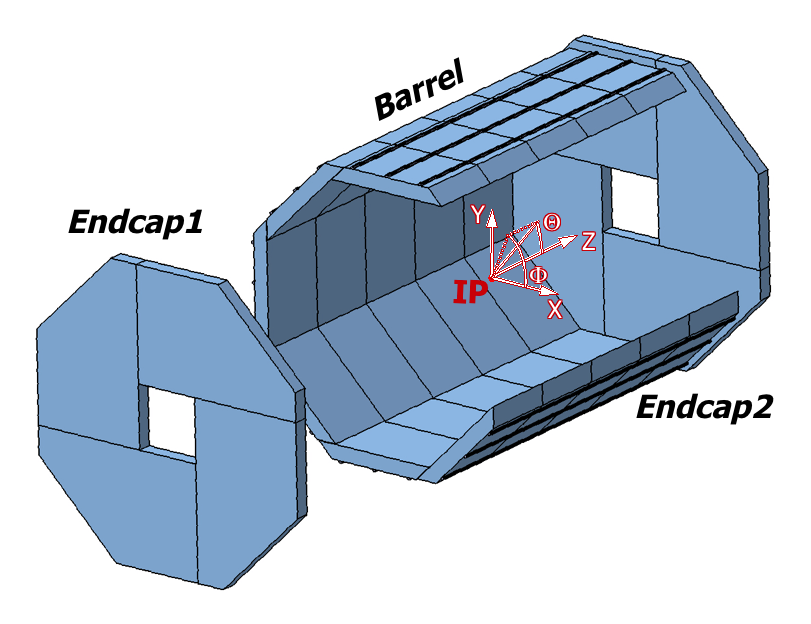
\includegraphics[height=5.5cm]{Experiments/fig/ECALview_global_annot} &
  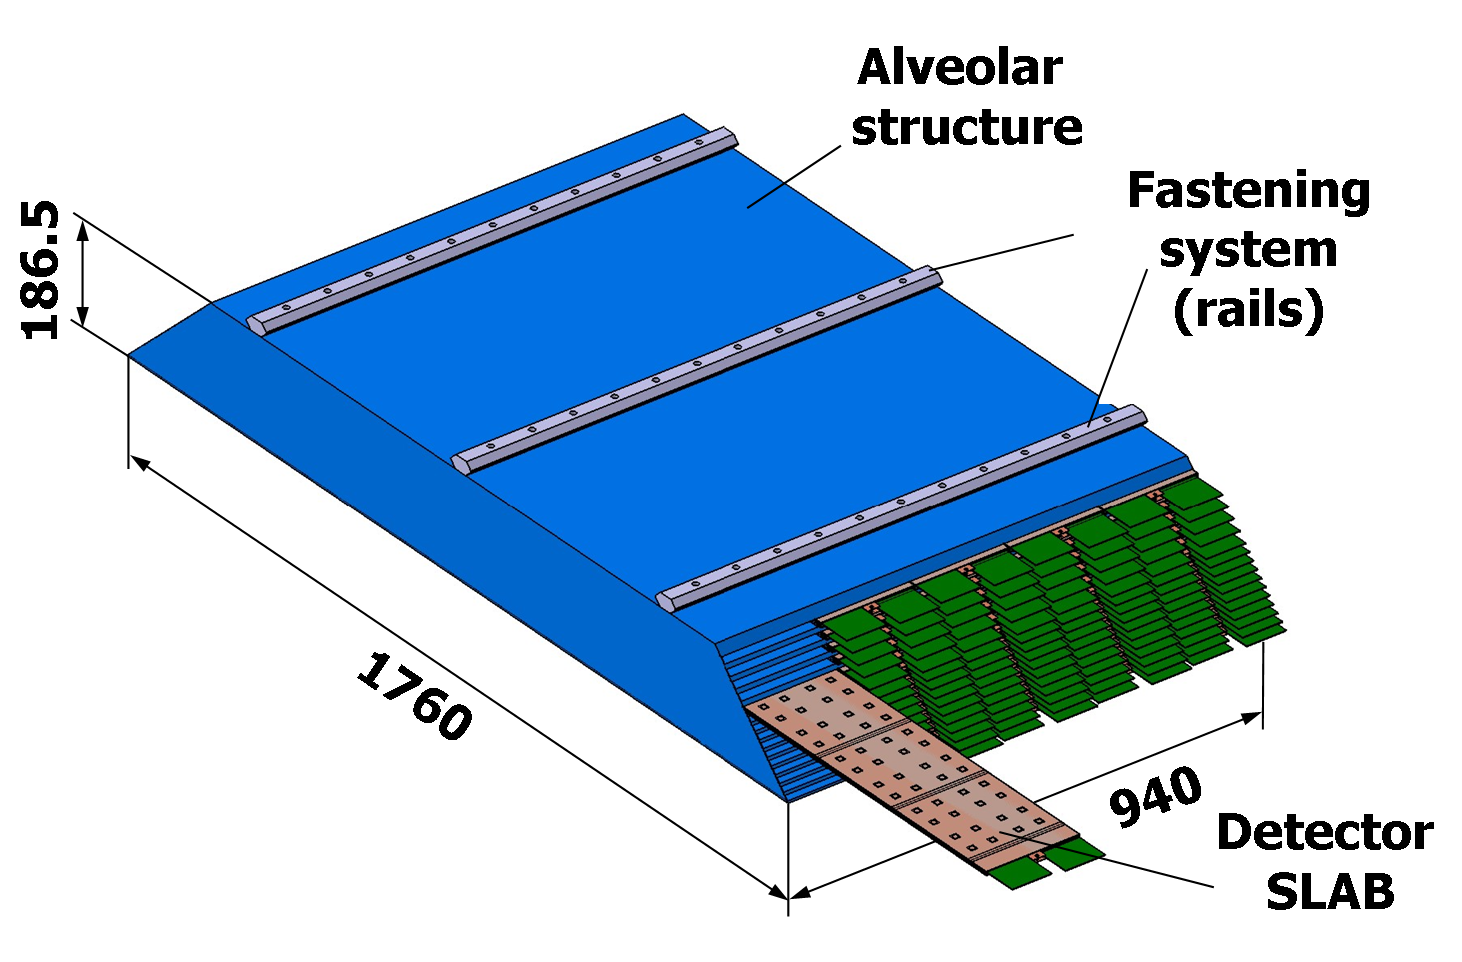
\includegraphics[height=5.5cm]{Experiments/fig/ECALview_module_annot} 
  \end{tabular}
  \caption[ECAL Structure]{The Overall ILD Structure (left) and one individual module (right).The ECAL is made up 40 modules, each containing 30 detector slabs. The modules are combined into groups of 5 referred to as a stave which extend along the full length of the barrel. There are then 8 of these staves arranged in a circle to create the circumference of the barrel \cite{ILD}.}
  \label{Fig:ECAL}
\end{figure}

Later on (see \refsec{sect:DECAL}) we will discuss our work on developing an alternative form of the silicon pixel technology with ultra high granularity 50x50~$\mu^2$m pixels which acts as a digital machine and purely counts the number of particles absorbed in the active medium from the showering in the absorber and deduces the energy of the original particle from this.  This form of the technology has already begun to be studied \cite{2011JInst...6.5009B}. It is expected to be cheaper than the standard silicon pixel tehnology as it is based on \ac{CMOS} technology which is already mass produced commercially, and has the potential for improved performance over it's analogue counterpart due to reduced sensitivity to landau fluctuations.

\subsubsection{HCAL}

\begin{figure}[h]
  \centering
  \begin{tabular}[c]{cc}
    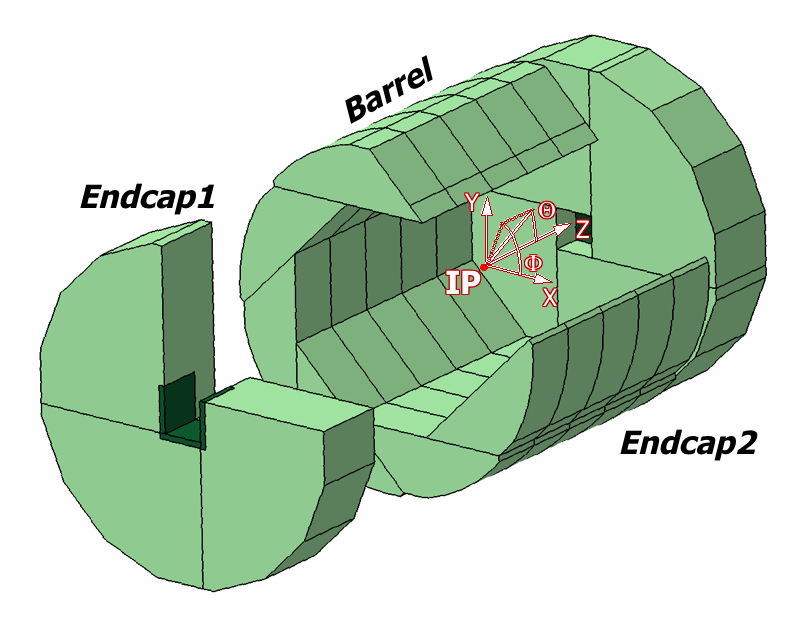
\includegraphics[height=5.5cm]{Experiments/fig/DHCALview_global.png} &
    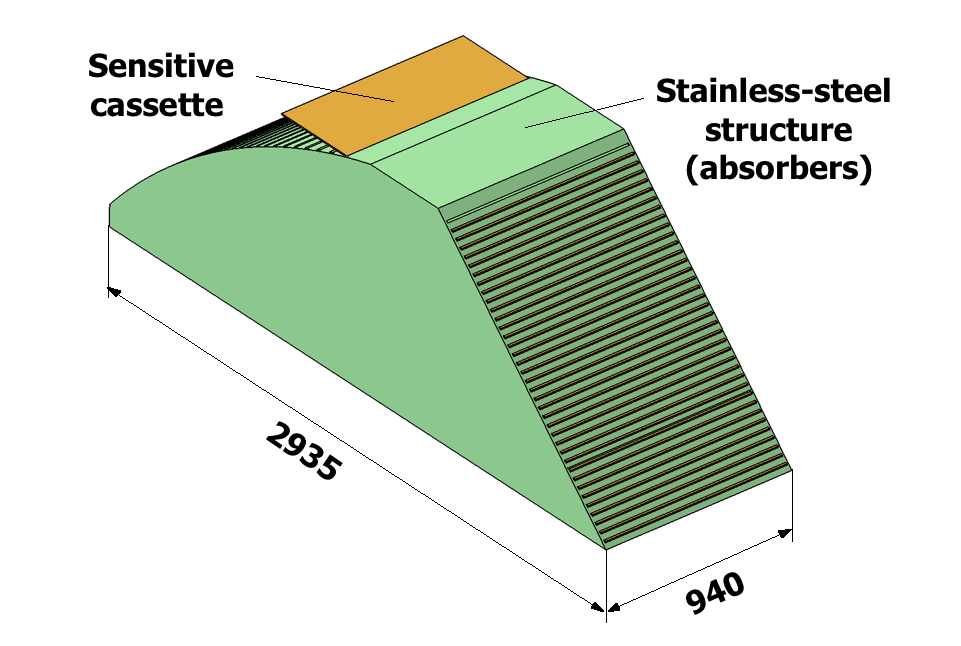
\includegraphics[height=5.5cm]{Experiments/fig/DHCALview_module.png}
  \end{tabular}
  \caption[HCAL Structure]{The Overall ILD HCAL Structure (left) and one individual module (right).The HCAL is made up 40 modules, each containing 30 detector slabs. The modules are combined into groups of 5 referred to as a stave which extend along the full length of the barrel. There are then 8 of these staves arranged in a circle to create the circumference of the barrel \cite{ILD}.}
  \label{fig:HCAL}
\end{figure}

The \ac{HCAL} is immediately outside the ECAL at r=2058 mm and has a similar overall modular structure to the \ac{ECAL} as shown in \reffig{fig:HCAL}. Each module consists of 48 stainless steel absorber plates of thickness 20 mm interspaced with 3 mm silicon scintillators with a transverse segmentation of 30x30 mm$^2$. This gives the \ac{HCAL} a total depth of $\sim$5 $\lambda_I$ (where $\lambda_I$ is the nuclear interaction length, the equivalent of $\chi_0$ for hadronic showers, which is typically much longer than $\chi_0$) and an energy resolution of 49\%/$\sqrt{E}$.

\subsubsection{Muon Detection}
Muon detection is perhaps the easiest process to perform at the ILC. Because the event environment at the ILC is typically clean with few high energy particles, few particles other than muons are capable of penetrating through the inner detector layers and the coil generating the magnetic field. As a result the muon detetors are produced by instrumenting the return yolk (r=4424 mm) that already surrounds the detector to contain the magnetic field. The number of muons produced in an event is also relatively small which means that the cell size for the muon detectors can be moderately large without the risk of multiple occupancy. The instrumentation is done by placing 10 layers of resistive plate chambers into the return yolk with strip sizes of the order 3-4 cm. This system is sufficient for accurately detecting muons and contributing to the measurement of their momentum. This system provides $\sim$100\% efficiency for identifying muons with momentum $>$3 GeV. Below this the muons do not have enough penetrating power to traverse through the yolk. This identification performance can extended down to 1.5 GeV when information from the calorimeters is included as well.

\subsection{CLIC ILD}

At \ac{CLIC} the detector designs were orginally based on the two \ac{ILC} detectors, \ac{ILD} and \ac{SiD}, but with a few changes to adapt for the different experimental conditions at \ac{CLIC}. In the case of \ac{ILD}, due to the large beam related backgrounds the vertex detectors were moved to be 15 mm further from the \ac{IP} to avoid pixel saturation. To account for the higher energy jets produced in interactions, the \ac{HCAL} depth was extended to 7.5 $\lambda_I$ to reduce leakage out of the back of the detector. To avoid increasing the radius of the magnetic solenoid (one of the main driving costs of the whole detector) the choice of absorber material in the \ac{HCAL} was switched to tungsten to provide the increased interaction length but over the same depth as in the orignal steel design. In the barrels, because the thickness does not affect the solenoid radius, the absorber was left as steel. To improve the charge identification of higher energy tracks, the magnetic field strength was changed to be 4T which was found to still be achievable using the original \ac{ILD} solenoid design. Further details on the CLIC version of \ac{ILD} can be found in the \ac{CLIC} \ac{CDR}\cite{CDR}.

This version of the \ac{ILD} detector is used for the analyses presented in Chapters \ref{Higgs Analysis} and \ref{chapter:topanalysis}. Since these analyses have been conducted, \ac{CLIC} has recently produced a new unified detector design that will be used for future studies. Overall the design is similar to that of \ac{ILD} but with a deeper \ac{ECAL} to allow for higher energy photon containment and the tracker has been changed from a \ac{TPC} to an all silicon tracker. As this version is not used in the studies presented here we will not give a detailed account of the detector but more information is avilable in \cite{Pitters:2018jxt}. Overall the impact of the change in dedector design is expected to be negligible for the studies presented here.










\chapter{Theory}
\label{theory}

This thesis presents two new analyses of the prospects for measuring the $H\rightarrow WW$ branching ratio and the forward-backward asymmetry in \ttbar production at CLIC during the 1.4~TeV operational stage. It is therefore important to understand the physics behind these measurements and examine their significance in the context of the physics programme of both CLIC and the wider state of particle physics.


\section{The Standard Model}

The \ac{SM} is a quantum field theory representing our current description of fundamental particles and the interactions between them. It consists of twelve spin-$\frac{1}{2}$ fermions (and their corresponding antiparticles), five spin 1 gauge bosons and one spin 0 scalar boson (as shown in \reffig{tab:smparticles}) where the interactions of the model are described by an $SU(3)_{C}\oplus SU(2)_{L}\oplus SU(1)_{Y}$ local gauge symmetry. The model describes point like particles which interact via the strong, weak and electromagnetic forces. No gravitational interactions are described within the model.

\begin{table}
  \centering
  \begin{tabular}{l c c c c}
    \toprule
    Type  & Name & Mass & Charge (e) & Spin  \\
    \midrule
    Quark & Up & 2.2$^{+ 0.6}_{-0.4}$ MeV & +2/3 & 1/2 \\
    Quark & Down & 4.7$^{+ 0.5}_{-0.4}$ MeV &  -1/3 & 1/2 \\
    \midrule
    Quark & Charm & 1.28$^{+ 0.3}_{-0.3}$ GeV& +2/3 & 1/2 \\
    Quark & Strange & 96$^{+ 8}_{-4}$ MeV& -1/3 & 1/2 \\
    \midrule
    Quark & Top & 173.4$^{+ 1.1}_{-1.1}$ GeV & +2/3 & 1/2 \\
    Quark & Bottom & 4.18$^{+ 0.04}_{-0.03}$ GeV& +1/3 & 1/2 \\
    \midrule
    \midrule
    Lepton & Electron & 0.5109989461$\pm$0.0000000031 MeV & -1 & 1/2 \\
    Lepton & Muon & 105.6583745$\pm$0.0000024 MeV& -1 & 1/2 \\
    Lepton & Tau & 1776.86$\pm$0.12 MeV & -1 & 1/2 \\
    \midrule
    Lepton & Electron Neutrino & $<$2 eV & 0 & 1/2 \\
    Lepton & Muon Neutrino & $<$2 eV & 0 & 1/2 \\
    Lepton & Tau Neutrino & $<$2 eV & 0 & 1/2 \\
    \midrule
    \midrule
    Gauge Boson & W$^+$ & 80.385$\pm$0.015 GeV& 1 & 1 \\
    Gauge Boson & Z & 91.1876$\pm$0.0021 GeV & 0 & 1 \\
    Gauge Boson & $\gamma$ & 0 & 0 & 1 \\
    Gauge Boson & gluon & 0 & 0 & 1 \\
    \midrule
    \midrule
    Scalar Boson & Higgs & 125.09$\pm$0.24 GeV & 0 & 0 \\
    \bottomrule
  \end{tabular}
  \caption[Particles of the Standard Model]{Particles of the Standard Model \cite{Patrignani:2016xqp}}
  \label{tab:smparticles}
\end{table}

The fermions of the model can be classified into two families, leptons and quarks, according to how they interact. The quark family consists of the up(u), down(d), charm(c), strange(s), top(t) and bottom(b) quarks, all of which are capable of interacting via the strong, weak and electromagnetic forces. The lepton family, consisting of the electron(e), muon($\mu$), tau($\tau$), electron neutrino($\nu_{e}$), muon neutrino($\nu_{\mu}$) and tau neutrino($\nu_{tau}$), are defined by the fact they carry no color charge and so are incapable of interacting via the strong force, however they all interact via the weak force and the $e$/$\mu$/$\tau$ can interact electromagnetically. The gauge bosons are the mediators of the three fundamental forces of the model. The photon is a massless boson that mediates the electromagnetic force by coupling to particles with electrical charge. The gluon is also massless and mediates the strong force by coupling to particles with color charge. The gluon is unique amongst the gauge bosons in that it is the only boson that carries the charge to which it couples (i.e. it is colored) and so couples to itself. One direct consequence of this is that it is impossible to form a stable colored state due to color confinement and so quarks are only observed in net-colorless states called hadrons. When a quark is produced in an interaction, it will typically undergo a process known as hadronization in which the quark will bind to quarks/antiquarks spontaneously produced from the vacuum to form quark-antiquark pairs known as mesons, or triplets of quarks or antiquarks known as baryons. The only exception to this is the top quark which will typically decay on a far shorter timescale than is needed for hadronization to occur. The final three gauge bosons are the Z, W$^+$ and W$^-$ which are all massive and mediate the weak interaction via their coupling to weak isospin.

Much like the fermions can be separated into quarks and leptons according to the way they interact, the underlying symmetry of the \ac{SM} of $SU(3)_{C}\oplus SU(2)_{L}\oplus SU(1)_{Y}$ can be decomposed into separate parts according to the interactions that the symmetries describe. The $SU(3)_{C}$ group represents transformations of the color state of a system and so describes interactions involving the strong force. These interactions are commonly referred to as \ac{QCD}. The $SU(2)_{L}\oplus SU(1)_{Y}$ symmetry represents electroweak theory- a unified description of the weak and electromagnetic interactions. In this description, fermions can be thought of as consisting of left and right handed fields, where the left handed components transform as doublets under SU(2) transformations while the right handed components only transform as singlets. The result of this is that the weak interaction only acts on the left handed field components. Hence the weak force only couples to left(right) handed particles (antiparticles.) 

One of the most interesting features of electroweak theory occurs when considering the effect of gauge transformations on the Lagrangian of the system. In quantum field theory, fermions can be described by a Dirac field with the following Lagrangian\cite{Pich:2005mk}

\begin{equation}
  \label{eq:diracLagrangian}
\mathscr{L}=i\bar{\psi}(x) \gamma^{\mu} \partial{_\mu} \psi(x)  -m\bar{\psi}(x)\psi(x),
\end{equation}

Applying a global phase transition of the form

\begin{equation}
\psi(x) \rightarrow \psi '(x) = e^{iQ\alpha}\psi(x),
\end{equation}

will leave the Lagrangian unchanged due to the fact $e^{i\alpha}\psi e^{-i\alpha}\psi=1$. However, in the case of local gauge transformations we replace the global phase transformation by a local one i.e. $\alpha \rightarrow\alpha(x) $ i.e. the phase has a local space-time dependence, then \refeq{eq:diracLagrangian} is no longer invariant as

\begin{equation}
  \partial{_\mu} \psi(x)\rightarrow e^{iQ\alpha(x)} (\partial{_\mu} + iQ\partial{_\mu}\alpha(x)) \psi(x).
\end{equation}

In order to restore the invariance, the derivative $\partial{\mu}$ must be replaced with the covariant derivative $D_{\mu}$ which is of the form

\begin{equation}
  D_{\mu}=\partial{_\mu}+ieA_{\mu},
\end{equation}

where $A_{\mu}$ is a gauge field which transforms as

\begin{equation}
  A_{\mu}\rightarrow A_{\mu}^{'} = A_{\mu} - \frac{1}{e}\partial{_\mu}\alpha(\textbf{x}).
\end{equation}

In electroweak theory the gauge fields required are found to consist of three weak isospin fields, $W_1, W_2$ and $W_3$,  coming from the SU(2) group and one weak hypercharge field, B, from U(1). The interesting result of this is the prediction that the bosons associated with these fields and the fermions they interact with should be massless. However, this is not supported by data as the bosons of the weak force, Z and W, have masses of $m_Z$=91.876 $\pm$ 0.0021 GeV and $m_W$=80.385 $\pm$ 0.015 GeV respectively\cite{Patrignani:2016xqp}. Furthermore, in electroweak theory it can be shown that the presence of massive electroweak bosons results in unphysical predictions in the \ac{SM} e.g. violation of unitarity when calculating the amplitude of $WW\rightarrow WW$ scattering \cite{Szleper:2014xxa}. These problems can be fixed via consideration of the final particle within the \ac{SM}, the Higgs boson.

\section{The Higgs Boson and the Origin of Mass}

To solve the problems seen in the electroweak sector, Brout, Englert and Higgs \cite{PhysRevLett.13.508}\cite{PhysRevLett.13.321} proposed that mass terms could be generated within the \ac{SM} via the addition of a complex, scalar doublet of the group $SU(2)$ possessing four degrees of freedom

\begin{equation}
\phi = \begin{pmatrix} \phi^{+} \\ \phi^{0} \end{pmatrix}, 
\end{equation}

with potential

\begin{equation}
V(\phi) = \mu^{2}\phi^{\dagger}\phi + \frac{\lambda^{2}}{2}(\phi^{\dagger}\phi)^{2},
\end{equation}

where $\mu^{2}$ is the negative mass squared parameter and $\lambda$ is the Higgs field self-coupling.

The Higgs field is found to interact with the $W_{1},W_{2},W_{3}$ and $B$ gauge fields. In the case that $\mu^{2}<0$, due to the Higgs field acquiring a non-zero expectation value, the $SU(2)_{L}\oplus SU(1)_{Y}$ symmetry is found to break leaving only a $U(1)_{em}$ symmetry corresponding to a massless photon. Of the four degrees of freedom associated with the Higgs field, the interaction of the field with the W and B gauge fields results in three massive gauge bosons corresponding to the measured $Z$ and $W^{\pm}$ masses, where the physically observed bosons actually represent mixtures of the underlying gauge fields

\begin{equation}
\gamma = \cos\theta_{W}B  +\sin\theta_{W}W_{3}, 
\end{equation}

\begin{equation}
Z = \cos\theta_{W}W_{3}  -\sin\theta_{W}B,
\end{equation}

\begin{equation}
W^{\pm}= \frac{1}{\sqrt{2}}(W_{1}\mp iW_{2}),
\end{equation}

and where $\theta_{W}$ is the weak mixing angle.

The last remaining degree of freedom of the Higgs field corresponds to the Higgs boson itself. The mass of the Higgs boson can be determined to be $m_{H}=\sqrt{2\lambda}\nu$, where $\nu$ is the vacuum expectation value for the Higgs field. While $\nu$ can be calculated within the standard model, $\lambda$ is a free parameter and so the mass of the Higgs is not known a priori. Experimentally it is found to be $\sim$125GeV\cite{:2012gk,Chatrchyan:2012xdj}.

While the mass of the Higgs is of special interest because its value is a free parameter in the standard model, there are many more properties of the Higgs that are important to measure. In particular, the way in which the Higgs boson couples to other particles is predicted without ambiguity within the \ac{SM} and is expected to vary between various \ac{BSM} models. Within the \ac{SM} the coupling of the Higgs to fermions and bosons varies according to their masses


\begin{equation}
g_{Hf\bar{f}}=\frac{M_f}{\nu} ~~~~~~~~    g_{HBB}=\frac{2M_B^2}{\nu} .
\end{equation}

Therefore, characterizing the coupling to each fermion as a function of the fermions mass represents a powerful way of testing the \ac{SM}. The mass dependence on the Higgs couplings also presents a new way to perform indirect searches for new physics involving as yet unseen massive particles by looking at the branching ratio of Higgs decays to invisible decay products and the total Higgs decay width. This is of particular interest in searches for dark matter which is known to interact gravitationally and so must possess mass. 

\section{Higgs Measurements at CLIC}
\begin{figure}
  \centering
  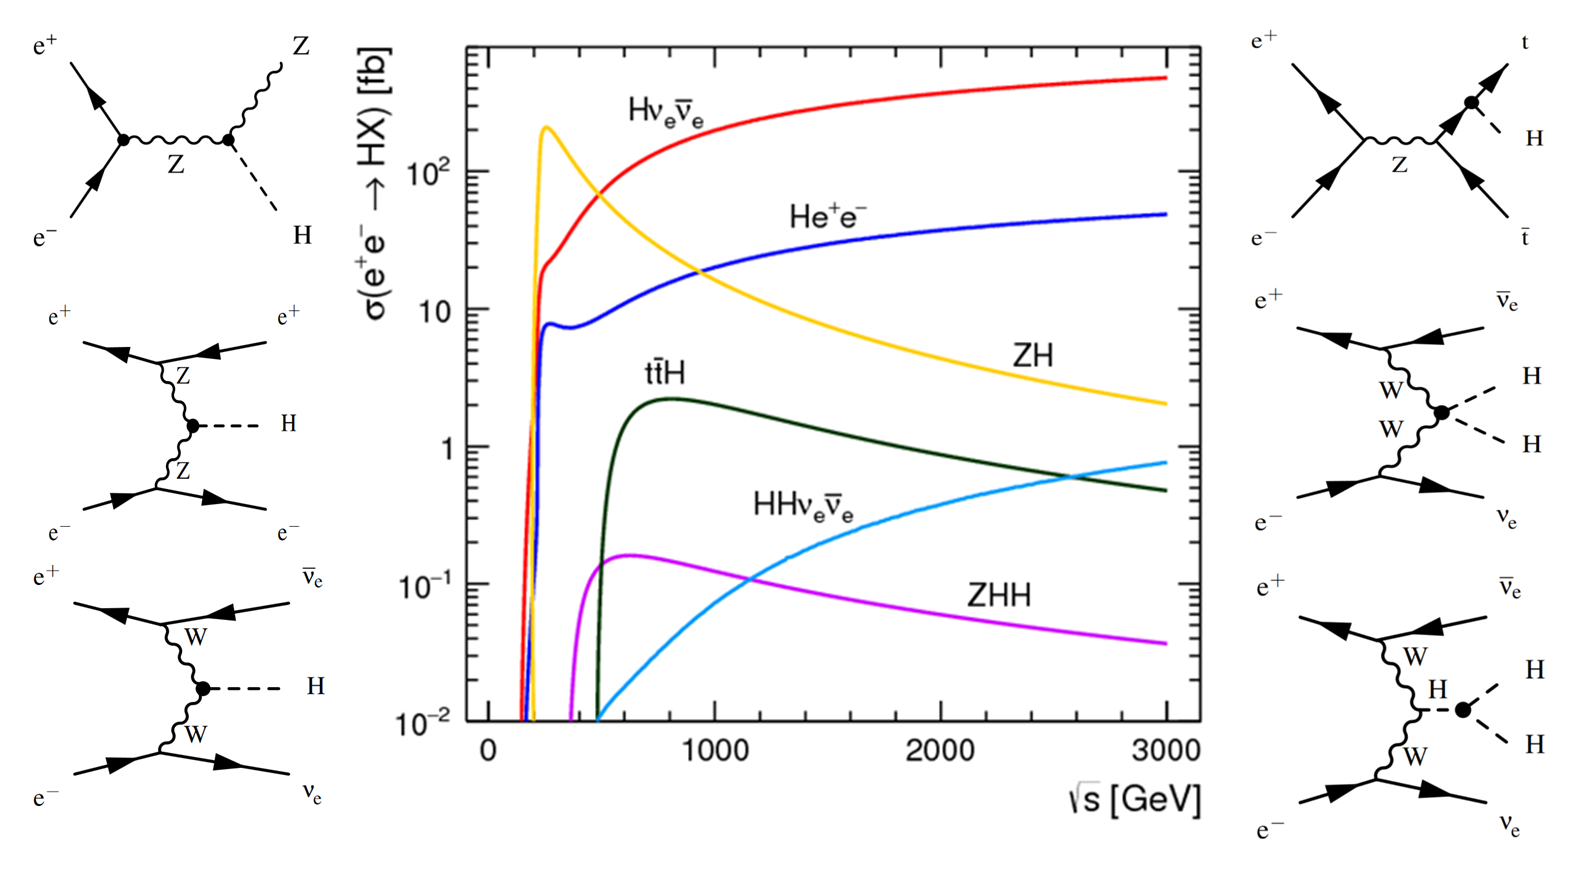
\includegraphics[width=0.95\textwidth,keepaspectratio]{Theory/fig/HiggsProcessesExtra.png}
  \caption[Cross sections for Higgs production mechanisms]{Cross sections for Higgs production mechanisms \cite{Abramowicz:2016zbo}.}
  \label{fig:higgsXSecs}
\end{figure}

The CLIC physics programme places substantial emphasis on characterizing the Higgs boson as it presents a new and relatively less well measured sector of the \ac{SM} to explore. In particular it will aim to measure the mass, width, and couplings of the Higgs in a model independent manner. Electron positron collisions provide access to numerous Higgs production mechanisms which can be seen in \reffig{fig:higgsXSecs}. Due to the strong energy dependence on many of the cross sections on energy, different processes will be of interest at each of the three energy stages operated at CLIC. At 380GeV the focus will predominantly be on measuring the Higgsstrahlung ($ZH$) process in which a Z boson radiates a Higgs, while at higher energies vector boson fusion ($H\nu\bar{\nu},He^{+}e^{-}$) dominates and new processes such as di-Higgs production become accessible. A summary of all the results from current Higgs studies performed by CLIC is available in \cite{Abramowicz:2016zbo}.

\subsection{Higgsstrahlung}

\begin{figure}
  \centering
  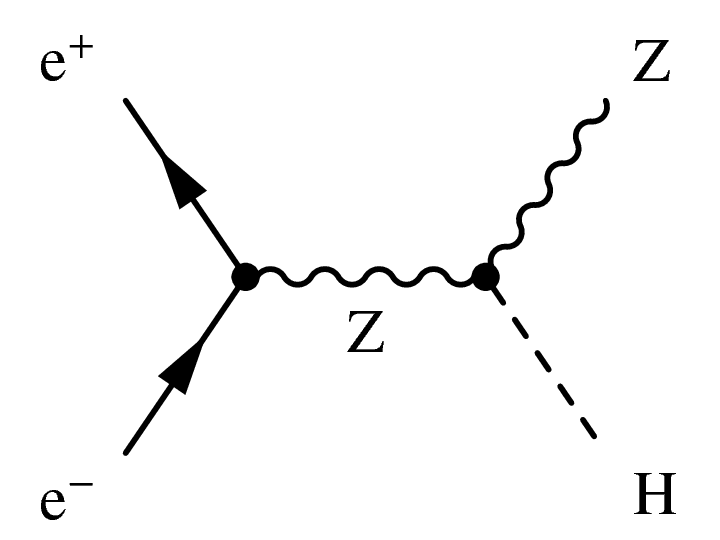
\includegraphics[width=0.45\textwidth,keepaspectratio]{Theory/fig/HiggsStrahlung.png}
  \caption[The Higgstrahlung Process]{The Higgstrahlung Process.}
  \label{fig:higgsstrahlung}
\end{figure}


One of the key aims of the experiment will be to examine the Higgsstrahlung process shown in \reffig{fig:higgsstrahlung}. In this process, if the four-momentum of the Z boson can be measured to high precision, then because the initial conditions of the collision are well known, one can determine the mass of the particle it is recoiling against ($m_{rec}^{2} = s + m_{z}^{2} - 2E_{z}\sqrt{s}$, with $E_Z$ being the measured energy of the Z) and infer the presence of a Higgs boson on an event-by-event basis. This allows properties such as the Higgs mass, cross-section and coupling to the Z to be measured without actually using the decay products of the Higgs boson directly, which in turn allows the measurements to be model independent. This method is not possible at hadron colliders such as the LHC where, even though the Higgsstrahlung process still occurs, the four momentum of the colliding particles can never be known as precisely due to their composite nature. Using the clean signal from cases where the Z decays to a pair of muons or electrons it is possible to measure the recoil mass to high precision and thus determine the mass of the Higgs to $\Delta m_{H} = 110$~MeV (see \reffig{fig:higgsmass}) using data from the low energy stage only. This value can be further improved to $\Delta m_{H} = 44~MeV$ when including direct measurement results from the $ee\rightarrow H\nu\bar{\nu}, H\rightarrow b\bar{b}$ channel at 3~TeV. Despite giving a poorer resolution on the Z four momentum, the $Z\rightarrow qq$ higgsstrahlung channel is also considered due to its larger cross section. Using this channel a limit of $BR(H\rightarrow invis.) <0.97\%$ at 90\% C.L. can be set. 

\begin{figure}
  \centering
  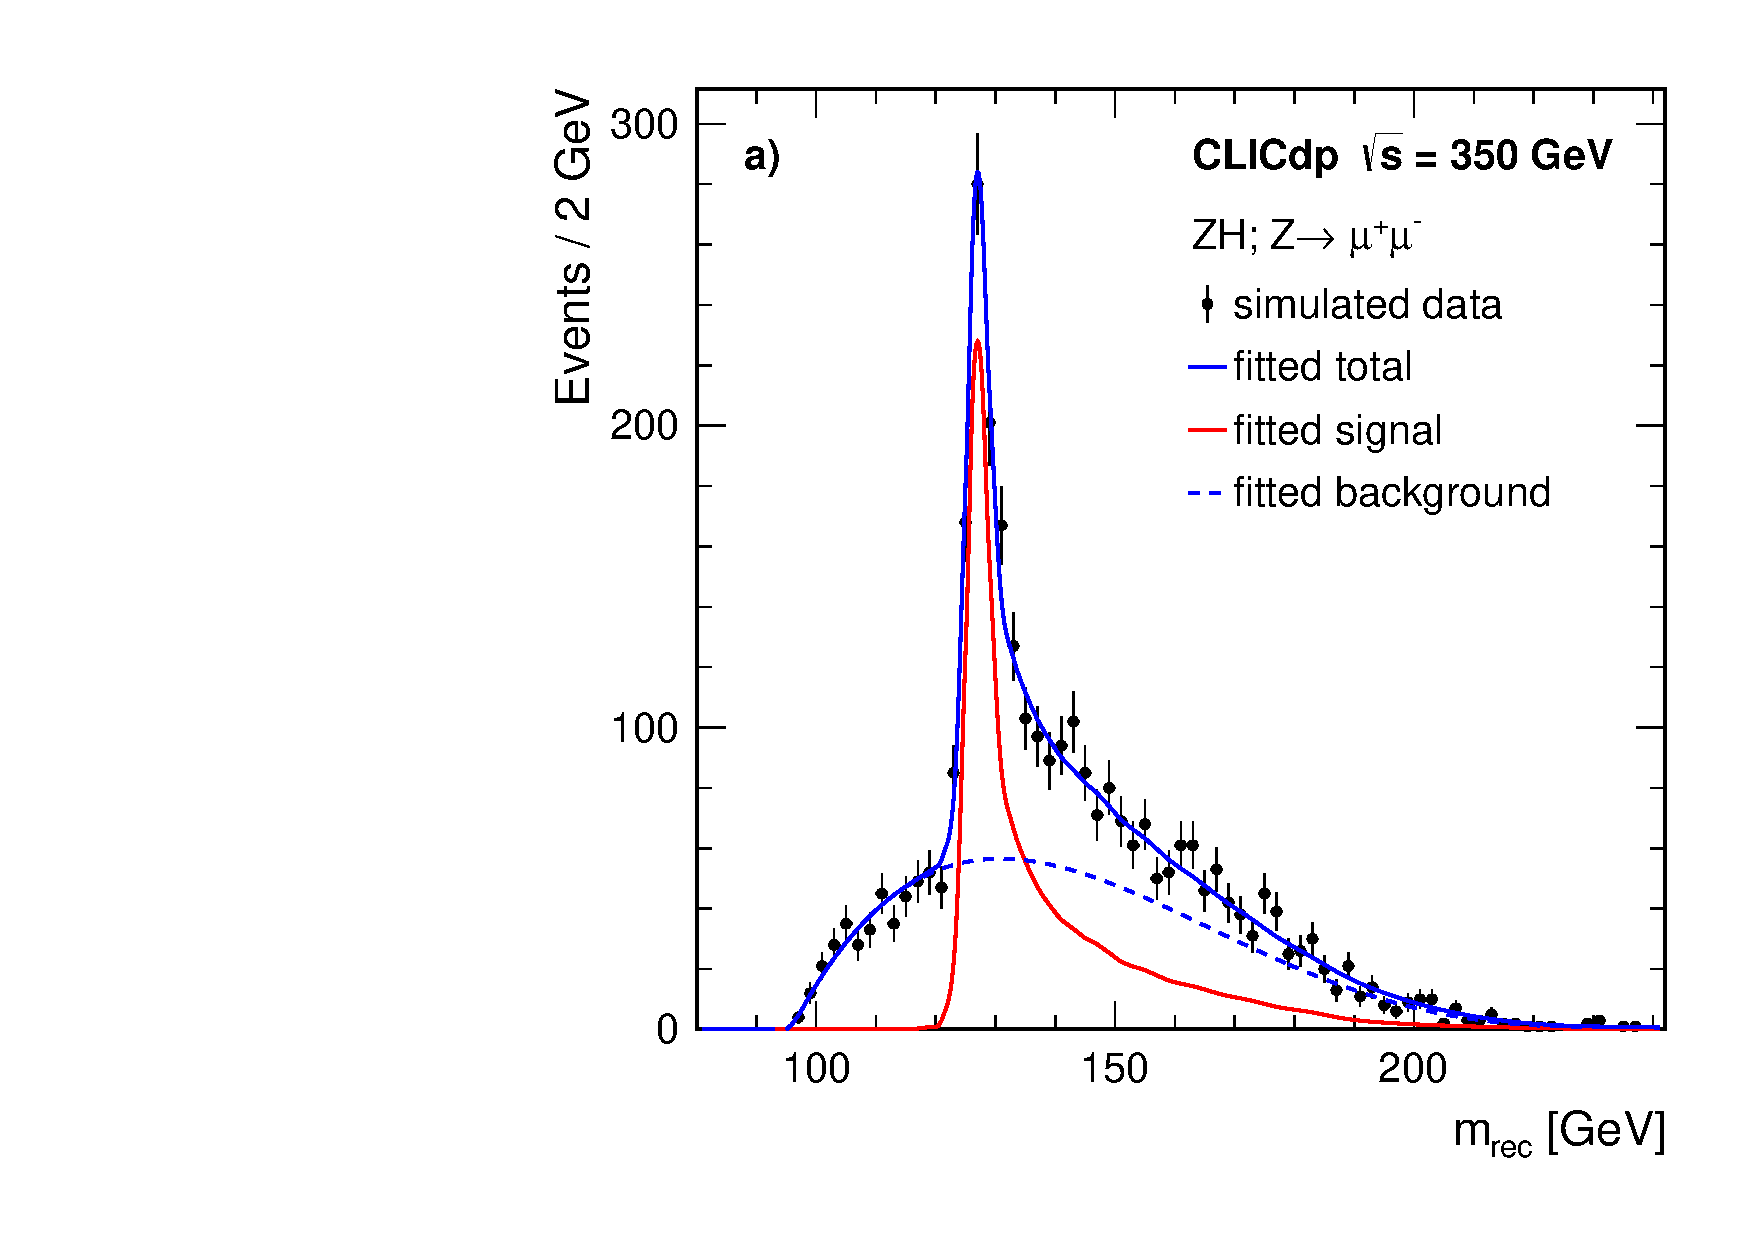
\includegraphics[width=0.45\textwidth,keepaspectratio]{Theory/fig/350GeV_Recoil_mumuX_MrecoilFit.pdf}
  \caption[Reconstructed recoil mass from Higgsstralung process]{Reconstructed recoil mass from Higgsstralung process \cite{Abramowicz:2016zbo}.}
  \label{fig:higgsmass}
\end{figure}

 
\subsection{Model Independent Extraction of Higgs Couplings}


While the Higgsstrahlung alone allows the mass and branching ratios of the Higgs to be determined, it is further possible to extract the absolute width of the Higgs, $\Gamma_H$, by measuring the rates of several different Higgs processes and combining them in the right ratio. One such scheme proposed for doing this is shown in \refeq{modelindependentformula} \cite{Durig:2014lfa}

\begin{equation}
  \label{modelindependentformula}
  \Gamma_H = \frac{X_1^2X_3^2}{X_4^2X_2},
\end{equation}

where

\begin{equation}
X_1=\sigma_{ZH} \propto g_{HZZ}^2
\end{equation}

\begin{equation}
  \label{X2}
  X_2=\sigma_{H\nu\bar{\nu}} \times BR(H\rightarrow WW^*) \propto \frac{g_{HWW}^4}{\Gamma_H}
\end{equation}

\begin{equation}
X_3=\sigma_{H\nu\bar{\nu}} \times BR(H\rightarrow b\bar{b}) \propto \frac{g_{HWW}^{2}g_{Hbb}^2}{\Gamma_H}
\end{equation}

\begin{equation}
X_4=\sigma_{ZH} \times BR(H\rightarrow b\bar{b}) \propto \frac{g_{HZZ}^{2}g_{Hbb}^2}{\Gamma_H}
\end{equation}

 With the exception of $X_1$, the choice of variables used is not unique (e.g. one could replace the production mechanism in $X_1$ and $X_2$ with ZZ-fusion rather than WW-fusion,) however the combination shown here is expected to give the highest precision on $\Gamma_H$ due to the large cross-section associated with WW-fusion and the high branching ratio of $H\rightarrow b\bar{b}$ ($\sim$ 65\%). In chapter \ref{Higgs Analysis} we will present our research on the precision with which $X_2$ can be measured during the 1.4~TeV run at CLIC. Currently at the LHC the standard process for extracting couplings from the equivalent measurements of $X_{2,3\&4}$ is to multiply through by the standard model value of the Higgs width \cite{ATLAS-CONF-2015-044}. This type of measurement is referred to as ``model-dependent'' as the values determined for the Higgs couplings implicitly assume the \ac{SM} Higgs width. At CLIC, because the width can be measured experimentally there is no need to make this assumption and so the couplings are measured in a ``model-independent'' way. The unique ability of $e^+e^-$ colliders to perform model-independent measurements is one of the largest driving factors for constructing and using them as a so called ``Higgs-Factory''. One limiting factor for the model-independent measurements of the couplings is that they are always ultimately dependent on the precision with which the ZH cross section can be measured (predicted to be $\Delta h_{HZZ} = 0.8\%$\cite{Abramowicz:2016zbo}) as this quantity is always needed in the ratio used to extract $\Gamma_H$.

\begin{table}
  \centering
  \begin{tabular}{lllc}\toprule
     &                                                           &                              & Statistical precision                        \\\cmidrule(l){4-4}
     Channel  & Measurement                                        & Observable            & $350\,\GeV$       \\ 
     &                                                           &                              & $500\,fb^{-1}$        \\ \midrule
     $ZH$            & Recoil mass distribution                                  & $\mH$                        & $110\,\MeV$  \\
     $ZH$            & $\sigma(ZH)\times BR(H\rightarrow \text{invisible})$         & $\Gamma_\text{inv}$          & $0.6\,\%$  \\ \midrule
     $ZH$            & $\sigma(ZH)\times BR(Z\rightarrow l^+l^-)$             & $g^{2}_{HZZ}$                  & $3.8\,\%$  \\
     $ZH$            & $\sigma(ZH)\times BR(Z\rightarrow q\bar{q})$                  & $g^{2}_{HZZ}$                  & $1.8\,\%$  \\
     $ZH$            & $\sigma(ZH)\times BR(H\rightarrow b\bar{b})$                & $g^{2}_{HZZ}g^{2}_{Hbb}/\Gamma_H$     & $0.86\,\%$ \\
     $ZH$            & $\sigma(ZH)\times BR(H\rightarrow c\bar{c})$                & $g^{2}_{HZZ}g^{2}_{Hcc}/\Gamma_H$       & $14\,\%$ \\
     $ZH$            & $\sigma(ZH)\times BR(H\rightarrow gg)$                   &                              & $6.1\,\%$ \\
     $ZH$            & $\sigma(ZH)\times BR(H\rightarrow \tau^+\tau^-)$               & $g^{2}_{HZZ}g^{2}_{H\tau\tau}/\Gamma_H$ & $6.2\,\%$ \\
     $ZH$            & $\sigma(ZH)\times BR(H\rightarrow WW^*)$                 & $g^{2}_{HZZ}g^{2}_{HWW}/\Gamma_H$     & $5.1\,\%$ \\
     $H\nu_e\bar{\nu_e}$    & $\sigma(H\nu_e\bar{\nu_e})\times BR(H\rightarrow b\bar{b})$        & $g^{2}_{HWW}g^{2}_{Hbb}/\Gamma_H$     & $1.9\,\%$ \\
     $H\nu_e\bar{\nu_e}$    & $\sigma(H\nu_e\bar{\nu_e})\times BR(H\rightarrow c\bar{c})$        & $g^{2}_{HWW}g^{2}_{Hcc}/\Gamma_H$     & $26\,\%$ \\
     $H\nu_e\bar{\nu_e}$    & $\sigma(H\nu_e\bar{\nu_e})\times BR(H\rightarrow gg)$        &     & $10\,\%$ \\    
     \bottomrule
   \end{tabular}
   \caption[Expected statistical uncertainties for Higgs measurements at 350~GeV at CLIC assuming unpolarised beams]{Expected statistical uncertainties for Higgs measurements at 350~GeV at CLIC assuming unpolarised beams \cite{Abramowicz:2016zbo}.}
   \label{fig:350GeVNumbers}
\end{table}

\begin{table}
  \centering
  \begin{tabular}{lllcc}\toprule
    &                                                           &                              & Statistical precision                       \\\cmidrule(l){4-5}
    Channel  & Measurement                                        & Observable & $1.4\,\TeV$         & $3\,\TeV$           \\ 
    &                                                           &                           & $1.5\,ab^{-1}$      & $2.0\,ab^{-1}$        \\ \midrule
    $H\nu_e\bar{\nu_e}$    & $H\rightarrow b\bar{b}$ mass distribution                       & $m_H$                & $47\,\MeV$     & $44\,\MeV$       \\ \midrule
    $H\nu_e\bar{\nu_e}$    & $\sigma(H\nu_e\bar{\nu_e})\times BR(H\rightarrow b\bar{b})$        & $g^{2}_{HWW}g_{Hbb}^{2}/\Gamma_H$   & $0.4\,\%$         & $0.3\,\%$           \\
    $H\nu_e\bar{\nu_e}$    & $\sigma(H\nu_e\bar{\nu_e})\times BR(H\rightarrow c\bar{c})$        & $g^{2}_{HWW}g_{Hcc}^{2}/\Gamma_H$  & $6.1\,\%$         & $6.9\,\%$           \\
    $H\nu_e\bar{\nu_e}$    & $\sigma(H\nu_e\bar{\nu_e})\times BR(H\rightarrow gg)$           &                     & $5.0\,\%$         & $4.3\,\%$           \\
    $H\nu_e\bar{\nu_e}$    & $\sigma(H\nu_e\bar{\nu_e})\times BR(H\rightarrow \tau^+\tau^-)$       & $g^{2}_{HWW}g_{H\tau\tau}^{2}/\Gamma_H$ & $4.2\,\%$         & $4.4\,\%$               \\
    $H\nu_e\bar{\nu_e}$    & $\sigma(H\nu_e\bar{\nu_e})\times BR(H\rightarrow \mu^+\mu^-)$       & $g^{2}_{HWW}g_{H\mu\mu}^{2}/\Gamma_H$   & $38\,\%$        & $25\,\%$            \\
    $H\nu_e\bar{\nu_e}$    & $\sigma(H\nu_e\bar{\nu_e})\times BR(H\rightarrow \gamma\gamma)$ &                          & $15\,\%$          & $10\,\%^*$               \\
    $H\nu_e\bar{\nu_e}$    & $\sigma(H\nu_e\bar{\nu_e})\times BR(H\rightarrow Z\gamma)$      &                             & $42\,\%$           & $30\,\%^*$               \\
    $H\nu_e\bar{\nu_e}$    & $\sigma(H\nu_e\bar{\nu_e})\times BR(H\rightarrow WW^*)$         & $g_{HWW}^{4}/\Gamma_H$            & $1.0\,\%$         & $0.7\,\%^*$         \\
    $H\nu_e\bar{\nu_e}$    & $\sigma(H\nu_e\bar{\nu_e})\times BR(H\rightarrow ZZ^*)$         & $g^{2}_{HWW}g_{HZZ}^{2}/\Gamma_H$  & $5.6\,\%$ & $3.9\,\%^*$   \\
    $He^+e^-$       & $\sigma(He^+e^-)\times BR(H\rightarrow b\bar{b)}$           & $g_{HZZ}^{2}g_{Hbb}^{2}/\Gamma_H$    & $1.8\,\%$ & $2.3\,\%^*$ \\ \midrule
    $t\bar{t}H$      & $\sigma(t\bar{t}H)\times BR(H\rightarrow b\bar{b})$          & $g_{Htt}^{2}g_{Hbb}^{2}/\Gamma_H$  & $8\,\%$         & $-$             \\
    $HH\nu_e\bar{\nu_e}$ & $\sigma(HH\nu_e\bar{\nu_e})$                               & $\lambda$                   & $54\,\%$          & $29\,\%$            \\
    $HH\nu_e\bar{\nu_e}$ & with $-80\,\%$ $e^-$ polarisation                             & $\lambda$                  & $40\,\%$          & $22\,\%$            \\ \bottomrule
  \end{tabular}
  \caption[Expected statistical uncertainties for Higgs measurements at 1.4~TeV and 3~TeV at CLIC assuming unpolarised beams]{Expected statistical uncertainties for Higgs measurements at 1.4~TeV and 3~TeV at CLIC assuming unpolarised beams \cite{Abramowicz:2016zbo}. Values marked with a * represent extrapolations from studies performed at 1.4~TeV.}
  \label{fig:HighENumbers}
\end{table}

\begin{figure}
  \centering
  \begin{subfigure}{.49\textwidth}
    \centering
    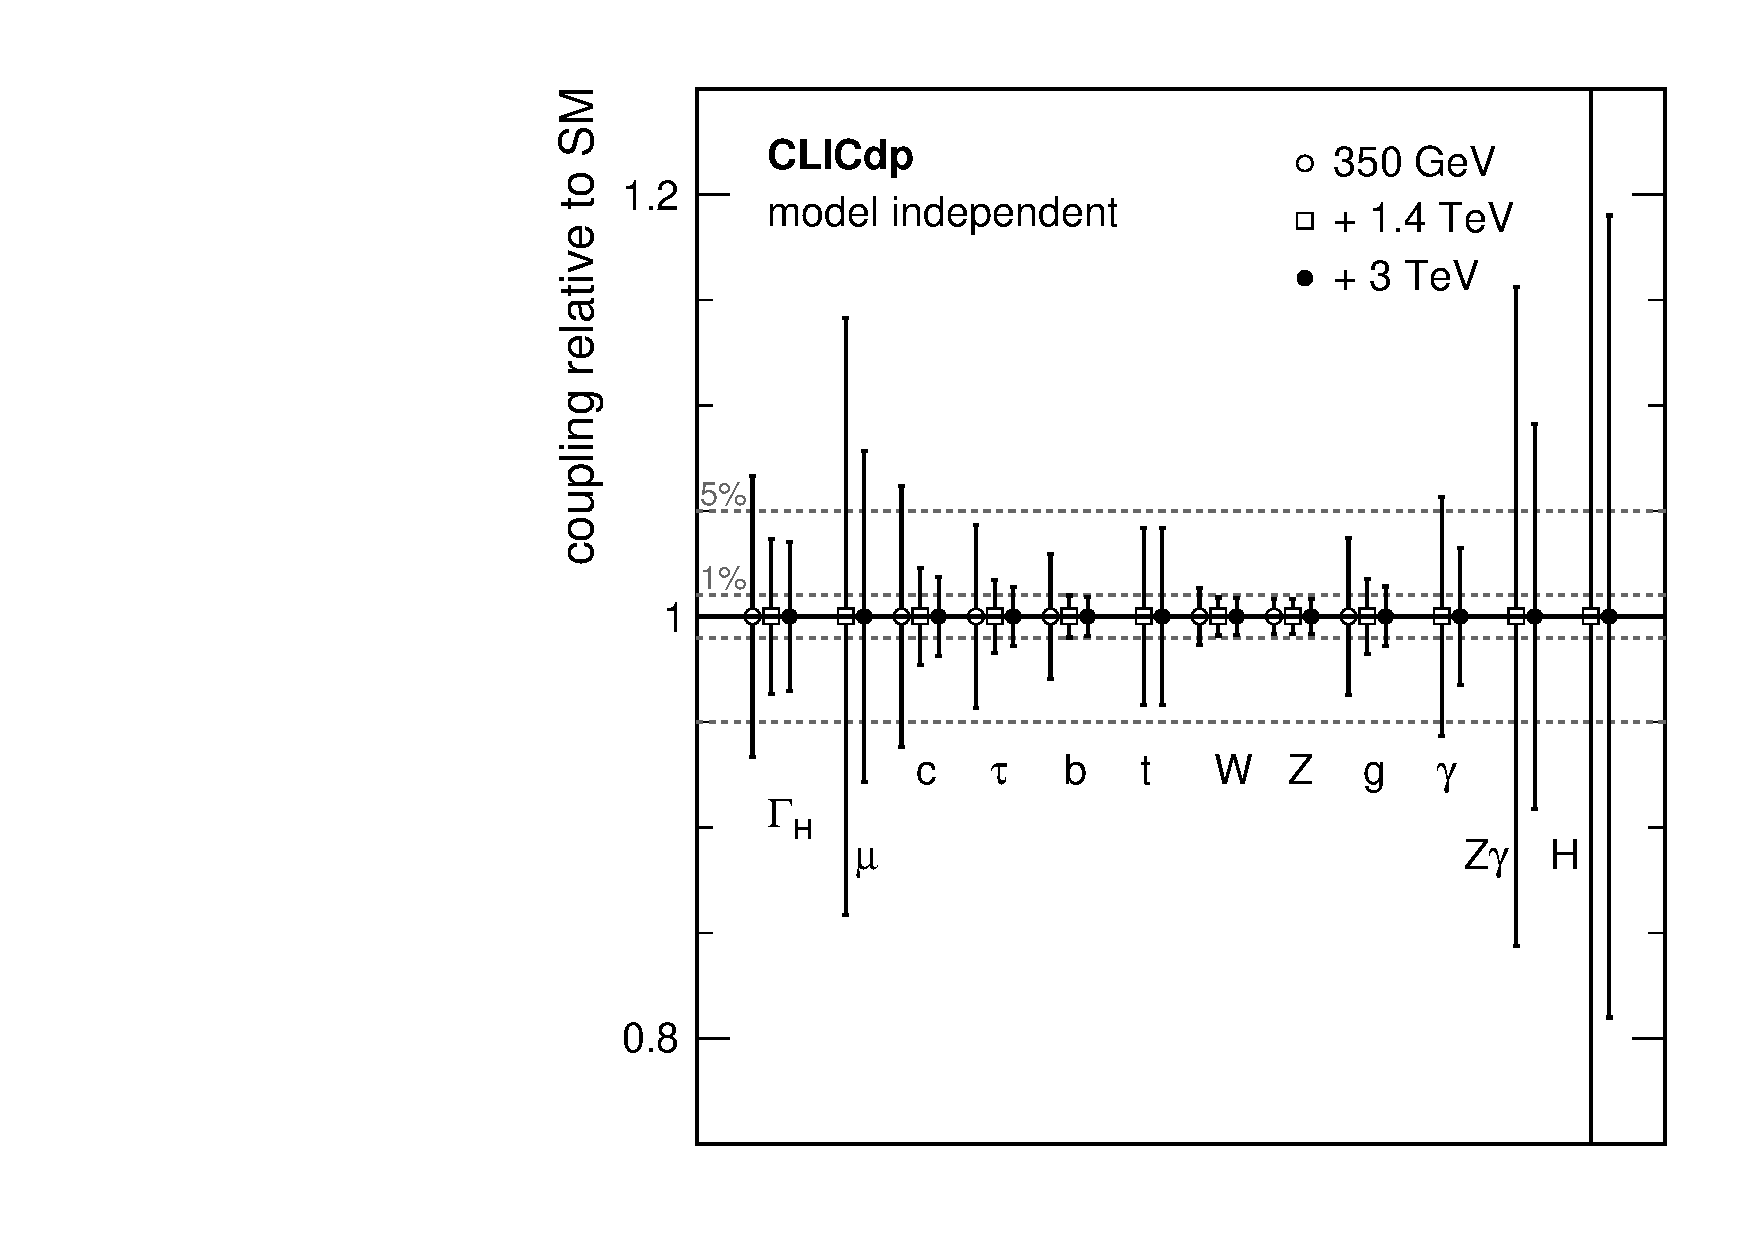
\includegraphics[width=0.95\linewidth]{Theory/fig/FitResultsMI.pdf}
  \end{subfigure}
    \begin{subfigure}{.49\textwidth}
    \centering
    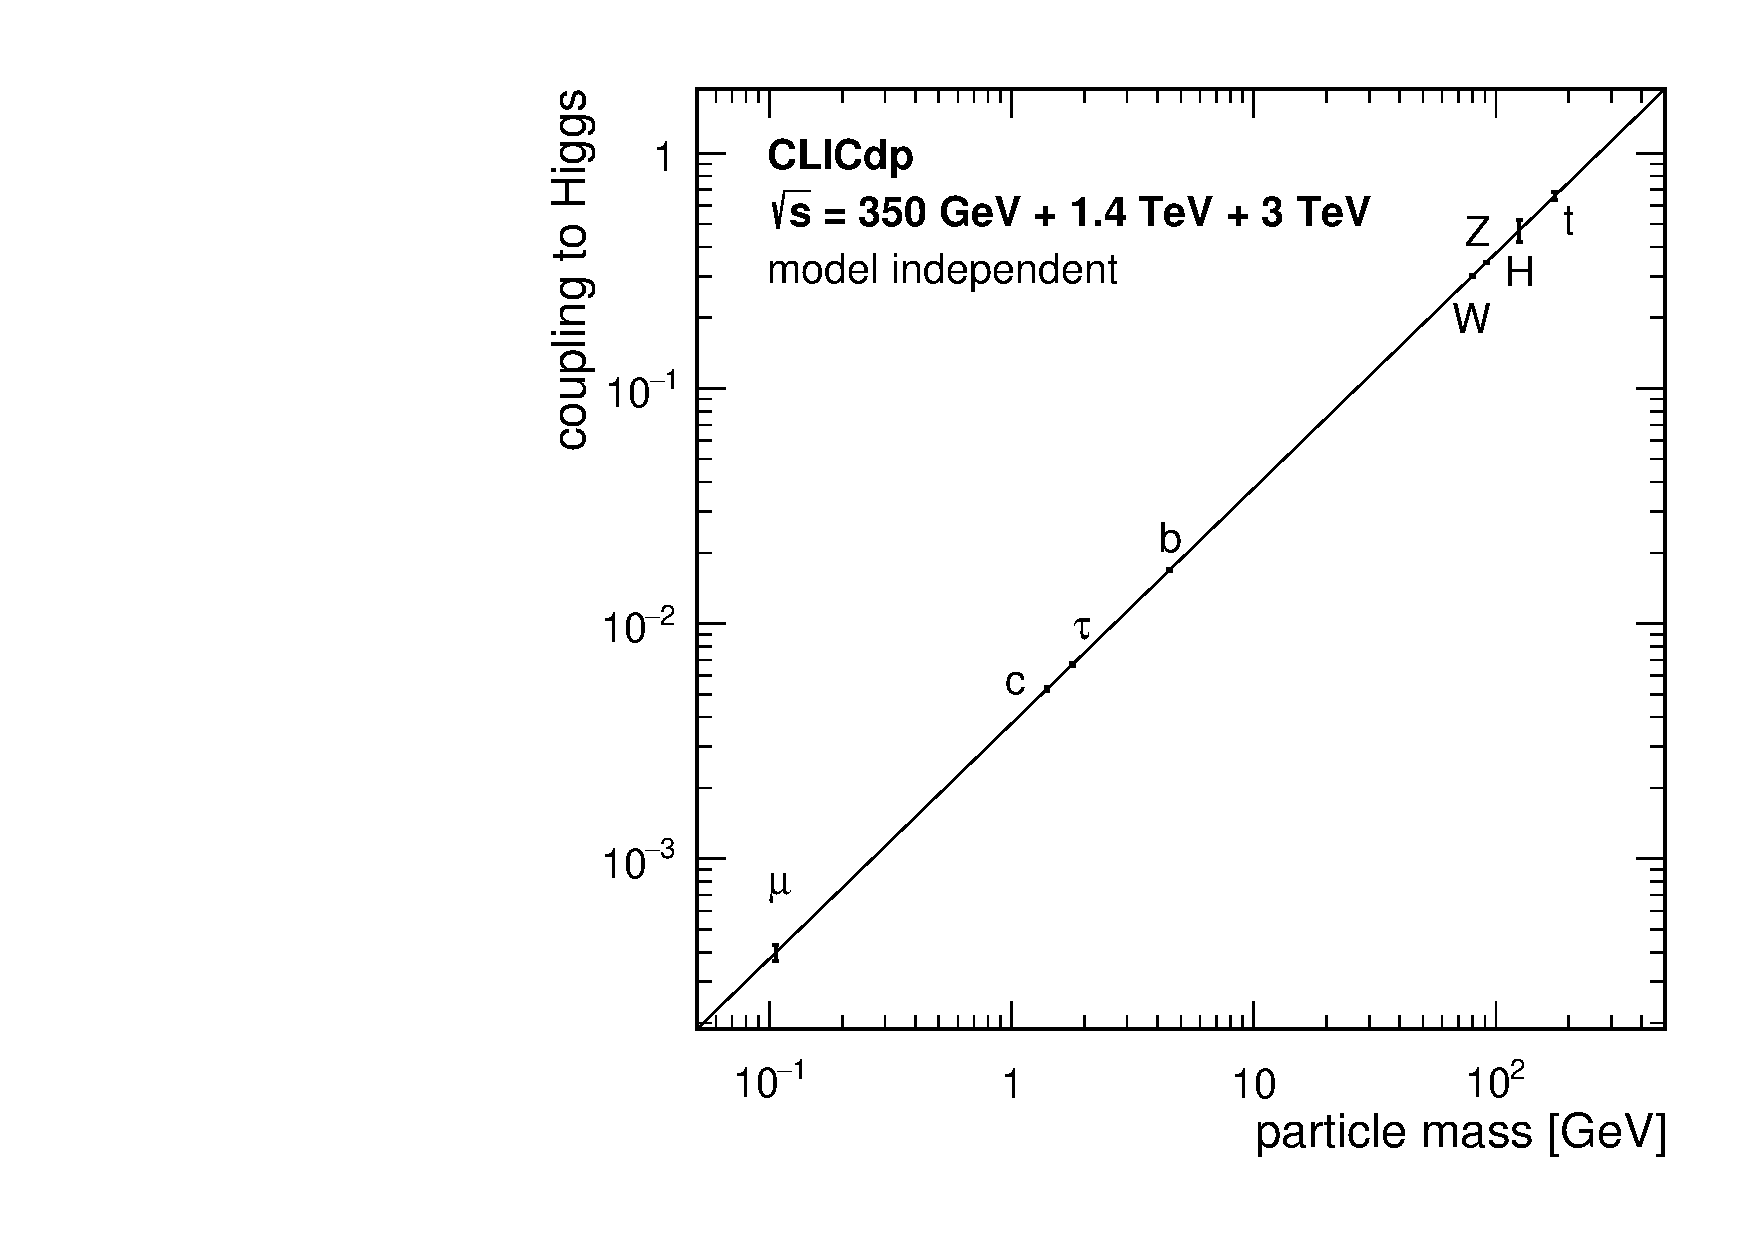
\includegraphics[width=0.95\linewidth]{Theory/fig/CouplingvsMassMI.pdf}
  \end{subfigure}
    \caption[Expected precision on model independent measurements of the Higgs couplings]{Expected precision on model independent measurements of the Higgs couplings \cite{Abramowicz:2016zbo}.}
  \label{fig:modelIndependentCouplings}
\end{figure}

\begin{figure}
\centering
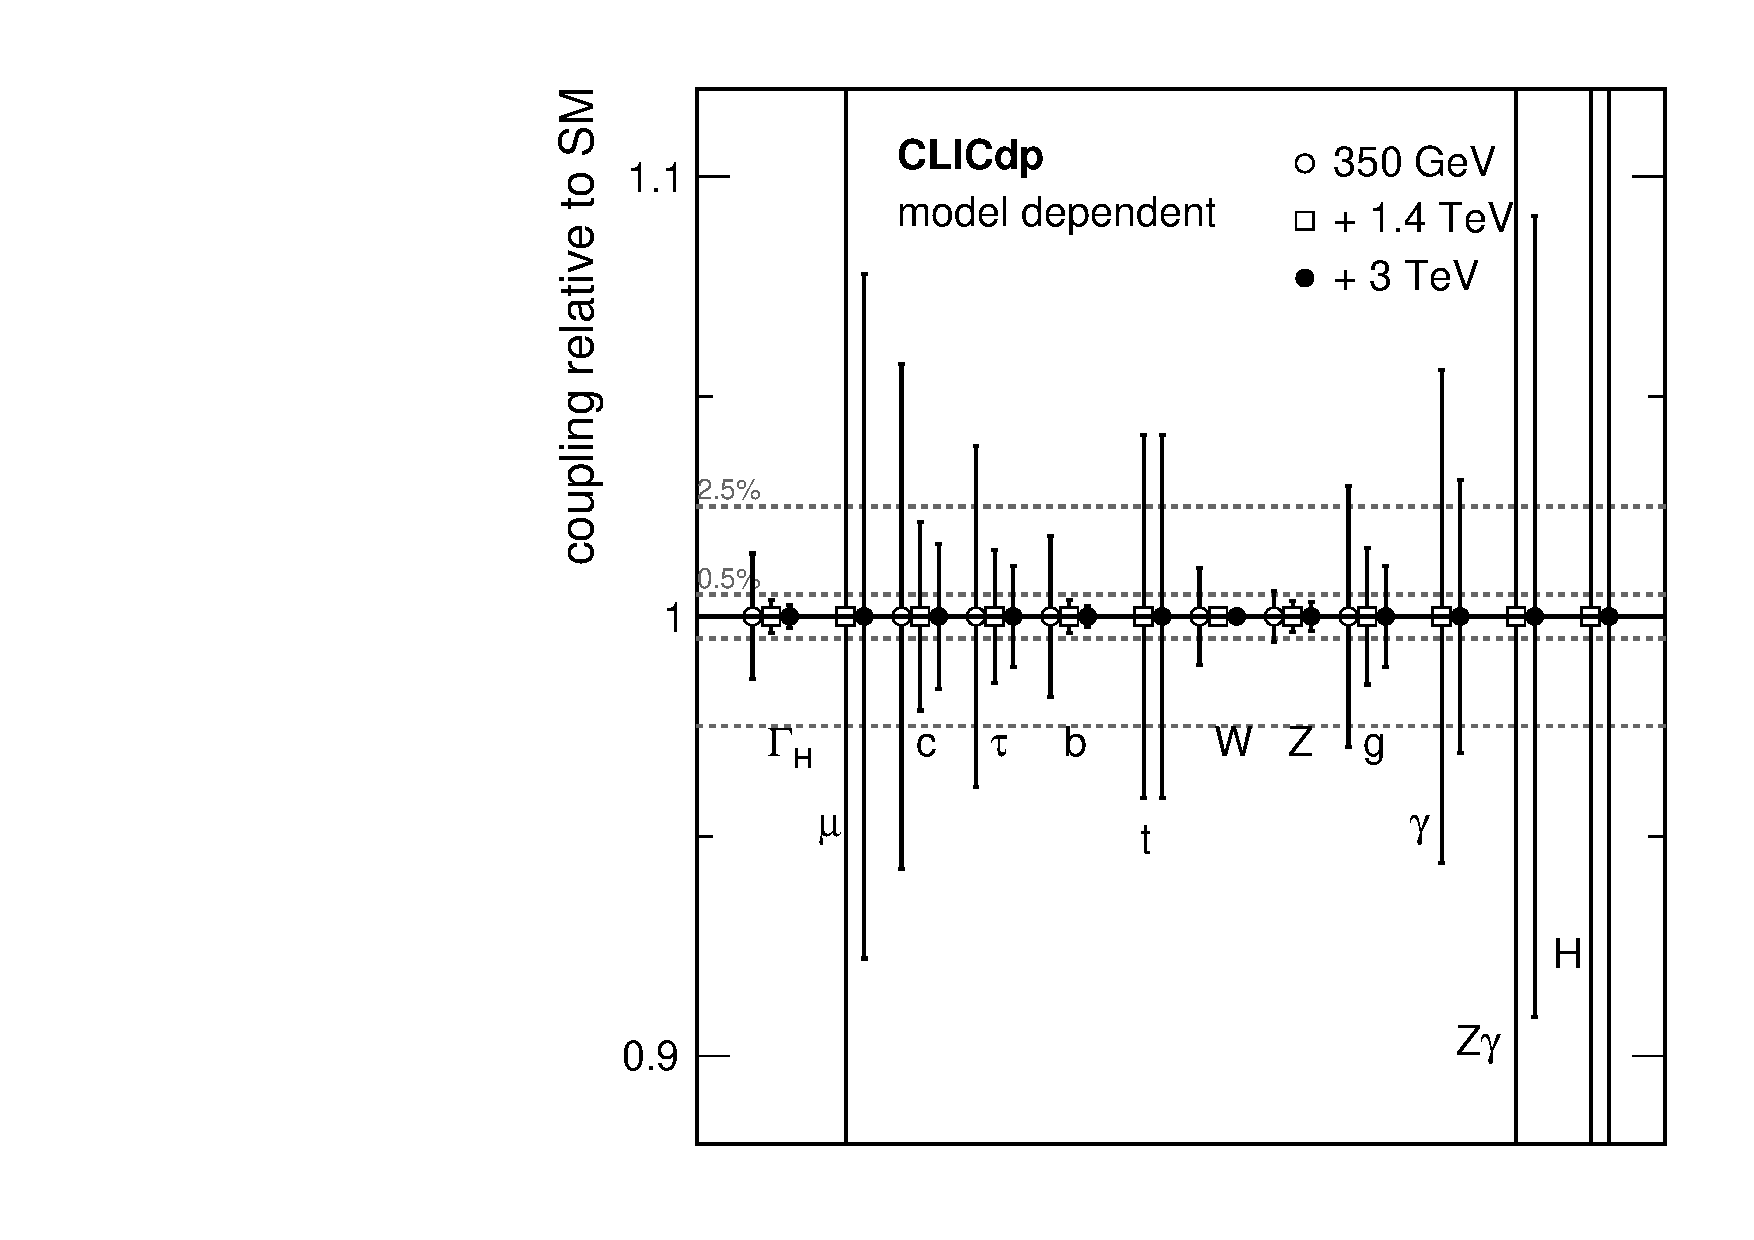
\includegraphics[width=0.65\linewidth]{Theory/fig/FitResultsMD.pdf}
\caption[Expected precision on model dependent measurements of the Higgs couplings at CLIC]{Expected precision on model dependent measurements of the Higgs couplings at CLIC \cite{Abramowicz:2016zbo}.}
\label{fig:modelDependentCouplings}
\end{figure}

\begin{figure}
\centering
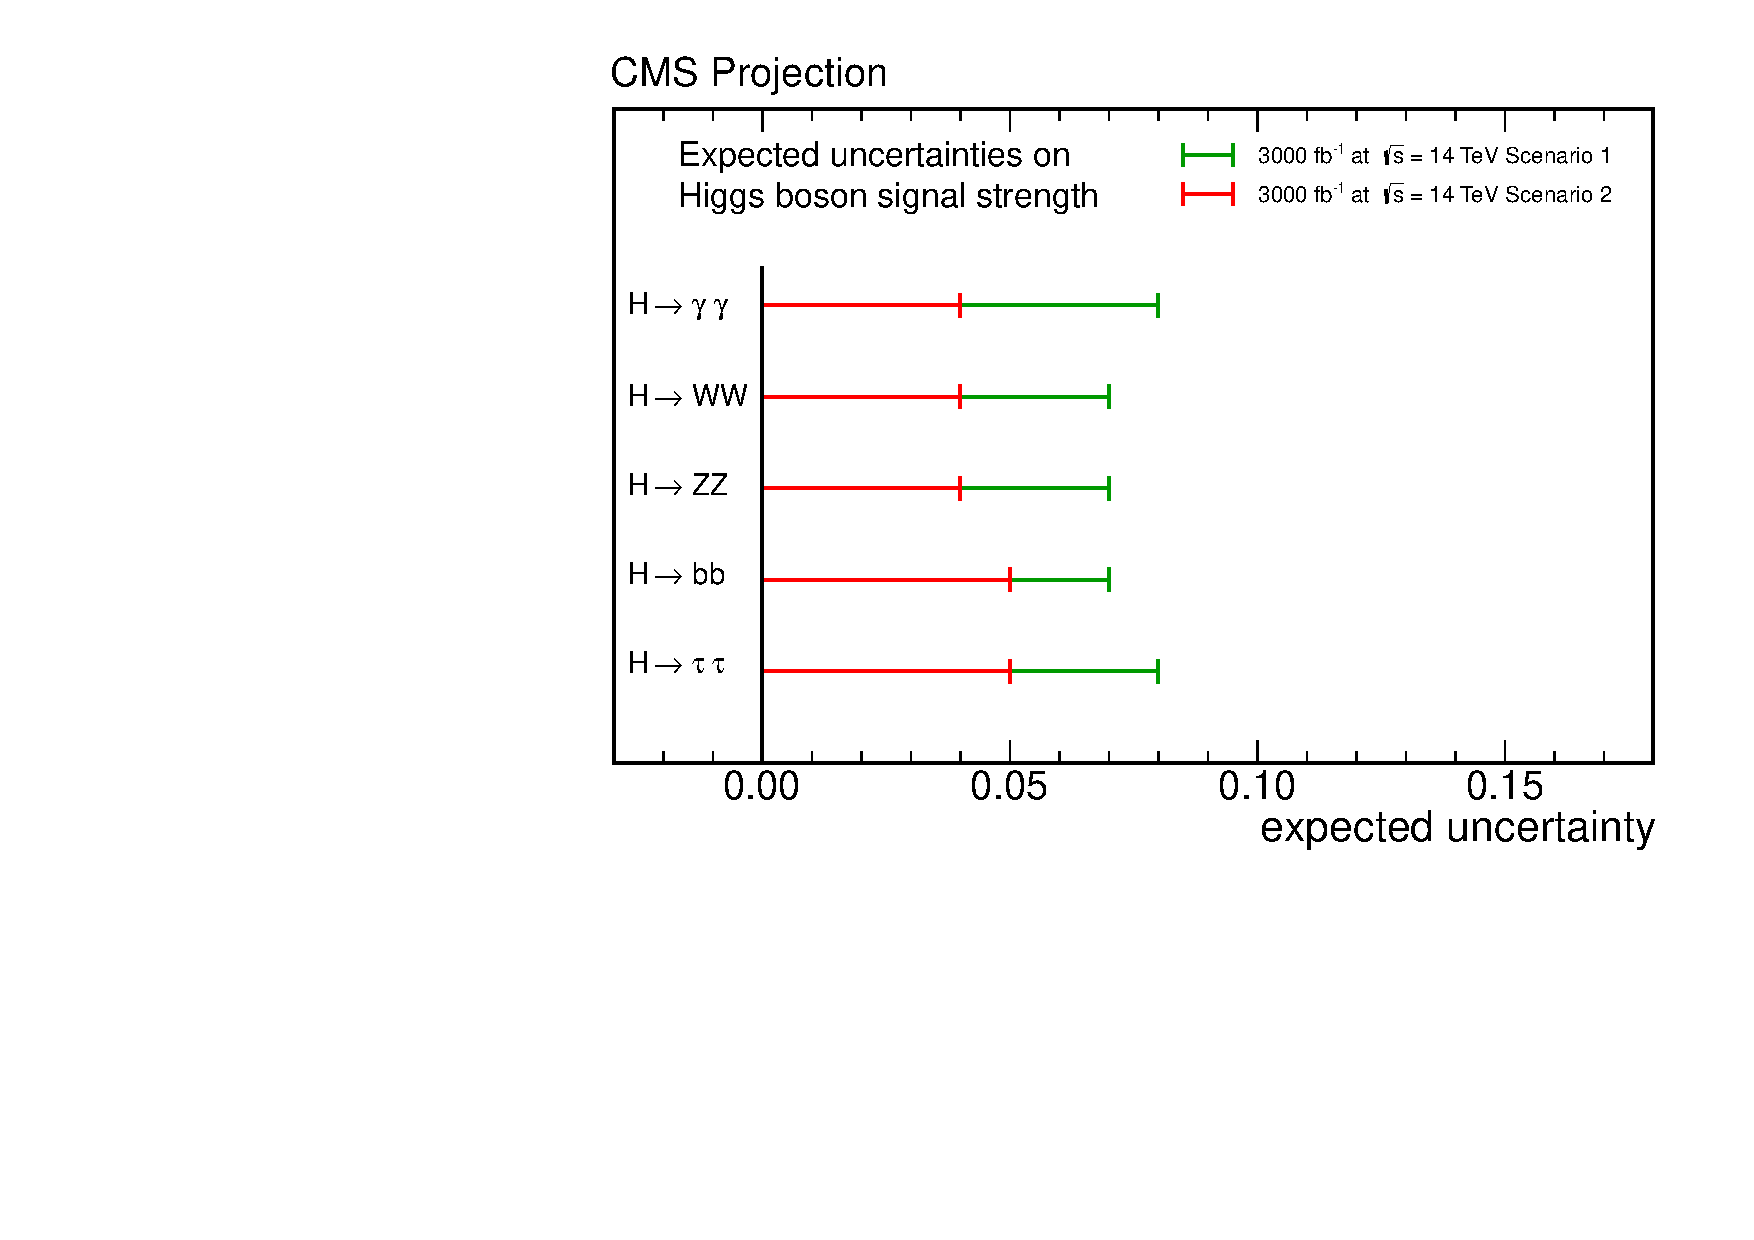
\includegraphics[width=0.7\linewidth]{Theory/fig/MuSnowmass3000.pdf}
\caption[Expected precision on model dependent measurements of the Higgs couplings at CMS]{Expected precision on model dependent measurements of the Higgs couplings at \ac{CMS} for the \ac{HL-LHC}. Scenario 1 represents a case where the systematic and theoretical uncertainties remain at their current levels. In scenario 2 the theoretical uncertainty is scaled by a factor of a half and the systematic uncertainties are scaled by the square root of the integrated luminosity \cite{CMS:2013xfa}.}
\label{fig:CMSHiggsPredictions}
\end{figure}

In practice it is expected that an 11 parameter global fit to multiple variations of these measurements will be performed at each stage of operation to extract the Higgs width and its couplings to both fermions and bosons. The relevant inputs for these fits are shown in \reftab{fig:350GeVNumbers} and \ref{fig:HighENumbers} while the results of the fits are shown in \reffig{fig:modelIndependentCouplings}.

For context it is also important to compare these results to what can be expected from experiments such as ATLAS and CMS at the LHC. Because the Higgs width can not be explicitly calculated at hadron colliders, it is appropriate to compare the model dependent version of the CLIC analysis with those predicted by ATLAS and CMS. In this situation, because the precision of the couplings is no longer limited by the precision on $g_{HZZ}$, the predicted precision for CLIC is seen to improve considerably. One can see from \reffig{fig:modelDependentCouplings} and \ref{fig:CMSHiggsPredictions} that in many cases CLIC is expected to provide an order of magnitude improvement over what can be achieved at the LHC with many of the key parameters associated with the Higgs being measured to sub percent precision.

Ultimately the aim of performing precision measurements is to allow the validation or rejection of theoretical models. While the results seen so far at the LHC suggest that the observed Higgs boson is that of the \ac{SM}, there are numerous alternative theories that predict a Higgs like particle with properties similar to what has been observed but which differ to a degree not yet measurable by current experiments. The details of these theories will not be expanded upon within this thesis, however the deviations expected in the Higgs couplings of these theories relative to the \ac{SM} are shown in \reftab{table:snowmass}. These values should only be taken as a rough guideline for the precision required to discover/reject the theories as they are based on the assumption that new physics occurs at a specific scale (in this case 1~TeV). Although the precision required to provide sensitivity to these models is expected to be greater than that expected for the LHC, it may be within the scope of the proposed CLIC physics programme.  

\begin{table}
  \centering
  \begin{tabular}{l c c c}
    \toprule
    \toprule
    Model  & $\kappa_V$ & $\kappa_b$ & $\kappa_\gamma$  \\
    \midrule
    Singlet Mixing & $\sim$6\% & $\sim$6\%  & $\sim$6\% \\
    2HDM & $\sim$1\% & $\sim$10\%  & $\sim$1\% \\
    Decoupling MSSM & $\sim$-0.0013\% & $\sim$1.6\%  & $\sim$-.4\% \\
    Composite & $\sim$-3\% & $\sim$-(3-9)\%  & $\sim$-9\% \\
    Top Partner & $\sim$-2\% & $\sim$-2\%  & $\sim$+1\% \\
    \bottomrule
    \bottomrule
  \end{tabular}
  \caption[Predicted Higgs Coupling Modifications for BSM theories]{Generic size of Higgs coupling modifications from the \ac{SM} values when all new particles are $M\sim 1 TeV$ and mixing angle satisfy precision electroweak fits. The decoupling MSSM numbers assume $\tan\beta = 3.2$ and a stop mass of 1 TeV with $X_t =0$ for the $\kappa_\gamma$ prediction \cite{Dawson:2013bba}. $\kappa_{V,b,\gamma}$ denote the model dependent couplings of the vector bosons, b quark and photon to the Higgs.}
  \label{table:snowmass}
\end{table}

\section{Top Quark Physics}


The top quark is currently the heaviest particle within the \ac{SM} and is the only quark that decays before undergoing hadronization. Due to its high mass, top interactions are good channels for looking for \ac{BSM} physics with a characteristic energy scale beyond what has currently been discovered. Due to its high mass, the top is also the fermion with the strongest coupling to the Higgs making it a good candidate for finding deviations from the \ac{SM} within the Higgs sector. As such, the physics programme for \ac{CLIC} will measure the top quark's properties during the lowest energy stage of operation featuring a dedicated top threshold scan aiming to provide precision measurements of the top mass and width. The dominant production mechanism for top production is through the $s$-channel: $e^+e^-\rightarrow\gamma /Z\rightarrow t\bar{t}$ process shown in \reffig{fig:topFeynmann}. Using this process the properties of the $t\bar{t}\gamma$ and $t\bar{t}Z$ vertices can be measured. Examining these can provide sensitivity to contributions from \ac{BSM} effects such as the existence of extra bosons (e.g. $Z'$ \cite{Langacker:2008yv}) which could provide an additional production channel, modifying the behavior at the vertex. The  $t\bar{t}X$ vertex can be written as\cite{Amjad:2015mma}

\begin{figure}
\centering
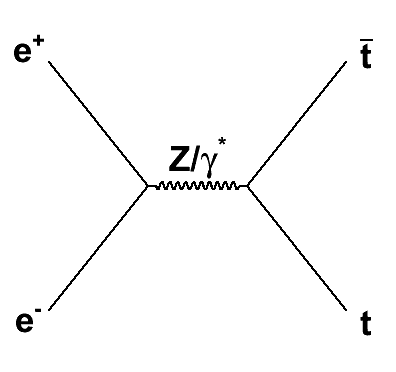
\includegraphics[width=0.35\linewidth]{Theory/fig/ttFeynmann}
\caption[Dominant top production mechanism at electron positron colliders]{Dominant top production mechanism at electron positron collider}
\label{fig:topFeynmann}
\end{figure}

\begin{equation}
\Gamma_{\mu}^{t\bar{t}X}(s,q,\bar{q})= ie\{ \gamma_{\mu}(F_{1V}^{X}(s)+ \gamma_{5}F_{1A}^{X}(s)) - \frac{\sigma_{\mu\nu}}{2m_t}(q+\bar{q})^{\nu}(iF_{2V}^{X}(s) + \gamma_{5}F_{2A}^{X}(s))\},
\end{equation}

where $X=\gamma /Z$, $q$ and $\bar{q}$ are the four momenta of the top and anti top, $s$ is $(q+\bar{q})^2$, $\gamma_\mu$ and $\gamma_\mu\gamma_5$ are the Dirac matrices corresponding to vector and axial-vector currents respectively, $\sigma_{\mu\nu}=\frac{i}{2}(\gamma_\mu \gamma_\nu -\gamma_\nu \gamma_\mu)$ allows for describing the scattering and $F$ are the electroweak form factors. Within the \ac{SM}, the only non-zero form factors at tree level are

\begin{equation}
F_{1V}^{\gamma}=\frac{2}{3},
\end{equation}

\begin{equation}
F_{1V}^{Z}=\frac{1}{4\sin\theta_{W}\cos\theta_{W}}(1-\frac{8}{3}\sin\theta_{W}),
\end{equation}

\begin{equation}
F_{1A}^{Z}=\frac{1}{4\sin\theta_{W}\cos\theta_{W}},
\end{equation}

where $\theta_W$ is the weak mixing angle. While the remaining form factors ($F_2$ and $F_{1A}^{\gamma}$) are predicted to be zero up to three-loop level in the \ac{SM}, several \ac{BSM} models predict they can gain a non-zero contribution at the one-loop level\cite{Abe:2001swa} making them a useful tool for probing the \ac{SM}. Combinations of these factors can be related to physical observables which can be measured at CLIC. The couplings of the bosons to quarks with left or right handed helicity can be expressed as

\begin{equation}
g_L^X = F_{1V}^{X} - F_{1A}^{X} ~~~~~~~~~~~ g_R^X = F_{1V}^{X} + F_{1A}^{X}
\end{equation}

The most directly observable experimental variables are the total cross section and the forward backward asymmetry (\afb). These are the measurements that are presented later within this thesis and will be discussed in more detail in Chapter \ref{chapter:topanalysis}. The forward backward asymmetry is of special interest as the measurement of the b quark forward-backward asymmetry at \ac{LEP}\cite{ABBIENDI200229} currently produces the largest tension with the \ac{SM}, $\mathcal{O}(3\sigma)$\cite{ALEPH:2005ab}, in electroweak fits. These variables are found to be dependent on the helicity of the incoming electrons \cite{Schmidt:1995mr} and so are more easily expressed in terms of the alternative form factors:

\begin{equation}
F_{ij}^{L} = -F_{ij}^{\gamma} +(\frac{-\frac{1}{2} +\sin\theta_W^2}{\sin\theta_W\cos\theta_W})(\frac{s}{s-m_Z^2}) -F_{ij}^{Z},
\end{equation}

\begin{equation}
F_{ij}^{R} = -F_{ij}^{\gamma} +(\frac{\sin\theta_W^2}{\sin\theta_W\cos\theta_W})(\frac{s}{s-m_Z^2}) -F_{ij}^{Z},
\end{equation}

where $L$,$R$ represent the polarization of the electron, $i$=1,2 and $j$=$V$,$A$. In this notation, for an electron polarization P, the total $ee\rightarrow Z/\gamma\rightarrow tt$ cross section and \afb can be expressed as:

\begin{equation}
\sigma_P = \frac{8\pi\alpha(s)^2}{s}\beta \{(1 + \frac{1}{2\gamma^2})(F_{1V}^P)^2 +(\beta F_{1A}^P)^2 +3F_{1V}^P F_{2V}^P + (1 + \frac{1}{2\gamma^2})(F_{2V}^P)^2\},
\end{equation}

\begin{equation}
\label{eq:afbFormFactors}
A_{FB}(P) = \mp \frac{12\pi\alpha(s)^2 \beta^2}{s}\frac{F_{1A}^P(F_{1V}^P +F_{2V}^P)}{\sigma_P},
\end{equation}

where $\alpha(s)$  is the electromagnetic coupling, $\gamma$ and $\beta$ are the Lorentz factor and speed of the top, and for \refeq{eq:afbFormFactors}, the $+$ and $-$ refer to the $P=R$ and $P=L$ cases respectively. A single measurement of the cross section and \afb alone would not allow the form factors to be determined because the system would be underconstrained. However, because the cross section and \afb vary with $\beta$, $\gamma$ and $P$, then by performing the measurement at multiple energies and making use of the fact that \ac{CLIC} can be operated with different beam polarizations, it becomes possible to extract all relevant couplings. An example of how \afb varies with the centre-of-mass of the collision, $\sqrt{s}$, for a fixed polarization is shown in \reffig{fig:AfbSDependence}, while the cross section dependence is shown in \reffig{Fig:SuperSym}. The only exceptions to this are the $F_{2A}^X$ factors which do not affect these two variables and so must be measured using alternative methods. 

\begin{figure}
  \centering
  \includegraphics[width=0.65\textwidth]{TopAnalysis/figures/asym-top.eps}
  \caption[Predicted forward backward asymmetry as a function of collision energy]{Predicted forward backward asymmetry as a function of collision energy\cite{Fleischer:2003kk}.}
  \label{fig:AfbSDependence}
\end{figure}

\begin{figure}
\centering
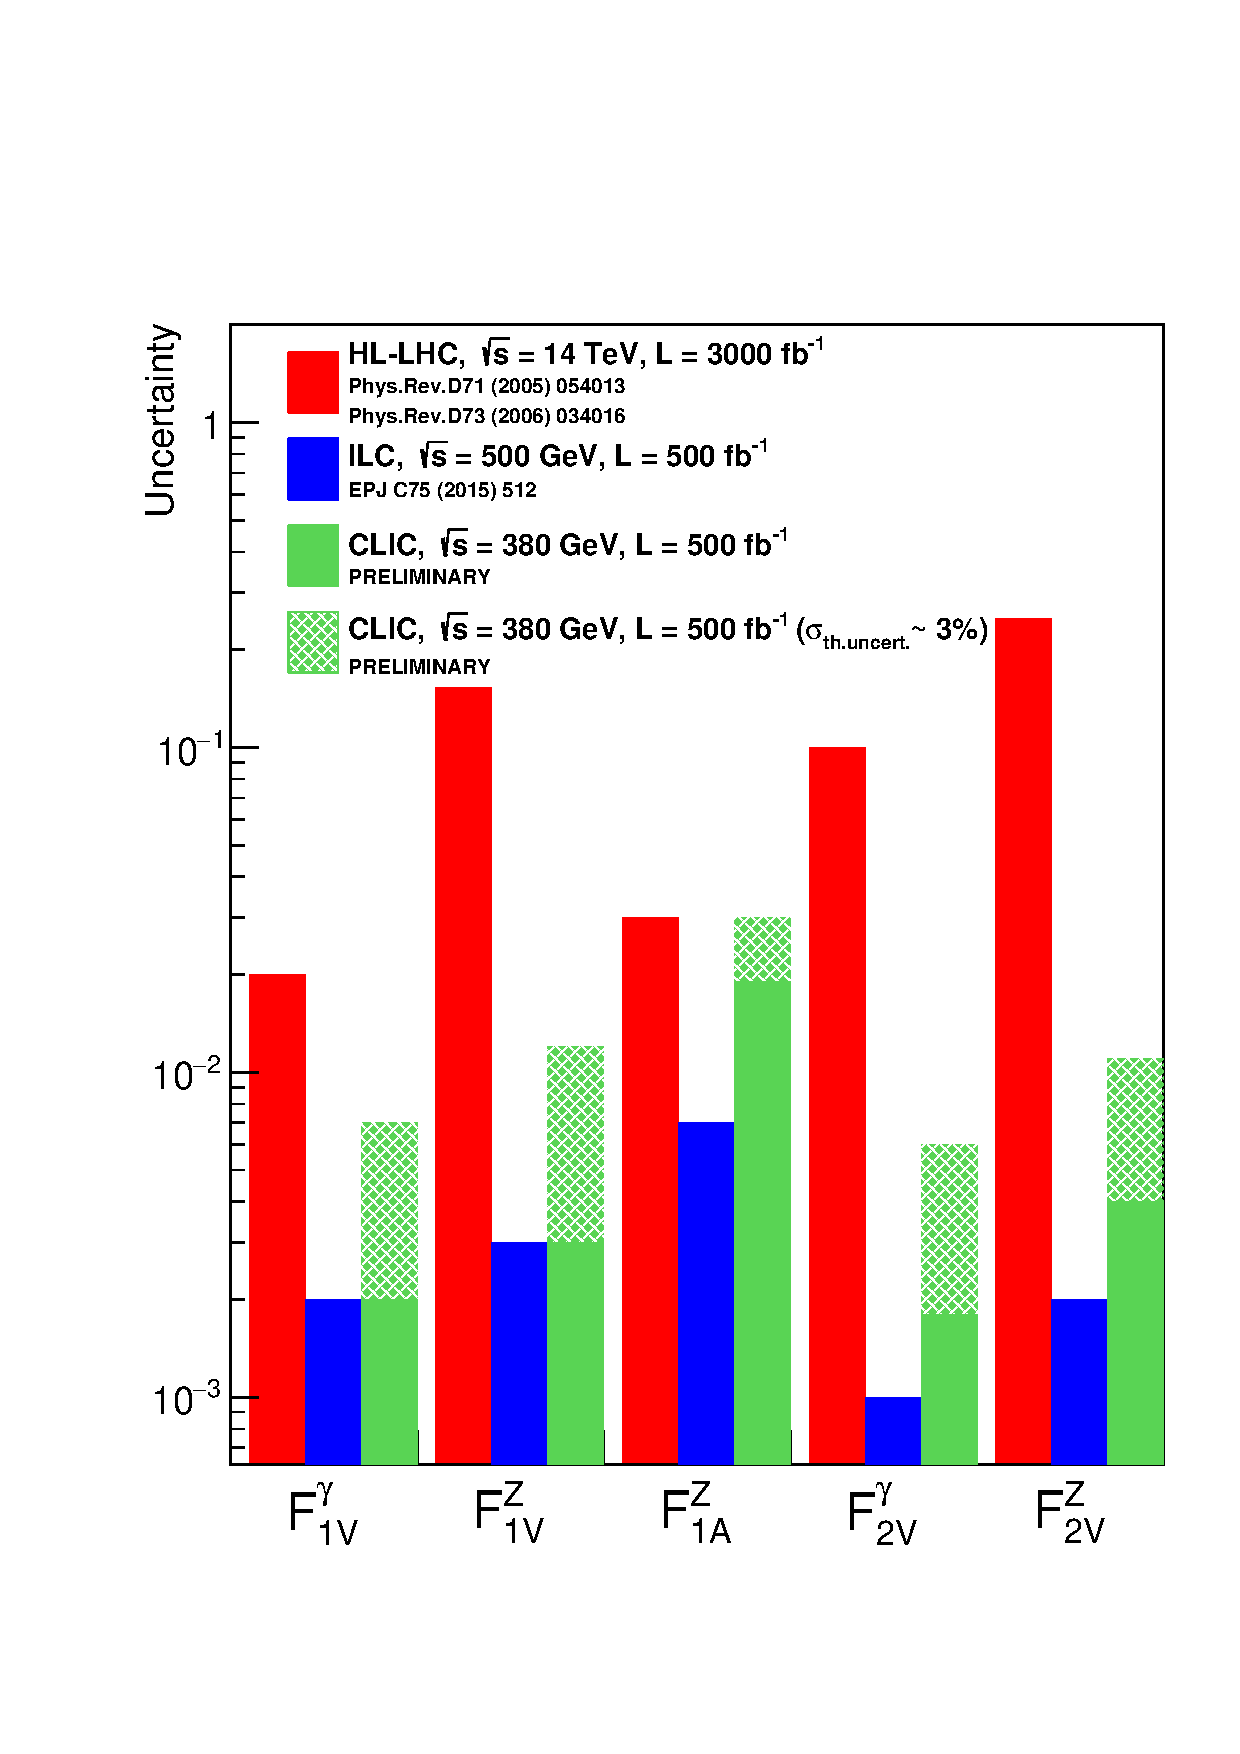
\includegraphics[width=0.65\linewidth]{Theory/fig/FormFactorsTopCLIC380.pdf}
\caption[Expected precision on CP conserving electroweak form factors at future colliders]{Expected precision on CP conserving electroweak form factors at future colliders \cite{CLIC:2016zwp}}
\label{fig:CPConserving}
\end{figure}

The predicted uncertainty with which the couplings are expected to be measured at \ac{CLIC} based on generator level studies, as well as the equivalent results for \ac{ILC} and \ac{HL-LHC}, is shown in \reffig{fig:CPConserving}. The expected precision from performing these measurements at a lepton collider is an order of magnitude better than that expected from hadron colliders. Overall there will be more tops produced in a hadron collider, however the production mechanisms are often more complicated making it harder to extract the couplings. As a result the form factors will usually be extracted from ttZ and tt$\gamma$ final states rather than s-channel production\cite{Baur:2005wi} which makes them harder to relate to observables such as \afb. It is also harder to identify tops (which typically decay to at least one jet) in an environment that contains \ac{QCD} jets from beam remnants compared to at lepton colliders where there is minimal \ac{QCD} background within an event.

\chapter{Higgs to WW$^*$ at 1.4 TeV}
\label{Higgs Analysis}

\begin{figure}
  \centering
  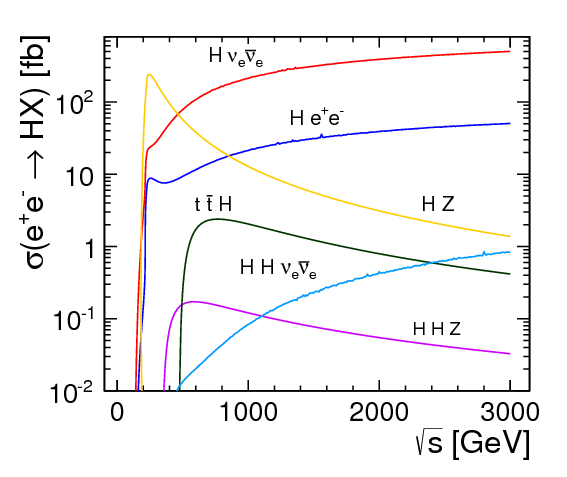
\includegraphics[width=0.7\textwidth,keepaspectratio]{Theory/fig/HiggsCrossSections}
  \caption[Cross Sections For Higgs Production Mechanisms]{Cross sections for dominant Higgs production mechanisms as a function of energy \cite{Abramowicz:2016zbo}. Higgs production via WW-fusion is shown in red.}
  \label{fig:higgsXSecs2}
\end{figure}

As mentioned in Chapter \ref{theory}, one of the key aims of the \ac{CLIC} physics programme will be to perform model independent measurements of the Higgs couplings. In order to be able to do this, the total width of the Higgs must first be measured. This has been found to be possible by taking the ratio of four different measurements:


\hspace{120pt}  $X_1=\sigma_{ZH} \propto g_{HZZ}^2$

\hspace{120pt}   $X_2=\sigma_{H\nu\bar{\nu}} \times BR(H\rightarrow WW^*) \propto \frac{g_{HWW}^4}{\Gamma_H}$

\hspace{120pt}   $X_3=\sigma_{H\nu\bar{\nu}} \times BR(H\rightarrow b\bar{b}) \propto \frac{g_{HWW}^{2}g_{Hbb}^2}{\Gamma_H}$

\hspace{120pt}   $X_4=\sigma_{ZH} \times BR(H\rightarrow b\bar{b}) \propto \frac{g_{HZZ}^{2}g_{Hbb}^2}{\Gamma_H}$


Here we will look at the measurement of one of these, $X_2$. As can be seen from \reffig{fig:higgsXSecs2}, WW-fusion is the dominant Higgs production mechanism for energies above $\sim $500 GeV and so this measurement is best performed in the higher energy stages of operation. In particluar we will focus on measuring $X_2$ at 1.4 TeV. For measuring the branching ratio of H$\rightarrow$WW$^*$ there are three potential final states that can be examined depending on the decay mode of the two W's. An individual W will decay hadronically (into a quark pair) 67.41\% of the time and leptonically (into a lepton + neutrino) 32.58\% of the time.  The combinations available from each W decay gives three final states referred to as the hadronic, semileptonic and leptonic decay modes corresponding to both W's decaying hadronically, one W decaying hadronically while the other decays leptonically and both W's decaying leptonically respectively. The relative abundance for each decay mode is roughly 4:4:1. Here we will only study the semileptonic mode (\reffig{fig:semileptonic}.) An equivalent analysis has already been performed for the hadronic decay mode yielding a statistical precision of 1.5\% on $X_2$ \cite{Abramowicz:2016zbo}. Due to it's lower branching ratio, the leptonic decay mode has yet to be studied as it is not expected to yield a significant improvement on the statistical precision achievable for $X_2$. 

\begin{figure}
  \centering
  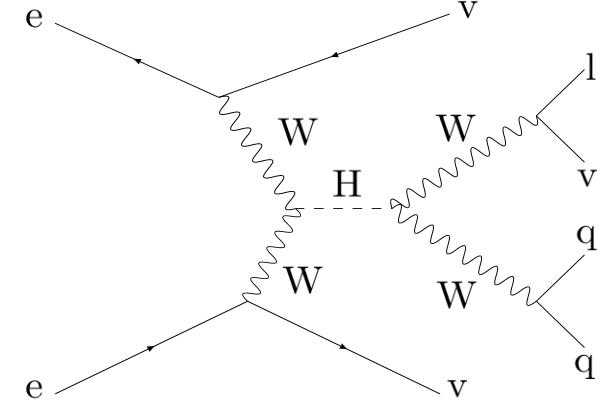
\includegraphics[width=0.7\textwidth,keepaspectratio]{Experiments/fig/feynmann}
  \caption[Semileptonic decay channel for  WW$^*$ decays of Higgs produced through WW-fusion]{Semileptonic decay channel for  WW$^*$ decays of Higgs produced through WW-fusion.}
  \label{fig:semileptonic}
\end{figure}

\section{Event Generation}

All events used in this analysis were produced centrally by \ac{CLIC} using WHIZARD 1.95 \cite{Kilian:2007gr} and are summarised in \reftab{fig:higgsbackgrounds}. In the case of $e\gamma$ events, a scale factor of 2 was applied to the cross section to account for interactions occuring with both the electron and positron. In the case of beamsstrahlung events (simulated using GUINEA-PIG \cite{Schulte:382453}), a further scaling of 0.75 was applied to account for the lower luminosity of these type of collisions. Sample 2022 is the $ee\rightarrow H\nu\nu$ inclusive sample. The relevant events were extracted from this main sample by performing a parton level event selection to identify events in which the Higgs decayed to W's and separating these according to their decay products. At this point events in which the lepton produced in the W decay is found to be a tau are excluded from the signal defintion due to the fact they produce a different topology in the final state compared to electrons and muons. In all cases the detector model used is CLIC\_ILD\_CDR, CLIC's variation of the ILD detector designed for ILC described in the \ac{CLIC} CDR\cite{CDR}. The main backgrounds of note are: ee$\rightarrow$qql$\nu$ (dominated by e$^+$e$^-\rightarrow$W$^+$W$^-$) as it has a very similar topology to the signal process and so is expected to be the most difficult to exclude; and ee$\rightarrow$ H(WW$^*\rightarrow$qqqq)$\nu\nu$ as contamination from these events after event selection must be taken into account before any combination of results from the semileptonic and hadronic channels can be made.


\begin{figure}
  \centering
  \begin{tabular}{l r r r}
   \toprule
    Process     & Cross Section(fb)  &   Production ID\cite{bib-prodids}    & Events Used    \\
    \midrule
    Signal: ee$\rightarrow$ H(WW$^*\rightarrow$qql$\nu$)$\nu\nu$             &   17.3  &  2022  & 70000  \\ 
    \midrule
    ee$\rightarrow$ H(WW$^*\rightarrow$qqqq)$\nu\nu$                &   27.4  &  2022    & 100000 \\
    \midrule
    ee$\rightarrow$ H$^*\rightarrow$ Other & 199.4 & 2022 & 800000  \\
    \midrule
    ee$\rightarrow$qq               & 4009.5    &  2091  & 500000  \\ 
    \midrule
    ee$\rightarrow$qqqq               & 1328.1    &  2163  & 300000  \\ 
    \midrule
    e$\gamma$$\rightarrow$eqq ($\gamma$ from EPA)                 & 32308    &  2515 & 500000   \\ 
    \midrule
    e$\gamma$$\rightarrow$eqq ($\gamma$ from BS)               & 56043  &  2527  & 500000 \\ 
    \midrule
    ee$\rightarrow$qq$\nu\nu$               & 787.7    &  3243 & 500000   \\ 
    \midrule
    ee$\rightarrow$qqll               & 2725.8    &  3246  & 400000  \\ 
    \midrule
    ee$\rightarrow$qql$\nu$              & 4309.7    &  3249 & 1000000   \\ 
    \bottomrule
  \end{tabular}
  \caption[Samples used for the H$\rightarrow$WW$^*$ analysis]{Samples used for the H$\rightarrow$WW$^*$ analysis}
  \label{fig:higgsbackgrounds}
\end{figure}


\section{Event Reconstruction}

Reconstruction of the signal events was performed using ILCSOFT v01-17-06 and was carried out in two main stages as described below. The first stage was to identify the isolated lepton associated with the leptonic W boson decay. The second stage involved removing this isolated lepton and resolving the remaining particles into two jets that were associated with the two quarks produced by the hadronically decaying W boson. Using the two jets, the W boson could then be reconstructed and combined with the isolated lepton to reconstruct the Higgs boson. The reconstructed Higgs candidate will not be complete due to the missing energy and momentum  from the lepton neutrino produced from the W decay. However, the observed properties will still be sufficient for providing discrimination between signal and background events.

\subsection{Lepton Identification}
Two different methods were used for identifying leptons. The primary method for particle identification is to assume that the highest energy electron or muon (as identified by PandoraPFA \cite{Thomson200925}) corresponds to the isolated lepton from the leptonically decaying W boson. This method was found to have an efficiency of 93\% (90\% for electrons, 96\% for muons) and purity of 96\% for identifiying the isolated lepton. The improved efficiency for muons relative to electrons is a result of the different signatures they leave in the detector. Electrons are identified by the presence of a track followed by a deposit in the \ac{ECAL}. If the track is not reconstructed or is wrongly attributed to a different calorimeter deposit by Pandora, the electron will be wrongly identified as a photon (characterised by no track, only energy deposited in the \ac{ECAL}.) Muons on the other hand are highly penetrating and so leave deposits in the \ac{HCAL} and muon tail catchers as well as the tracker and \ac{ECAL}. As a result, even if one part of the detector system fails there is enough redundancy in the measurement that the muon should still be identified.

\begin{figure}
  \centering
  \begin{subfigure}[t]{.48\textwidth}
    \centering
    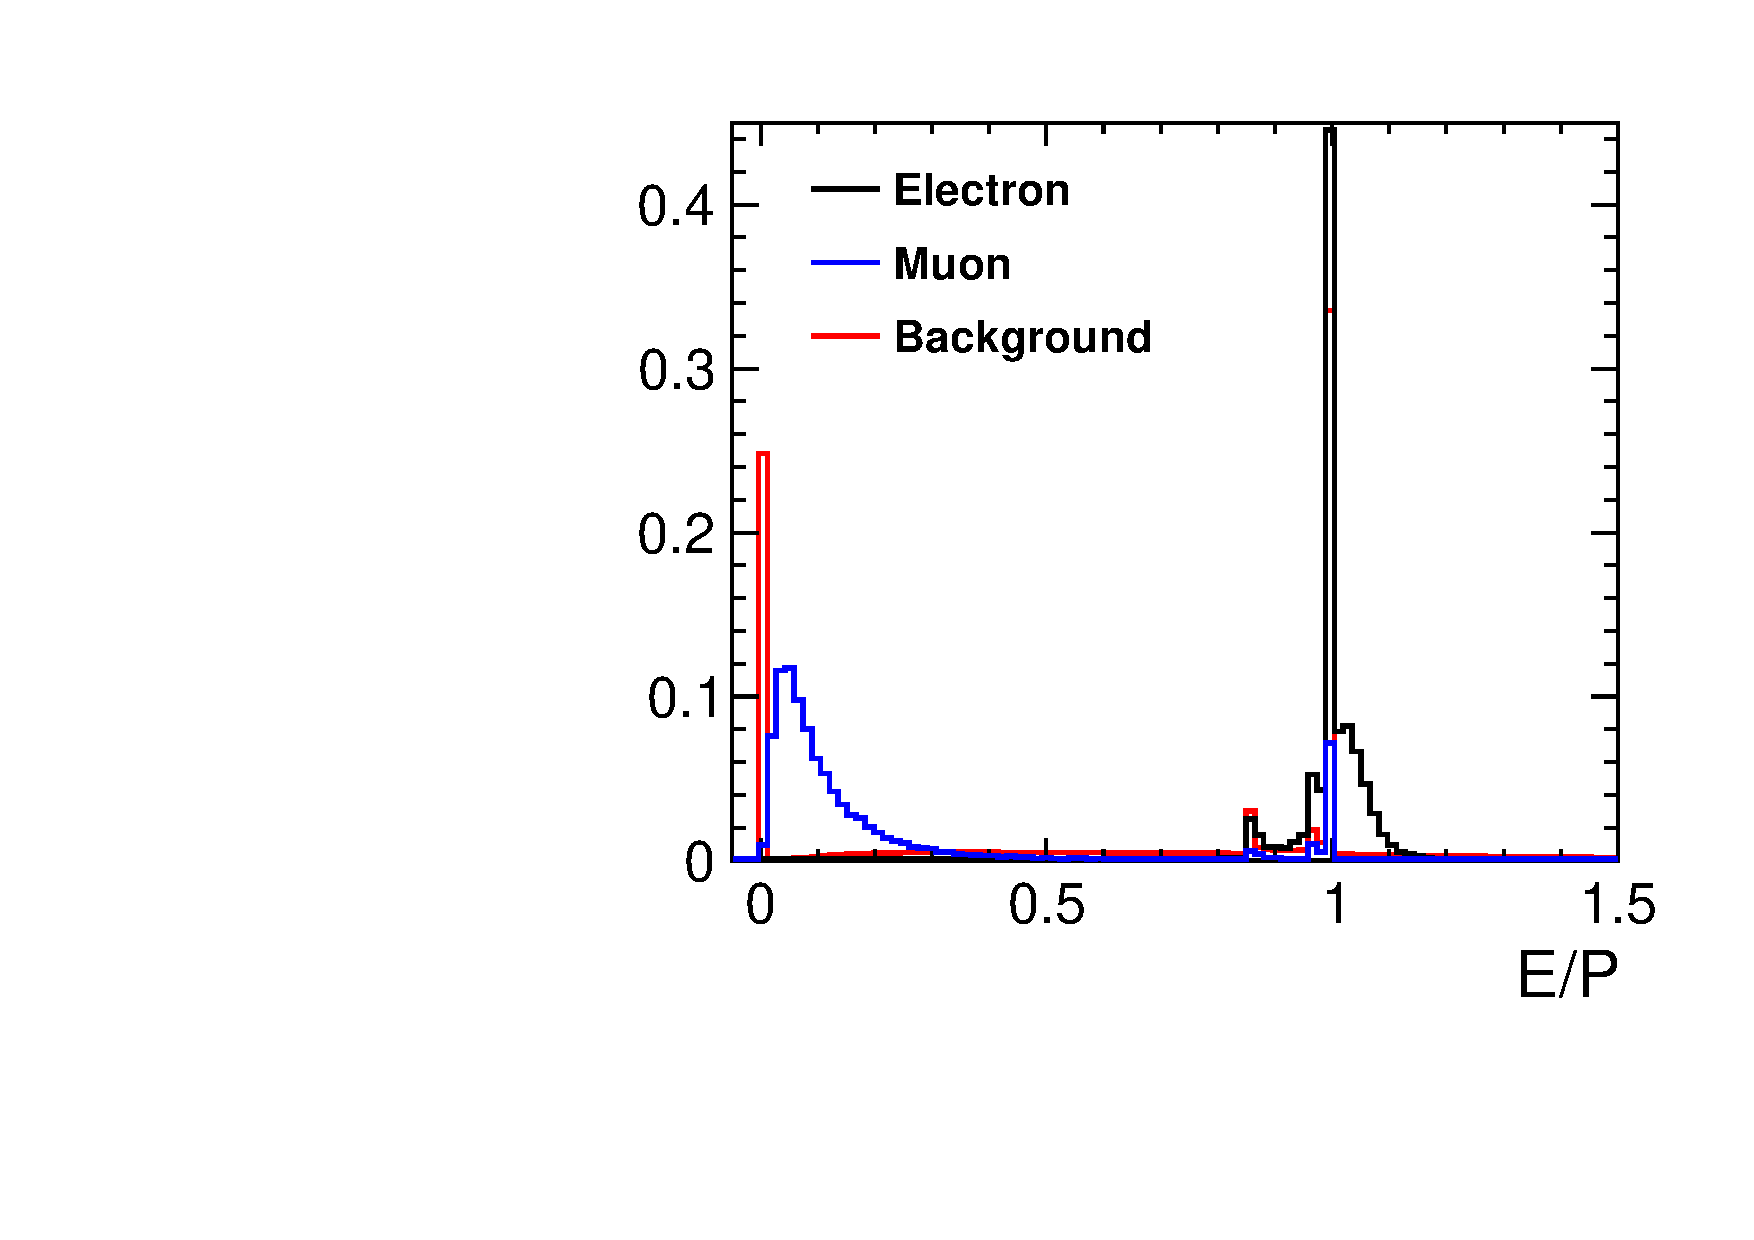
\includegraphics[width=1.0\linewidth,keepaspectratio]{HiggsAnalysis/figures/EByP}
    \caption{Ratio of the energy deposited in both calorimeters to the particles momentum.}
  \end{subfigure}%%
    \vspace{4ex}
  \begin{subfigure}[t]{.48\textwidth}
    \centering
    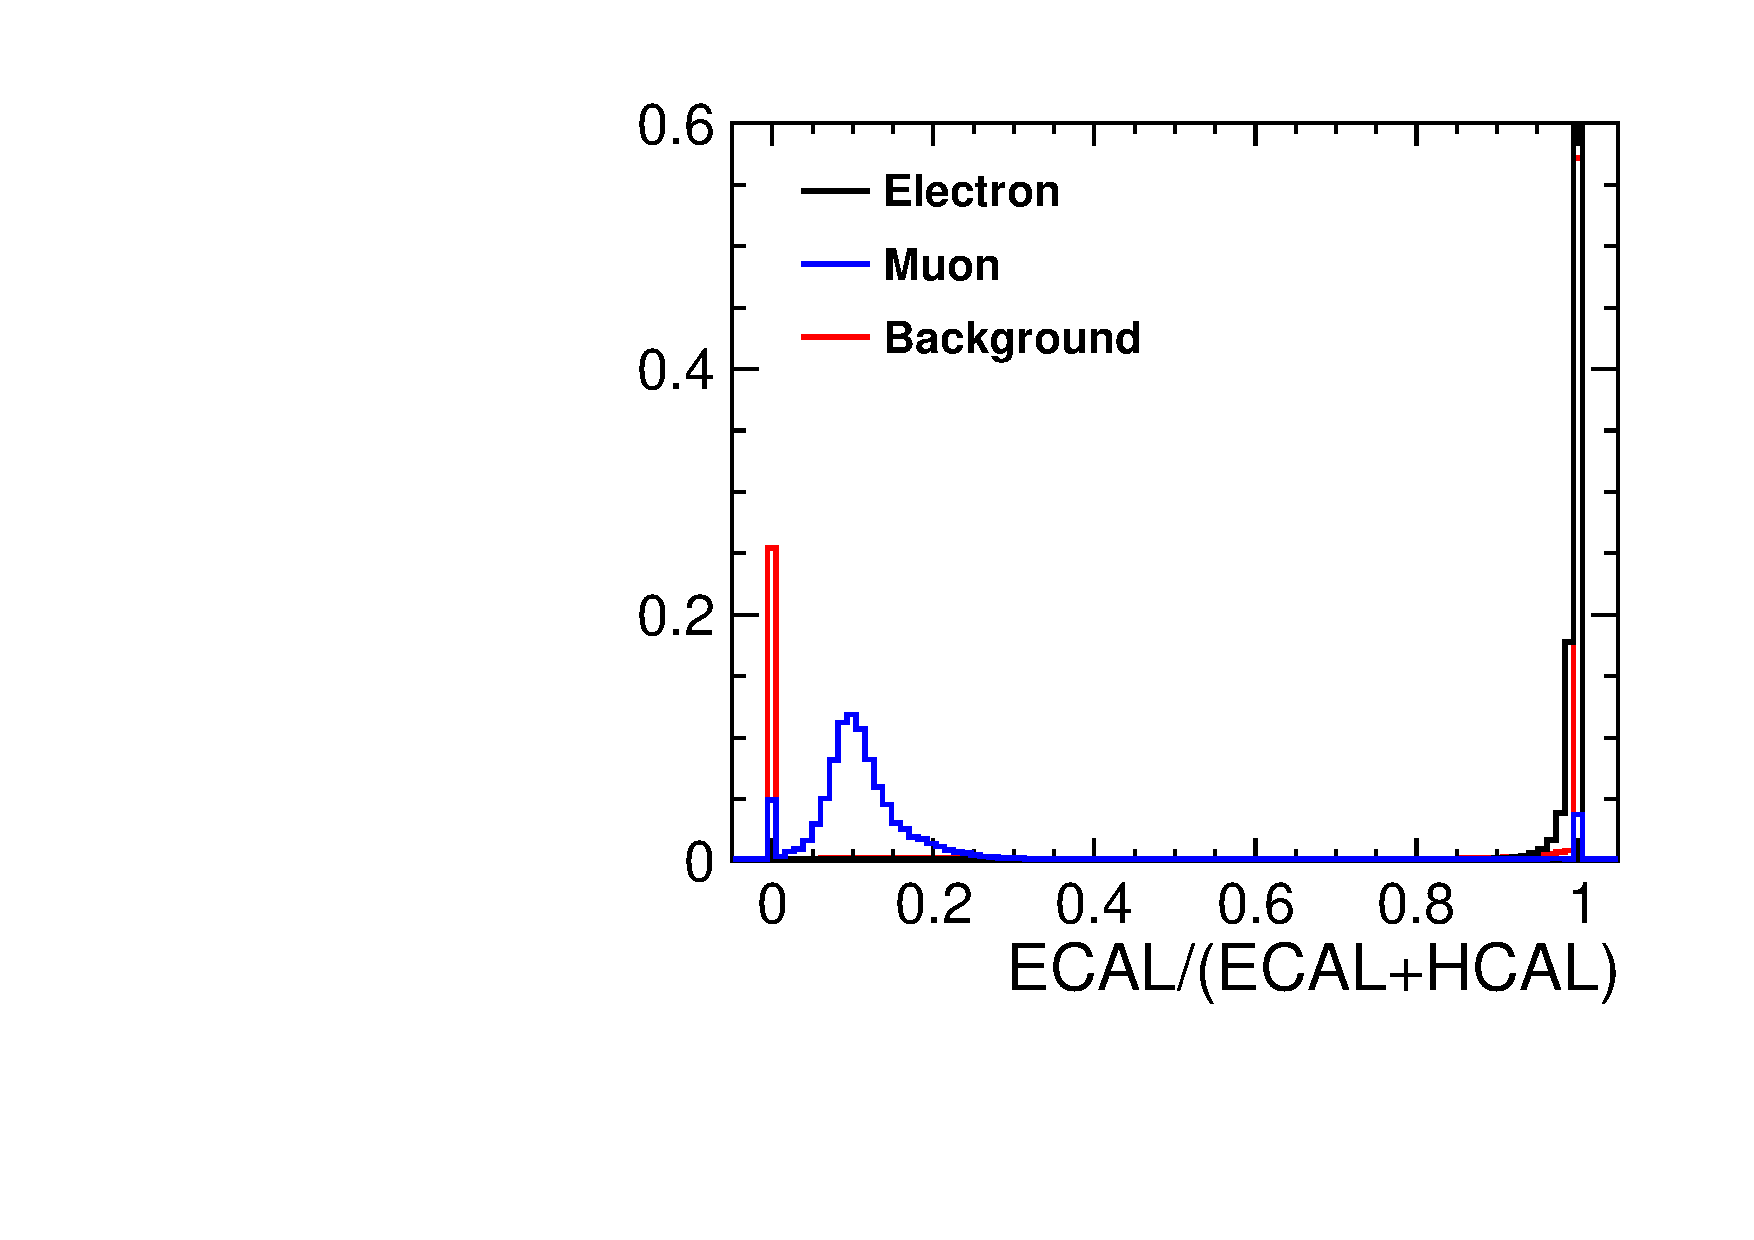
\includegraphics[width=1.0\linewidth,keepaspectratio]{HiggsAnalysis/figures/ECALByE}
    \caption{Ratio of the energy deposited in the ECAL to the total energy deposited in the calorimeters. }
  \end{subfigure}
  \caption[Parameters used for loose lepton selection]{Properties used for the loose lepton selection.  Note that in both cases, electrons and muons not produced in the initial W decay are counted as background.}
  \label{fig:lepfinding}
\end{figure}

The second method used a series of cuts to select the isolated lepton. The first stage of this was to group the particles in the event into four jets. This was done using FastJet \cite{Cacciari:2011ma} to implement the kt-algorithm using the E-scheme for recombination with an R-parameter of 0.4. We then required that the energy of the isolated lepton (electron or muon) constituted more than 35\% of the visible energy of the jet it was contained within. For electrons it was then required that at least 90\% of the total energy of the particle was deposited in the ECAL, and the ratio of energy to momentum for the particle was between 0.75 and 1.25. For muons it was required that less than 35\% of the total energy of the particle was deposited in the ECAL, and the ratio of energy to momentum should be between 0.01 and 0.60. The relevant distributions for these variables are shown in \reffig{fig:lepfinding}. This method yielded an efficiency of 91\% and a purity 74\%. Due to the lower purity of this method, leptons selected by this method are referred to as loose selected. Although this approach is not as performant as the first method, it allows more than one lepton to be selected. As a result it is useful for discriminating between signal and background processes (e.g. $e^+e^-\rightarrow ZZ\rightarrow qqll$) as requirements can be placed on the number of leptons identified by this selection.

In summary, the first method is used to select a single isolated lepton, which is then used for reconstruction, while the number of lepton candidates selected by the second method is used as a discriminating variable to distinguish between signal and background processes. 

\subsection{Jet Finding}
\label{higgsjetfinding}

\begin{figure}
  \centering
  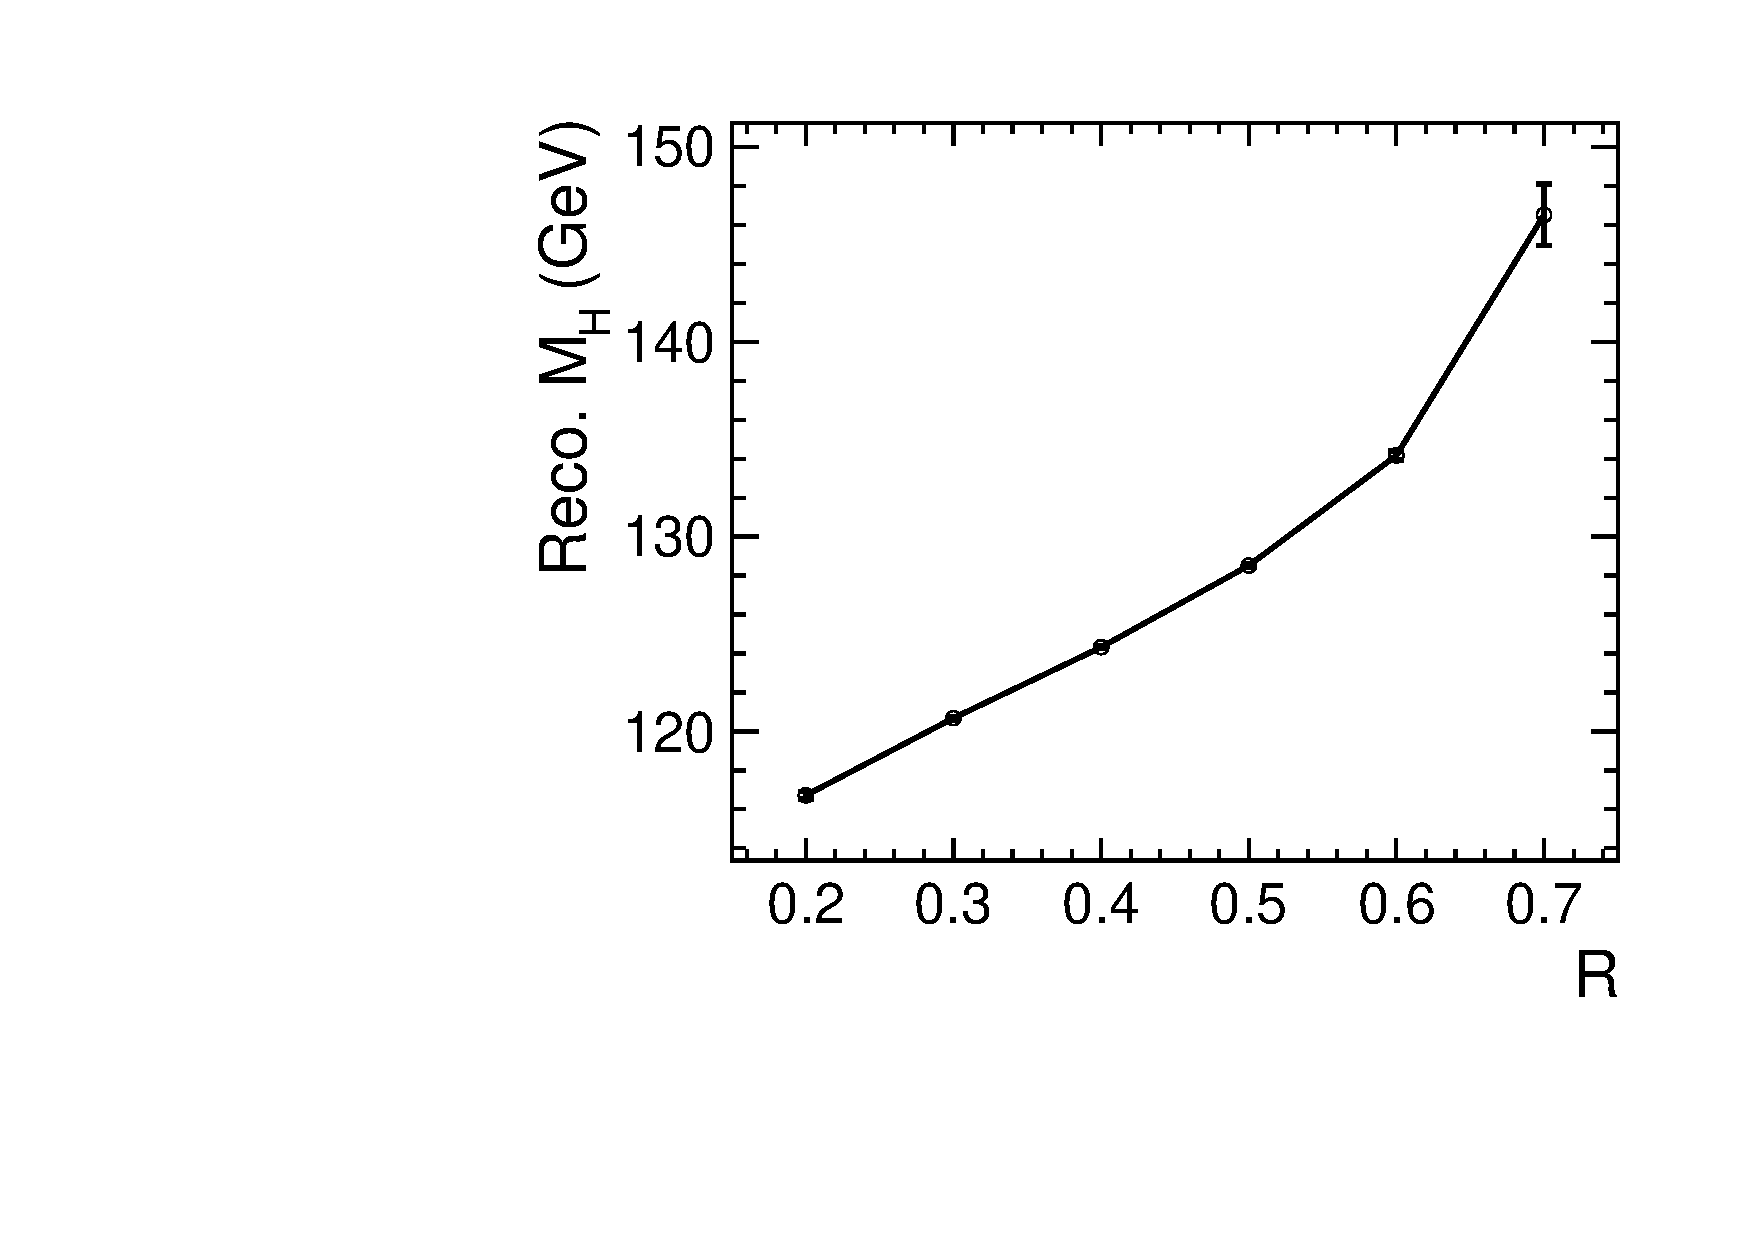
\includegraphics[width=0.7\textwidth,keepaspectratio]{HiggsAnalysis/figures/HiggsJetOptimization.pdf}
  \caption[Jet Reconstruction Optimization]{Reconstructed Higgs mass as a function of the jet radius parameter when using MC truth to add the neutrino information}
  \label{fig:jetoptimization}
\end{figure}

\begin{figure}
  \centering
  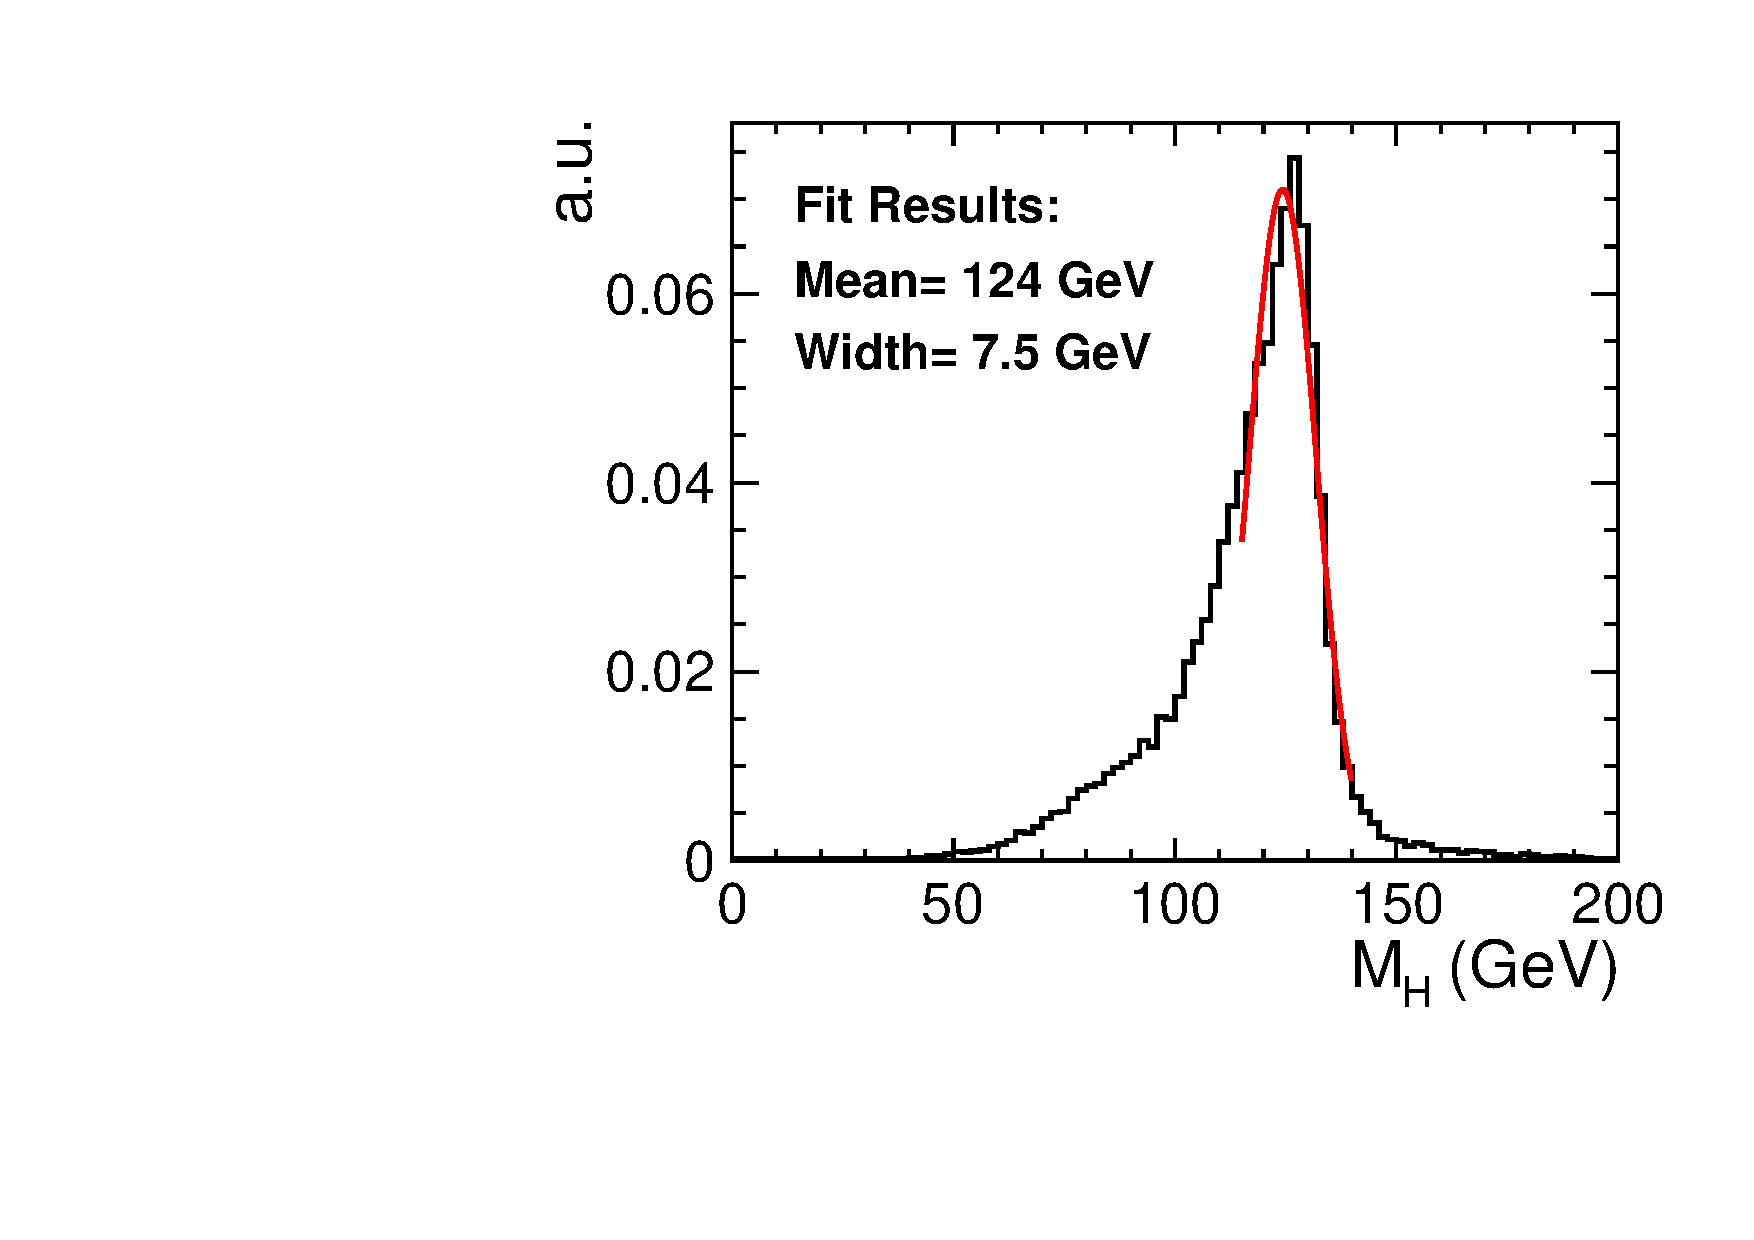
\includegraphics[width=0.7\textwidth,keepaspectratio]{HiggsAnalysis/figures/CheatHiggs04}
  \caption[Reconstructed Higgs Mass For Optimum Jet Radius]{Reconstructed Higgs mass for a jet radius of R=0.4 using MC truth information to add the neutrino information}
  \label{fig:cheatHiggsMass}
\end{figure}

\begin{figure}
  \centering
  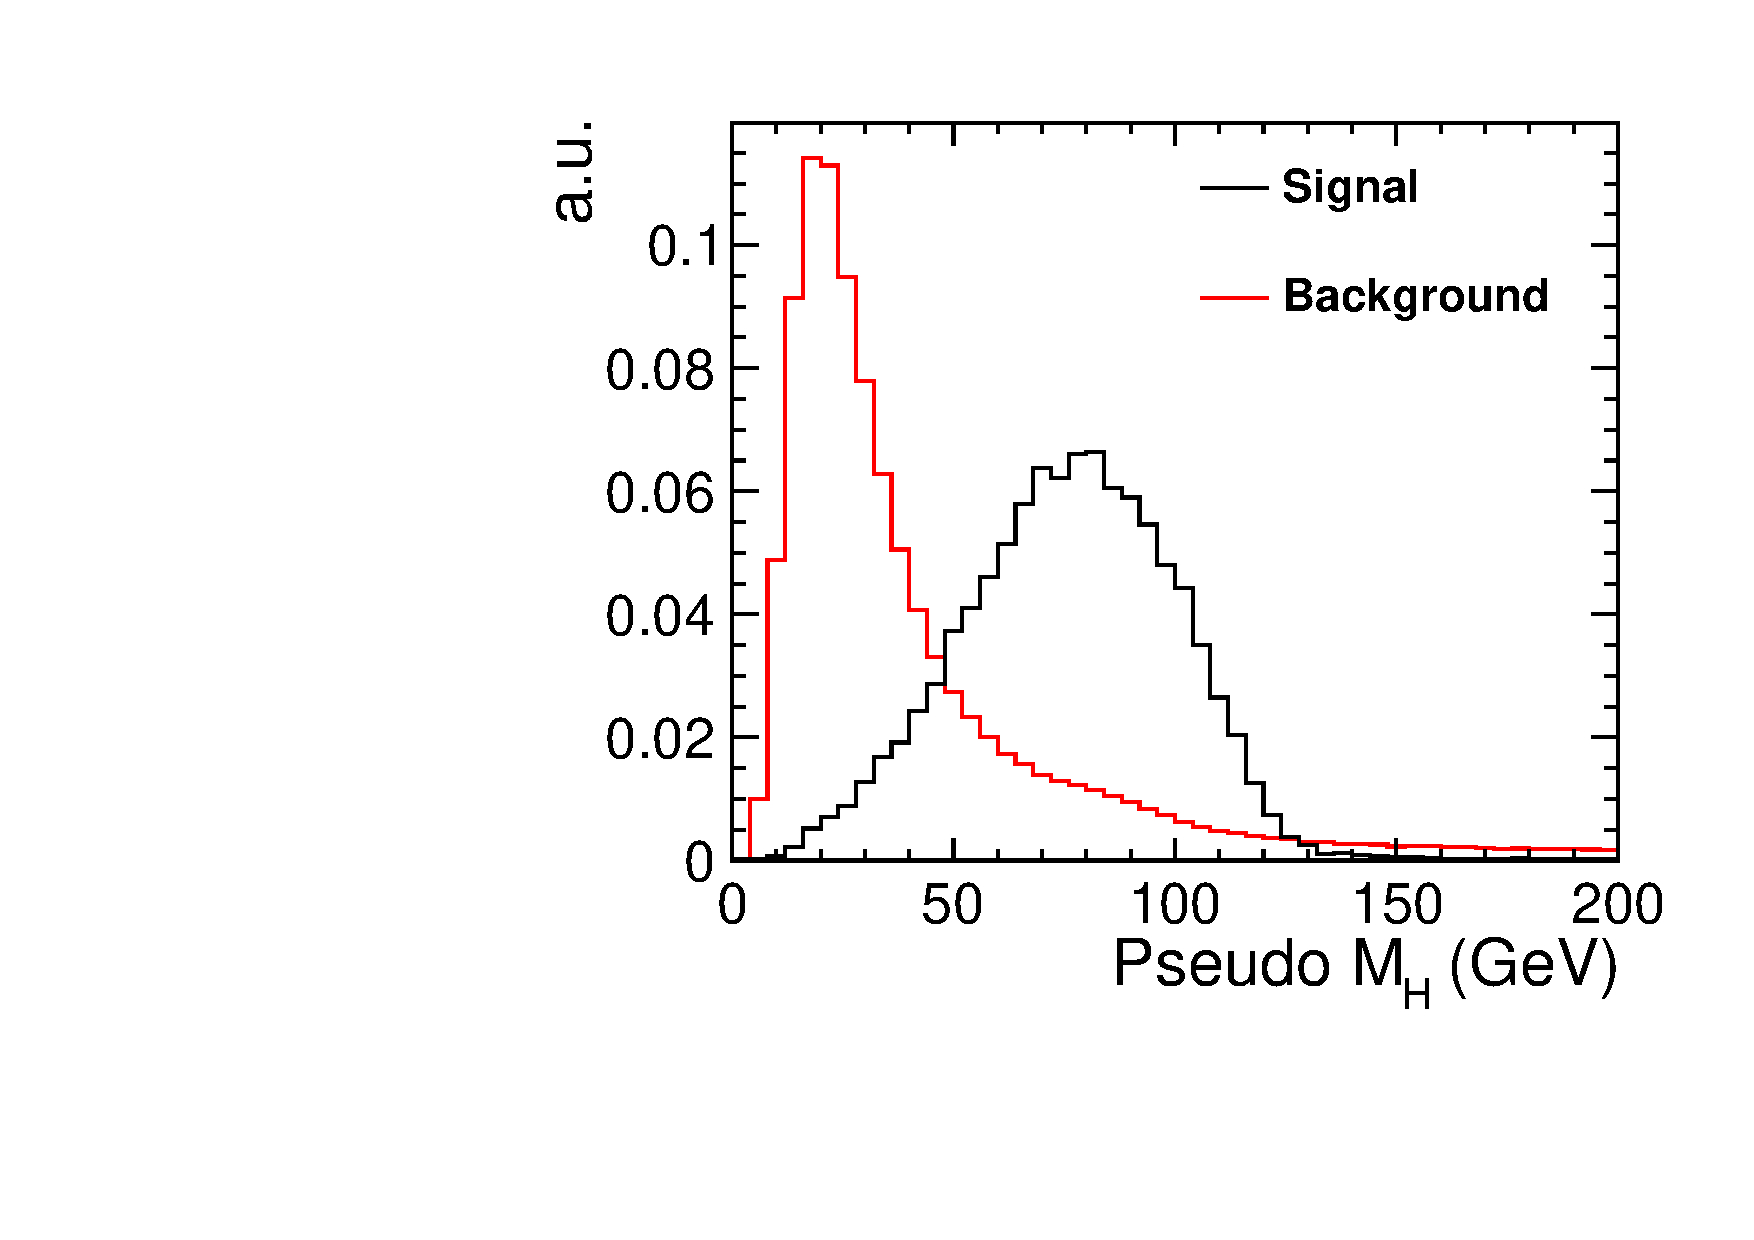
\includegraphics[width=0.7\textwidth,keepaspectratio]{HiggsAnalysis/figures/PseudoHiggs.pdf}
  \caption[Reconstructed Higgs Mass]{Reconstructed invariant mass of the lepton + quark pair system}
  \label{fig:pseudoHiggsMass}
\end{figure}


Following the lepton finding, the remaining PFOs (not including the isolated lepton) are forced into two jets to reconstruct the properties of the two quarks produced from the hadronic W decay. This was carried out using the exclusive kt algorithm as implemented in FastJet. This is a sequential jet finding algorithm and follows the following procedure:

\begin{enumerate}
\item For each particle calculate it's distance from the beam:
\begin{center}
  $d_{iB} = p_{Ti}^2$
\end{center}
\item For every pair of particles calculate the distance between them:
\begin{center}
  $d_{ij}=min(p_{ti}^2,p_{Tj}^2)\Delta R_{ij}^2/R^2$
\end{center}
where $\Delta R_{ij}^2=(y_i-y_j)^2 + (\phi_i-\phi_j)^2$, i and j label particles, p$_T$ is transverse momentum, y is rapidity, $\phi$ is azimuthal angle and R is a tuneable parameter referred to as the jet radius.
\item Find the minimum of all the $d_{ij}$ and $d_{iB}$. If this corresponds to a $d_{ij}$ then merge particles i and j by summing their four-momenta. If it corresponds to a $d_{iB}$ then declare particle i to be part of the beam and remove it.
\item Repeats steps 1)-3) until there are only the desired number of jets remaining
\end{enumerate}

The optimization of the R-parameter was performed using Monte Carlo information to determine what mass would be measured for the reconstructed Higgs for various values of R, when including the Monte Carlo truth kinematic information of the lepton neutrino in the reconstruction. The results of this optimization study are shown in \reffig{fig:jetoptimization}. An acceptably small bias in the reconstructed mass was found for an R value of 0.4, indicating successfull reconstruction of the quark pair. The resulting Higgs mass distribution is shown in \reffig{fig:cheatHiggsMass}. Note that this mass is only used for optimization of the jet reconstruction. It is never used for the event selection as it is not possible to calculate this mass without using MC truth information. For event selection, the pseudo Higgs mass corresponding to the invariant mass of the lepton and quark pair system is used instead. This is shown in \reffig{fig:pseudoHiggsMass}.



\section{Flavour Tagging}

\begin{figure}
  \centering
  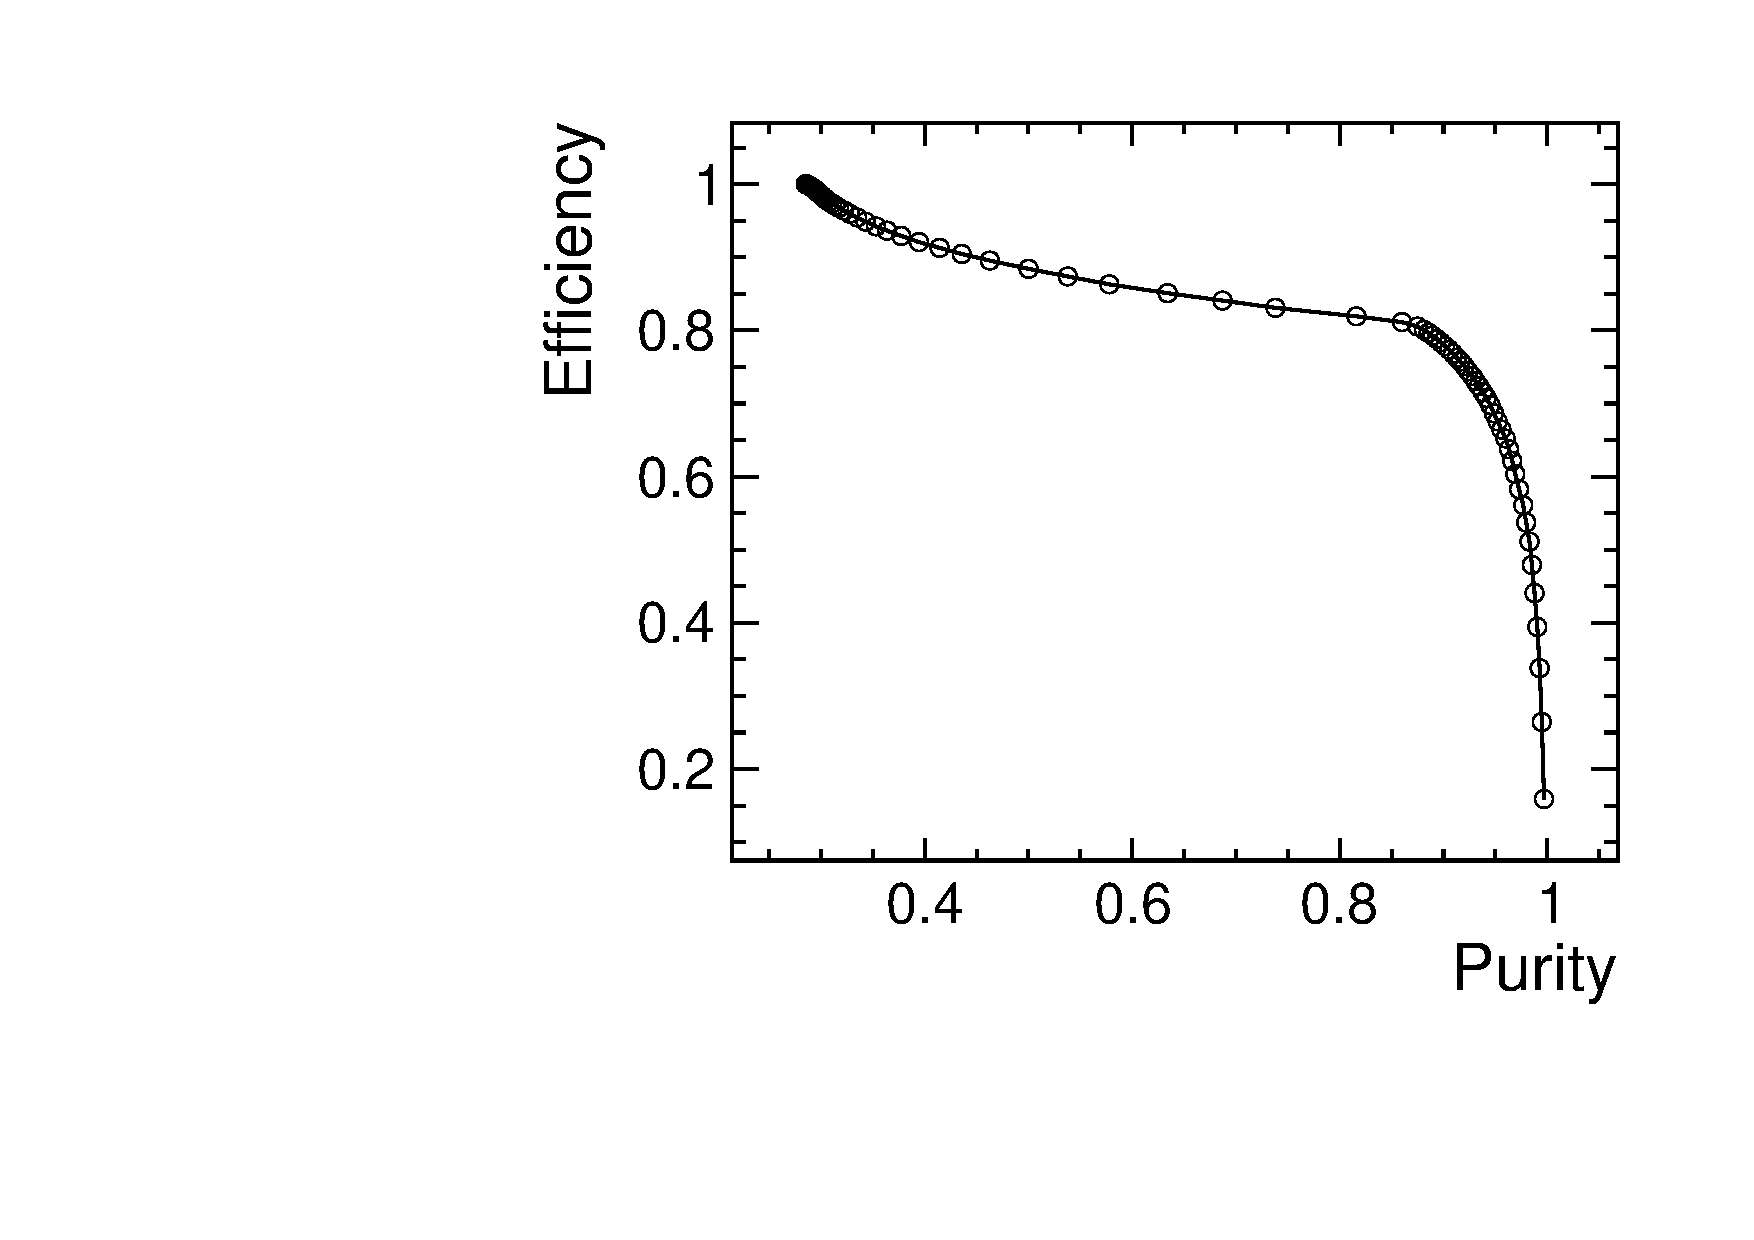
\includegraphics[width=0.78\textwidth,keepaspectratio]{HiggsAnalysis/figures/updatedpurityvsefficiency.pdf}
  \caption[B-Tagging Purity vs Efficiency]{Purity vs efficiency for identifying b-jets, obtained from a sample of Z$\rightarrow$ light, c and b quark events simulated at $\sqrt{s}=$1.4TeV.}
  \label{btag}
\end{figure}

Flavour tagging of events was performed using LCFIPlus v00-05-02 \cite{Suehara:2015ura}. Three neural nets were trained to identify u/d/s, b and c quarks respectively with 50,000 ee$\rightarrow$ Z$\nu\nu$, Z$\rightarrow$qq events used for each neural net. Application of these neural nets returned two parameters for jets within the event that quantify the probability of the jet being either a b-jet or c-jet. For this analysis, identifying b-jets is more useful for discriminating against the relevant backgrounds. Performance of the b-tagging was evaluated by applying the neural nets to a sample of 150,000 events containing an equal number of Z$\rightarrow$ light, c and b quarks. It can be seen from \reffig{btag} that a purity of 90\% can be achieved while still retaining an efficiency of 80\%.

\section{Event Selection}

Event selection was performed in two steps. The first of these is referred to as the preselection and acts to remove easily identifiable backgrounds with minimal loss of signal events by applying loose cuts. The cuts used were as follows:

\begin{enumerate}

\item Mass of the reconstructed Higgs $<$ 200 GeV
\item At least one loose selected lepton in the event
\item Missing energy of the event must lie in the range 800--1350 GeV
\item Energy of the hadronically decaying W $<$ 600 GeV

\end{enumerate}


\begin{figure}
  \centering
  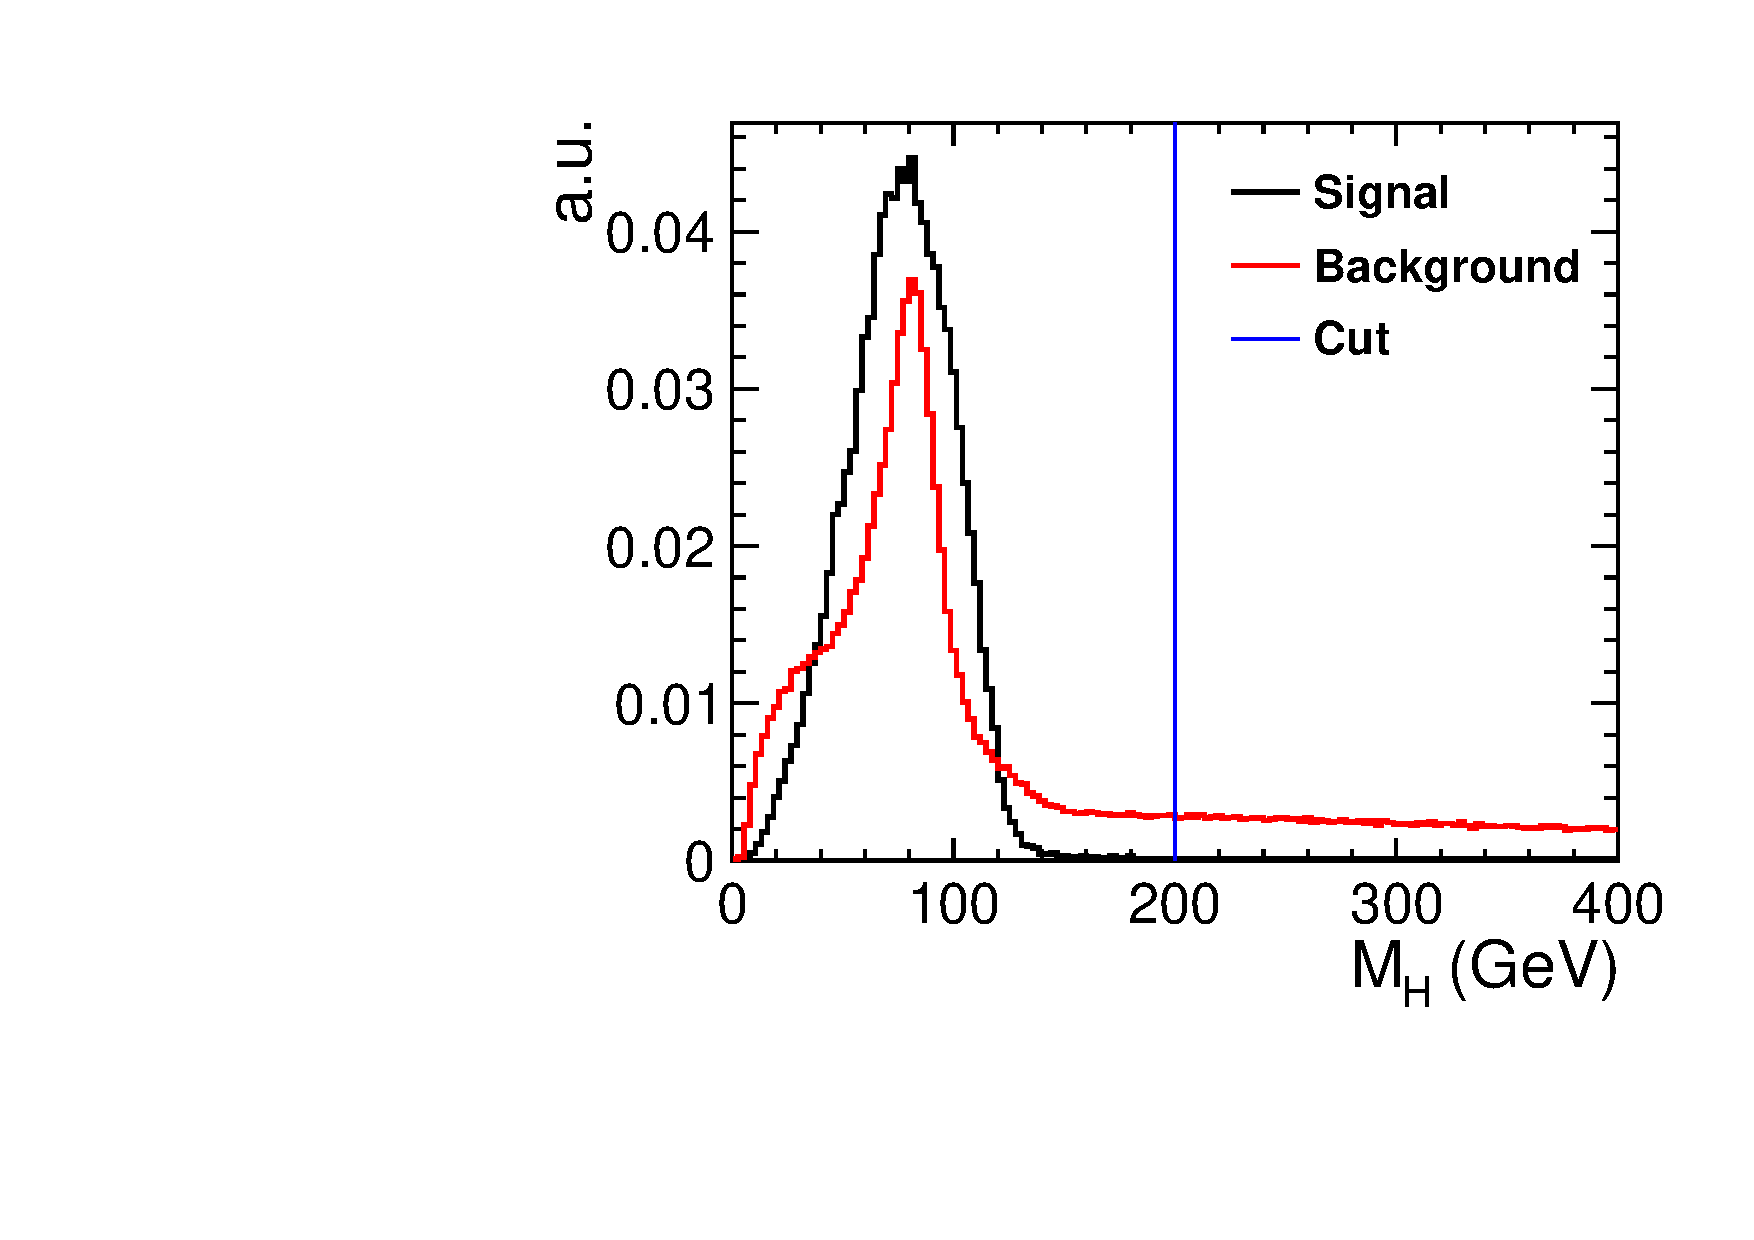
\includegraphics[width=0.78\textwidth,keepaspectratio]{HiggsAnalysis/figures/PseudoHiggs_PreSelection}
  \caption[Reconstructed Higgs mass for signal and background events]{Mass of the reconstructed Higgs for the signal process and dominant backgrounds ($ee\rightarrow H\nu\nu$ (non-signal) and $ee\rightarrow qql\nu$).}
  \label{fig:HMassPreSel}
\end{figure}

\begin{figure}
  \centering
    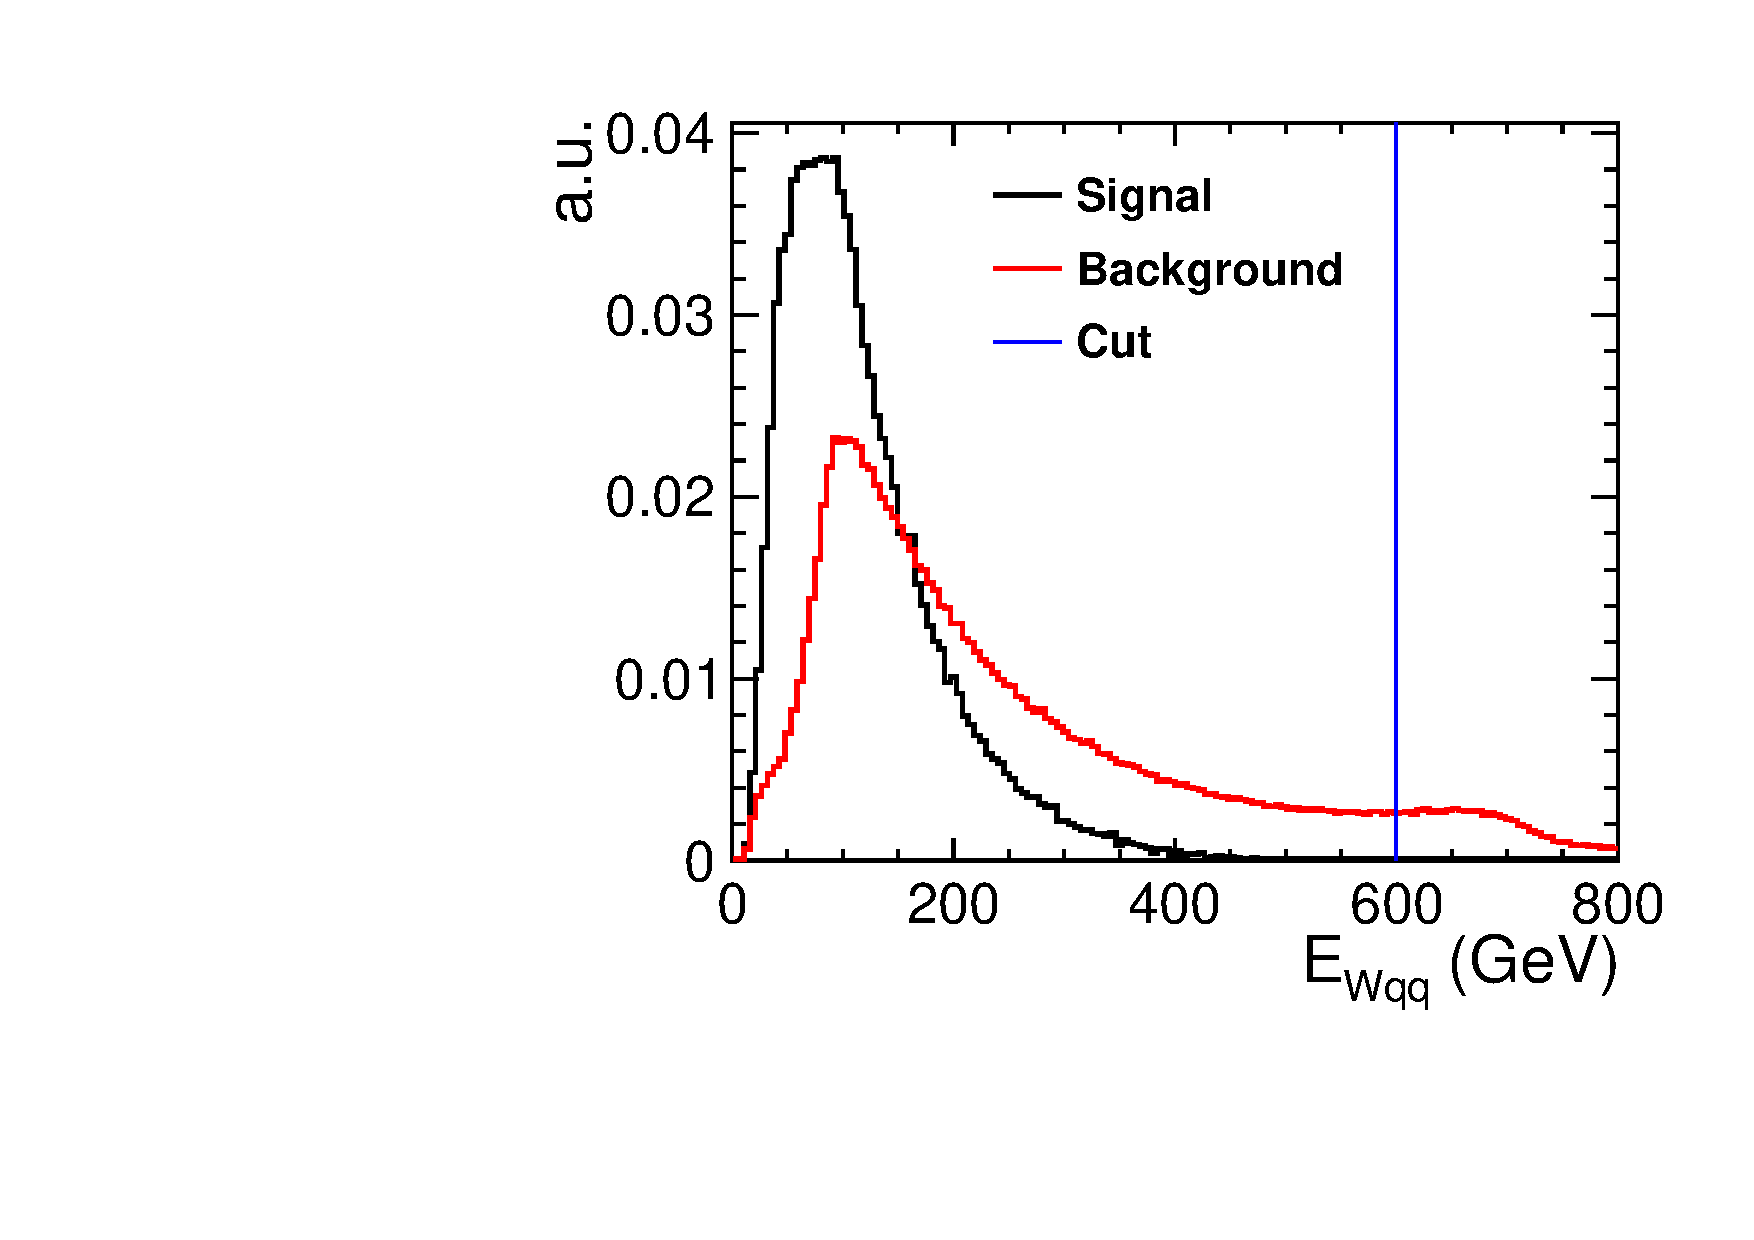
\includegraphics[width=0.78\linewidth,keepaspectratio]{HiggsAnalysis/figures/EWqq_PreSelection}
    \caption[Energy of the hadronically decaying W Boson for signal and background events]{Energy of the hadronically decaying W Boson for the signal process and dominant backgrounds ($ee\rightarrow H\nu\nu$ (non-signal) and $ee\rightarrow qql\nu$).}
  \label{fig:WPreSel}
\end{figure}

\begin{figure}
  \centering
  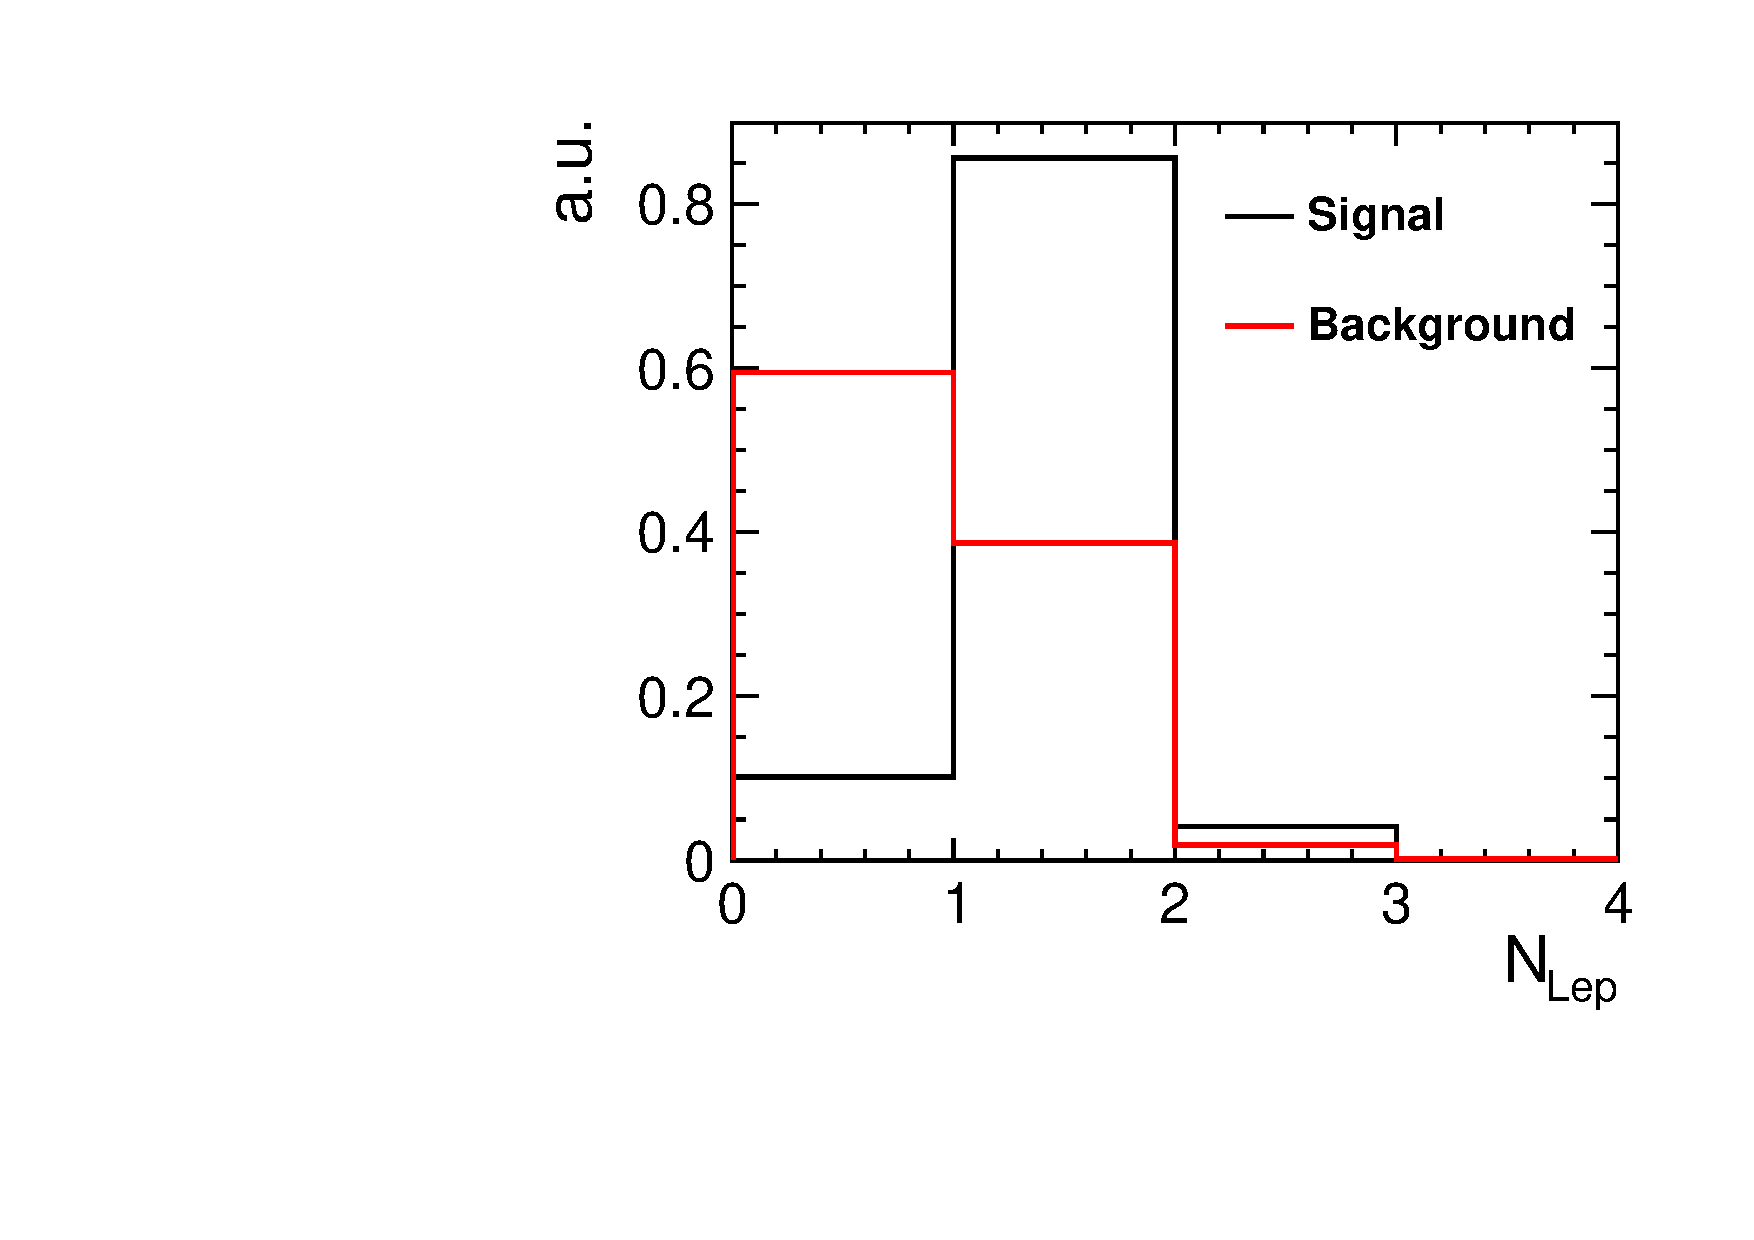
\includegraphics[width=0.78\textwidth,keepaspectratio]{HiggsAnalysis/figures/nLep_PreSelection}
  \caption[Number of reconstructed loose selected lepton for signal and background events]{Number of loose selected leptons for the signal process and dominant backgrounds ($ee\rightarrow H\nu\nu$ (non-signal) and $ee\rightarrow qql\nu$)}
  \label{fig:nLepPreSel}
\end{figure}

\begin{figure}
  \centering
  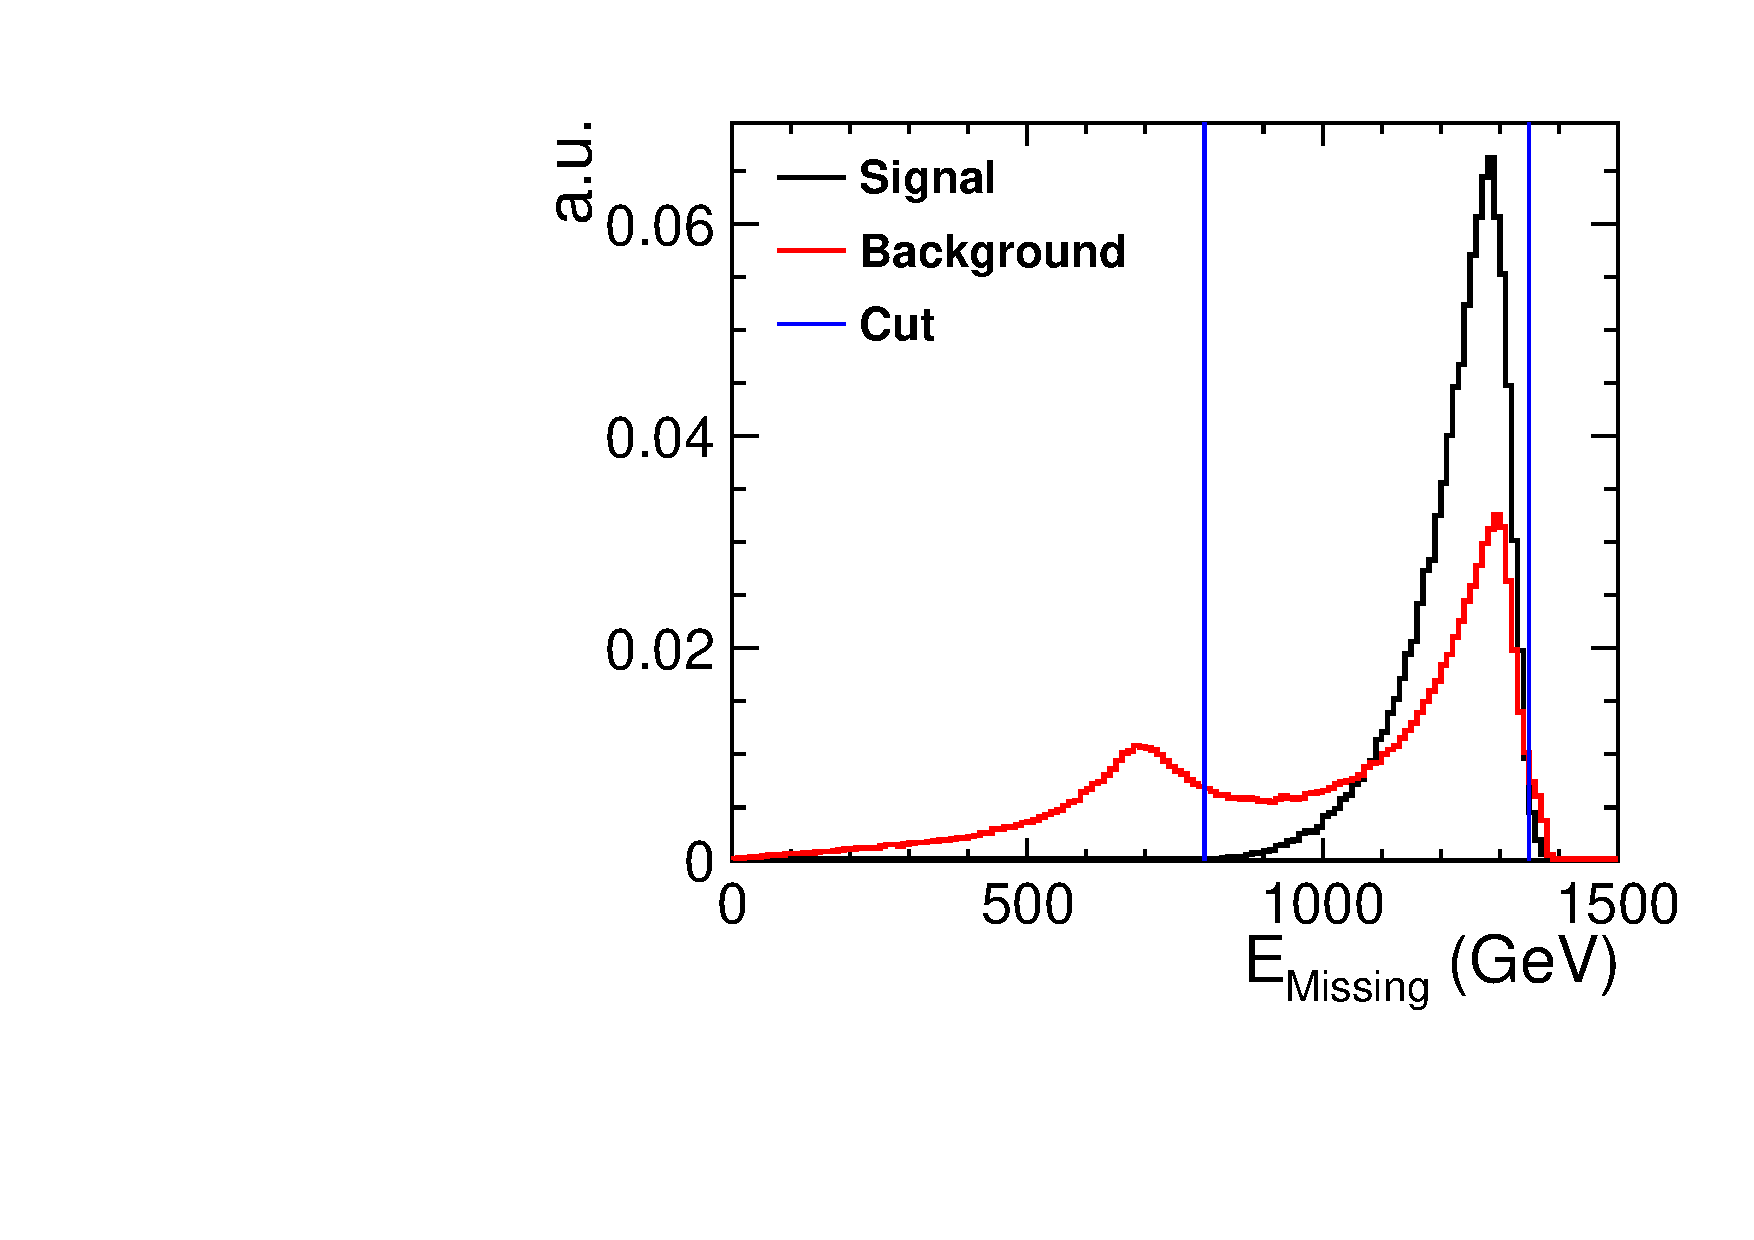
\includegraphics[width=0.78\textwidth,keepaspectratio]{HiggsAnalysis/figures/EMissing_PreSelection}
  \caption[Missing energy of signal and background events]{Missing energy for the signal process and dominant backgrounds ($ee\rightarrow H\nu\nu$ (non-signal) and $ee\rightarrow qql\nu$).}
  \label{fig:EMissPreSel}
\end{figure}

\begin{figure}
  \centering
  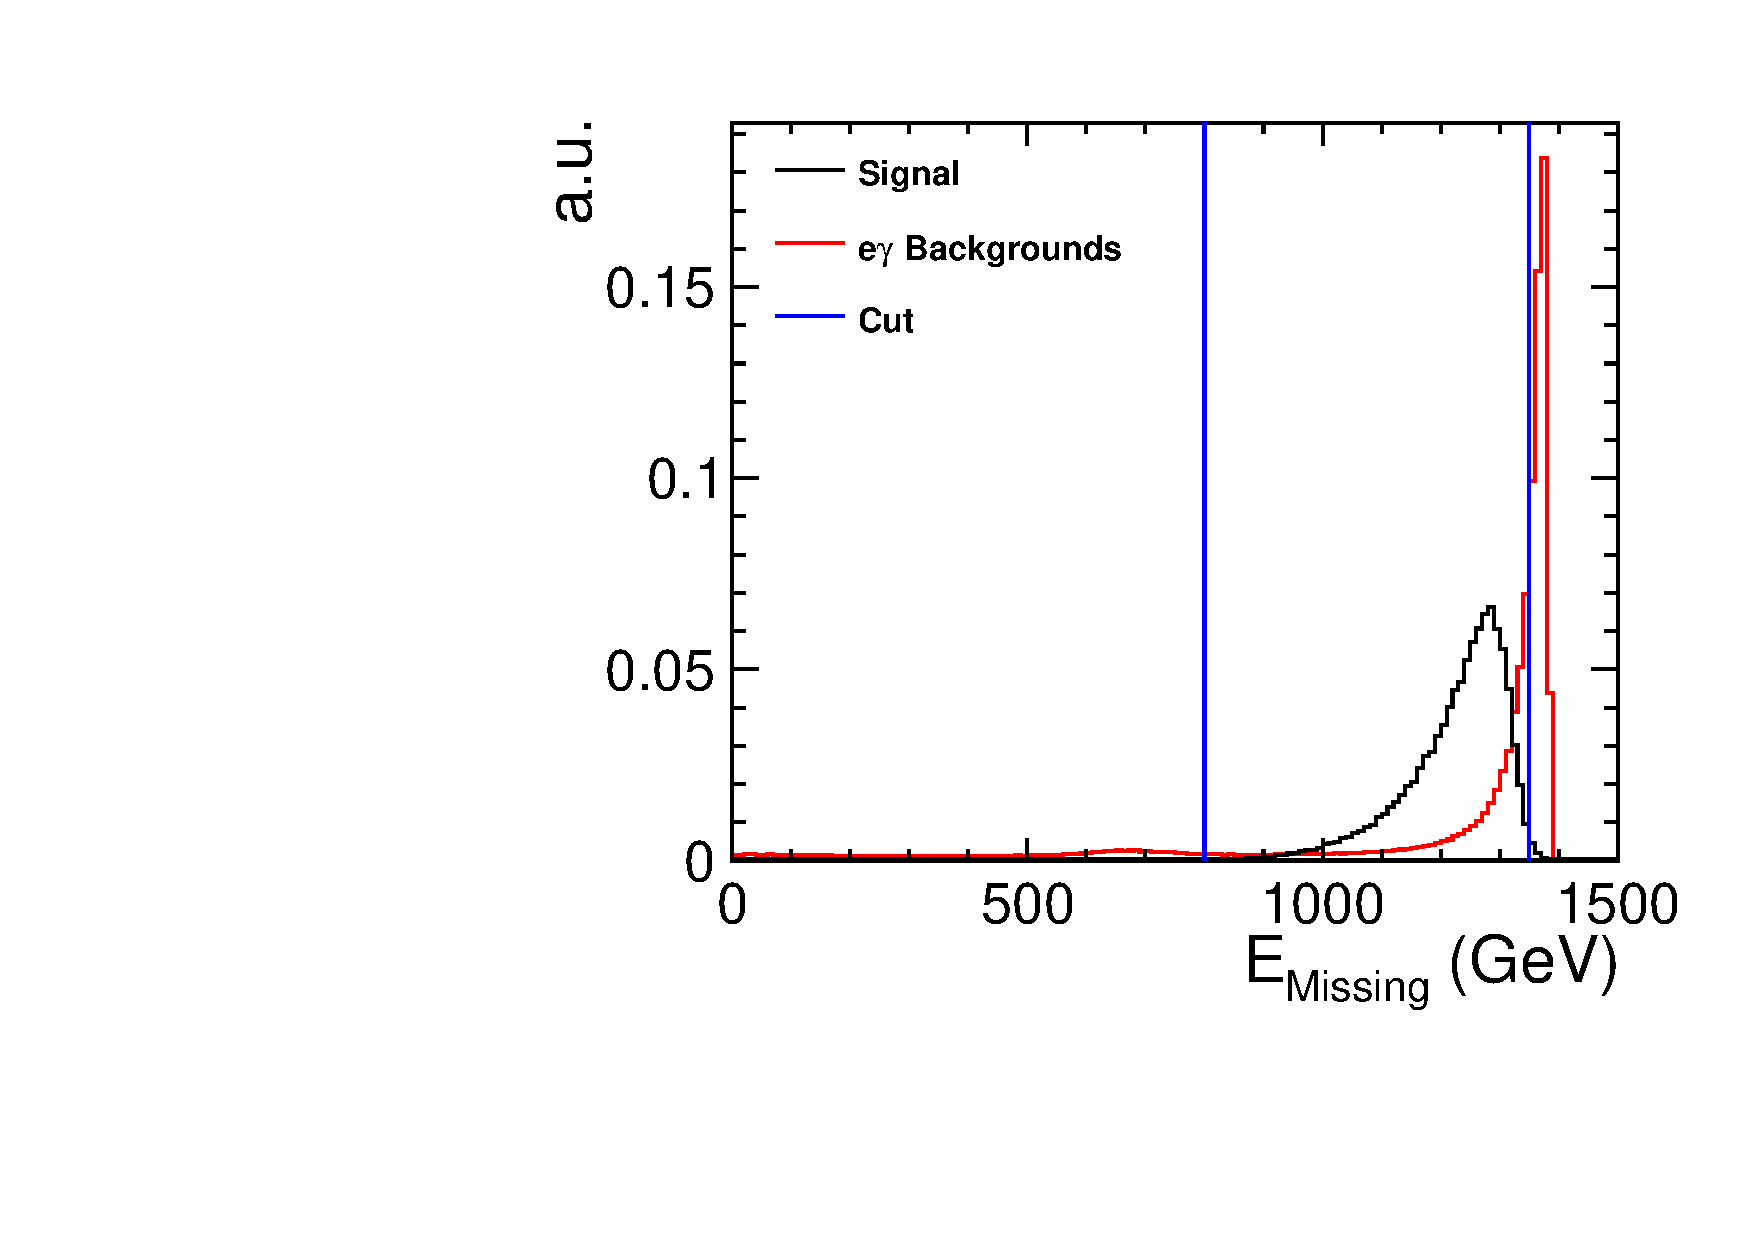
\includegraphics[width=0.78\textwidth,keepaspectratio]{HiggsAnalysis/figures/EMissing_PreSelection_alt}
  \caption[Missing energy of signal and e$\gamma$ events]{Missing energy for the signal process and e$\gamma$ backgrounds.}
  \label{fig:EMissPreSelAlt}
\end{figure}

\begin{figure}
  \centering
  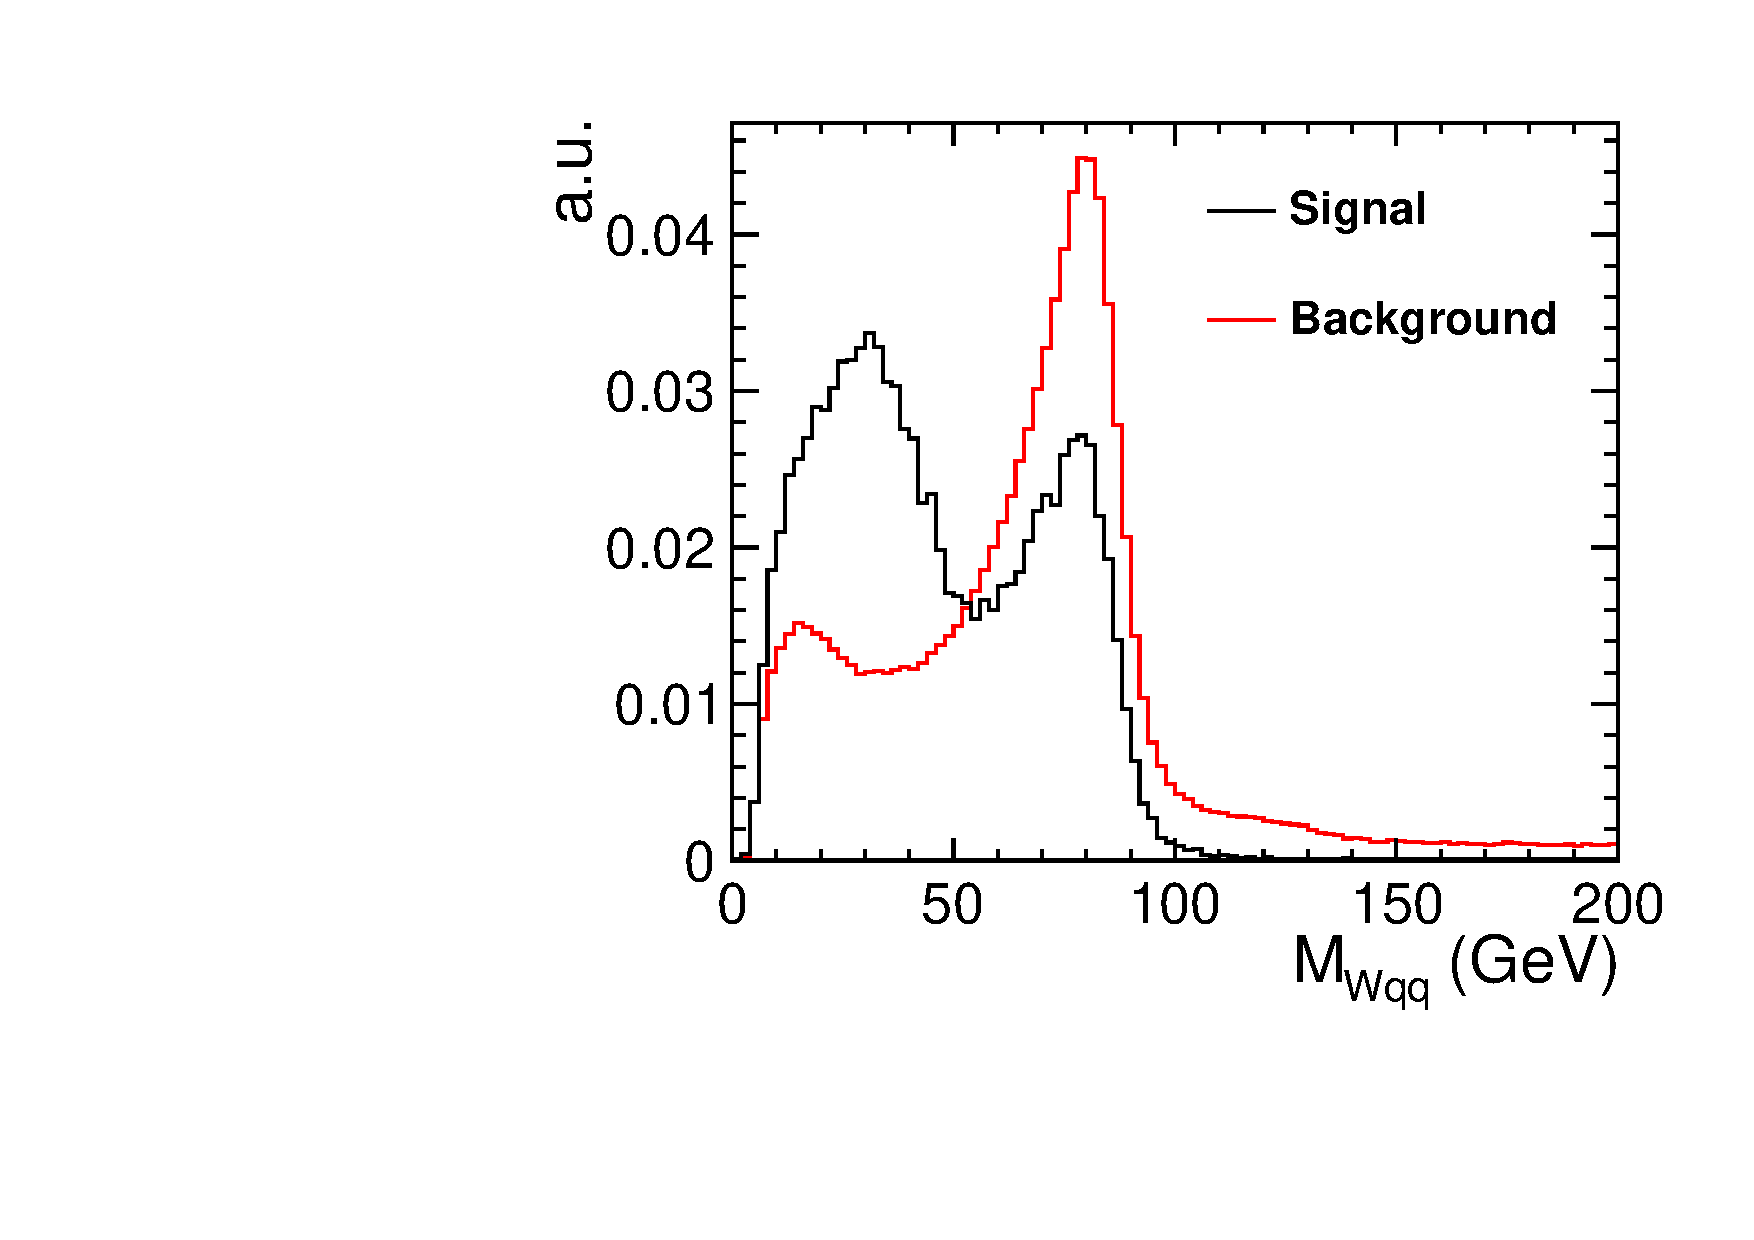
\includegraphics[width=0.78\textwidth,keepaspectratio]{HiggsAnalysis/figures/MWqq_PreSelection}
  \caption[Reconstructed W mass for signal and background events]{Reconstructed mass for the signal process and dominant backgrounds ($ee\rightarrow H\nu\nu$ (non-signal) and $ee\rightarrow qql\nu$).}
  \label{fig:WMass}
\end{figure}


With the exception of the upper limit placed on the missing energy, these cuts were optimised for the removal of the two dominant background processes ($ee\rightarrow H\nu\nu$ (non-signal) and $ee\rightarrow qql\nu$.) The upper limit on missing energy is instead designed to remove $e\gamma$ events which are typically collinear to the beam axis and so eave minimal energy in the detector. This cut alone removes approximately half of all $e\gamma$ events. The distribution of the variables associated with these cuts before the preselection is applied are shown for the signal and dominant backgrounds($ee\rightarrow H\nu\nu$ (non-signal) and $ee\rightarrow qql\nu$)in \reffig{fig:HMassPreSel}-\ref{fig:EMissPreSelAlt} and the resulting efficiencies for the signal and background processes after the preselection is applied are shown in \reftab{fig:preseleff}. Along with the cut on the mass of the Higgs, one might naively expect a similar cut to be placed upon the mass of the reconstructed W. However, due to the relative masses of the Higgs and W the W's produced in the Higgs decay cannot always be on shell. In practice one finds that the kinematically favoured solution is that one W is produced on shell while the second is produced with a mass of $\sim$45 GeV. As a result, as can be seen in \reffig{fig:WMass}, it is challenging to separate background events from signal events in which the hadronically decaying W is produced off shell.

\begin{figure}
  \centering
  \begin{tabular}{l r r }
   \toprule
    Process & Cross Section(fb) & Preselection Efficiency (\%)     \\
    \midrule
    Signal             & 17.3    &   89.3 \\ 
    \midrule
    ee$\rightarrow$ H(WW$^*\rightarrow$qqqq)$\nu\nu$  & 27.4    &  4.12  \\
    \midrule
    ee$\rightarrow$ H($\rightarrow$ Other)$\nu\nu$ & 199.4 & 26.4  \\
    \midrule
    ee$\rightarrow$qq               & 4009.5    &  7.21 \\ 
    \midrule
    ee$\rightarrow$qqqq               & 1328.1    &  2.09  \\ 
    \midrule
    e$\gamma$$\rightarrow$eqq ($\gamma$ from EPA)                 & 32308    & 7.32   \\ 
    \midrule
    $\gamma$e$\rightarrow$eqq ($\gamma$ from BS)               &  56043   &  8.02 \\ 
    \midrule
    ee$\rightarrow$qq$\nu\nu$               & 787.7    & 9.18  \\ 
    \midrule
    ee$\rightarrow$qqll               & 2725.8    &   13.6 \\ 
    \midrule
    ee$\rightarrow$qql$\nu$              & 4309.7    &  7.90  \\ 
    \bottomrule
  \end{tabular}
  \caption[Preselection efficiencies]{Preselection efficiencies}
  \label{fig:preseleff}
\end{figure}



\subsection{Boosted Decision Trees}

\begin{figure}
  \centering
  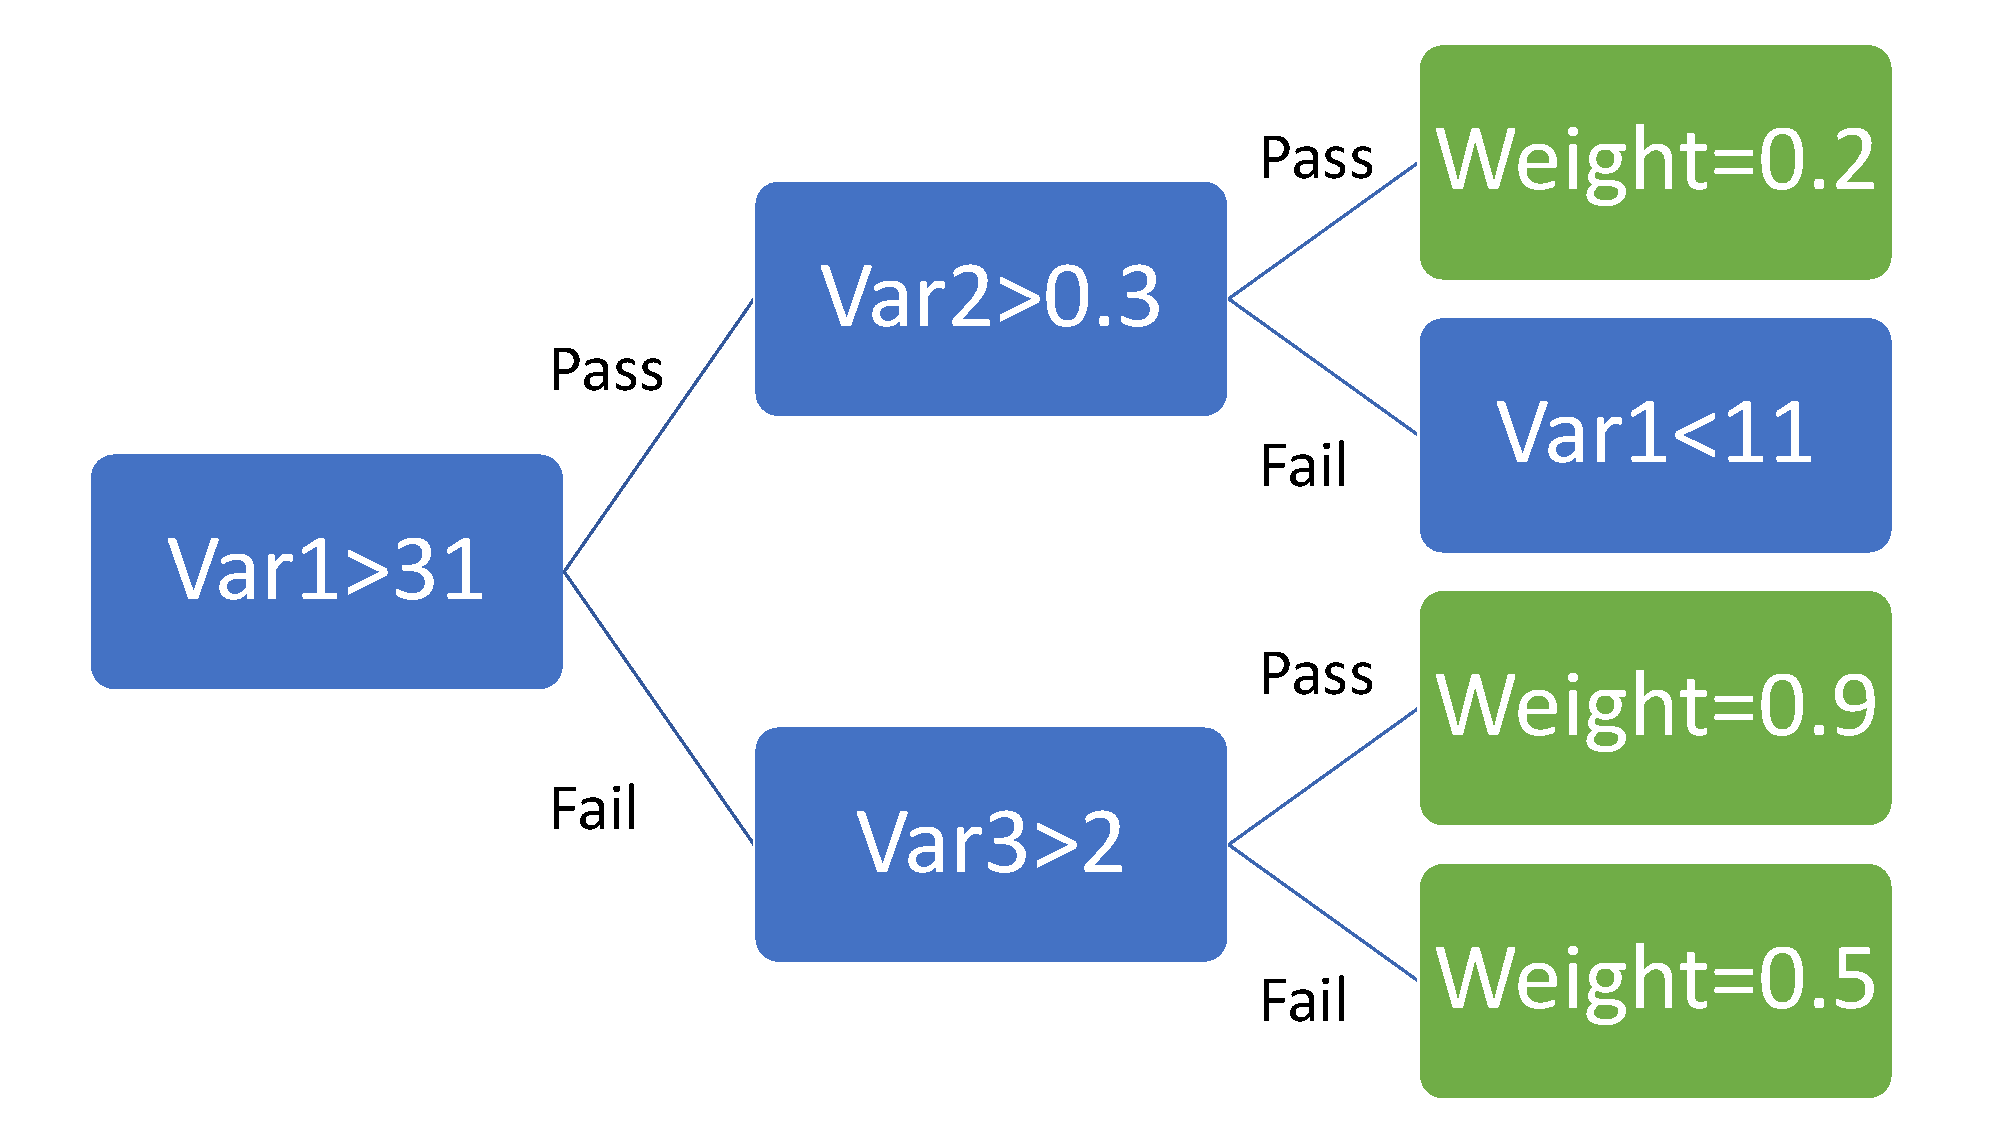
\includegraphics[width=0.78\textwidth,keepaspectratio]{HiggsAnalysis/figures/decisiontree}
  \caption[Example of a decision tree]{Example of a decision tree. Blue represents nodes while green represents leaves}
  \label{fig:decisiontree}
\end{figure}

Following the preselection, the main event selection is then performed using a multivariate approach that takes into account correlations between variables to maximise the information available for background discrimination. A \ac{BDT}, implemented in ROOT TMVA \cite{2007physics...3039H} was used for performing this stage of the selection. A detailed description of how a BDT works is given in \cite{Coadou:2013lca}. Fundamentally a decision tree can be represented as a logic flow diagram that assigns a weight to an event based on a series of cuts e.g. see \reffig{fig:decisiontree}. Each level of the flow chart is made up of nodes and leafs. A node represents a cut on a particular variable where the specific choice of cut is chosen to be that which provides the greatest separation between signal and background. A leaf on the other hand represents an end point at which a weight (typically chosen to be the purity of events reaching that point) is assigned to the event. The choice of whether to create a leaf or node after each branching is decided by a stopping criteria. Typically this criteria represents producing a sufficienctly high or low purity of events that the node can be assigned to contain almost entirely signal or background. Typically not all events will have signal like properties for every variable used. As a result it is normally necessary to produce multiple trees (creatively referred to as a forest) using different combinations of variables for each of the nodes. The sum of weights from all the trees used then forms a final discriminating variable for distinguising between signal and background events. Boosting is then a way of maximising the performance of the decision trees. The simplest form of boosting is train a set of trees, T$_1$, using a sample of N events. A second set of trees, T$_2$, are then trained using a further N events, half of which were misclassified by T$_1$. A third set of trees, T$_3$,  can then be formed by training on events in which T$_1$ and T$_2$ disagree on the classification. The overall classification is then decided by a democratic vote from T$_1$, T$_2$ and T$_3$. This method yields an improvement in the performance by focusing the training on events that are the hardest to discriminate. The method can be extended to an aritrary number of levels T$_N$ where the final \ac{BDT} score is then a weighted sum of the scores from the N trees. By implementing the preselection cuts before training the \ac{BDT} the overall background rejection is found to be further improved as again, the \ac{BDT} is able to focus only on those events that are hardest to discriminate. Within TMVA, the default parameters for the training are to use 850 trees per forest with each tree having a maximum depth of three nodes. This provides a balance between the computational time required to train the classifier and the performance it can achieve however it is possible an improved performance might be achieved by increasing the number of trees per forest or the depth of each tree. 

The \ac{BDT} in this analysis used 7$\times$10$^4$ signal events and 4$\times$10$^6$ background events, split evenly between training and testing samples. A collection of 19 variables is used for the training: masses of the reconstructed Higgs and W bosons; energy of the W boson; total missing energy and transverse momentum; number of loose selected isolated leptons; PID of the isolated lepton; transverse momentum of lepton; angle of lepton and W boson relative to the beam axis; magnitude of minor thrust value; number of particle flow objects (PFOs) in the two jets; average angle of the two jets relative to the beam axis; kt jet resolution parameter y$_{12}$; number of tightly selected PFOs in the event; angular separation of the isolated lepton and W boson;  minimum angular separation and transverse momentum of the lepton relative to either jet, and the combined b-tag value for both jets. The signal and background distributions for every input variable after application of these cuts can be seen in Appendix A, and the resulting BDT classifier output can be seen in \reffig{bdt}.  

\begin{figure}
  \centering
  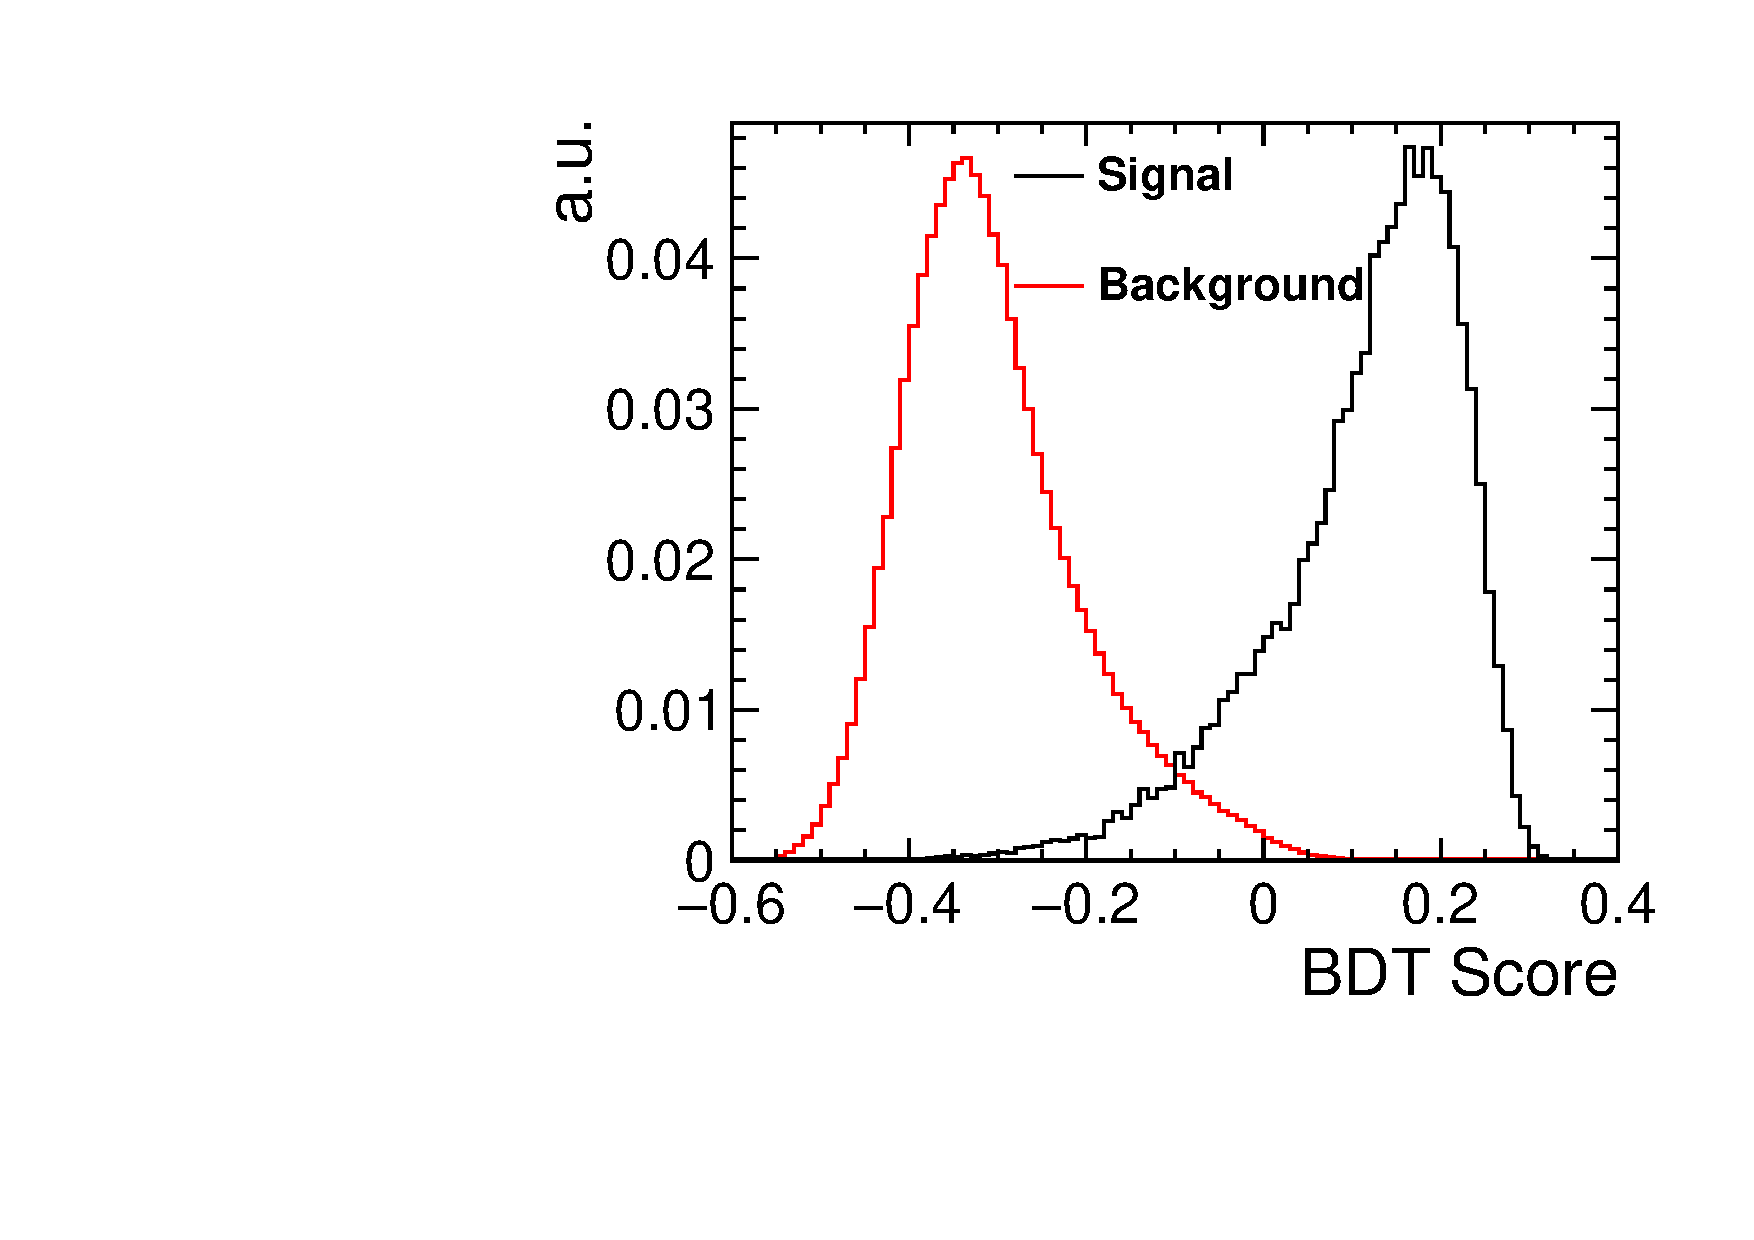
\includegraphics[width=0.78\textwidth,keepaspectratio]{HiggsAnalysis/figures/bdtscore}
  \caption[Classifier BDT response]{BDT response for signal and background events after TMVA classification. Each distribution is normalised to unity.}
  \label{bdt}
\end{figure}

\reffig{bdt} shows that there is a high degree of separation achieved between signal and background events.
The choice of cut on the BDT score was initially chosen to maximise the signal significance ($S/\sqrt{S+B}$) as this corresponds to the lowest statistical uncertainty on $\sigma\times$BR. Doing this it was found that a maximum significanc of 77 was possible by applying a cut on the BDT score of 0.15, corresponding to a statistical uncertainty of 1.30\% on $\sigma\times$BR. However, after later considerations of the the relevant systematic uncertainties associated with the measurement (see \refsec{higgsSystematics}), it was found that the overall uncertainty could be reduced by imposing a harsher cut of 0.17 on the BDT score resulting in a statistical uncertainty of 1.34\% on $\sigma\times$BR assuming an integrated luminosity of 1.5 ab$^{-1}$.

This value is similar to that observed for the WW$\rightarrow$qqqq final state, 1.5\%, as expected. By neglecting the case where the isolated lepton it a $\tau$, we have reduced our statistical sample to two thirds that of the hadronic channel which inherently limits the precision that can be acheived. However, due to the lack of an easily identifiable isolated lepton and the combinatorics associated with assigning the four jets to the two W's, the signal in the qqqq channel is more challenging to distinguish from background events.

Looking in detail at the backgrounds after our selection, we can see that many of the backgrounds have been almost completely removed leaving only ee$\rightarrow$ H($\rightarrow$ other)$\nu\nu$ and ee$\rightarrow$qql$\nu$ as the dominant backgrounds. This is to be expected as these events most closely mimic our signal, which is mainly distinguished by its large missing energy. In the case of H$\rightarrow$other events it was determined that 26\% of the remaining events came from H$\rightarrow\tau^+\tau^-$ processes with a further 25\% from H$\rightarrow$WW* processes with one or more of the Ws decaying to a $\tau$. As such, attempts were made to veto $\tau$ events by rejecting events in which one or more hadronically decaying $\tau$ was explicitly identified using the default ILCSoft Tau Finder \cite{TauFinder} package. However, the number of fake $\tau$'s identified in the signal channel was determined to be too high to veto the $\tau$ events without significantly increasing the overall statisitcal uncertainty on $\sigma \times$BR and so $\tau$ identification is not used in the final selection. It is anticipated that in a scenario where \ac{CLIC} is commisioned, an updated version of the tau finder package would be developed. One obvious improvement that could be made to the finder would be to include particle ID information as determined from Pandora for identifying taus. With a sufficiently performant tau finder, up to 50\% of the current backgrounds could potentially be removed. 

The efficiency for selecting WW$^*\rightarrow$qqqq events in the WW$^*\rightarrow$qql$\nu$ channel has been calculated to be 0.2\%. The converse efficiency for selecting WW$^*\rightarrow$qql$\nu$ events in the WW$^*\rightarrow$qqqq channel is 1.0\% which should be sufficiently low that a straightforward combination of the uncertainties determined by both channels can be made. The resulting combined statistical uncertainty on $ee\rightarrow H\nu\nu, H\rightarrow WW^*$ is expected to be $\sim$1.0\%.

\begin{figure}
  \centering
  \begin{tabular}{l c c c c}
   \toprule
    Process & Cross Section & Pre-selection & BDT Cut  & Events After BDT     \\
    & (fb) & Eff. & Eff. &      \\
    \midrule
    \midrule
    \bf{ee$\rightarrow$H$\nu\nu$;}            & \bf{17.3}    &  \bf{8.93E-01}  & \bf{3.63E-01} & \bf{9409}    \\
    \bf{H$\rightarrow$WW$^*\rightarrow$qql$\nu$} & & & & \\
    \midrule
    \midrule
    ee$\rightarrow$H$\nu\nu$;  & 27.4    & 4.12E-02 & 2.03E-03 & 84  \\
    H$\rightarrow$WW$^*\rightarrow$qqqq & & & & \\
    ee$\rightarrow$H$\nu\nu$; & 199.4 & 2.64E-01 & 6.93E-03 & 2072 \\
    H$\rightarrow$Other & & & & \\
    \midrule
    \midrule
    ee$\rightarrow$qq               & 4009.5    & 7.21E-02 &  1.72E-05 & 103  \\ 
    ee$\rightarrow$qqqq               & 1328.1    &  2.09E-02 & 3.37E-05 & 67   \\ 
    e$\gamma$$\rightarrow$eqq ($\gamma$ from EPA)                 & 32308    & 7.32E-02  & 1.26E-05 & 612  \\ 
    $\gamma$e$\rightarrow$eqq ($\gamma$ from BS)               &  56043   & 8.02E-02 & 4.54E-06 & 382  \\ 
    ee$\rightarrow$qq$\nu\nu$               & 787.7    & 9.18E-02 & 3.41E-04 & 403   \\ 
    ee$\rightarrow$qqll               & 2725.8    & 1.36E-01  & <1.93E-05 & 79    \\ 
    ee$\rightarrow$qql$\nu$              & 4309.7    & 7.90E-02  & 4.20E-04 & 2716    \\ 
    \midrule
    \midrule
    \bf{Total Bkg}                    & \bf{101738.6} & \bf{7.82E-02} & \bf{4.27E-05} & \bf{6518} \\
    \midrule
    \bottomrule
  \end{tabular}
  \caption[Samples Used]{Efficiency for all processes following pre-selection and BDT response cuts and the number of events expected to satisfy these requirements, for an integrated luminosity of 1.5 ab$^{-1}$.}
  \label{cuts}
\end{figure}

\section{Systematics}
\label{higgsSystematics}
On top of the statistical uncertainty there will also be systematic uncertainties on the measurement. These primarily arise from the fact that in order to perform the $\sigma_{H\nu\nu}\times BR_{H\rightarrow WW}$ measurement we must first subtract any remaining backgrounds after the event selection, then correct for finite signal efficiency, before finally scaling by the WW$\rightarrow$qql$\nu$ branching ratio. The  effects that have been quantified  are as follows:

\textbf{Luminosity}-- At \ac{CLIC} it is estimated that the luminosity can be measured to 0.3\%. Deviations from the nominal value will cause two problems. Firstly the cross section measurement itself will be directly effected as $\sigma=N/L$. Secondly, the number of background events recorded will differ from that which is predicted. As a result the background subtraction will either no longer remove all the background or will remove all the background but also remove some signal events too. The effect of the luminosity unertainty was quantified by fluctuating the total number of events after event selection by $\pm$ 0.3\% before doing the background subtraction and efficiency corrections then measuring the variation seen in the measured cross section. This resulted in an uncertainty of 0.51\% on $\sigma_{H\nu\nu}\times BR_{H\rightarrow WW}$.

\textbf{Background Normalization}-- In order to remove the backgrounds remaining after the event selection, a precise knowledge of the overall background normalization is required. For all background processes there will be an uncertainty associated with their cross section. To evaluate the effect of these uncertainties, the number of events passing for each background process were fluctuated independently and the resulting change in $\sigma_{H\nu\nu}\times BR_{H\rightarrow WW}$ was determined. The uncertainties from changing each of the backgrounds individually were then added in quadrature to get the total uncertainty on the background normalization. In the case of Higgs related backgrounds a fluctuation of 5\% was used for the normalization. This value was motivated by the studies presented in  \cite{Abramowicz:2016zbo} where a statistical uncertainty of $\mathcal{O}$(5\%) is expected on the dominant Higgs decays modes for Higgs produced through WW-fusion at 1.4 TeV. For the remaining backgrounds, fluctuations of the order 1\% were used instead. Overall this is found to give a combined uncertainty of 1.14\% on $\sigma_{H\nu\nu}\times BR_{H\rightarrow WW}$ making it the dominant systematic effect. The minimization of this uncertainty is the basis for increasing the cut on the BDT score. Selecting the BDT score that minimised the statistical uncertainty was found to give a systematic uncertainty from the background normalization of $\mathcal{O}$(2\%) due to a larger total number of backgrounds passing the event selection. Hence we see that for a small degredation in the statistical uncertainty we gain a large improvement in the systematic uncertainty.

\textbf{W Branching Ratios}-- In order to measure $\sigma_{H\nu\nu}\times BR_{H\rightarrow WW}$ it is necessary to correct for the $WW\rightarrow qql\nu$ branching ratio. This quantity is already well measured\cite{PDBook} with an uncertainty of 0.09\% (0.27\%) for the leptonc (hadronic) decay modes. This gives an uncertainty on the branching ratio $WW\rightarrow qql\nu$ and $\sigma_{H\nu\nu}\times BR_{H\rightarrow WW}$ of 0.57\%.

As well as these uncertainties there will be other effects that have not been able to quantified. In particular, it would be beneficial to examine the effect of using a different event generator/hadronization scheme to see the effect of modelling on the variables used for performing the event selection. However, there are currently no alternative simulation packages available within the linear collider framework and so there is no quantification made for these effects. Overall it is believed that the effect of different MC models should be small when compared to the other systematic effects as few of the input variables for training the BDT are expected to be sensitive to modelling effects.

Combining the various systematic effects leads to a total systematic uncertainty of 1.37\%. This is of the same order as the statistical component (1.34\%.) Ultimately it is expected that these values probably represent an underestimate of the performance that \ac{CLIC} will achieve as advances in analytical techniques will likely occur over the time scale ($\sim$ 20 years) before this measurement would actually be performed allowing for improved event reconstruction and background rejection leading to reduced statistical and systematic uncertainties.  

\section{Impact on CLIC Higgs Measurements}
As discussed at the start of this chapter, the main motivation behind performing this measurement is to allow the Higgs width to be determined so that model independent measurements of the Higgs couplings can be performed. As a result we should look at this measurement in terms of the other measurements required for measuring the Higgs width.

\begin{figure}
  \centering
  \begin{tabular}{c c }
   \toprule
    Process & Statistical Precision at 1.4 TeV (\%)    \\
    \midrule
    $X_1=\sigma_{ZH} \propto g_{HZZ}^2$ & 1.7 \\
    \midrule
    $X_2=\sigma_{H\nu\bar{\nu}} \times BR(H\rightarrow WW^*) \propto \frac{g_{HWW}^4}{\Gamma_H}$ & 1.0\\
    \midrule
    $X_3=\sigma_{H\nu\bar{\nu}} \times BR(H\rightarrow b\bar{b}) \propto \frac{g_{HWW}^{2}g_{Hbb}^2}{\Gamma_H}$ & 0.4\\
    \midrule
    $X_4=\sigma_{ZH} \times BR(H\rightarrow b\bar{b}) \propto \frac{g_{HZZ}^{2}g_{Hbb}^2}{\Gamma_H}$ & 0.9 \\
    \bottomrule
  \end{tabular}
  \caption[Expected precision on input quantites for the Higgs width measurement]{Expected precision on input quantites for the Higgs width measurement}
  \label{fig:higgscomparison}
\end{figure}

One can see from \reftab{fig:higgscomparison} that the width measurement is not limited by the $\sigma_{H\nu\nu}\times BR_{H\rightarrow WW}$ measurement, instead it is limited by the precision on the higgstrahlung cross section as measured during the low energy run. Overall, combining the measurements we expect a statistical uncertainty of 3.7\% on the Higgs width at 1.4 TeV for 1.5 ab$^{-1}$ of data.

\section{Conclusion}

In summary, we have performed a full analysis of the ee$\rightarrow$ H(WW$^*$)$\nu\nu$, WW$^*\rightarrow$qql$\nu$ decay channel using a large set of backgrounds with the aim of measuring the H$\rightarrow$WW$^*$ branching ratio as input for a model independent measurement of the total Higgs width. A 19 variable BDT was used to select signal events where the final state charged lepton is either an electron or a muon, and to remove background events. These backgrounds were found to be dominated by ee$\rightarrow$ H($\rightarrow$ Other)$\nu\nu$  and ee$\rightarrow$qql$\nu$ in the final selection. Several systematic effects have been considered, with the dominant uncertainty coming from the background normalization. The resulting uncertainty for 1.5 ab$^{-1}$ of data at 1.4 TeV was found to be: \\[10pt]\centerline{\large{$\Delta\sigma_{H\nu\nu}$ x BR(H$\rightarrow$WW$^*$) = 1.34\%$_{Stat} \oplus$ 1.37\%$_{Syst}$}} \\[10pt] The efficiency for incorrectly selecting ee$\rightarrow$H(WW$^*$)$\nu\nu$, with WW$^*\rightarrow$qqqq, in the WW$^*\rightarrow$qql$\nu$ channel, was found to be 0.2\%. The correlated overlap in selections developed for the WW$^*\rightarrow$qqqq and WW$^*\rightarrow$qqlv final states would be taken into account when combining the individual results, however the combined statistical precision is expected to be 1.0\%. Combining this with the other proposed measurements at 1.4 TeV and the low energy stage at CLIC yields an overall statistical precision of 3.7\% on the total Higgs width.




\chapter{Top Physics}
\label{chapter:topanalysis}
\section{Introduction}

\begin{figure}
  \centering
  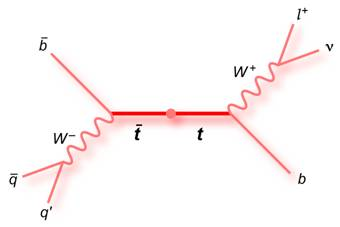
\includegraphics[width=0.5\textwidth]{TopAnalysis/figures/TopFeynmann.jpg}
  \caption[Semileptonic $t\bar{t}$ decay]{Semileptonic $t\bar{t}$ decay}
  \label{fig:topfeynmann}
\end{figure}

Here we give details of an analysis proposed for measuring the top quark forward-backward asymmetry, A$_{FB}^t$, at CLIC during the 1.4 TeV stage. 

As already described in Chapter \ref{theory}, A$_{FB}^t$ is sensitive to the electroweak form factors of the ttX(X=Z,$\gamma$) vertex. By measuring A$_{FB}^t$ and the $t\bar{t}$ cross section at multiple energies and with different beam polarizations it is possible to extract values for the electroweak form factors and use these as a probe for testing the \ac{SM} and searching for \ac{BSM} physics. This measurement is well motivated by the existing result for the b quark forward-backward asymmetry as measured at \ac{LEP}, which currently provides the largest deviation from the \ac{SM} within electroweak fits. Due to the limited energy at \ac{LEP} (which is still the highest energy e$^+$e$^-$ collider to have existed,) no analagous measurement of the asymmetry for tops has ever been performed at a lepton collider. 

\begin{table}
  \centering
  \begin{tabular}{l |c}
    \toprule
    Decay Mode     & Branching Fraction (\%) \\
    \midrule
    Fully Hadronic & 45.3  \\
    $tt\rightarrow WbWb\rightarrow qqbqqb$ & \\
    \midrule
    Semileptonic & 43.8 \\
    $tt\rightarrow WbWb\rightarrow qqbl\nu b$ &  \\
    \midrule
    Fully Leptonic & 10.6 \\
    $tt\rightarrow WbWb\rightarrow l\nu bl\nu b$ &  \\
    \midrule
    $tt\rightarrow Other$ & 0.4 \\
    \bottomrule
  \end{tabular}
  \caption{Top Pair Decay Modes}
  \label{table:topdecaymodes}
\end{table}

A$_{FB}$ is defined as:

\begin{equation}
A_{FB}^t=\frac{N_F-N_B}{N_F+N_B}
\end{equation}
Where N$_{F}$ and N$_{B}$ are the number of top quarks produced in the forward and backward directions which are defined to be the hemispheres corresponding to an angle of less than and greater than 90$^0$ relative to the direction of motion of the electrons initial momentum respectively.

As tops decay almost exclusively to a W and b (99.8\% of decays) they are typically described in terms of the resulting decay modes of the Ws. The dominant decay modes are described in \reftab{table:topdecaymodes}. Here we will look at measuring $A_{FB}^{t}$ using the semileptonic $t\bar{t}$ decay channel (see \reffig{fig:topfeynmann}) in which one of the W's decays to a lepton and neutrino and the other W decays to a a pair of quarks. This decay mode is ideal as the lepton from the leptonically decaying top provides the ability to charge tag the top while the fully hadronic decay allows an accurate measurement of the production angle of the top, both of which are necessary for measuring $A_{FB}^{t}$ to high precision. Due to the sensitivity of $A_{FB}^{t}$ to polarization states, the measurment will be done for two different electron beam polarizations, -80\% and +80\%, assuming an even split of luminosity between the two configurations. The dominant signal and background processed examined by this analysis, as well as their cross sections and production ID numbers for each polarization are shown in \reftabs{table:topsamplesnegpol} and \ref{table:topsamplespospol}. All samples are simulated using the CLIC\_ILD\_CDR detector model. This is a variation of the ILD detector model developed for use at the ILC. The samples also include an overly of $\gamma\gamma\rightarrow$ hadron events from beamstrahlung based on a 30~ns window around the generated physics events. Because these are inclusive sample, before they can be used for the analysis the $e^+e^-\rightarrow qqqql\nu$ samples must be filtered to extract the signal process. This is done by trying all combinations of $qqq$ and $ql\nu$ and seeing if there was any case in which the resulting particles both had masses within 5$\times\Gamma_t$ of $m_t$. Within the generator $m_t$ and $\Gamma_t$ are 174 GeV and 1.4 GeV respectively. In the case that two tops could not be classified, the event would be described as either single top or non top depending on whether any single combination off $qqq$ or $ql\nu$ was in the correct mass window. The dominant backgrounds are expected to be from alternative $t\bar{t}$ decays (fully hadronic decay modes and semileptonic decays containing taus) and from single top events (see \reffig{fig:singletop}) which will have very simliar topologies due to the fact they can both contain a hadronically decaying top.

\begin{figure}
  \centering
  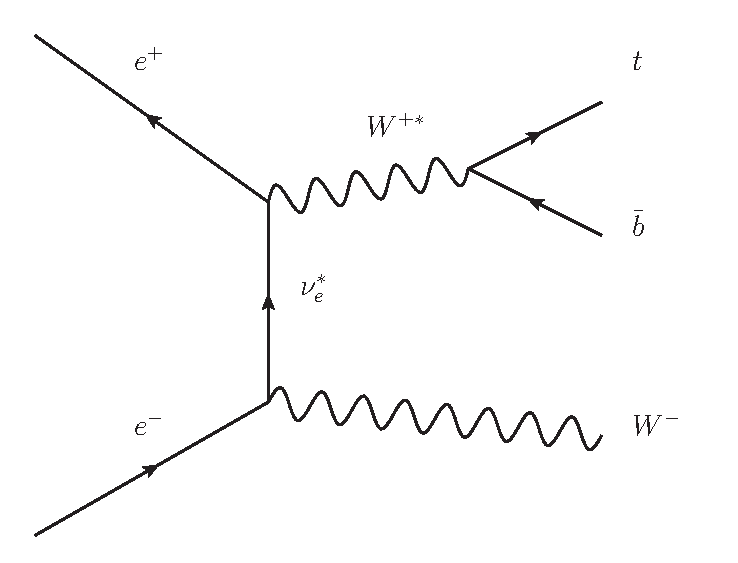
\includegraphics[width=0.5\textwidth]{TopAnalysis/figures/SingleTop}
  \caption[Dominant single top production mode]{Dominant single top production mode capable of mimicking the signal process}
  \label{fig:singletop}
\end{figure}

\begin{table}
  \centering
  \begin{tabular}{l | r | r |r}
    \toprule
    Process     & Cross Section(fb) & Production ID & Events Used (10$^{-3}$) \\
    \midrule
    $e^+e^-\rightarrow qqqql\nu$ & 142.3 & 6589,6592,6634,6637 & 3860 \\
    \midrule
    $e^+e^-\rightarrow qqqqqq$ & 116.4 & 6595, 6598, 6601, 6604,  & 310 \\
     &  & 6610, 6607, 6613, 6616,  &  \\
     &  &  6619, 6622  &  \\
    \midrule
    $e^+e^-\rightarrow qql\nu l\nu$ & 44.1 & 6586, 6625, 6628, 6631 & 100 \\
    \midrule
    $e^+e^-\rightarrow qqqq$ & 2304.0 & 8254 & 1,590 \\
    \midrule
    $e^+e^-\rightarrow qql\nu$ & 6975.0 & 7477 & 3,520 \\
    \midrule
    $e^+e^-\rightarrow qqll$ & 2681.0 & 8244 & 1,190 \\
    \midrule
    $e^+e^-\rightarrow qq\nu\nu$ & 1395.0 & 8271 & 1,120 \\
    \midrule
    $e^+e^-\rightarrow qq$ & 4843.0 & 8283 & 2,400 \\
    \bottomrule
  \end{tabular}
  \caption{Samples used in the -80\% electron beam polarization study}
  \label{table:topsamplesnegpol}
\end{table}

\begin{table}
  \centering
  \begin{tabular}{l | r | r |r}
    \toprule
    Process     & Cross Section(fb) & Production ID & Events Used (10$^{-3}$) \\
    \midrule
    $e^+e^-\rightarrow qqqql\nu$ & 53.5 & 6646, 6697, 6691, 6694 & 160 \\
    \midrule
    $e^+e^-\rightarrow qqqqqq$ & 44.9 & 6652, 6655, 6658, 6661, & 198 \\
     &  & 6664, 6667, 6670, 6673, &  \\
     &  & 6676, 6679 &  \\
    \midrule
    $e^+e^-\rightarrow qql\nu l\nu$ & 15.3  & 6643, 6682, 6685, 6688 & 15.3 \\
    \midrule
    $e^+e^-\rightarrow qqqq$ & 347 & 8257 & 500 \\
    \midrule
    $e^+e^-\rightarrow qql\nu$ & 1640 & 7480 & 1,000 \\
    \midrule
    $e^+e^-\rightarrow qqll$ & 2530 & 8241 & 1,000 \\
    \midrule
    $e^+e^-\rightarrow qq\nu\nu$ & 180 & 8274 & 200 \\
    \midrule
    $e^+e^-\rightarrow qq$ & 3170 & 8286 & 1,500 \\
    \bottomrule
  \end{tabular}
  \caption{Samples used in the +80\% electron beam polarization study}
  \label{table:topsamplespospol}
\end{table}


The results presented here are currently being included in a paper summarising the top physics potential at \ac{CLIC}, however this paper is still under review. Within the paper there is an alternative version of this analysis performed by Lars Rickard Str{\"o}m (CERN) in which an entirely different reconstruction and event selection is performed. The results of both analysis have been found to yield consistent results for the expected precision on $A_{FB}^{t}$ when accounting for differences in the expected signal efficiency. As the paper is still under review it is not possible to provide a reference to the finished document, however a full description of the alternative analysis can be found here (CITATION OF RICKARD).


\section{Event Reconstruction}
Reconstruction of the signal events is performed using ILCSOFT v01-17-10 and consists of three main stages. The first stage is to identify isolated leptons arising from the leptonically decaying top. These leptons are then removed and the remaining PFOs are resolved into two large radius ``fat jets''. These two fat jets must then be associated with either the b jet produced by the leptonically decaying top or to the combination of three jets arrising from the hadronically decaying top. A kinematic fitter is then used to reconstruct the neutrino and any \ac{ISR}/\ac{BS} photons present in the event. Throughout the analysis only tight selected PFOs have been considered in the reconstruction (PFOs reconstructed using with a timing cut of $\sim$ 2ns placed on clusters in the detector\cite{cdrvol2}) so as to reduce beam backgrounds.

\subsection{Lepton Finding}

Lepton finding is the first stage of reconstruction performed in each event. Due to the fact the measurement of $A_{FB}^{t}$ is entirely reliant on using the lepton charge to distinguish between top and antitop decays, it is essential that a high efficiency and purity are achieved and that there is no angular dependence on the performance. For this analysis lepton finding is done in two steps. Firstly, lepton candidates with energy $>$ 10~GeV are identified using the particle ID provided by the Pandora Particle Flow Algorithm \cite{Thomson200925}. Only muons and electrons are examined due to the fact tau leptons require different reconstruction techniques to identify and are typically reconstructed with significantly lower efficiency. This first stage removes $>$ 90\% of fake candidates with negligible impact on efficiency. The second stage of lepton selection is to examine how isolated each of the candidates are. This is evaluated by resolving all PFOs in the event into five jets, then for each lepton candidate measuring the energy of the candidate relative to the jet it was been associated with. For this process the inclusive ee kt algorithm was chosen for the jet finding to ensure that all lepton candidates are always placed within a jet. The lepton candidate found to have the highest ratio of $E_{Candidate}/E_{Jet}$ is then declared to be the isolated lepton arrising from the letonically decaying top. In the event that no lepton is selected by the first step, the restrictions on the particle ID and energy are relaxed and the lepton is selected purely based on which PFO is the most isolated according to step two. This method ensures that there is always exactly one lepton selected per event. The net efficiency with which this method selects a candidate with the correct charge is found to be 93\% for electrons and 96\% for muons.

As well as understanding the net efficiency for finding leptons it is also important to examine the angular dependence of the efficiency to ensure there is no bias that could effect the measurement of $A_{FB}^{t}$. \reffig{fig:netefficiency} shows how the efficiency varies with angle. The efficiency is seen to rapidly decline for $|Cos\theta| > 0.9$ due to detector acceptances. A decrease in efficiency is also seen for electrons at angles corresponding to the transition point between the ECAL barrel and endcaps. This effect is not seen for muons as they are also reconstructed using the muon detectors placed at a larger radius. Overall the efficiency is seen to be consistently worse for electrons than muons. This is to be expected as muons produce easily recognisable signatures in the detector due to the fact they typically penetrate through the tracker, ECAL, HCAL and muon sytems whereas electrons only leave deposits in the tracker and ECAL. In the case that tracks are lost during reconstruction or are wrongly associated to other PFOs it is then possible for photons to wrongly be labelled as electrons and vice versa leading to a higher fake rate for electrons.

\begin{figure}
  \centering
  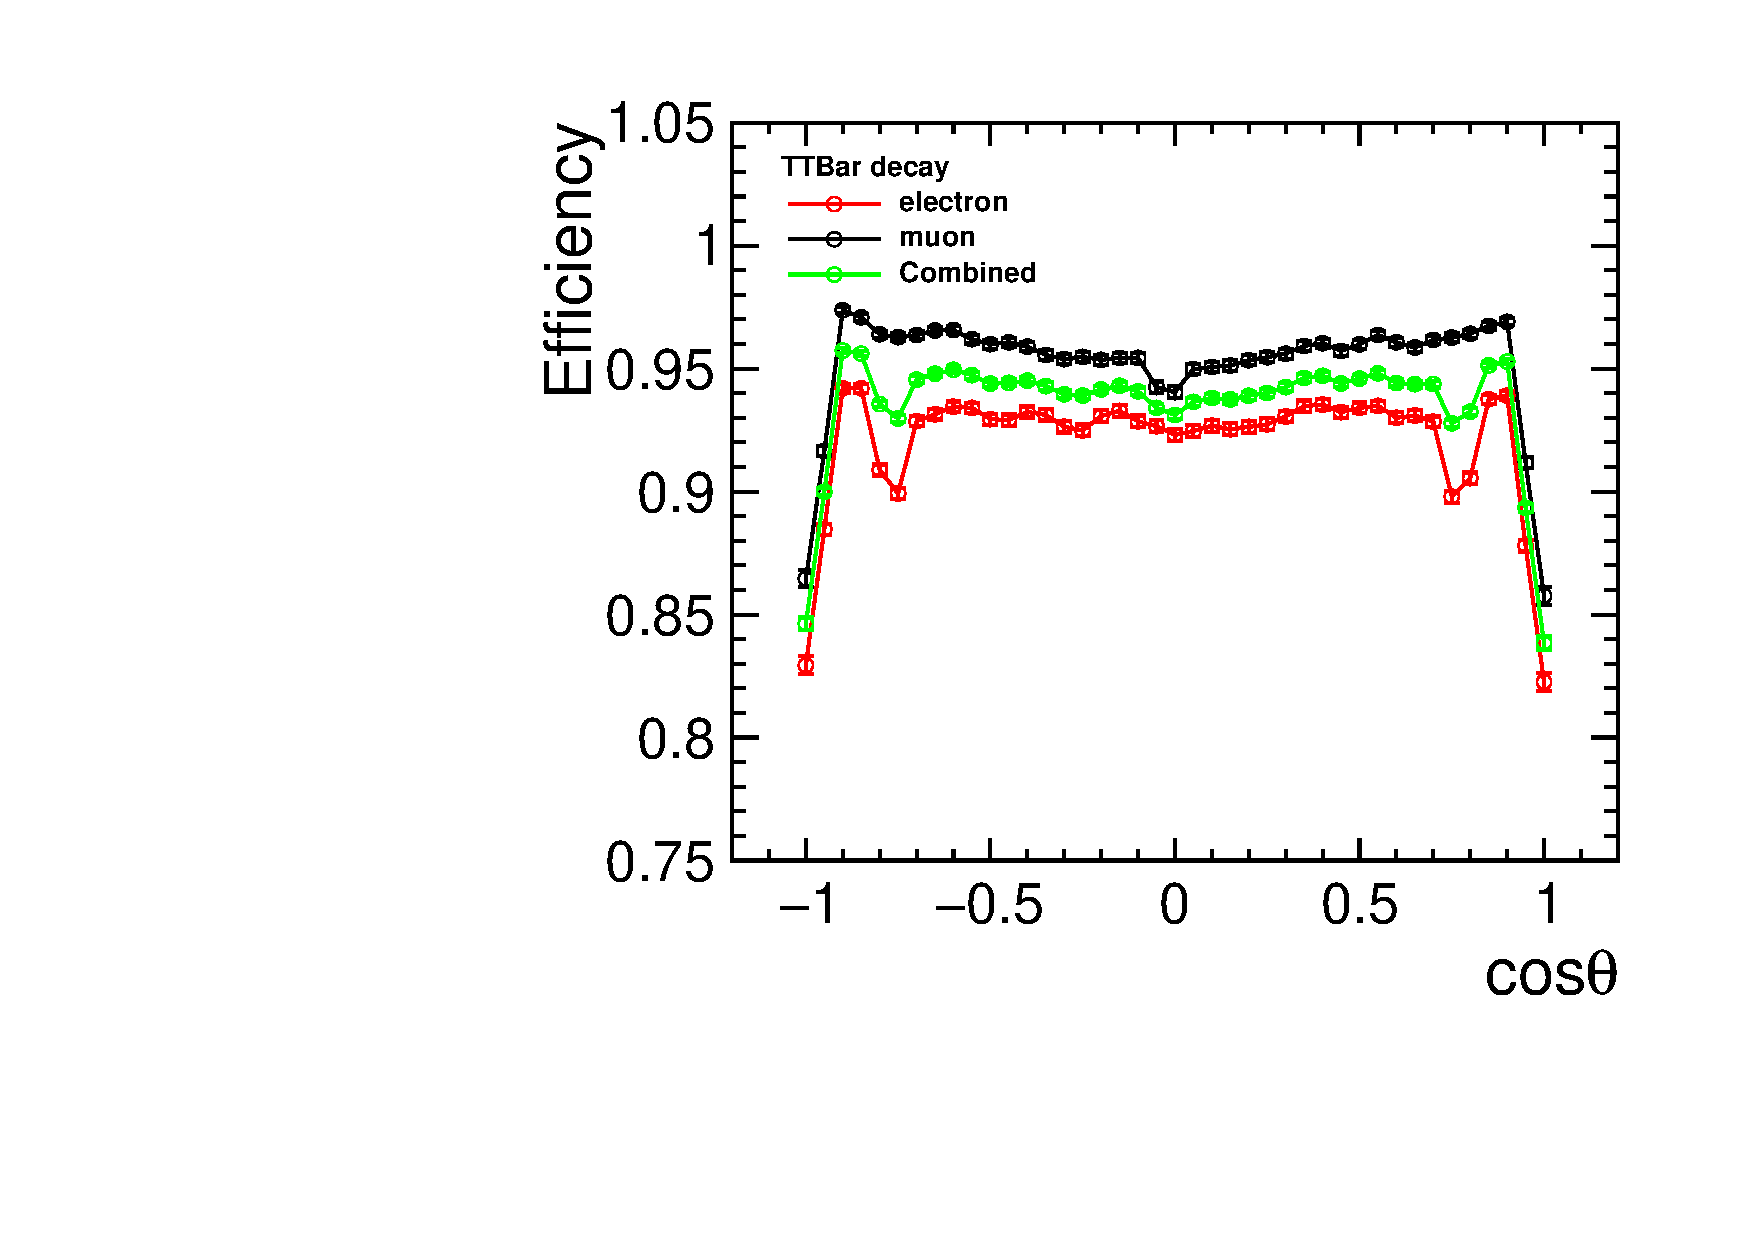
\includegraphics[width=0.6\textwidth]{TopAnalysis/figures/NetEfficiencys.pdf}
  \caption[Charge Tagging Efficiency]{Efficiency for identifying leptons with the correct charge as a function of angle}
  \label{fig:netefficiency}
\end{figure}

As well as checking the angular dependence of the charge tagging efficiency it is also key to examine the charge dependence of the lepton finding to make sure there is no preference for identifying particles over antiparticles. The angular dependence of the charge tagging efficiency for particles vs antiparticles is shown in \reffig{fig:chargeEfficiencies}. An asymmetry in the performance is observed in both electrons and muons.

\begin{figure}
  \centering
  \begin{subfigure}{.5\textwidth}
    \centering
    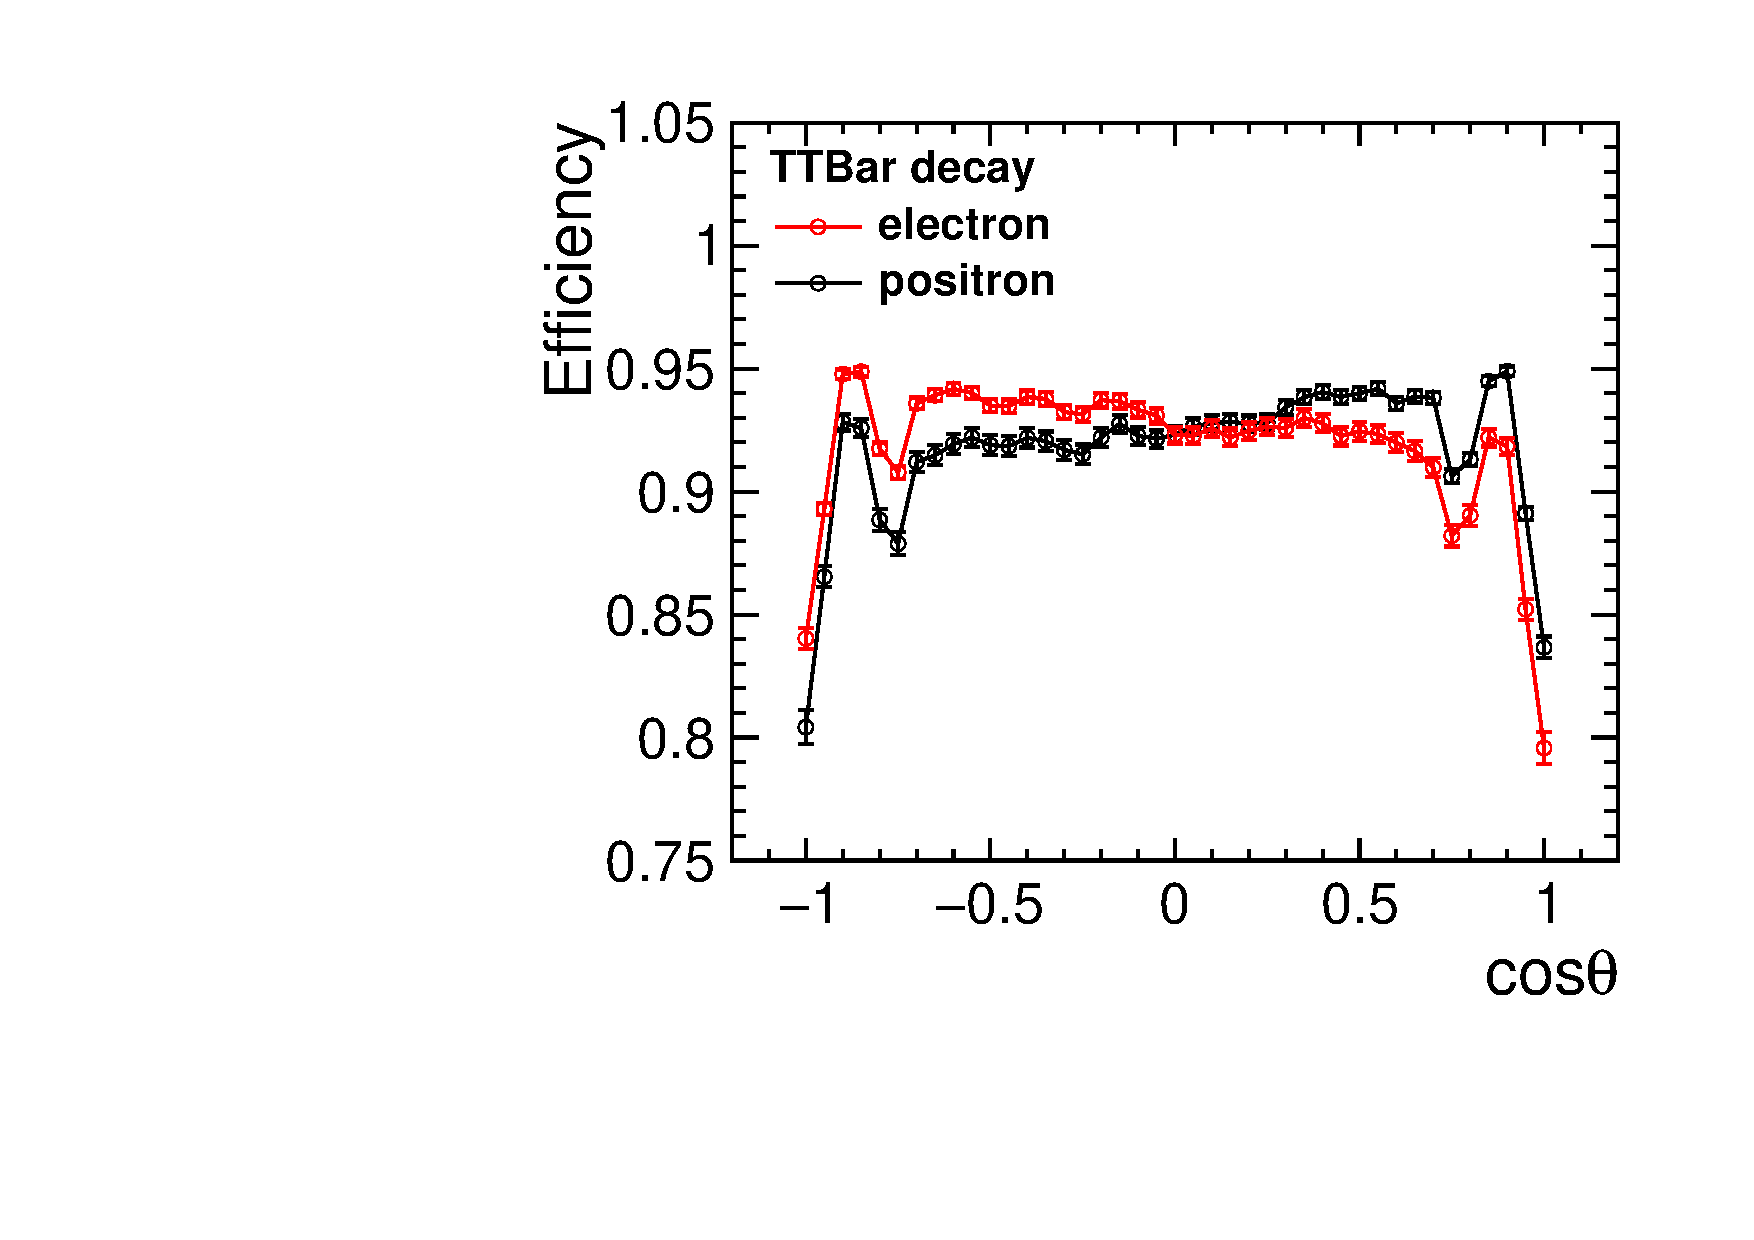
\includegraphics[width=0.9\textwidth]{TopAnalysis/figures/ElectronEfficiencys.pdf}
    \caption[Charge Tagging Efficiency]{Electrons}
    \label{fig:electronefficiency}
  \end{subfigure}%
  \begin{subfigure}{.5\textwidth}
    \centering
    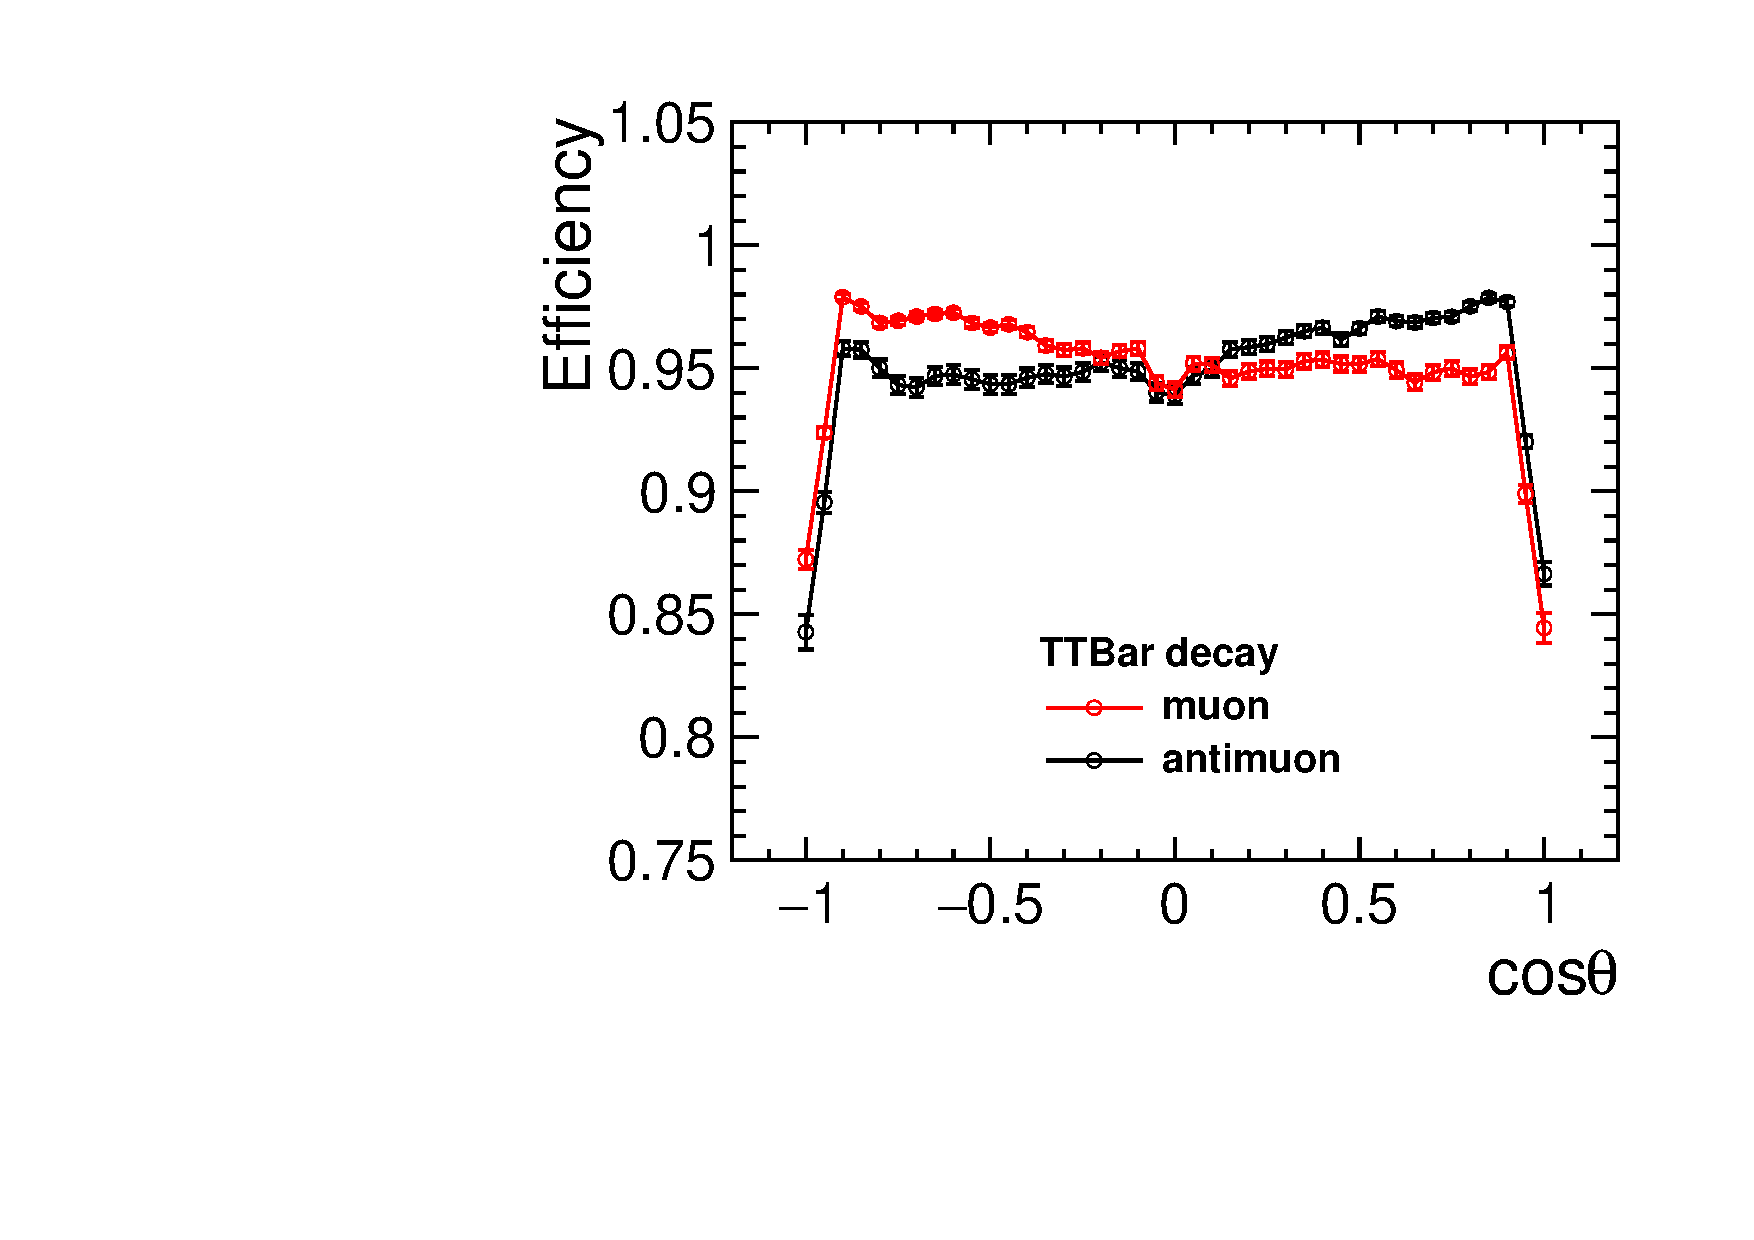
\includegraphics[width=0.9\textwidth]{TopAnalysis/figures/MuonEfficiencys.pdf}
    \caption[Charge Tagging Efficiency]{Muons}
    \label{fig:muonefficiency}
  \end{subfigure}
  \caption{Angular dependence of lepton finding for particles vs antiparticles}
  \label{fig:chargeEfficiencies}
\end{figure}

It arises from the underlying asymmetry in the production of particles vs antiparticles due to forward-backward asymmetries. The forward backward asymmetry means that tops are preferencialy produced in one direction while antitops are produced more often in othe opposite direction, however due to charge conservation this also means that the W bosons and leptons are produced asymmetrically too. Because the collisions are taking place well above the top pair production threshold, the W bosons will gain a large boost forcing them to travel in the same direction as the inital top. The polarization of the W also means that the lepton will also be preferencially produced along the same diection as the W and can only be produced in the opposite direction with a lower energy. Overall this means that leptons are produced with higher energy in one direction and lower energy in the opposite direction while for antileptons this directional dependence is reversed. The effect is shown in \reffig{fig:efficiency2d} where it is seen that positrons are produced with higher energy in the forward direction($cos\theta>0$) than the backward direction. It is known that the efficiency for reconstructing leptons at CLIC increases with energy and so the fact the energy and angle at which leptons are produced are correlated results in the asymmetric angular efficiency for correctly reconstructing the lepton. Further evidence for this theory is shown in \reffig{fig:higgsleptons} and \ref{fig:effienciesWithCuts} which show that the asymmetry disappears when either the production mode for the leptons is symmetric or when low energy leptons are not included.

\begin{figure}
  \centering
  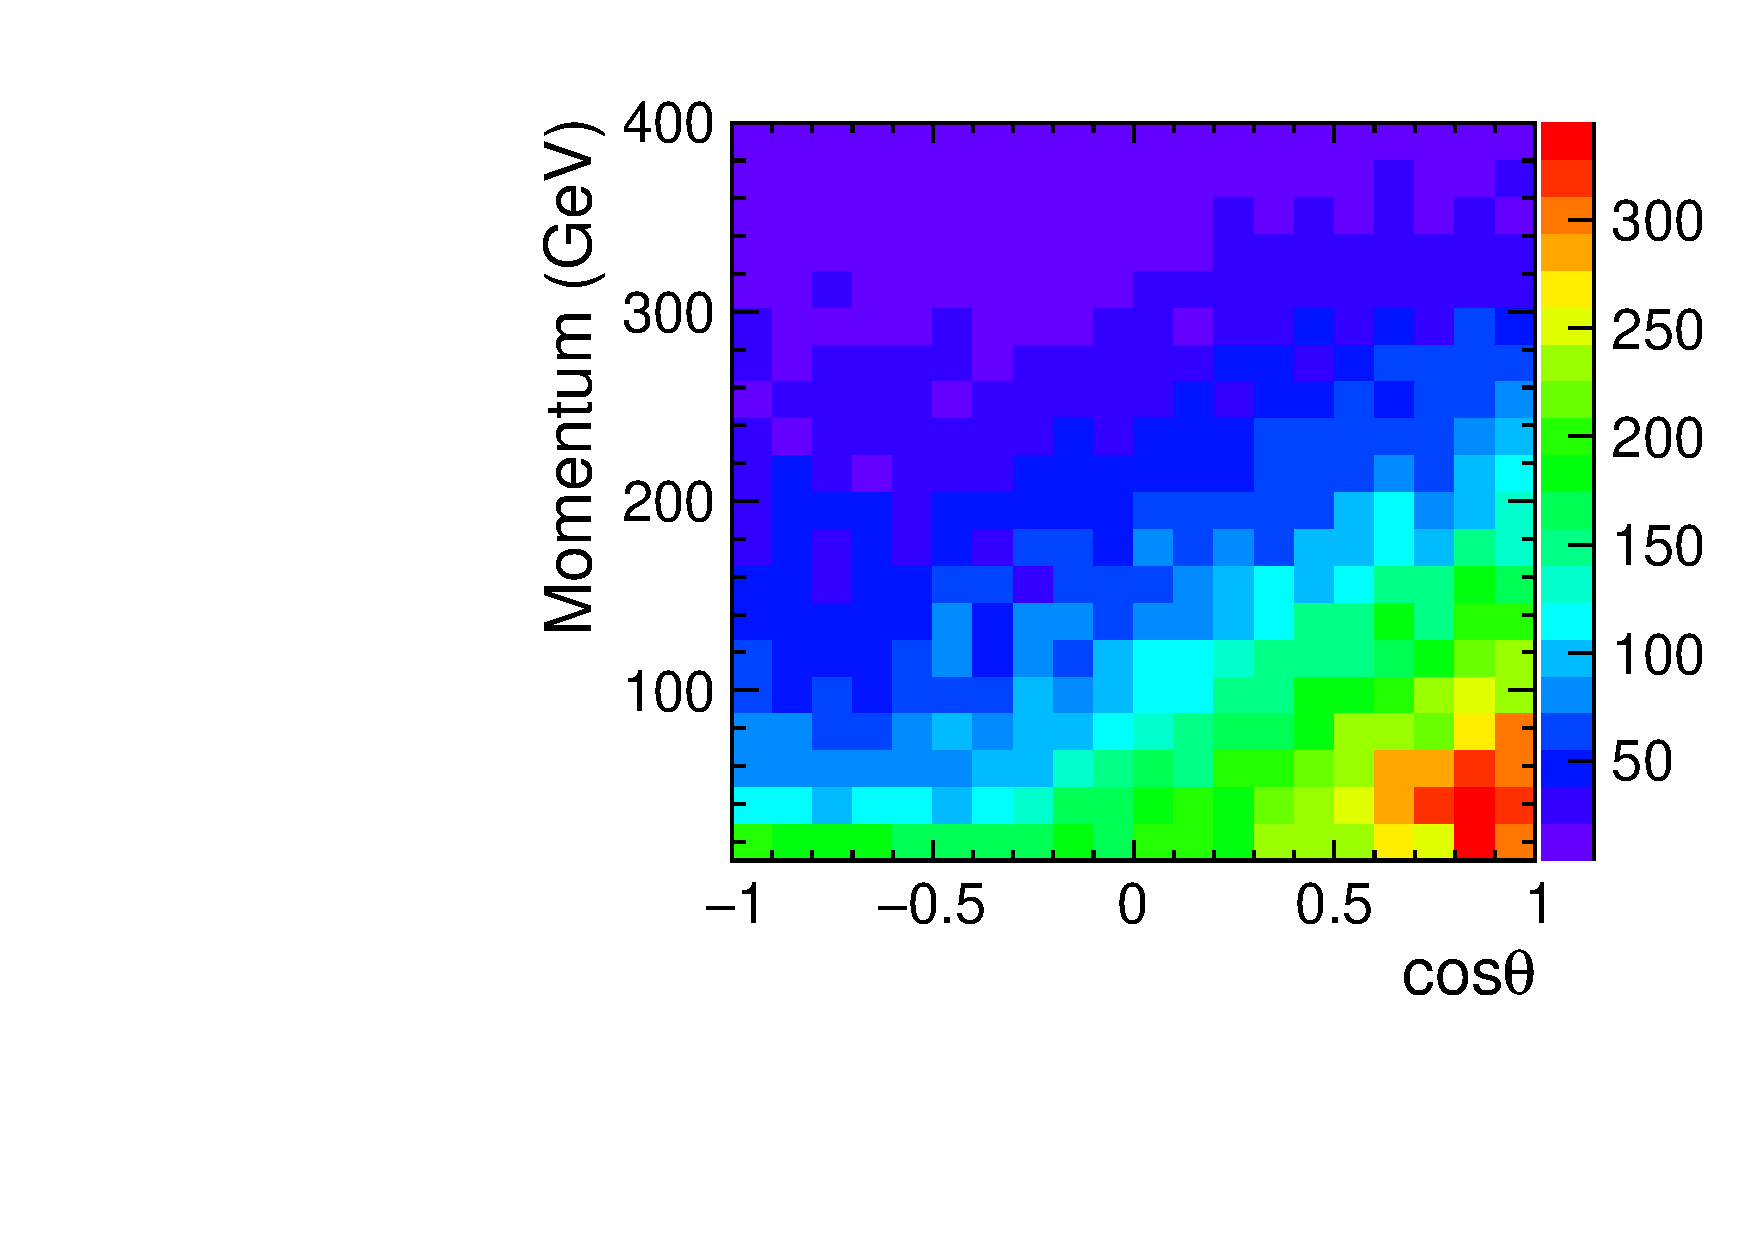
\includegraphics[width=0.6\textwidth]{TopAnalysis/figures/MomentumVsTheta.pdf}
  \caption[Lepton Momentum Vs Angle]{Correlation between lepton momentum and angle for positrons only}
  \label{fig:efficiency2d}
\end{figure}

\begin{figure}
  \centering
  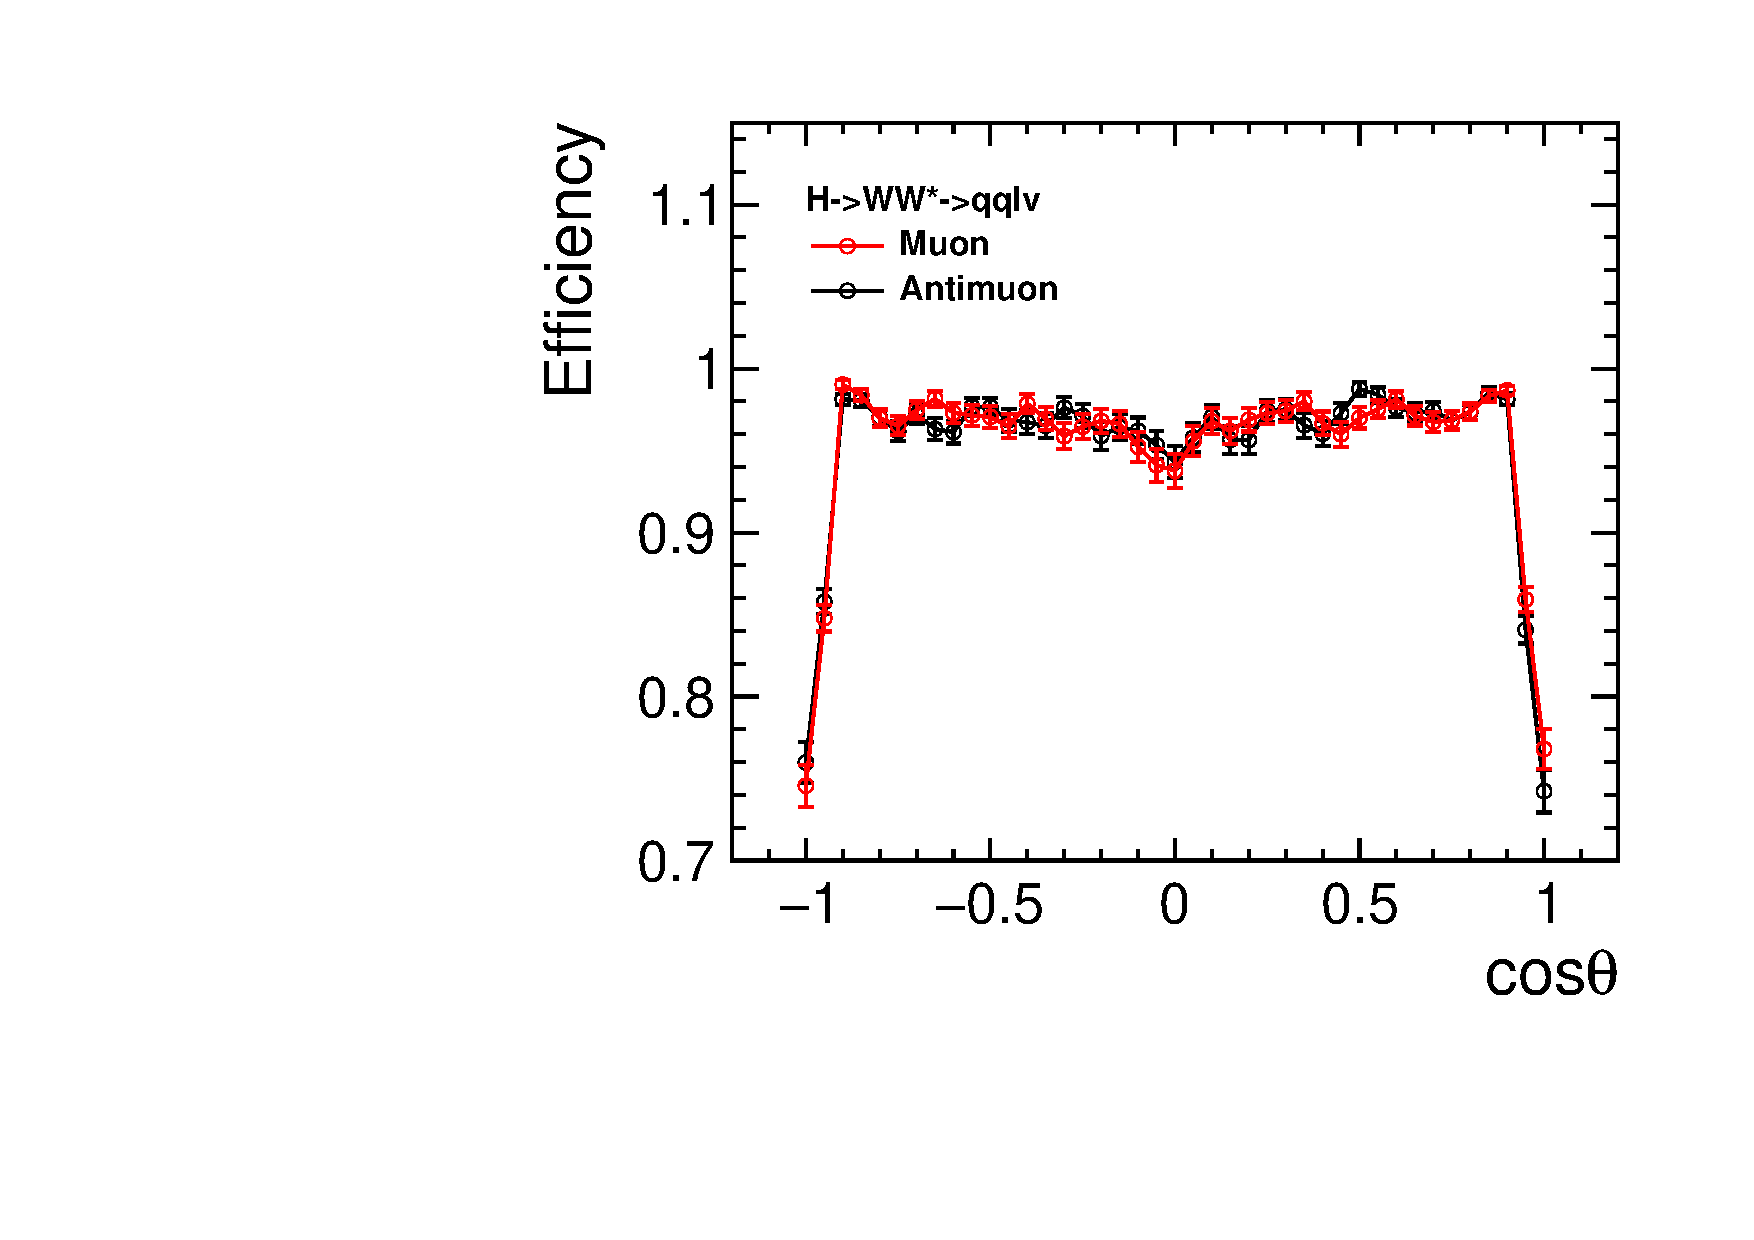
\includegraphics[width=0.6\textwidth]{TopAnalysis/figures/MuonEfficiency_Higgs.pdf}
  \caption[Lepton efficiency for $ee\rightarrow H\nu\nu,H \rightarrow WW\rightarrow qql\nu$ ]{Charge tagging efficiency for $ee\rightarrow H\nu\nu,H \rightarrow WW\rightarrow qql\nu$. The efficiency is seen to be symmetric for particles and antiparticles when they are produced with the same initial angular distribution.}
  \label{fig:higgsleptons}
\end{figure}

\begin{figure}
  \centering
  \begin{subfigure}{.5\textwidth}
    \centering
    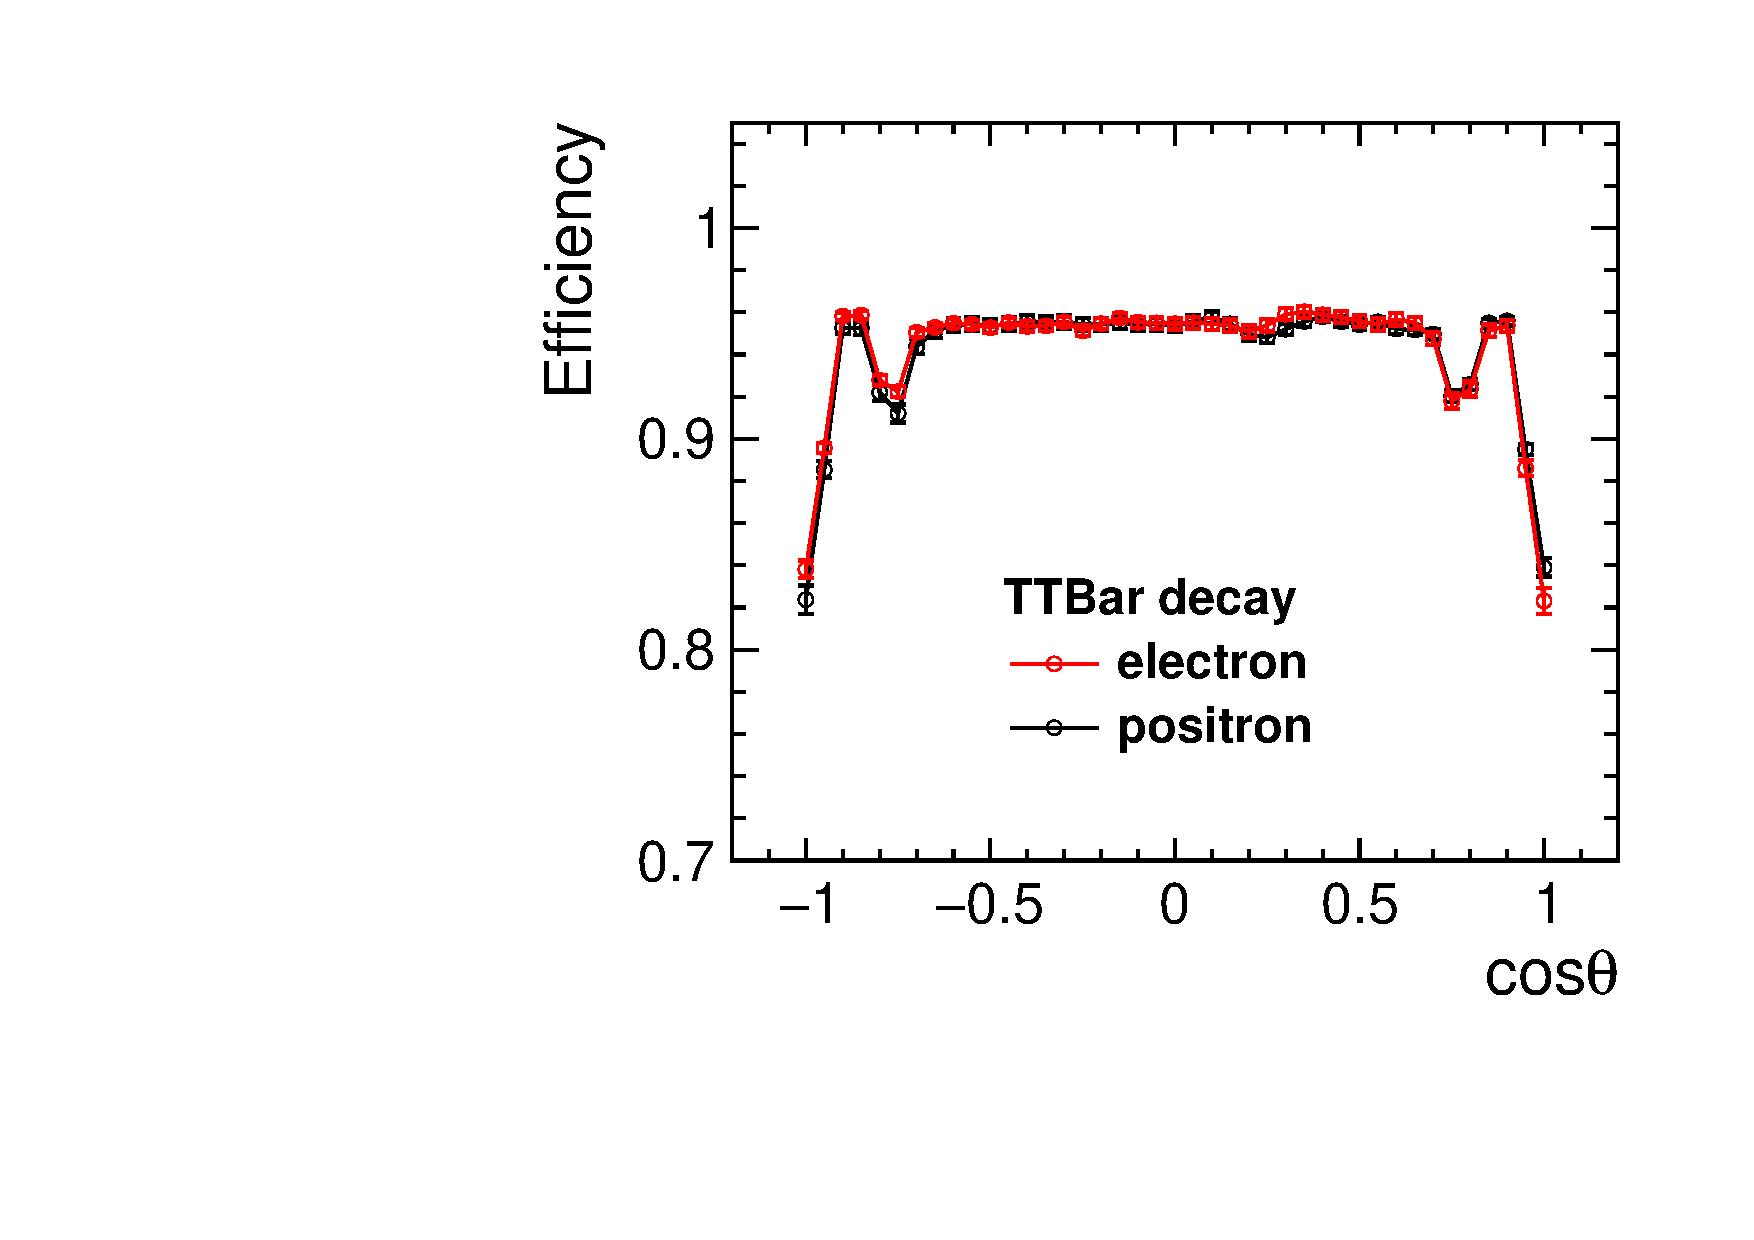
\includegraphics[width=0.9\textwidth]{TopAnalysis/figures/ElectronEfficiencys_20GeVMCCut.pdf}
    \caption[Charge Tagging Efficiency]{Electrons}
  \end{subfigure}%
  \begin{subfigure}{.5\textwidth}
    \centering
    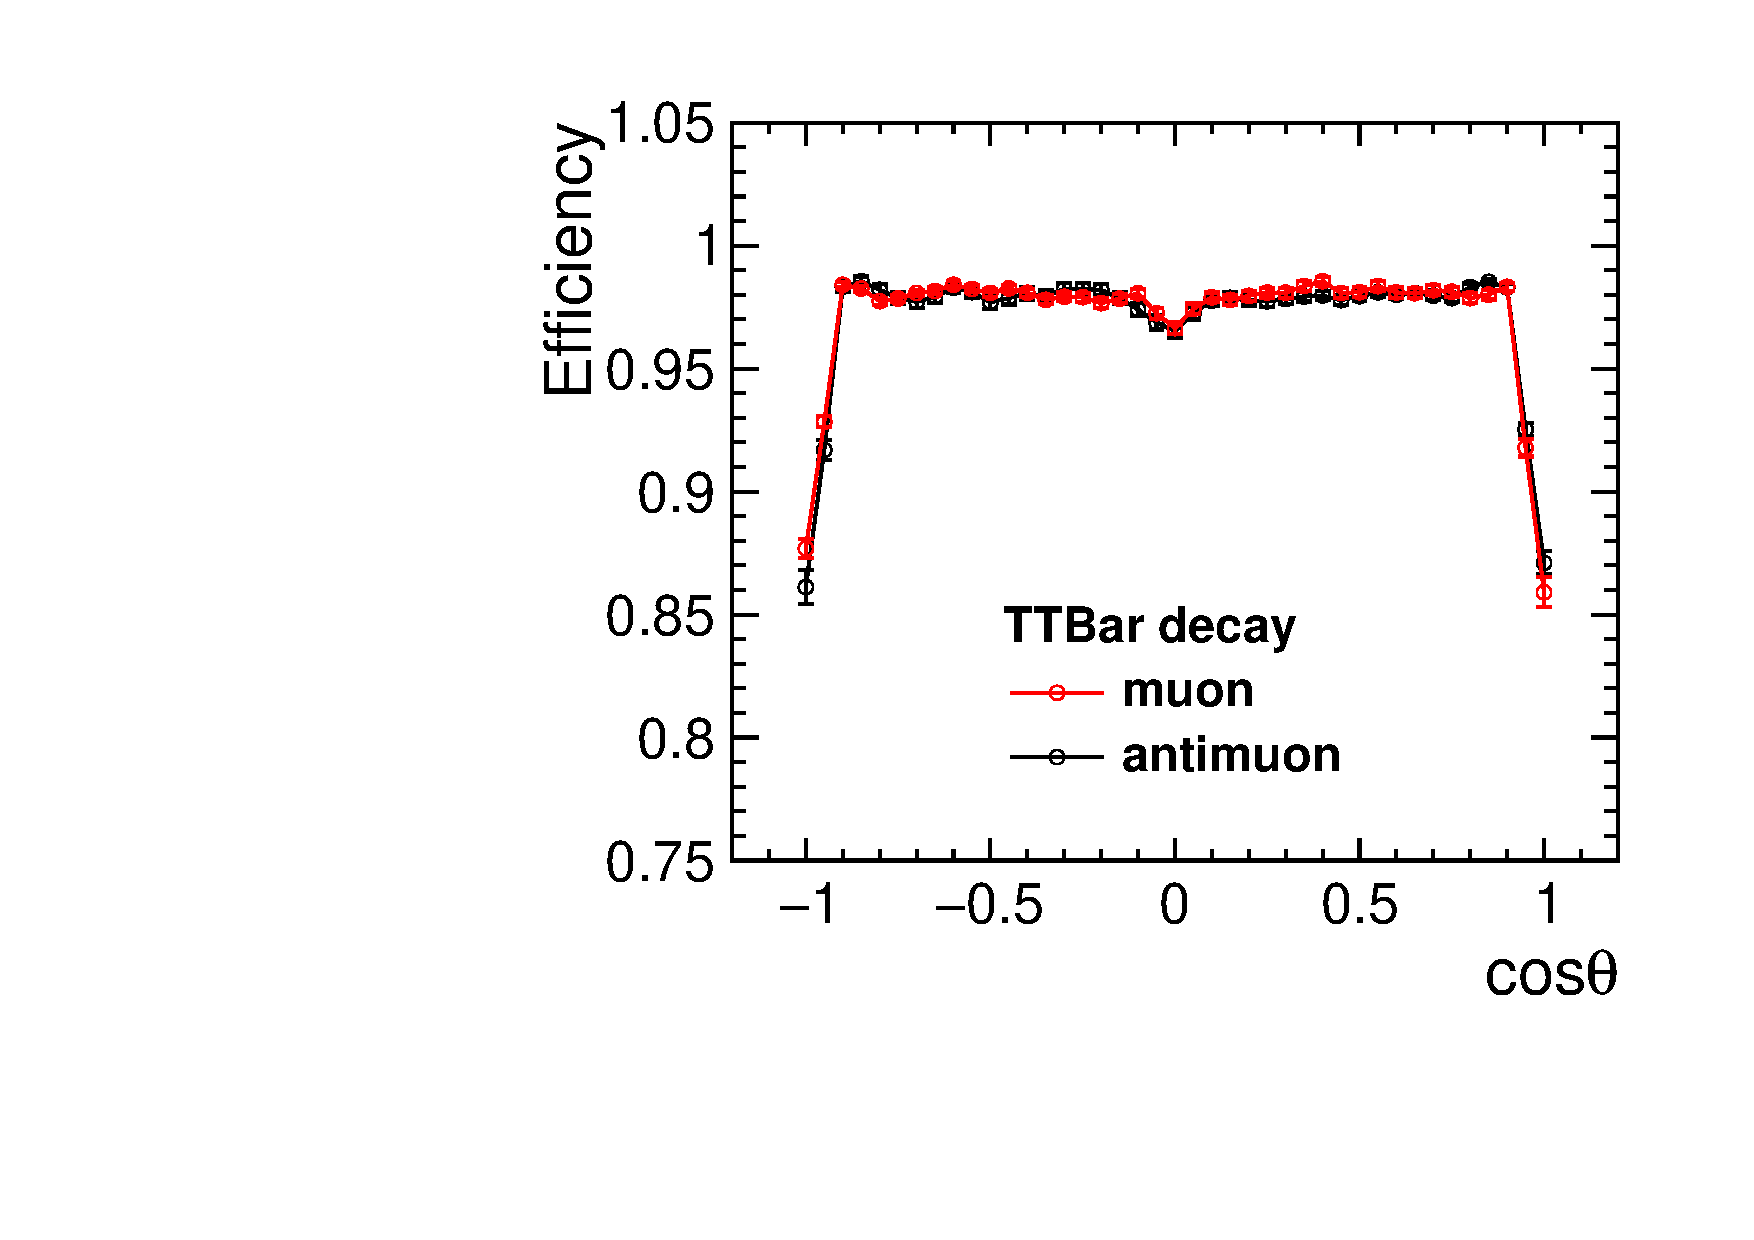
\includegraphics[width=0.9\textwidth]{TopAnalysis/figures/MuonEfficiencys_20GeVMCCut.pdf}
    \caption[Charge Tagging Efficiency]{Muons}
  \end{subfigure}
  \caption[Charge Tagging Efficiency After 20GeV Lepton Momentum Cut]{Charge tagging efficiency after 20~GeV lepton momentum cut. The efficiency is seen to be symmetric for leptons with momentum $>$ 20~GeV}
  \label{fig:effienciesWithCuts}
\end{figure}


\subsection{Fat Jet Finding}

\begin{figure}
  \centering
  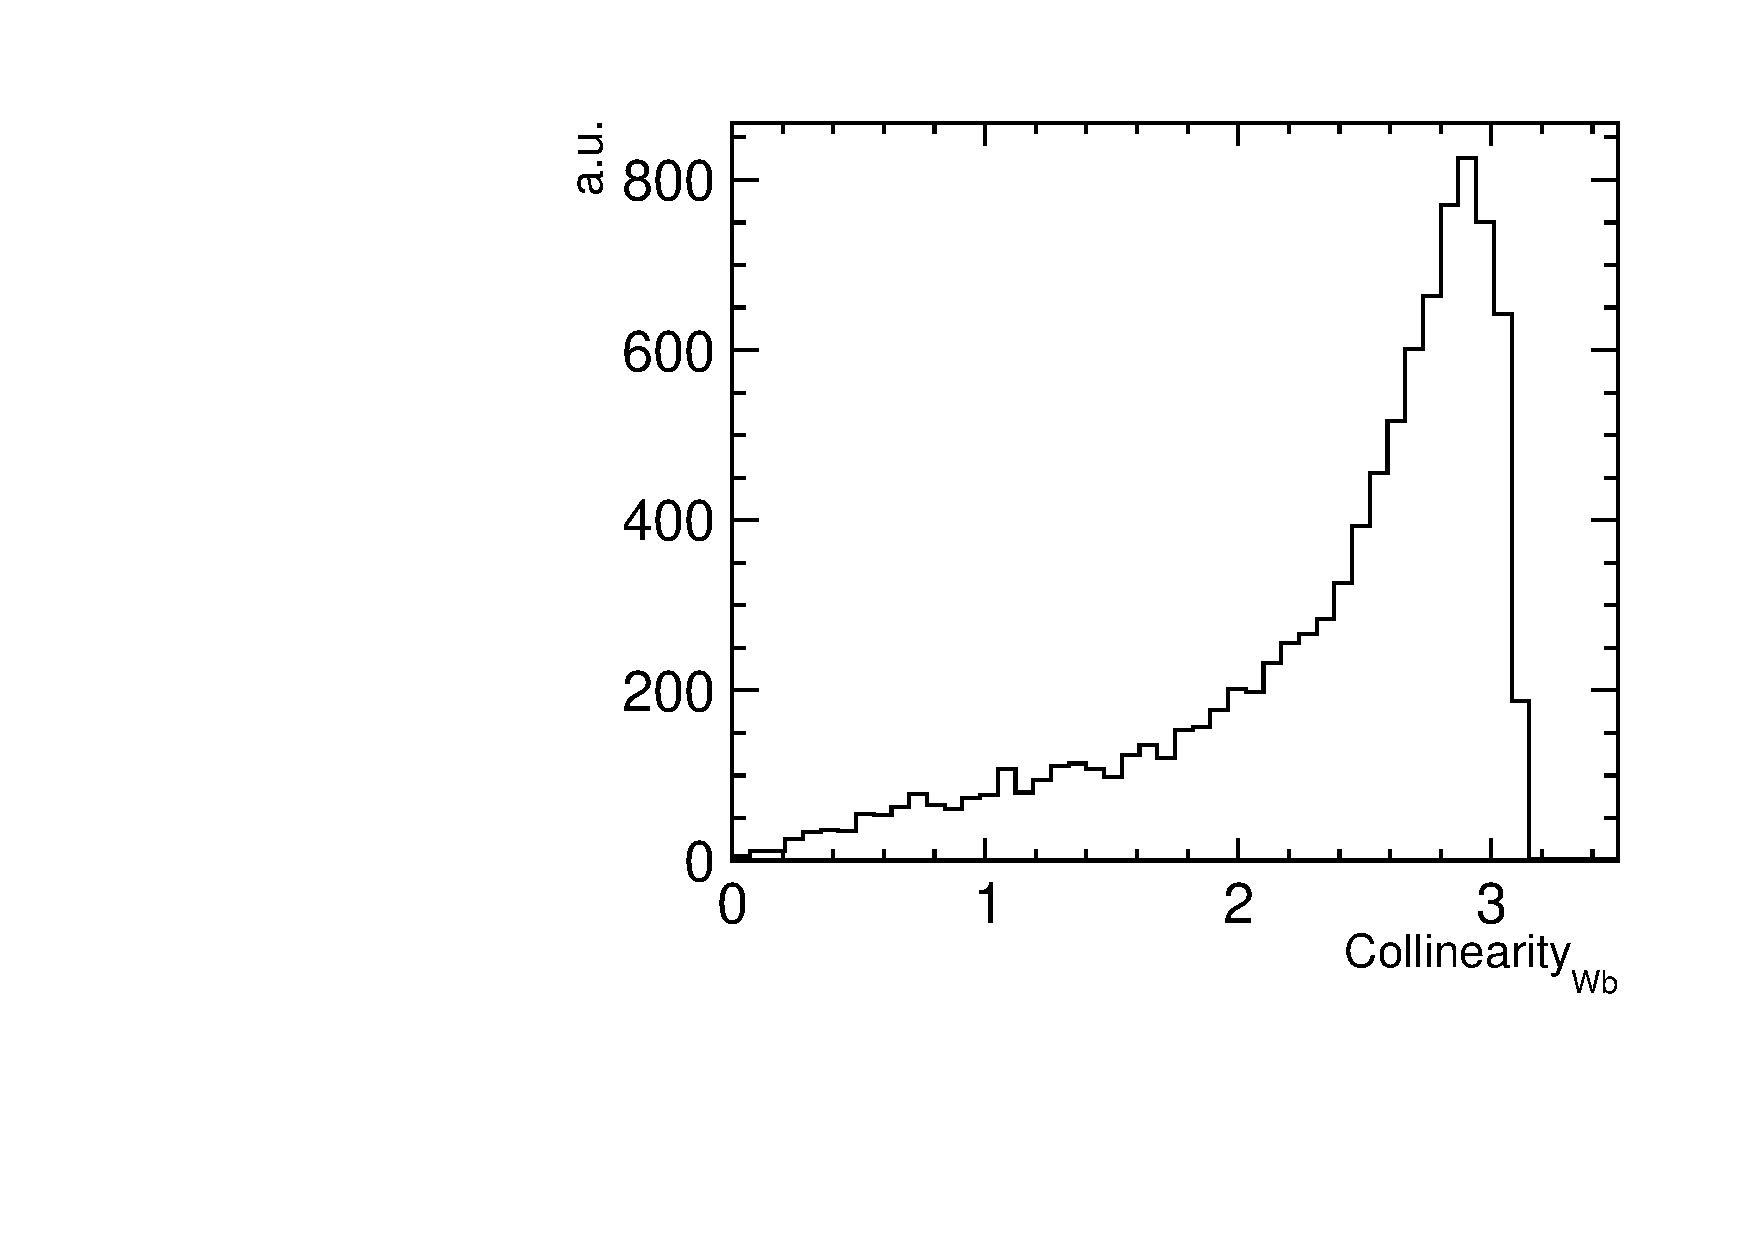
\includegraphics[width=0.6\textwidth]{TopAnalysis/figures/WBCollinearity.pdf}
  \caption[Separation between W and b jet from top decay]{Separation between W and b jets from top decay. The pair are typically too collimated to allow the b-jet and the pair of jets from the W decay to be successfully resolved into three distinct jets}
  \label{fig:Collimated}
\end{figure}

Jet reconstruction was performed using the FastJet package \cite{Cacciari:2011ma}. Due to the high energy of the collisions relative to the top mass, the tops produced are highly boosted and produce highly collimated decay products (see \reffig{fig:Collimated}.) This means it is typically not possible to resolve the decay products from the hadronically decaying top into three jets corresponding to the b-jet and light quark jets from the W decay. As a result an alternative approach to jet reconstruction is considered based on the concept of fat jets, an approach already being used at the LHC\cite{Miller:2011qg}. Fat jets are large radius jets and are used to cluster groups of jets that can't be accurately resolved individually into one larger jet. For the purpose of this anaylsis the events are clustered into fat jets which should correspond to the b-jet from the leptonically decaying top and to the whole set of decay products from the hadronically decaying top. The mass and substructure variables (see \refsec{Event Selection}) of these fat jets can then be used to distinguish genuine top events from backgrounds. Two jet algorithms were considered for reconstructing the fat jets- the longitudinally invaraint kt algorithm \cite{Cacciari:2008gp} and Valencia algorithm \cite{Boronat:2014hva}. The kt algorithm is already extensively used at hadron colliders while the Valencia algorithm is a newer algorithm designed for future lepton colliders that offers improved performance in handling beam backgrounds. A full description of the kt algorithm is already given in \refsec{higgsjetfinding} so here we will only describe the Valencia algorithm. Overall the Valenica algorithm is similar to the kt algorithm, however the key differences are that the inter-particle distance and beam distance are redefined as:

\begin{equation}
d_{ij}=min(E_i^{2\beta},E_j^{2\beta})(1-cos\theta_{ij})/R^2
\end{equation}
\begin{equation}
d_{iB}=p_T^{2\gamma}E^{2(\beta - \gamma)}
\end{equation}

Where R is the usual jet radius defined in the same way as for the kt algorithm and $\beta$ and $\gamma$ are additional parameters that can be used to tune how the algorithm behaves for particles approaching the beam line. \reffig{fig:valenciaPerformance} shows how the ratio $d_{ij}/d_{iB}$ develops for a pair of particles produced with fixed energy and angular separation as a function of their polar angle for multiple $\beta$ factors. One can see that a higher $\beta$ factor introduces a larger penalty for approaching the beam line leading to an decreased chance for the particles to be merged into a jet.

\begin{figure}
  \centering
  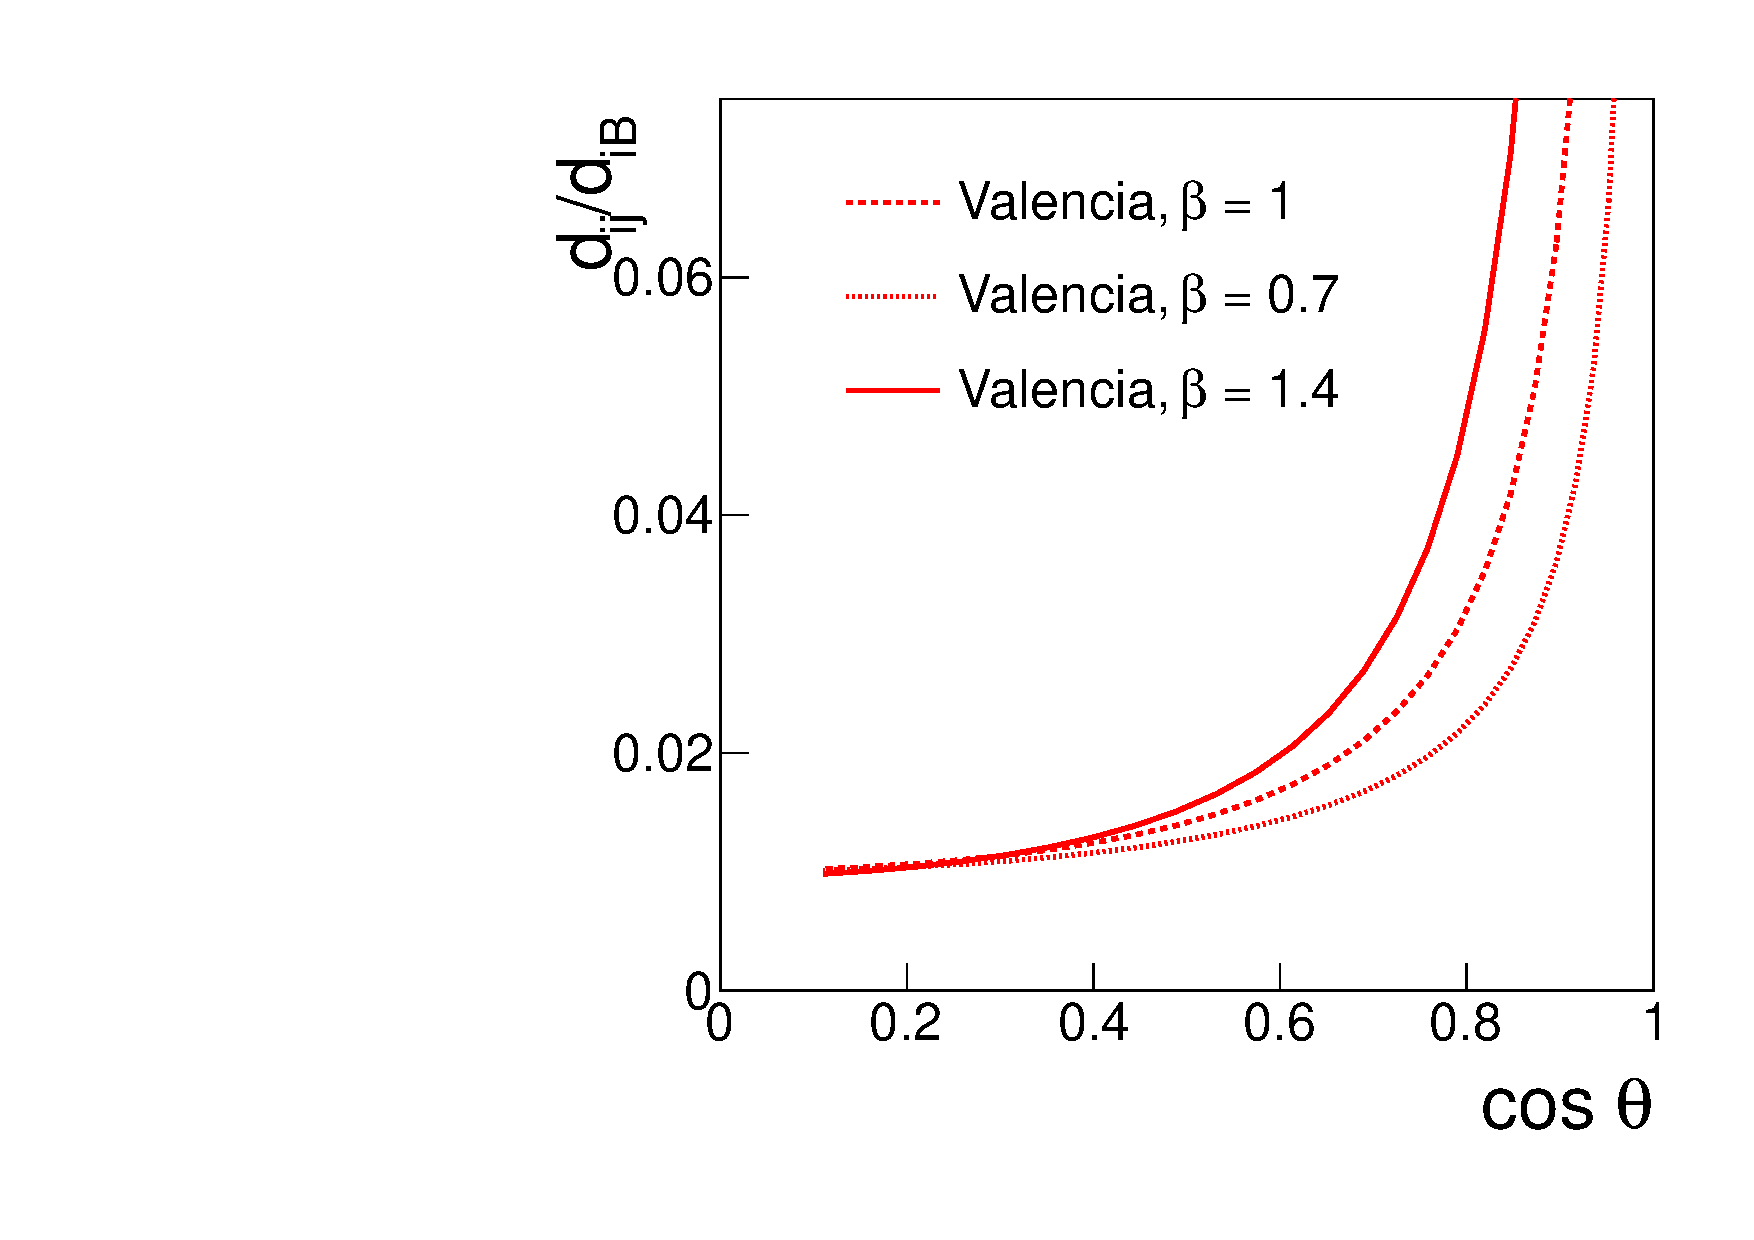
\includegraphics[width=0.6\textwidth]{TopAnalysis/figures/distance_ratio_vlc.pdf}
  \caption[Effect of the Valencia $\beta$ parameter]{Effect of the Valencia $\beta$ parameter on $d_{ij}/d_{iB}$ for a pair of particles produced at a fixed energy and angular separation as a function of their polar angle\cite{Boronat:2014hva}}
  \label{fig:valenciaPerformance}
\end{figure}

The performance of both algorithms is shown in figure \reffig{fig:jetfinding}. For both algorithms it is seen that at higher R the resolution on the top mass gets worse while for lower R sub-peaks start to appear in the mass distribution corresponding to partial reconstructions of the top (either a W Boson or single quark). The kt algorithm is seen to produce a consistently broader distribution in the top mass. Placing a cut on the collision energy of E $>$ 1.2~TeV reveals that these lower mass peaks only occur for lower collision energies where the tops will no longer be produced back to back and their decay products will be less collimated. As a result the fat jet finding can merge components from both the hadronic and leptonic tops into each jet. This analysis will be focusing on reconstructing the most boosted tops. As a result the Valencia algorithm is preferred due to it's better mass resolution. Performance for less boosted top decays might be improved by examining the performance of a more conventional jet analysis looking to resolve all four individual quarks whenever the fat jet finding produces jets outside the top mass window. This possibility is discussed later in \refsec{Quality Cuts}. Here the Valencia algorithm with R=1.5, $\beta$=1 and $\gamma$=1 is chosen as the optimal jet reconstrcution method to provide a balance between mass resolution and the frequency of partial reconstructions. 

\begin{figure}
  \centering
  \begin{subfigure}{.5\textwidth}
    \centering
    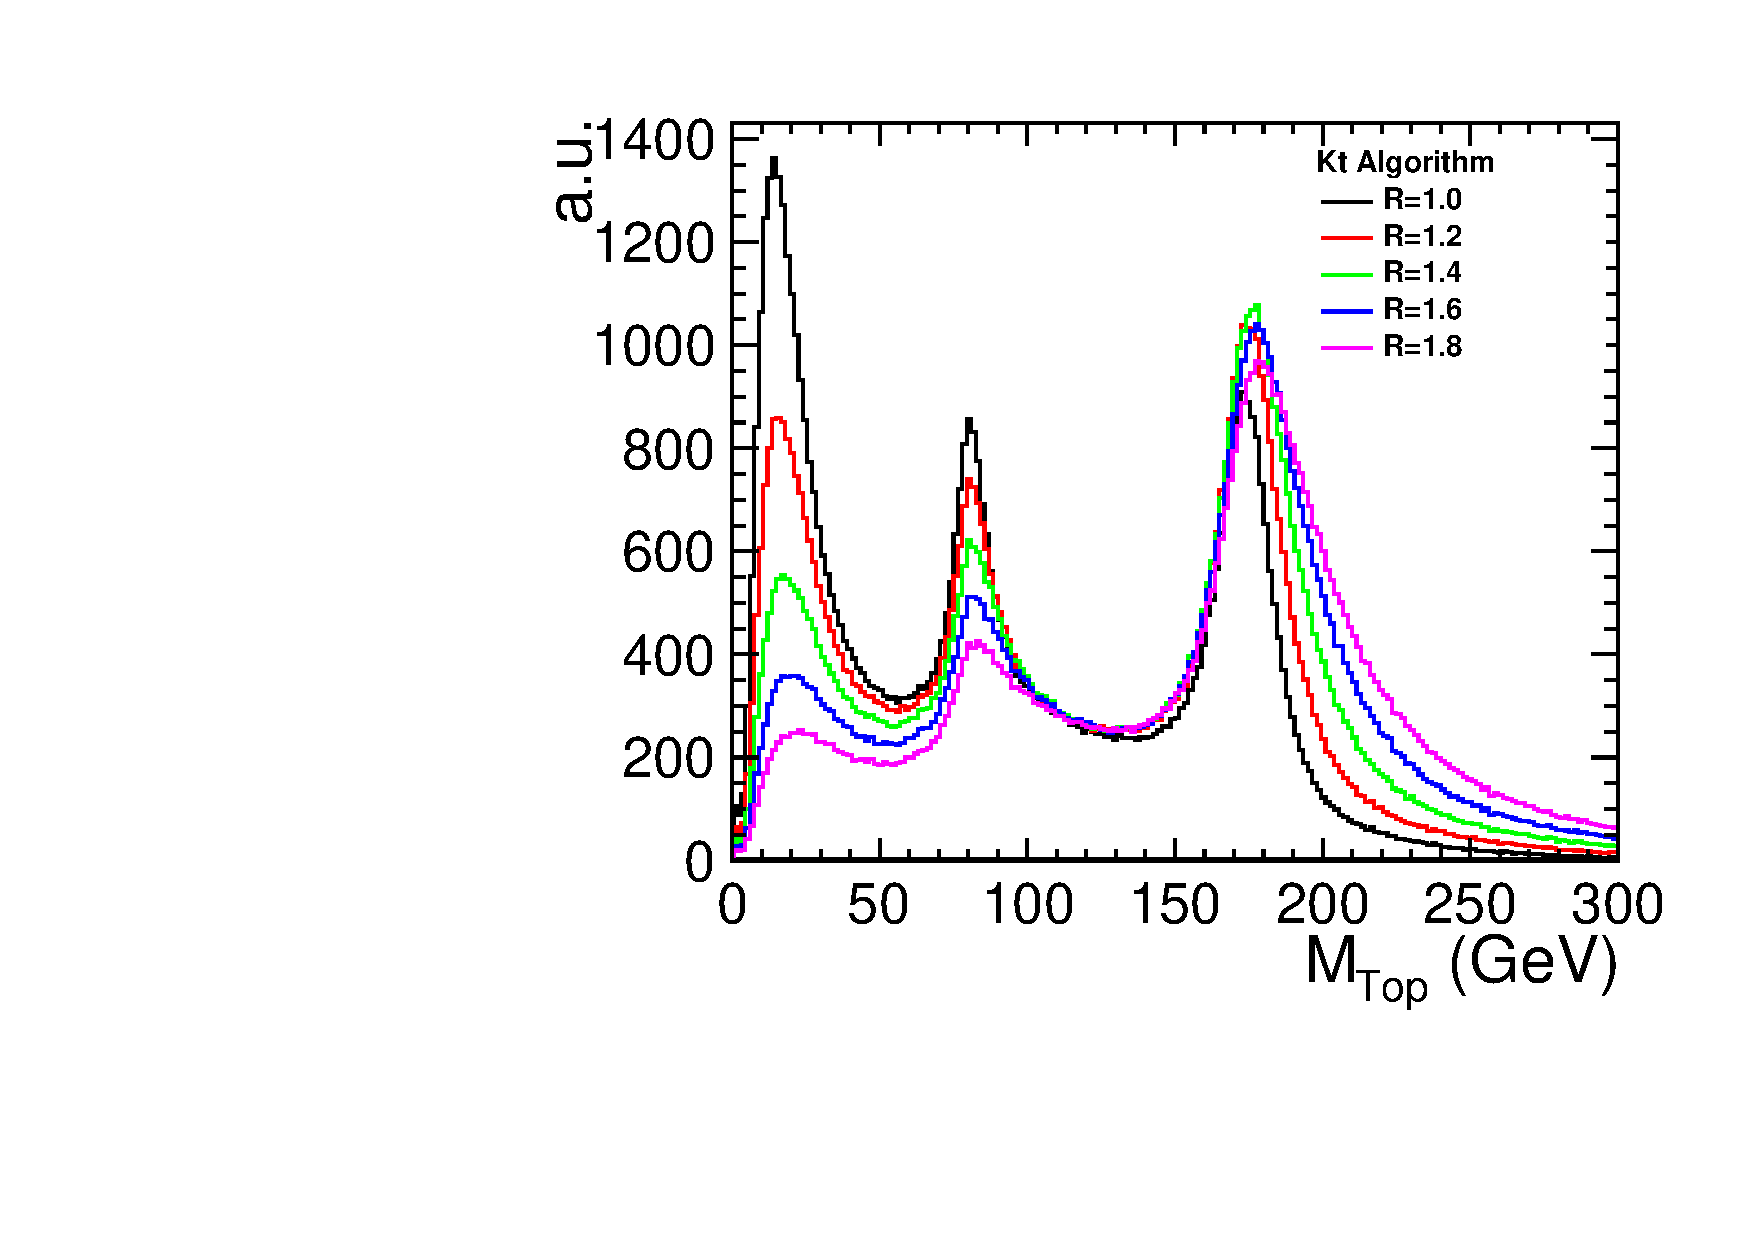
\includegraphics[width=1.0\textwidth]{TopAnalysis/figures/ComparisonKt.pdf}
    \caption[kt algorithm]{kt algorithm}
  \end{subfigure}%
  \begin{subfigure}{.5\textwidth}
    \centering    \includegraphics[width=1.0\textwidth]{TopAnalysis/figures/ComparisonVLC.pdf}
    \caption[Valenica algorithm]{Valencia algorithm}
  \end{subfigure}
  \caption[Performance of jet finding algorithms]{Performance of both jet finding algorithms for various parameter settings. The kt algorithm is seen to produce a broader distribution in the top mass peak so the Valencia algoritm is prefered. For both methods it is seen that a lower R results in the development of peaks from partial reconstruction of the top jet (W Boson or single quark) while a larger R produces a broader peak at the top mass. A balance is found between producing a narrow top mass width while minimising sub peaks by selecting a radius of R=1.5 }
  \label{fig:jetfinding}
\end{figure}


\begin{figure}
  \centering
  \includegraphics[width=0.7\textwidth]{TopAnalysis/figures/TopMass_EOver1200.pdf}
  \caption[Performance of Valencia algorithm for high energy events]{Reconstructed top mass for the Valencia algorithm in events close to the nominal collison energy (E $>$ 1.2~TeV)}
  \label{fig:highEValencia}
\end{figure}


\subsubsection{Jet Association}
\label{sec:jetassociation}
\begin{figure}
  \centering
  \includegraphics[width=0.7\textwidth]{TopAnalysis/figures/CosThetaRecoVsMC.pdf}
  \caption[Comparison of reconstructed top decay angle to generator level]{Comparison of reconstructed top decay angle to generator level. A strong correlation is seen over most of the range, however this starts to break down for large angles of $\mid cos\theta \mid>0.9$ where non-negligible off diagonal contributions are seen.}
  \label{fig:2djetangle}
\end{figure}

\begin{figure}
  \centering
  \begin{subfigure}{.5\textwidth}
    \centering
    \includegraphics[width=1.0\textwidth]{TopAnalysis/figures/TopMassDiagonal.pdf}
  %  \caption[$\mid\frac{cos\theta_{Reco}}{cos\theta_{Generator}}\mid >1$]{Fat jet mass when $\mid\frac{cos\theta_{Reco}}{cos\theta_{Generator}}\mid >1$, on diagonal regions of fig \ref{fig:2djetangle}.}
  \end{subfigure}%
  \begin{subfigure}{.5\textwidth}
    \centering\captionsetup{width=.8\linewidth}%
    \includegraphics[width=1.0\textwidth]{TopAnalysis/figures/TopMassOffDiagonal.pdf}
 %   \caption[$\mid\frac{cos\theta_{Reco}}{cos\theta_{Generator}}\mid >1$]{Fat jet mass when $\mid\frac{cos\theta_{Reco}}{cos\theta_{Generator}}\mid <1$, off diagonal regions of fig \ref{fig:2djetangle}.}
  \end{subfigure}
  \caption[Reconstructed fat jet mass]{Reconstructed fat jet mass. In the on diagonal elements of \reffig{fig:2djetangle}) where $\mid\frac{cos\theta_{Reco}}{cos\theta_{Gen.}}\mid >1$ (left) the reconstructed fat jet matches the top mass, while in the regions corresponding to the off diagonal regions of \reffig{fig:2djetangle}) (right) the mass is no longer consistent.}
  \label{fig:diagonalTopMass}
\end{figure}


After the fat jet finding has been performed, the two reconstructed jets must then be associated as either coming from the hadronically decaying top or from the b jet from the leptonically decaying top. The default method for this was to associate the highest energy fat jet to the hadronically decaying top as, due to the neutrino not being reconstructed and the lepton already being removed, the remaining decay products from the leptonically decaying top should typically have considerably less energy. The performance of this method can be examined by comparing the reconstructed decay angle relative to the generator value (see \reffig{fig:2djetangle}). While the performance over most of the range studied is good, for $\mid cos\theta \mid>0.9$ the correlation between the generator and reconstructed angles breaks down and off diagonal elements start to appear. Performance in these forward regions is typically poor due to the detector acceptance which result in losses down the beam line. In cases where parts of the hadronic top decay are not able to be reconstructed, using the fat jets energy to perform the jet association no longer becomes a reliable method. Evidence that misreconstruction is the source of these off diagonal elements is presented in \reffig{fig:diagonalTopMass} where it is clear that the fat jets in the off diagonal regions are not reconstructed with a consistent mass. When the jets are not fully reconstructed, it is more likely that the wrong jet is assigned to be from the hadronic top. When the wrong jet is selected the reconstructed angle will be approximately $\pi$ radians off the generator value as the tops are predominantly produced back to back. This explanation is further supported by the results shown in \reffig{fig:2djetangle_farfromleptop} which show that the off diagonal elements can be removed when a cut is placed on the angle between the reconstructed top and the generator level b jet from the leptonic top decay indicating that these elements are definitely coming from selecting the wrong jet being selected. As well as the $\pi$ radian flips from selecting the wrong jet, there are also additional off diagonal contributions seen which arise from poor reconstruction of the fat jets. This typically happens when the tops are not produced back to back due to \ac{ISR}/\ac{BS}. When this happens, during the fat jet reconstruction it is possible for contributions from both true fat jets to be mixed e.g instead of grouping the 3 jets from the hadronic jets together only two of them are grouped together and the third is grouped with the lone b jet from the leptonic top. When this mismatching happens the hadronic top is no longer fully reconstructed and so the angle measured for the top decay has little correlation with the generator value. \reffig{fig:2djetangle_goodtopseparation} shows that these remaining off diagonal elements disappear when a cut is placed on the separation of the tops at truth level. 

\begin{figure}
  \centering
  \begin{subfigure}{.48\textwidth}
    \centering
    \includegraphics[width=1.0\textwidth]{TopAnalysis/figures/CosThetaRecoVsMC_NotNextToLepTop.pdf}%
    \caption[Cut placed on angle between reconstructed top and generator b jet from leptonic decay]{Cut placed on angle between reconstructed top and generator b jet from leptonic decay, $\Delta Cos\theta_{Reco-Bjet}>0.1$}
    \label{fig:2djetangle_farfromleptop}
  \end{subfigure}\hfill
  \begin{subfigure}{.48\textwidth}
    \centering
    \includegraphics[width=1.0\textwidth]{TopAnalysis/figures/CosThetaRecoVsMC_MCTopsWellSeparated.pdf}%
    \caption[Cut placed on collinearity between top pair at generator level]{Cut placed on collinearity between top pair at generator level, separation $>$ 3 radians}
    \label{fig:2djetangle_goodtopseparation}
  \end{subfigure}
  \caption[Reconstructed vs generator top decay angles with truth level cuts]{Reconstructed vs generator top decay angles with truth level cuts to explain the off diagonal elements seen in \ref{fig:2djetangle}.}
  \label{fig:2djetangle_explanations}
\end{figure}


In order to avoid the problems close to the beam line multiple alternative jet association methods were devised- see \reftab{tab:methodDescription}.
\begin{table}
  \centering
  \begin{tabular}{l |p{100mm}}
    \toprule
    Fat Jet Selection Method     & Description  \\
    \midrule
    Lepton & The hadronically decaying top is deemed to be the fat jet with the greatest angular separation from the isolated lepton\\
    \midrule
    B tag & The hadronically decaying top is deemed to be the fat jet with the greatest angular separation from the jet with the highest b tag (see \ref{Flavour Tagging} for details on how flavour tagging is performed)\\
    \midrule
    Energy & Select the fat jet with the highest energy to be the hadronically decaying top\\
    \midrule
    Multiplicity & Recluster both fat jets into N ``micro jets'' (see \ref{Jet Multiplicity} for methodology) The hadronically decaying top should have a higher number of micro jets found within it\\
    \midrule
    Mass & The hadronically decaying top is deemed to be the fat jet with the greatest mass \\
    \midrule
    Top Mass & Select the fat jet whos mass is closest to the top mass as the hadronically decaying top \\
    \midrule
    Democratic & A combination of the lepton, energy and mass methods. Each method votes for which fat jet it thinks is the hadronically decaying top. The fat jet with the most votes is then selected as the hadronically decaying top  \\
    \bottomrule
  \end{tabular}
  \caption{Methods used for identifying which fat jet corresponds to the hadronically decaying top.}
  \label{tab:methodDescription}
\end{table}

The relative effectiveness of these methods were evaluated in three ways shown in \reffigs{fig:methodComparison}, \ref{fig:angleFitDiff} and \ref{fig:angularEfficiency} respectively. The first method was to look at the overall distribution of cos$\theta$ produced by each method compared to the distribution at generator level as this is what will be used to extract $A_{fb}^{t}$. All the methods agree well with the generator distribution in the central region of the detector but diverge in the high $\mid cos\theta\mid$ region. This is mainly caused by the effect described above. Close to the beam line the jets aren't fully reconstructed, the jet association fails and the b jet from the leptonic side is selected rather than the hadronic top jet. This causes migrations from the forward region to the backward regions producing a deficit in the forward region and an excess in the backward region. Migrations do occur in the opposite direction too for the same reason, however because the top forward-backward asymmetry means tht more tops are produced in the forward region to begin with, the net migration is from forward to backward. The migrations are not always a shift of $\pi$ radians as one might expect. Instead the migrations occur from very close to the beam line to a broader range in the opposite direction. This is due to the fact that \ac{ISR}/\ac{BS} can mean the top pair aren't produced exactly back to back in the lab frame and because the b-jet produced by the leptonic decay is not exactly collinear with the the top decay axis. Comparing the methods we see that all the methods show similar levels of migration except for the btag method which shows the highest migration. This is attributed to the fact the highest btagged jet can sometimes be from the hadronic side even in events that are well reconstructed, and so the jet association will fail in more events than the other methods which only fail for events close to the beam line.

\begin{figure}
  \centering
  \includegraphics[width=0.6\textwidth]{TopAnalysis/figures/comparejetmethods.pdf}
  \caption[Reconstructed cos$\theta$ distribution for various jet association methods]{Reconstructed cos$\theta$ distribution for various jet association methods. The expected distribution from truth level information is uncluded for reference.}
  \label{fig:methodComparison}
\end{figure}

The second method was to measure the difference between the reconstructed and MC(generator) cos$\theta$ per event and fit this with a gaussian. The variation in the width and mean of these distributions were plotted against the generator cos$\theta$ and are shown in \reffig{fig:angleFitDiff}. The effects of migration at high cos$\theta$ is more pronounced in these plots where in the width we can see that the resolution on cos$\theta$ gets much worse in the forward regions and the mean shows a pull in opposite directions in these regions proving the migrations do indeed occur in both directions with the same rate. Unfortunately there is little discrimination seen between the methods except for showing that there are slightly larger migrations when using the b-tag method.

\begin{figure}
  \centering
  \begin{subfigure}{.5\textwidth}
    \centering
    \includegraphics[width=0.9\textwidth]{TopAnalysis/figures/MeanThetaDiff.pdf}
    \caption[Mean]{Mean}
  \end{subfigure}%
  \begin{subfigure}{.5\textwidth}
    \centering
    \includegraphics[width=0.9\textwidth]{TopAnalysis/figures/WidthThetaDiff.pdf}
    \caption[Width]{Width}
  \end{subfigure}
  \caption[Mean and width from fitting $\Delta cos\theta_{Gen.-Reco.}$ to a gaussian]{Mean and width from fitting $\Delta cos\theta_{Gen.-Reco.}$ to a gaussian. Mean: migrations close to $\mid cos\theta\mid>0.9$ result in a bias in the mean. The migrations cause a shift of roughly $\pi$ radians resulting in the bias being in the opposite direction for each end of the range. Width: migrations close to $\mid cos\theta\mid>0.9$ cause a broadening in the resolution of the reconstructed cos$\theta$.}
  \label{fig:angleFitDiff}
\end{figure}

The final method of comparison was to measure the efficiency with which the hadronic top was measured within the correct cos$\theta$ bin as a function of the generator cos$\theta$. For this study a bin width of 0.1 in cos$\theta$ was used. The results are shown in \reffig{fig:angularEfficiency}. Here there is a clearer separation in the performance of the different methods. B-tagging is seen to provide the worst efficiency while the energy and democratic methods provide the highest level of performance. The mass based selections provide slightly lower performance than the energy/democratic methods. This is likely explained by the fact they are less robust when the the event the jets are not fully reconstructed. Missing a small section of the jet via acceptance losses/reconstruction inefficiencies can have a large impact on the reconstructed mass, however in the case of energy, if we naively assume that the energy is split evenly between the 6 final state particles, then we would expect that the energy of the hadronic fat jet would be three times that of the b-jet from the leptonic top and so considerable energy losses must occur before the wrong jet is selected. Due to their higher bin by bin efficiency, the energy and democratic methods are the best methods to use. Due to it's simplicity the energy method is then chosen as the preferred method for the rest of the analysis. 

\begin{figure}
  \centering
  \includegraphics[width=0.6\textwidth]{TopAnalysis/figures/EfficiencyvsMCTheta.pdf}
  \caption[Efficiency for reconstructing the hadronically decaying top in the correct cos$\theta$ bin]{Efficiency for reconstructing the hadronically decaying top in the correct cos$\theta$ bin.}
  \label{fig:angularEfficiency}
\end{figure}

\subsection{Jet Substructure}
After the fat jets have been found, in order to help distinguish signal events from similar background, it is useful to look at the substructure of these jets. To do this, three substructure variables were considered.

\subsubsection{N-subjettiness}
N-subjettiness is a substructure variable that is already being used in experiments at the LHC and is used to measure how many subjets are within a fat jet. In the signal channel one would expect the hadronic fat jet to contain three subjets (one b quark and two light quarks from the W decay) and the leptonic fat jet to have only one subjet. In order to calculate the N-subjettiness each fat jets is reclustered into N subjets. For this analysis this was done using the kt algorithm, R=0.3. After reclustering, the N-subjettiness is then defined as\cite{Thaler:2010tr}:

\begin{equation}
  \label{eq:nsubjet}
  \tau_N=\frac{1}{d_0}\sum\limits_{k}p_{T,k}~\text{min}\{\Delta R_{j_1,k},\Delta R_{j_2,k},.....,\Delta R_{j_N,k},\}
\end{equation}

Where k labels the constituent particles of the fat jet, j$_{i}$ labels the subjets, $\Delta R$ is the distance in the rapdity-azimuth plane, p$_{T}$ is transverse momentum and d$_0$ is a normalization parameter typically taken to be

\begin{equation}
  d_0=\sum\limits_{k}p_{T,k}R_0
\end{equation}

Where R$_0$ is the jet radius used when reclustering the fat jet into the N subjets. One can see from \refeq{eq:nsubjet} that the N-subjettiness is simply a sum of the angular separation of all particles in the fatjet to their nearest subjet axis weighted by the transverse of momentum of each particle. In the case that too few subjets have been chosen, the separation between the particles and the subjet axis will be large and so $\tau_N$ will be large. If instead the correct number of subjets are chosen, then all the particles are close to a subjet axis and $\tau_N$ will be closer to zero. This is perhaps more easily understood diagrammatically in \reffig{fig:nsubjet}.

\begin{figure}
  \centering
  \includegraphics[width=0.9\textwidth]{TopAnalysis/figures/nsubjettiness.png}
  \caption[Diagrammatic representation of N-subjettiness]{Diagrammatic representation of N-subjettiness.}
  \label{fig:nsubjet}
\end{figure}

While the magnitude of $\tau_N$ does measure the substructure of the subjet, it is not possible to use it by itself to determine the correct number of subjets within a fatjet. The reason for this comes from the fact that while selecting too few subjets results in a higher value of $\tau$, selecting too many jets actually results in a lower value of $\tau$ and so there is no minimum $\tau_N$ that decides the true number of subjets. As an example take the case shown on the right hand side of \reffig{fig:nsubjet}. For two subjets, the value of $\tau_2$ is clearly going to be quite small as the particles are all aligned along the two subjet axes. However, if the fat jet was instead reclustered into three subjets, the most likely outcome would be that one of the two subjets would be artificially split into two subjets. The two new subjet axis for the artificially split subjet would both be placed within the ``true'' subjet and so when calculating the angular separation of the particles in the true subjet to the new axis, the distanmce will be smaller than in the original case as there are now more axis to choose from. As a result $\tau_3$ will be lower than $\tau_2$. This logic is true for any number of subjets and so it is almost always true that $\tau_2 > \tau_{N+1}$. It is also not possible to simply place a cut on a specific $\tau_N$ as the absolute value of $\tau_N$ can depend on how diffuse the jets are. Again this is best seen from \reffig{fig:nsubjet}. by inspection it is clear that the left hand event is a diffuse single subjet event while the right hand event is a two subjet event, however if one were to calculate $\tau_1$ for both events the right hand event would have the lower $\tau_1$ as the two subjets are relatively close to each other and so none of the particles would be particularly far from their combined central axis while in the single subjet event all of the particles are spread out and so the angular separation relative to a central axis would be larger.

In practice it turns out that the eaiest way to get round these issues is to look at the ratio of $\tau_{N+1}/\tau_N$ rather than just $\tau_N$. This metric instead shows the improvement in $\tau_N$ from increasing the number of subjets. For a jet with 3 true subjets one expects a small value for $\tau_{3}/\tau_2$ and $\tau_{2}/\tau_1$ as the angular separations are being less limited by the lack of sufficienct jet axes. For $\tau_{4}/\tau_3$ and above the value should be much close to one because at this point any new jet axes will be ther result of an artificial jet splitting and so the new axis will typically be very close to one of the old axes and so provides little improvement in the angular separation of the particles to their nearest axis.

An example of one of the N-subjettiness variables is the ratio $\tau_{2}/\tau_1$ for the leptonic fat jet. For signal events where the expected number of subjets is one, the effect of adding an additional subjet axis is minimal and so the ratio is close to one. For many of the background e.g. qqqq, there will be two subjets within the fat jet and so the effect is more significant.

\begin{figure}
  \centering
  \includegraphics[width=0.6\textwidth]{TopAnalysis/figures/NSubJettiness.pdf}
  \caption[Leptonic fat jet $\tau_{2}/\tau_1$]{Leptonic fat jet $\tau_{2}/\tau_1$. For signal events where the expected number of subjets is one, the effect of adding an additional subjet axis is minimal. For many of the background e.g. qqqq, there will be two subjets within the fat jet and so the effect is more significant.}
  \label{fig:lepfatjetsubjet}
\end{figure}

  
\subsubsection{Subjet Angular Distributions}

As already described above, in the case that a fat jet is reclustered into more subjets than it should be, the subjets arrising from the artificial splitting of a ``true'' subjet will typically be produced with minimal separation between them. This can be exploited to identify background events with a lower number of subjets than are present in the signal events. This is achieved by reclustering the hadronic fat jet into three subjets using the kt algorithm, R=0.3. The three resulting subjets are then ordered by energy and the anglular separation between each of the them is determined. For background events we expect the angle between these subjets to be considerably smaller. The angular separation between the highest and lowest energy subjets is shown in \reffig{fig:angularrelations}

\begin{figure}
  \centering
  \includegraphics[width=0.6\textwidth]{TopAnalysis/figures/HighELowEDira.pdf}
  \caption[Angular separation of highest and lowest energy subjets]{Angular separation of highest and lowest energy subjets}
  \label{fig:angularrelations}
\end{figure}


\subsubsection{Jet Multiplicity}
\label{Jet Multiplicity}

The final jet substructure variable that is considered is the jet multiplicity which corresponds to the number of particles within the fat jet. The number of particles produced within a fat jet is proportional to the number of subjets within it. Originally the multiplicity was simply defined as being the number of \ac{PFO}s assigned to the jet during the clustering process. However, to avoid sensitivity to how well the jet hadronization is modelled by PYTHIA this was replaced by counting the number of ``microjets'' within a fat jet instead where the microjets are defined by reclustering the fat jet using the kt algorithm in inclusive mode with a small radius R=0.05. This step is effectively reducing the resolution on the number of particle within the fat jet. Ideally one would try using multiple event generators to evaluate the senstivity to the number of PFOs to the theoretical modelling however as only one event generator is currently available within the linear collider framework this is not an option. To maintain a reduced sensitivity to the jet modelling these microjets are also used in place of PFOs for the N-subjettiness calculations when summing over all particles within a jet. The resulting jet multiplicty for the hadronic fat jet for signal and background events is shown in \reffig{fig:multiplicity}

\begin{figure}
  \centering
  \includegraphics[width=0.6\textwidth]{TopAnalysis/figures/JetMultiplicity.pdf}
  \caption[Jet multiplicity of the hadronic fat jet]{Jet multiplicity of the hadronic fat jet}
  \label{fig:multiplicity}
\end{figure}


\subsection{S' Reconstruction}
\label{sec:sprime}
\begin{figure}
  \centering
  \includegraphics[width=0.6\textwidth]{TopAnalysis/figures/GeneratorSPrime.pdf}
  \caption[Expected s' spectrum for $t\bar{t}$ at 1.4~TeV]{Expected s' spectrum for $t\bar{t}$ at 1.4~TeV}
  \label{fig:trueSPrime}
\end{figure}

Following the reconstruction of the lepton and hadronically decaying top it is already possible to calculate $A_{FB}^{t}$, however there is still benefit to first reconstructing the effective centre-of-mass energy of the events (along with the neutrino and any photons produced too.) This allows the calculation of $A_{FB}^{t}$ to be determined in the $t\bar{t}$ rest frame where it is predicted to be up to 50\% larger \cite{Krohn:2011tw}, and also allows a differential measurement of $A_{FB}^{t}$ to be performed. The expected $\sqrt{s'}$ spectrum for $t\bar{t}$ production at 1.4~TeV is shown in \reffig{fig:trueSPrime}. Here it is seen that there is a large tail to the energy spectrum which can be taken advantage of to measure $A_{FB}^{t}$ over a large range of energies. This differential measurement provides greater power for discriminating between different physics models than a single $A_{FB}^{t}$ measurement. If s' can not be reconstructed per event, $A_{FB}^{t}$ would have to either be measured as an integral over the full s' range or be measured just around the peak energy where there are only small s' corrections (E $>$ 1200~GeV), however this would mean discarding $\sim$ 60\% of events produced during the 1.4~TeV run. As well as directly effecting the ways in which we can measure $A_{FB}^{t}$, reconstructing s' typically involves reconstructing the neutrino and photon contributions in the event. Having a description of these objects could provide further information by allowing the reconstruction of the leptonic top and so could help distinguish signal events from similar backgrounds.

In order to reconstruct s', multiple methods were attempted with varying complexity. In all cases, combined contributions from \ac{ISR} and \ac{BS} are approximated to the production of one photon radiated from the incoming electron positron pair.x

\subsubsection{Transverse/Longitudinal Association}

\begin{figure}
  \centering
  \includegraphics[width=0.6\textwidth]{TopAnalysis/figures/ISRSpectrum.pdf}
  \caption[Angular energy distribution of initial state photons]{Angular energy distribution of initial state photons}
  \label{fig:photonspectrum}
\end{figure}


The simplest method attempted was to assume that all missing momentum in the transverse direction is attributed to the neutrino, while all longitudinal missing momentum comes from photon contributions. These assumptions are motivated by the results from \reffig{fig:photonspectrum} which show that \ac{ISR} photons are predominantly produced collinear to the beam. Using this method s' is then taken to be the mass of the neutrino + fat jets system. An event by event comparison of the reconstructed s' to the generator s'is shown in \reffig{fig:simpleAssoication}. Overall this method is unsatisfactory as the reconstructed s' is consistently underestimating the true s' of the event. In retrospect this should be expected as the assumption that the photon losses are collinear to the beam is only approximately true. We have shown that it is true for high energy \ac{ISR} photons, however one can see from \reffig{fig:photonspectrum} that for lower energy emissions the photons can be emitted at large angles relative to the beam. This is why there is a stronger correlation between the reconstructed and generator s' when the photon energy losses are largest. On top of this there will also be photons produced through \ac{BS} and there is no reason to assume these would be produced with negligible transverse momentum. In practice the neutrino from the leptonic top decay will also have a non negligible longitudinal momentum that should be accounted for. Overall it is clear that this method is unsatisfactory for recobnstructing s'.

\begin{figure}
  \centering
  \includegraphics[width=0.6\textwidth]{TopAnalysis/figures/CrudeEVsTrueE.pdf}
  \caption[Reconstructed s' vs generator s' for Transverse/Longitudinal Association Method]{Reconstructed s' vs generator s' for Transverse/Longitudinal Association Method}
  \label{fig:simpleAssoication}
\end{figure}

\subsubsection{Analytic Mass Constraint}

\begin{figure}
  \centering
  \includegraphics[width=0.6\textwidth]{TopAnalysis/figures/AnalEVsTrueE.pdf}
  \caption[Reconstructed s' vs generator s' for mass constraint method]{Reconstructed s' vs generator s' for mass constraint method}
  \label{fig:MassConstraint}
\end{figure}
\begin{figure}
  \centering
  \includegraphics[width=0.6\textwidth]{TopAnalysis/figures/AnalTopMass.pdf}
  \caption[Mass of reconstructed leptonic top when using mass constraint method]{Mass of reconstructed top when using mass constraint method}
  \label{fig:TopMassFrommassMethod}
\end{figure}

The second method attempted is an adaptation of the first method that makes use of the high efficiency with which the lepton is reconstructed to improve the performance. This method was developed by a fellow member of \ac{CLIC}, Lars Rickard Str{\"o}m, based at \ac{CERN}. It starts in the same manner by assuming that all transverse missing momentum comes from the neutrino, however the missing longitudinal momentum is then divided beween the neutrino and photon. This is done by constraining the z component of the neutrino momentum by insisting the combination of the lepton and neutrino four momenta reproduces the W mass. Overall this acts to remove our incorrect assumption that the neutrino longitudinal momentum is negligible compared to the photons. The details of the calculations are as follows:

\begin{equation}
  p_W=p_l+p_\nu
\end{equation}
\begin{equation}
M_W^2=M_l^2 + 2(E_lE_\nu - \mathbf{p_l.p_\nu})
\end{equation}
\begin{equation}
0=-\frac{M_W^2-M_l^2}{2} + E_l.\sqrt{p^2_{\nu , x}+p^2_{\nu , y}+p^2_{\nu , z}} - (p_{\nu , x}p_{l , x}+p_{\nu , y}p_{l , y}+p_{\nu , z}p_{l , z})
\end{equation}
\begin{equation}
p_{\nu , z}=\frac{1}{2(p^2_{l , x}-E^2_{l})} (p_{l , z}(M_l^2-M_W^2)-2p_{l , z}(p_{l , x}p_{\nu , x}+p_{l , y}p_{\nu , y}) + X)
\end{equation}
Where,
\begin{equation}
  \label{eq:X}
  X=\sqrt{E_l^2((M_W^2-M_l^2 +2(p_{l , x}p_{\nu , x}+p_{l , y}p_{\nu , y}))^2 +4\epsilon_T^2(p^2_{l , z}-E_l^2) )}
\end{equation}
\begin{equation}
  \epsilon_T=\sqrt{p^2_{\nu , x}+p^2_{\nu , y}}
\end{equation}

In the event that X is imaginary, $\epsilon_T$ is scaled so that X=0. The key detail however, is that there is that there are two possible solutions for the neutrino momentum arrising from the quadratic form of \refeq{eq:X}. To decide the most suitable solution the W is combined with a fat jet (adding two more possible solutions, one for each fat jet) and the solution found to give an invariant mass closest to the top mass is chosen to be best. The resulting reconstructed leptonic top mass and s' reconstruction performance are shown in figures \ref{fig:MassConstraint} and \ref{fig:TopMassFrommassMethod}. The method does still have certain flaws that result in misreconstruction such as the assumption that all missing transverse momentum comes from the neutrinos and that the W mass is exactly 80.4 GeV with no associated width, however it clearly offers an improvement over the first method with a reasonable degree of agreement seen across the full s' range and a lower tendency to underestimate s'.

\subsubsection{Collinearity}

An alternative solution that was proposed was to use the collinearity (angular separation) of the $t\bar{t}$ pair as a way to measure s'. For collisions occurring at the nominal collision energy, the total momentum of the collison should be zero and so the two tops are produced back to back in the lab frame. If a photon is emitted before the electron positron collision occurs, the $t\bar{t}$ pair will have a none zero momentum and so will be boosted resulting in a reduced angular separation between the two tops. The scale of the boost (and thus the size of the angular separation) is proportional to the total momentum of the photon and so should be proportional to s'. Extraction of s' is performed by first using one sample to determine the exact relationship between the collinearity and the generator s'. This relationship is shown in \reffig{fig:Collinearity}. A calibration curve is then generated by fitting the profile of this with a second order polynomial. The performance is then evaluated by taking a second event sample and using the calibration curve to map back from the collinearity to a reconstructed s'. The resulting distribution for reconstruncted s' vs generator s' is shown in \reffig{fig:CollinearitySPrime}. Clearly this method is not as performant as the analytical method. One of the main reasons for this is that the collinearity should be measured between the two tops, however due to the neutrino not being reconstructed in the leptonic decay, one of the objects used for measuring the collinearity will be incomplete. This reduces the correlation between the collinearity and s'. Further, as s' decreases and the tops become less well separated, the chance of reconstruction failures occuring increases. Namely, the jet finding approach used will start to mix parts of each top when trying to construct two fat jets and so the objects the collinearity is calculated for will no longer correspond to the generator level tops (see \refsec{sec:jetassociation}.) This explains the very poor performance for the lowest s' events.

\begin{figure}
  \centering
  \includegraphics[width=0.6\textwidth]{TopAnalysis/figures/ColVsE.pdf}
  \caption[Collinearity of $t\bar{t}$ pair]{Collinearity of $t\bar{t}$ pair}
  \label{fig:Collinearity}
\end{figure}

\begin{figure}
  \centering
  \includegraphics[width=0.6\textwidth]{TopAnalysis/figures/ColEVsTrueE.pdf}
  \caption[Reconstructed s' vs generator s' for collinearity method]{Reconstructed s' vs generator s' for collinearity method}
  \label{fig:CollinearitySPrime}
\end{figure}

\subsubsection{Kinematic Fitting}

The final approach considered was to use a kinematic fitter (MarlinKinFit v00-03\cite{List:88030}) to simultaneously fit the photon and and neutrino four momenta. The fit has four free parameters- the neutrinos three momentum and the photons z momentum (it is still assumed that photons have negligible transverse momentum) and has six contraints- the total four momentum of the system, the mass of the leptonically W and that the masses of the two tops are consistent. It would be possible to replace the last constraint with a target mass for each top, however the current form has the benefit that it requires no prior knowledge of the mass of the top. The fit is passed five fit objects- the isolated lepton, two fat jets, neutrino and photon.  The fit will try and find a solution that satisfies all the fit constraints by varying the four momenta of the fit objects. In the case of the physically obervable objects (the lepton and jets), the variation of the four momenta is limited according to the relevant detector resolutions:

\begin{align}
  \sigma_{E Had}&=35\%\sqrt{E}
  \\
  \sigma_{E EM}&=20\%\sqrt{E}
\\
  \sigma_{\theta/\phi}&=10\%
\end{align}

The photon power spectrum is also set within the fit by setting the parameter b in the following formula:

\begin{equation}
\frac{dN}{dp_z}\propto\frac{1}{p_z^{1-b}}
\end{equation}

A value of b=0.5 was found to give the best agreement for the reconstructed and generator s'. The resulting performance is shown in \reffig{fig:KinFit}. Overall the performance is similar to that of the analytic method with a good agreement seen between the reconstructed and generator s' across the full s' spectrum. It was decided that this method shall be used for s' determination for the rest of the analysis. While the analytical method is as performant, it is potentially less robust than the kinematic fitting due to the fact it uses a fixed top mass and is unable to scale the four momenta of the measured particles to compensate for detector resolutions.  For the rest of the analysis, the four momenta of all objects is taken to be those returned by the kinematic fit.

\begin{figure}
  \centering
  \includegraphics[width=0.6\textwidth]{TopAnalysis/figures/KinEVsTrueE.pdf}
  \caption[Reconstructed s' vs generator s' for kinematic fit  method]{Reconstructed s' vs generator s' for kinematic fit method}
  \label{fig:KinFit}
\end{figure}

\subsection{Flavour Tagging}
\label{Flavour Tagging}

\begin{figure}[t]
  \centering
  \includegraphics[width=0.78\textwidth,height=7cm,keepaspectratio]{HiggsAnalysis/figures/updatedpurityvsefficiency.pdf}
  \caption[B-Tagging Purity vs Efficiency]{Purity vs efficiency for identifying b-jets, obtained from a sample of Z$\rightarrow$ light, c and b quark events simulated at $\sqrt{s}=$1.4 TeV}
  \label{fig:Zbtagging}
\end{figure}

Flavour tagging was performed using LCFIPlus v00-05-02\cite{Suehara:2015ura}. LCFIPlus makes use of three BDTs dedicated to searching for u/d/s (light), b and c quarks respectively, to provide a b-tag and c-tag indicating the probability of a jet containing a b or c quark. As the signal process contains two b jets, only the results of the b-tag are considered here. The BDTs were trained using 50,000 $ee\rightarrow Z\nu\nu, Z\rightarrow qq$ events each. The base performance of the BDTs was assessed using a further 150,000 $ee\rightarrow Z\nu\nu, Z\rightarrow qq$ events containing an even mixture of bb, cc and light quarks to measure the efficiency and purity that could be obtained. The results of this test (shown in \ref{fig:Zbtagging}) indicate that in the case of Z$\rightarrow$qq events high efficiencies and puritys of \~85\% can be acieved simultaneously. Before we apply the flavour tagging to our analysis we first recluster our events into four jets to try and capture the bjets separately from the light quark jets. This is done within the LCFIPlus package which uses the Durham algorithm by default. Ideally the BDTs would also be retrained using top events rather than Z, however due to limited sample sizes this was not a realistic option. The performance of the btagging for semileptonic top events was evaluated by comparing the highest and second highest b-tags assigned to any of the four jets in signal events to those in backgrounds. The results of this comparison are seen in figure \ref{fig:btagging}. It is clear that the btagging is consistantly successful in finding the first b jet, but is less reliable for finding a second b jet. This is expected due to the toplogy of the event. The b jet produced by the leptonically decaying top should be well isolated from everything but the lepton which is identified and removed with high efficiency whereas the bjet from hadronically decaying top will be close to two other jets meaning the jet finder is less likely to accurately associate the PFOs in that region to the correct initial quark. As a result the b jet from the leptonic side should be consistently reconstructed and tagged whereas the the b jet on the hadronic side will be less consistent as the efficiency for reconstructing the jet correctly is much lower. Despite the poorer perfomrnace of the second highest b-tag, both variables provide clear potential as discriminating variables for removing background. 


\begin{figure}
  \centering
  \begin{subfigure}{.5\textwidth}
    \centering
    \includegraphics[width=0.9\textwidth]{TopAnalysis/figures/HighestBTag.pdf}
    \caption[Highest b-tag in event]{Highest b-tag in event}
  \end{subfigure}%
  \begin{subfigure}{.5\textwidth}
    \centering
    \includegraphics[width=0.9\textwidth]{TopAnalysis/figures/NextHighestBTag.pdf}
    \caption[Second highest b-tag event in event]{Second highest b-tag in event}
  \end{subfigure}
  \caption[B-Tagging performance]{B-Tagging performance}
  \label{fig:btagging}
\end{figure}


\section{Methods For Calculating $A_{FB}^t$}
\label{Calculating AFB}

In it's simplest form, $A_{FB}^t$ is defined as being:

\begin{equation}
A_{FB}^t=\frac{N_F-N_B}{N_F+N_B}
\end{equation}

However for the purpose of measuring the asymmetry to the greatest precision possible, it can be better defined in terms of the differential top production cross section:

\begin{equation}
  \label{eq:afbfit}
\frac{\mathrm{d}\sigma}{\mathrm{d}\cos\theta} \propto \frac{3}{8}(1+\cos^{2}\theta)\sigma_{U} + \frac{3}{4}(1-\cos^{2}\theta)\sigma_{L} + A_{FB}^{t}\cos\theta\sigma_{Tot}
\end{equation}

where $\sigma_U$, $\sigma_L$ and $\sigma_{Tot}$ correspond to the unpolarised, longitudinally polarised and total cross section respectively \cite{PhysRevD.25.1218}. This definition has three main benefits. Firstly it means $A_{FB}^t$ can now be measured across several bins in theta. This inherently increases the precision to which it can be measured and reduces the sensitivity to boundary crossings between the forward and backward hemispheres that is present in the simpler definition. Secondly, $A_{FB}^t$ is now sensitive to the shape of the $\cos\theta$ distribution which means that it can be calculated for a reduced $\cos\theta$ range. This is important as we have already seen that the jet reconstruction is poor in the forward region and so it is desirable to exclude events in these regions. This is not possible to do with the simpler defintion because the asymmetry is actually largest in these forward regions (see \reffig{fig:mctheta}) and so placing an acceptance cut would intoduce a large bias if just counting the total number of events in each hemisphere. Finally, using this fit approach it is also possible to simultaneously extract the cross section for $t\bar{t}$ production which is equally useful in extracting the electroweak form factors of the ttX vertex.

\begin{figure}
  \centering
  \includegraphics[width=0.6\textwidth]{TopAnalysis/figures/dummy}
  \caption[Predicted forward backward asymmetry as a function of collision energy]{Predicted forward backward asymmetry as a function of collision energy}
  \label{fig:afbVEtheory}
\end{figure}

As well as changing the method for extracting $A_{FB}^t$ to increase the precision of the measurement, the information extraced can be further improved by binning the events in terms of the centre of mass of the collision. One can see from \ref{fig:afbVEtheory} that $A_{FB}^t$ varies greatly with energy. While the measurements performed during the 380 GeV and 3 TeV events will help characterise this shape, by making use of the long tail in the s' distribution (see \refsec{sec:sprime} it is possible to perform several measurements of $A_{FB}^t$ in the central region across the turning point in the distribution which will help constrain any theory predicting a non \ac{SM} $A_{FB}^t$. In particluar the measurement will be performed in the ranges 400-900 GeV, 900-1200 GeV and $>$1200GeV. The precision to which the cross section  and $A_{FB}^t$ can be extracted will decrease with energy due to the fact that the reconstruction techniques being applied are designed with the highest energy events in mind. In practice it is likely that a separate reconstruction technique will be developed for the lowest energy bin that will be based on resolving into four jets, however for now we present the precision achievable when using a single method across all three bins. 

\begin{figure}
  \centering
  \includegraphics[width=0.6\textwidth]{TopAnalysis/figures/dummy}
  \caption[Generator level $\cos\theta$ distributions for each energy bin]{Generator level $\cos\theta$ distributions for each energy bin}
  \label{fig:mctheta}
\end{figure}

The expected $\cos\theta$ distributions at generator level are shown in \reffig{fig:mctheta} along with their fits to \refeq{eq:afbfit} for the -80\% electron polarization operation. The precision that can be expected using the fit and the simpler method for each energy assuming perfect event reconstruction is shown in \reftab{table:idealresults}. In all cases $\cos\theta$ is measured in the $t\bar{t}$ rest frame as this is where $A_{FB}^t$ is maximal. To increase the number of avilable signal events, the angle is multiplied by the charge of the lepton so that events in which it is the antitop that decys hadronically the angle of the top can still be recovered.

\begin{table}
  \centering
  \begin{tabular}{l|c|c|c|c|c}
    \toprule
    Energy (GeV) &  $\sigma$ (fb)   & $A_{FB}^t$ & $\Delta A^t_{FB}$ (Counting) & $\Delta A_{FB}^t$ (Fit) \\
    \midrule
    $>=$1200 & 18.4  & 0.563 & 0.007 & 0.006 \\
    \midrule
    900-1200 & 11.0 & 0.547 & 0.009 & 0.008 \\
    \midrule
    400-900 & 16.6 & 0.457 & 0.008 & 0.007 \\
    \bottomrule
  \end{tabular}
  \caption{Precision attainable on $A_{FB}^t$ during the -80\% electron polarization stage assuming perfect event reconstruction for the simple counting method vs the fit method for extraction}
  \label{table:idealresults}
\end{table}


\section{Event Selection}
\label{Event Selection}

Event selection is performed in three distinct stages- preselection, quality cuts and \ac{BDT} selection, with each stage having it's own purpose. The preselection is designed to remove easily identifiable backgrounds with minimal reduction in the signal efficiency. Quality cuts are then applied to remove events in which the event reconstruction has failed such as when the fat jets have been incorrectly associated to the hadronically decaying top or lone b jet. The final selection is then performed using a pair of \ac{BDT}s for each polarization that are trained to identify low and high energy signal events and reject any remaining backgrounds. The preselection cuts, quality cuts and choice of variables used by the \ac{BDT}s were all optimised for the -80\% electron polarization state integrated acroos the full energy range. As such there is likely still some improvement that could be made by individually reoptimising the cuts and variables used for each energy bin and each polarization state but this is not examined in this version of the analysis.

\subsection{Preselection}

The preselection cuts were designed to remove easily idnetifiable backgrounds without a significant reduction in the signal yield. The cuts used were as follows:

\begin{itemize}
\item One charged isolated lepton found
\item Visible transverse momentum $>$ 200 GeV
\item Energy of the hadronically decaying top $>$ 100 GeV
\item Transverse momentum of the lone b jet $>$ 20 GeV
\item Negative natural log of the resolution parameter at the transition from 2 to 3 jets, -ln$y_{23}$, $<$ 7
\item -ln$y_{34} <$ 9
\item $|\cos\theta|$ of the reconstructed top $<$ 0.9
\end{itemize}

The resulting efficiency for the signal and background processes are shown in \reftabs{table:toppreselneg} and \ref{table:toppreselpos}.

\begin{table}
  \centering
  \begin{tabular}{l | c | c }
    \toprule
    Process     & Cross Section(fb) & Efficiency  \\
     \midrule
     $e^+e^-\rightarrow t\bar{t} \rightarrow qqqql\nu (l=e,\mu)$& 46.8 & 9.67E-1 \\
    \midrule
    $e^+e^-\rightarrow t\bar{t} \rightarrow qqqql\nu (l=\tau)$& 23.2 & 8.08E-1 \\
    \midrule
    $e^+e^-\rightarrow t\bar{t} \rightarrow qqqql\nu (non-t\bar{t})$& 72.3 & 8.22E-1\\
    \midrule
    $e^+e^-\rightarrow qqqqqq$ & 116.4 &  7.56E-1\\
    \midrule
    $e^+e^-\rightarrow qql\nu l\nu$ & 44.1 &  7.55E-1\\
    \midrule
    $e^+e^-\rightarrow qqqq$ & 2304.0 &  2.75E-1\\
    \midrule
    $e^+e^-\rightarrow qql\nu$ & 6975.0 &  1.69E-1\\
    \midrule
    $e^+e^-\rightarrow qqll$ & 2681.0 &  6.45E-2\\
    \midrule
    $e^+e^-\rightarrow qq\nu\nu$ & 1395.0 &  6.85E-2\\
    \midrule
    $e^+e^-\rightarrow qq$ & 4843.0 & 8.61E-2\\
    \bottomrule
  \end{tabular}
  \caption{Efficiency for signal and background processes following pre-selection cuts for -80\% polarization}
  \label{table:toppreselneg}
\end{table}

\begin{table}
  \centering
  \begin{tabular}{l | c | c }
    \toprule
    Process     & Cross Section(fb) & Efficiency \\
    \midrule
     $e^+e^-\rightarrow t\bar{t} \rightarrow qqqql\nu (l=e,\mu)$& 24.7 & 9.71E-1\\
    \midrule
    $e^+e^-\rightarrow t\bar{t} \rightarrow qqqql\nu (l=\tau)$& 12.3 & 8.15E-1\\
    \midrule
    $e^+e^-\rightarrow t\bar{t} \rightarrow qqqql\nu (non-t\bar{t})$& 16.5 & 8.07E-1\\
    \midrule
    $e^+e^-\rightarrow qqqqqq$ & 44.9 &  7.54E-1\\
    \midrule
    $e^+e^-\rightarrow qql\nu l\nu$ & 15.3  & 7.87E-1\\
    \midrule
    $e^+e^-\rightarrow qqqq$ & 347 &  3.07E-1\\
    \midrule
    $e^+e^-\rightarrow qql\nu$ & 1640 &  1.17E-1\\
    \midrule
    $e^+e^-\rightarrow qqll$ & 2530 &  5.21E-2\\
    \midrule
    $e^+e^-\rightarrow qq\nu\nu$ & 180 & 7.30E-2 \\
    \midrule
    $e^+e^-\rightarrow qq$ & 3170 & 6.03E-2 \\
    \bottomrule
  \end{tabular}
  \caption{Efficiency for signal and background processes following pre-selection cuts for +80\% polarization}
  \label{table:toppreselpos}
\end{table}

\subsection{Quality Cuts}
\label{Quality Cuts}

The qualty cuts were designed to remove events in which the reconstruction has failed to reconstruct the top or has assigned the wrong fat jet to be the hadornic top. Doing this helps reduce the migration effects discussed in \refsec{sec:jetassociation} which result in a poor correlation between the reconstructed and generator $\cos\theta$ distributions. As such the cuts were optimsed to reject events in which $|\cos\theta_{Reco-Gen}| > $ 0.05. The best cuts found were as follows:

\begin{itemize}
\item Reconstructed hadronically decaying top mass $>$ 100 GeV
\item Mass of the b jet from the leptonically decaying top $<$ 100 GeV
\item Pt of the hadronically decaying top $>$ 100 GeV
\item 0.2 $< \cos\theta_{12} <$ 0.9
\item $y_{23} <$ 3
\item $\mid$ Total P$_z \mid <$ 100 GeV
\end{itemize}

Where $\theta_{12}$ is the angle between the two highest energy subjets of the three subjets in the hadronic fat jet. For reason discussed later in \refsec{sec:topsystematics} an additional cut on the momentum of the isolated lepton $>$ 70 GeV is also included for the lowest energy bin. As already noted, some improvement in the performance could be achieved by separately optimising the cuts for each energy bin and polarization. This is particularly true for variables such as $\cos\theta_{12}$ which are not lorentz invariant and so will remove more signal events in the lower energy bins than the higher ones, however no lorentz invariant equivalents to these cuts were found to provide as reliable discrimination against poorly reconstructed events. That being said, the efficiency is expected to be lower for the lower energy bins regardless as the jet reconstruction has already been shown to be less reliable for lower s' events and so the jets are less likely to have the correct kinematic properties of the generator level tops. I.e. the ratio  $\frac{|\cos\theta_{Reco-Gen}| > X}{|\cos\theta_{Reco-Gen}| < X}$ will always be higher in the lower energy bins. Again this motivates an additional future study dedicated to reconstructing events in the lowest energy bin.

The resulting efficiency for the signal and background processes are shown in \reftabs{table:topqualneg} and \ref{table:topqualpos}.

\begin{table}
  \centering
  \begin{tabular}{l | c | c }
    \toprule
    Process     & Cross Section(fb) & Efficiency  \\
    \midrule
    $e^+e^-\rightarrow t\bar{t} \rightarrow qqqql\nu (l=e,\mu)$&  &  \\
    E$>=$1200 GeV & 18.4 & 3.67E-1 \\
    900$<=$E$<$1200 GeV & 11.0 & 3.33E-1 \\
    400$<=$E$<$900 GeV & 16.6 & 4.00E-2 \\
    \midrule
    $e^+e^-\rightarrow t\bar{t} \rightarrow qqqql\nu (l=\tau)$& 23.2 & 2.52E-1 \\
    \midrule
    $e^+e^-\rightarrow t\bar{t} \rightarrow qqqql\nu (non-t\bar{t})$& 72.3 & 9.82E-2\\
    \midrule
    $e^+e^-\rightarrow qqqqqq$ & 116.4 & 5.86E-2  \\
    \midrule
    $e^+e^-\rightarrow qql\nu l\nu$ & 44.1 & 5.25E-2 \\
    \midrule
    $e^+e^-\rightarrow qqqq$ & 2304.0 & 1.07E-2 \\
    \midrule
    $e^+e^-\rightarrow qql\nu$ & 6975.0 & 1.08E-3 \\
    \midrule
    $e^+e^-\rightarrow qqll$ & 2681.0 & 8.32E-4 \\
    \midrule
    $e^+e^-\rightarrow qq\nu\nu$ & 1395.0 & 1.77E-4 \\
    \midrule
    $e^+e^-\rightarrow qq$ & 4843.0 & 6.93E-3\\
    \bottomrule
  \end{tabular}
  \caption{Efficiency for signal and background processes following pre-selection and quality cuts for -80\% polarization}
  \label{table:topqualneg}
\end{table}

\begin{table}
  \centering
  \begin{tabular}{l | c | c }
    \toprule
    Process     & Cross Section(fb) & Efficiency \\
    \midrule
    $e^+e^-\rightarrow t\bar{t} \rightarrow qqqql\nu (l=e,\mu)$&  &  \\
    E$>=$1200 GeV & 9.84 & 3.45E-1 \\
    900$<=$E$<$1200 GeV & 5.79 & 3.02E-1 \\
    400$<=$E$<$900 GeV & 8.7 & 5.00E-2 \\
    \midrule
    $e^+e^-\rightarrow t\bar{t} \rightarrow qqqql\nu (l=\tau)$& 12.3 & 2.52E-1\\
    \midrule
    $e^+e^-\rightarrow t\bar{t} \rightarrow qqqql\nu (non-t\bar{t})$& 16.5 & 1.48E-1\\
    \midrule
    $e^+e^-\rightarrow qqqqqq$ & 44.9 & 6.01E-2 \\
    \midrule
    $e^+e^-\rightarrow qql\nu l\nu$ & 15.3  & 8.77E-2 \\
    \midrule
    $e^+e^-\rightarrow qqqq$ & 347 & 1.64E-2 \\
    \midrule
    $e^+e^-\rightarrow qql\nu$ & 1640 & 5.87E-4 \\
    \midrule
    $e^+e^-\rightarrow qqll$ & 2530 & 6.15E-4 \\
    \midrule
    $e^+e^-\rightarrow qq\nu\nu$ & 180 & 3.01E-4 \\
    \midrule
    $e^+e^-\rightarrow qq$ & 3170 & 4.80E-3 \\
    \bottomrule
  \end{tabular}
  \caption{Efficiency for signal and background processes following pre-selection and quality cuts for +80\% polarization}
  \label{table:topqualpos}
\end{table}

This step is where the largest loss in signal efficiency occurs during the selection process. While this is undesirable, one can see from \reffig{fig:qualitycuts} that the quality selection does provide a vast improvement in the agreement between the reconstructed and generator level $\cos\theta$ distributions. This is desirable as it reduces the chance of a bias being introduced from the misreconstruction of events. A discussion of possible remaining biases from this is presented in \refsec{sec:topsystematics}. 

\begin{figure}
  \centering
  \begin{subfigure}{.5\textwidth}
    \centering
    \includegraphics[width=0.9\textwidth]{TopAnalysis/figures/dummy}
    \caption{Before Quality Selection}
  \end{subfigure}%
  \begin{subfigure}{.5\textwidth}
    \centering
    \includegraphics[width=0.9\textwidth]{TopAnalysis/figures/dummy}
    \caption{After Quality Selection}
  \end{subfigure}
  \caption[Effect of quality selection on agreement of $\cos\theta$ reco. vs gen.]{Effect of quality selection on agreement of $\cos\theta$ reco. vs gen.}
  \label{fig:qualitycuts}
\end{figure}


\subsection{BDT Selection}

The final stage of selection is uses a multivariate approach to remove any remaining backgrounds. Two \ac{BDT}s were trained for each polarization state where one is trained on events with a generator s' $>=$ 1.2 TeV and the other is trained on events with  s' $<$ 1.2 TeV. The selection itself is performed by placing a cut on the score from each \ac{BDT} and selecting events which pass either cut in each energy bin. The choice of cut on each score is optimised for each energy bin in order to maximise the statistical significance, $s/\sqrt{S+B}$. This helps to improve performance due to the fact the signal topology is quite different in the two energy regions due to the different boost factors. If only one \ac{BDT} was used it would have to simultaneously indetify event with both topologies making it harder to identify background events. With two \ac{BDT}s, the high energy \ac{BDT} is more capable of rejecting backgrounds with a topology similar to the low energy signal and vice versa. To further improve the \ac{BDT} performance, only 6 fermion, qq and qqlv final states were included in the training as these are the most challenging to remove. Negligible amounts of other event were found to pass the \ac{BDT} despite not being specifically trained against. In all cases the BDT is trained on the 21 variables listed below. THe mass of the reconstructed top is deliberately not included to prevent a possible bias towarsd the generator top mass:

\begin{itemize}
\item Total visible energy and transverse momentum
\item Centre of mass of the event
\item Energy and transverse momentum of hadronic fat jet
\item Mass, $\tau_1$ and $\tau_2/tau_1$ of leptonic fat jet
\item Relative angles of the three subjets within the hadronic fat jet
\item Energy, transverse momentum and total momentum of the isolated lepton
\item Number of lepton candidates with energy $>$ 30 GeV
\item Angular separation of the letpon and hadronic fat jet
\item -ln(y$_{23}$)
\item Major thrust of the event
\item Energy of the leptonically decaying top
\item Highest and next to highest btags
\end{itemize}

The resulting distributions of the \ac{BDT} scores for each classifier are shown in \reffig{topbdtscores}. A high degree of separation is seen in all cases, though it is more pronounced in the higher energy classifiers. The efficiencies and expected number of events after 750 fb$^-1$ are shown for the high energy bins only in \reftabs{table:topfinalefficienciesneg} and \ref{table:topfinalefficienciespos}. The equivalent results for the lower energy bins can be found in \refsec{appendixA} along with the distributions for each of the variables used for training the \ac{BDT}. Overall it can be seen that a good signal to background ratio is achieved for a moderate signal efficiency in the higher energy bins. The background is dominated by 6 fermion final states, predominantly from $t\bar{t}$ and single top events as expected. Further improvements might be made if tau tagging was possible, however as already discussed in the previous chapter, an adequately performant tau finder has yet to be developed for \ac{CLIC}. 

\begin{figure}[ht] 
  \begin{subfigure}[b]{0.5\linewidth}
    \centering
    \includegraphics[width=0.75\linewidth]{Appendix/figures/dummy} 
    \caption{High energy, -80\% polarization} 
    \vspace{4ex}
  \end{subfigure}%% 
  \begin{subfigure}[b]{0.5\linewidth}
    \centering
    \includegraphics[width=0.75\linewidth]{Appendix/figures/dummy} 
    \caption{Low energy, -80\% polarization} 
    \vspace{4ex}
  \end{subfigure} 
\end{figure}

\begin{figure}[ht]\ContinuedFloat 
  \begin{subfigure}[b]{0.5\linewidth}
    \centering
    \includegraphics[width=0.75\linewidth]{Appendix/figures/dummy} 
    \caption{High energy, +80\% polarization} 
    \vspace{4ex}
  \end{subfigure}%% 
  \begin{subfigure}[b]{0.5\linewidth}
    \centering
    \includegraphics[width=0.75\linewidth]{Appendix/figures/dummy} 
    \caption{Low energy, +80\% polarization} 
    \vspace{4ex}
  \end{subfigure}
  \caption{\ac{BDT} performance for all four classifiers}
\end{figure}

\begin{table}
  \centering
  \begin{tabular}{l | c | c | c | c}
    \toprule
     Process     & Cross Section & Efficiency & Efficiency & N Expected\\
     & (fb) & Presel. \& Quality & BDT & \\
     \midrule
    $e^+e^-\rightarrow t\bar{t} \rightarrow qqqql\nu (l=e,\mu)$&  &  & &\\
     E$>=$1200 GeV & 18.4 & 3.67E-1 & 3.15E-1 & 4350\\
     E$<$1200 GeV & 28.4 & 3.11E-2 & 2.59E-2 & 550 \\
    \midrule
    $e^+e^-\rightarrow t\bar{t} \rightarrow qqqql\nu (l=\tau)$& 23.2 & 1.20E-1 & 3.67E-2 & 640 \\
    \midrule
    $e^+e^-\rightarrow t\bar{t} \rightarrow qqqql\nu (non-t\bar{t})$& 72.3 & 4.80E-2 & 2.27E-2 & 1230\\
    \midrule
    $e^+e^-\rightarrow qqqqqq$ & 116.4 &  2.23E-2 &1.17E-3 & 100 \\
    \midrule
    $e^+e^-\rightarrow qql\nu l\nu$ & 44.1 & 1.48E-2 & 8.38E-3 & 280\\
    \midrule
    $e^+e^-\rightarrow qqqq$ & 2304.0 & 4.45E-3 & 4.72E-5 & 80 \\
    \midrule
    $e^+e^-\rightarrow qql\nu$ & 6975.0 & 4.75E-4 & 1.04E-5 & 50 \\
    \midrule
    $e^+e^-\rightarrow qqll$ & 2681.0 & 3.10E-4 & 1.19E-5 & 20 \\
    \midrule
    $e^+e^-\rightarrow qq\nu\nu$ & 1395.0 & 6.37E-5 & $<$E-6 & 0 \\
    \midrule
    $e^+e^-\rightarrow qq$ & 4843.0 & 2.97E-3 & 4.83E-5 & 180\\
    \midrule
    \midrule
    TotalBackground & 18500 & 2.12E-3 & 2.26E-4 & 3140 \\
    \bottomrule
  \end{tabular}
  \caption{Efficiency for signal and background processes being classified as E $>$ 1200 GeV following all stages of selection, and the expected number of events for 750 fb$^-1$ for -80\% polarization}
  \label{table:topfinalefficienciesneg}
\end{table}

\begin{table}
  \centering
  \begin{tabular}{l | c | c | c | c}
    \toprule
    Process     & Cross Section & Efficiency & Efficiency & N Expected\\
         & (fb) & Presel. \& Quality & BDT & \\
    \midrule
    $e^+e^-\rightarrow t\bar{t} \rightarrow qqqql\nu (l=e,\mu)$ &  & \\
    E$>=$1200 GeV & 9.84 & 3.45E-1 & 3.04E-1 & 2240\\
    E$<$1200 GeV & 14.9 & 3.26E-2 & 2.81E-2 & 310 \\
   \midrule
    $e^+e^-\rightarrow t\bar{t} \rightarrow qqqql\nu (l=\tau)$& 12.3 & 1.25E-1 & 3.40E-2 & 310\\
    \midrule
    $e^+e^-\rightarrow t\bar{t} \rightarrow qqqql\nu (non-t\bar{t})$& 16.5 & 7.07E-2 & 4.47E-2 & 550\\
    \midrule
    $e^+e^-\rightarrow qqqqqq$ & 44.9 & 2.17E-2 & 1.27E-3 & 40 \\
    \midrule
    $e^+e^-\rightarrow qql\nu l\nu$ & 15.3  & 2.44E-2 & 1.59E-2 & 180 \\
    \midrule
    $e^+e^-\rightarrow qqqq$ & 347.0 & 7.13E-3 & 1.45E-4 & 40 \\
    \midrule
    $e^+e^-\rightarrow qql\nu$ & 1644.0 & 2.56E-4 & 1.59E-5 & 20\\
    \midrule
    $e^+e^-\rightarrow qqll$ & 2529.0 & 2.13E-4 & 1.38E-5 & 30 \\
    \midrule
    $e^+e^-\rightarrow qq\nu\nu$ & 180.0 & 1.16E-4 & $<$E-6 & 0 \\
    \midrule
    $e^+e^-\rightarrow qq$ & 3169.0 & 2.05E-3 & 5.45E-5 & 130 \\
    \midrule
    \midrule
    TotalBackground & 7970 & 1.82E-3 & 2.71E-4 & 1620\\
    \bottomrule
  \end{tabular}
  \caption{Efficiency for signal and background processes being classified as E $>$ 1200 GeV following all stages of selection and the expected number of events for 750 fb$^-1$ for +80\% polarization}
  \label{table:topfinalefficienciespos}
\end{table}

\section{Extraction of $A_{FB}^t$ and cross section}
Differential version of at least one of the plots- probably just signal before selection and then signal+background after selection with background subtraction.
Explain that most precise point will be for s' >1200 as there is the cleanest signal- highly boosted jets.
Suggest that lower s' results could benefit from a different reconstruction approach based on a resolved 4 jet analysis- probably deserves its own dedicated study though we can do if we have time. Would also likely benefit from having different variables used for the low s' BDT.

\section{Systematics}
\label{sec:topsystematics}

\section{Improvements}

\section{Conclusions}

We measured the Afb to x precision....

\chapter{Digital Calorimetry}
\label{sect:DECAL}

\section{Introduction}
As mentioned in \refsec{det:ecal}, several alternatives exist for the \ac{ECAL} design of \ac{ILD}. Here we present details of a proposed fully digital \ac{ECAL} that simply counts the number of pixels above threshold rather than measuring the energy deposited in each pixel which works based on the fact that the number of particles produced by an electromagnetic shower is proportional to the energy of the incident particle.

This approach has several potential benefits. Fundamentally it should allow for a slight improvement in the energy resolution as it is less senstive to fluctuations arising from landau fluctuations and varying path lengths as the particle traverses the active material. On top of this, the proposed technology choice will be to use highly granular ($\mathcal{O}$(50$\mu m$)) \ac{CMOS} \ac{MAPS}. This is the same technology as is used for the inner trackers and so this would allow a uniform technology solution across multiple detector components. It is also a much cheaper technology option than that used by the alternative \ac{ECAL} designs. The high granularity further allows for better pattern recognition with the calorimeter which can improve the performance of the particle flow algorithm applied in Pandora.

While the digital option provides these benefits it does come with one potential flaw referred to as saturation. In a digital calorimeter, if two particles pass through the same pixel, only one hit will be registered and so the total number of particles in the shower (and thus the energy of the shower) will be underestimated. The density of an EM shower scales according to the energy of the showering particle. As a result the rate of multiple occupancy in the pixels will increase with energy leading to a non linear relationship between a particles energy and the number of hits it generates within the detector. In practice this problem can be avoided by ensuring that the granularity of the detector is always greater than the density of the electromagnetic showers. For typical \ac{ILC} energies the density of the showers is estimated to be $\mathcal{O}$ 100 particles/mm$^2$ and so a granularity of at least 50$\times$50~$\mu$m$^2$ is required to ensure only one particle hits each pixel. Note that inn the analogue case this problem does not occur as the energy deposited in the pixel is what is measured and this will scale with the number of particles passing through the pixel.

\begin{figure}
  \centering
  \begin{subfigure}[t]{.45\textwidth}
    \centering
    \includegraphics[width=1\linewidth,keepaspectratio]{DECALStudies/fig/cmos_3Tdesign}
  \end{subfigure}%%%
  \begin{subfigure}[t]{.45\textwidth}
    \centering
    \includegraphics[width=1\linewidth,keepaspectratio]{DECALStudies/fig/nodeeppwell}
  \end{subfigure}
  \caption{Left: Schematic of the simplest layout for a \ac{CMOS} sensor using just three transistors. The first transistor, M$_{rst}$, acts as a switch to reset the charge collected at the diode. M$_{SF}$ allows the charge of the diode to be measured and amplified without removing the charge. Finally M$_{Sel}$ controls when the signal is read out from the pixel. Right: physical layout of a typical \ac{CMOS} pixel sensor.}
  \label{fig:cmosdesign}
\end{figure}

The requirement on the granularity is what ultimately leads to the decision to use a \ac{MAPS} based technology. For \ac{ILD}, using 50$\times$50~$\mu$m$^2$ pixels requires the use of ($\mathcal{O}$(10$^{12}$)) pixels. Having separate readout electronics, along with cooling and power supplies for each cell becomes impractical and porduces large dead space within the detector. By using \ac{MAPS} technology the electronics can instead be integrated into the silicon of the pixels leading to a more compact structure. \ac{CMOS} is then chosen as it is a cheap, well understood and commercial process for producing \ac{MAPS} structures. The typical layout of a \ac{CMOS} \ac{MAPS} pixel is shown in \reffig{fig:cmosdesign}. In practice this simple design is found to be unsatisfactory for use in particle physics due to the low signal yield due to parasitic losses to the PMOS transistor. A process referred to as INMAPS was developed at \ac{RAL}\cite{2008arXiv0807.2920B} which uses the addition of a deep p well around the PMOS transistor to mitigate the signal loss. The layout of this variation is shown in \reffig{fig:deeppwell}. Two sensors based on the deep p well design have already been produced (TPAC\cite{Ballin:2008rha} and CHERWELL\cite{MYLROIESMITH2013137}) and used to show the validity of this approach for producing a \ac{DECAL}\cite{Price:2013js}. In both cases the test pixels were based on a 50$\times$50~$\mu$m$^2$ design.


\begin{figure}
  \centering
  \includegraphics[width=0.5\textwidth,keepaspectratio]{DECALStudies/fig/deeppwell}
  \caption{\ac{CMOS} \ac{MAPS} sensor including deep p well implant to prevent parastic losses to the PMOS transistor\cite{MYLROIESMITH2013137}}
  \label{fig:deeppwell}
\end{figure}

Here we will present simulation studies looking at the optimization of the pixel dimensions for the sensors when including variation levels of realism such as noise, deadspace and clustering.  

\section{Event Generation and Detector Simulation}


Simulation of the \ac{DECAL} was performed in the GEANT4 based ILCSoft application, Mokka v08-05. The model used was based on an existing model for \ac{ILD}, ILD\_v01\_05, and so includes the high level of detail implemented for the\ac{ILD} letter of intent studies\cite{ILD} e.g. realistic geometries including support structures. The design was then adapated in three main ways. Firstly, the 300~$\mu$m thick active layer of silicon is divided into a thin active epitaxial layer (10-20~$\mu$m) and a deeper passive layer of silicon (280-290~$\mu$m.) The thin active layer represents what would be used in a typical \ac{CMOS} \ac{MAPS} sensor while the deeper passive layer is only included to prevent the need for changing the detailed layer structure of the exisiting model. In practice such a deep passive silicon layer would not be used. Secondly, the pixel pitch was reduced down to 5$\times$5~$\mu$m$^2$. This is smaller than can realistically be manufactured at present, however by using a narrow pixel pitch during the simulation the pixels can later be grouped together into larger virtual pixels with realistic dimensions preventing the need for simulating events at every pixel pitch required for the study and saves considerable processing time. The final change implemented was to remove the guard ring structures present in the analogue design. In the analogue design the guard rings are 1 mm metal rings placed around wafers of 18$\times$18 pixels. For the digital case these structures are not required and would result in a large amount of dead space in the detector due to the considerabley narrower pixel pitch. 

\begin{figure}
  \centering
  \includegraphics[width=0.7\textwidth,keepaspectratio]{DECALStudies/fig/ExampleEvents}
  \caption{Example of how EM showers look in the \ac{DECAL} for various photon energies. The y coordinate here represents the radial distance from the centre of the centre of the full detector.}
  \label{fig:exampleevents}
\end{figure}

Once the geometry was implemented, events were generated using the built in Mokka particle gun to fire photons through the \ac{ECAL}. When doing this the gun was placed immediately in front of the \ac{ECAL} to prevent showers forming earlier in the detector from interactions with the inner components such as the tracker. Photon were produced in 10 GeV intervals between 10 GeV and 100 GeV with an additional sample generated at 250 GeV representing the maximum energy possible at \ac{ILC}. For each energy, 10,000 events were generated to produce a large enough statistical sample to work with. Events were then generated using five different epitaxial thicknesses between 12 and 20 $\mu$m. In total this corresponds to a total of $\sim$ 500,000 events being generated. An example of what these events look like in the detector is shown in \reffig{fig:exampleevents}.

In order to be realistic, thresholds were applied on the energy deposited in a pixel as in practice this is always necessary to remove hits coming from electrical/thermal noise. The amount of energy deposited by a particle in a thin layer of material will typically follow a landau distribution. The threshold was chosen to be half of the most probable value (MPV) of the landau distribution to provide a balance between the amount of signal loss and potential background acceptance. The value of the MPV was found by fitting the energy ditributions measured in the simulation. For doing this, 10 GeV photons and 100$\times$100 $\mu$m$^2$ were used to prevent influence from saturation or from boundary effects where a particle deposits low amounts of energy from crossing the boundary across two pixels within one layer. As the amount of energy depsosited depends only on the epitaxial layer thickness and not the pixel pitch, the threshold was only evaluated for each epitaxial thickness then applied uniformly across all pitches. An example of one of the fits used is shown in \reffig{fig:thresholdfit}.

\begin{figure}
  \centering
  \includegraphics[width=0.7\textwidth,keepaspectratio]{DECALStudies/fig/Landau_100x12_10GeV.pdf}
  \caption{Energy deposited in a 100$\times$100 $\mu$m$^2$ pitch, 12$\mu$m thick pixel by a 10 GeV photon. The landau fit and resulting choice of threshold are also shown.}
  \label{fig:thresholdfit}
\end{figure}


\section{Pixel Design Optimization}

Ultimately the performance of any calorimeter is measured by the energy resolution, $\sigma_E/E$ , it can achieve. As such it is important to explain how this is defined for a digital calorimeter. Naively one could work on the basis that the energy of a particle is proportional to the number of particles produced in a shower and so define the resolution to be $\sigma_N/N$ where $N$ is the number of hits in the detector. While this is approximately true, it fails to account for the fact the number of particles produced in the shower may not be proportional to the number of hits due to multiple occupancies. A more reliable definition of the resolution has been found to come from first creating a calibration curve defining the relationship between the true energy of a particle, then using this curve to map back from the number of particles to a reconstructed energy for a particle. The energy resolution is then calculated by performing a gaussian fit to the reconstructed particle energies and defining the resolution to be $\sigma_{E,gaus}/E$. In the case that there is no saturation, this resolution should be equivalent to $\sigma_N/N$ as $N$ is linearly proportional to $E$. In all cases, the calibration curves are produced using one fifth of the statistical sample and the remaining four fifths are used to evaulate the energy resolution. Examples of how these calibration curves look for different pixel configurations are shown in \reffig{fig:calibrationcurves}. For wider pixels it is observed that the energy to hits relationship becomes non linear indicating detector saturation is occuring. 

\begin{figure}
  \centering
  \includegraphics[width=0.7\textwidth,keepaspectratio]{DECALStudies/fig/dummy}
  \caption{Calibration curves describing the relationship between the number of pixel hits observed and the energy of the incident particle for various pixel configurations.}
  \label{fig:calibrationcurves}
\end{figure}

\begin{figure}
  \centering
  \includegraphics[width=0.7\textwidth,keepaspectratio]{DECALStudies/fig/dummy}
  \caption{Gaussian fit to reconstructed energy for various pixel configurations.}
  \label{fig:gausfits}
\end{figure}

Having generated the calibration curves, the energy resolution was then evaluated for every photon energy and pixel configuration (see \reffig{fig:gausfits}). The performance for each pixel configuration is then evaluated by performing a second order polynomial fit to $\sigma_E/E$ vs 1/$\sqrt{E}$. This method allows the parameters a, b and c to be extracted in accordance with \refeq{eq:resolutionformula}, where a is the stochastic term, b is the noise term and c is the constant/leakage term. Typically the resolution of an \ac{ECAL} can be expected to be dominated by the stochastic term.

\begin{equation}
  \label{eq:resolutionformula}
  \frac{\sigma_E}{E}=\frac{a}{\sqrt{E}} \oplus \frac{b}{E} \oplus c
\end{equation}

The values of a, b and c for every pixel configuration are shown in \reffigs{fig:stochasticterm}, \ref{fig:noiseterm} and \ref{fig:constantterm}. One can see that the stochastic and noise terms dominate the overall resolution, however they show very different dependencies on the pixel configuration. The stochastic is seen to be lowest for wider pixel pitches whereas the noise term is lowest for the narrower pitches. One can trivially explain the distribution in the noise term as arising from saturation effects as for wider pixels the granularity of the detector will be less than the density of the EM showers. This results in a non linear response for the detector which gets translated into a non linear energy resolution and so a large second order term in the 1/$\sqrt{E}$ fit. Further evidence for this explanation can be seen in \reffig{fig:occupancy}.

\begin{figure}
  \centering
  \includegraphics[width=0.7\textwidth,keepaspectratio]{DECALStudies/fig/dummy}
  \caption{Stochastic term of the energy resolution fits for all pixel configurations}
  \label{fig:stochasticterm}
\end{figure}
\begin{figure}
  \centering
  \includegraphics[width=0.7\textwidth,keepaspectratio]{DECALStudies/fig/dummy}
  \caption{Noise term of the energy resolution fits for all pixel configurations}
  \label{fig:noiseterm}
\end{figure}
\begin{figure}
  \centering
  \includegraphics[width=0.7\textwidth,keepaspectratio]{DECALStudies/fig/dummy}
  \caption{Constant term of the energy resolution fits for all pixel configurations}
  \label{fig:constantterm}
\end{figure}

\begin{figure}
  \centering
  \includegraphics[width=0.7\textwidth,keepaspectratio]{DECALStudies/fig/dummy}
  \caption{Pixel occupancy for 250 GeV photons.}
  \label{fig:occupancy}
\end{figure}


To understand the stochastic term requires examination of the landau distributions as shown in \reffigs{fig:landaupitches} and \ref{fig:landauthickness}. One can see that as the aspect ratio decreases, a secondary peak appears in the energy deposition distribution at low energies. This is a result of particles crossing between pixels and so leaving only a fraction of the expected energy per layer in each pixel. The result of the boundary crossings is that there is a greater fluctuation on the number of pixels above threshold as rather than consistently observing one hit per particle per layer, it is possible to also get no hits if the deposits across both pixels are below threshold, or more likely an additional hit from both deposits being above threshold. 

\begin{figure}
  \centering
  \includegraphics[width=0.7\textwidth,keepaspectratio]{DECALStudies/fig/dummy}
  \caption{Variation in the landau distributions for 10 GeV photons as a function of the pixel pitch.}
  \label{fig:landaupitches}
\end{figure}
\begin{figure}
  \centering
  \includegraphics[width=0.7\textwidth,keepaspectratio]{DECALStudies/fig/dummy}
  \caption{Variation in the landau distributions for 10 GeV photons as a function of the epitaxial thickness.}
  \label{fig:landauthickness}
\end{figure}

In practice the optimal pixel configuration should provide a balance between the boundary crossing and multiple occupancy effects. Because the saturation level is a function of the incident particle energy, the optimal design will vary depending on the energy scale the detector is intended to study. For lower energy scales a wider pixel is optimal as the saturation is inherently low and the wide pitch will minimise boundary crossings. For higher energies the saturation rate will dominate and so a narrower pixel is preferred. In both cases a thinner pixel is preferred to minimise boundary crossings. The net resolutions observed at three different energy scales are shown in \reffigs{fig:resolution10}, \ref{fig:resolution50} and \ref{fig:resolution250}. The variation in the optimal configuration is seen to agree with that predicted from our boundary corssing and occupancy considerations.

\begin{figure}
  \centering
  \includegraphics[width=0.7\textwidth,keepaspectratio]{DECALStudies/fig/dummy}
  \caption{Energy resolution for 10 GeV photons.}
  \label{fig:resolution10}
\end{figure}

\begin{figure}
  \centering
  \includegraphics[width=0.7\textwidth,keepaspectratio]{DECALStudies/fig/dummy}
  \caption{Energy resolution for 50 GeV photons.}
  \label{fig:resolution50}
\end{figure}

\begin{figure}
  \centering
  \includegraphics[width=0.7\textwidth,keepaspectratio]{DECALStudies/fig/dummy}
  \caption{Energy resolution for 250 GeV photons.}
  \label{fig:resolution250}
\end{figure}

\section{DigiMAPs}

While the above simulations highlight the dominant effects that must be considered in designing a digital calorimeter, they remain somewhat unrealistic. In particlur they lack effects such as charge collection efficiencies within the pixels, pixel noise and the effects of clustring algorithms. These effects are not possible to study within standard GEANT4 simulations, instead they are added in later using a package referred to as DigiMAPS(CITATION) developed by the \ac{CALICE} collaboration. This package takes the output hits from MOKKA, applies the effects of added levels of realism to remove/create new hits, then outputs an updated collection of hits for analysis. The effects that have been considered are listed below.

\begin{itemize}
\item Charge spread
\item Noise Effects
\item Clustering
\item Threshold spread
\end{itemize}

To understand how the effect these different factors have on the energy resolution, the energy resolution for a specific pixel configuration and photon energy (SPECIFY THESE) is plotted as a function of the threshold applied to the pixel after each additional level of realism is included.

\subsection{Pixel Design Optimization Revisited}

Now that these additional levels of realism have been included, it is important to evaluate the impact they have on the optimal pixel configuration. This is done using the exact same procedure. When applying DigiMAPS all effects except the charge spread are included. The resulting values for the stochastic, noise and constant terms are shown in \reffigs{fig:stochastictermDigi}, \ref{fig:noisetermDigi} and \ref{fig:constanttermDigi}.

\begin{figure}
  \centering
  \includegraphics[width=0.7\textwidth,keepaspectratio]{DECALStudies/fig/dummy}
  \caption{Stochastic term of the energy resolution fits for all pixel configurations}
  \label{fig:stochastictermDigi}
\end{figure}
\begin{figure}
  \centering
  \includegraphics[width=0.7\textwidth,keepaspectratio]{DECALStudies/fig/dummy}
  \caption{Noise term of the energy resolution fits for all pixel configurations}
  \label{fig:noisetermDigi}
\end{figure}
\begin{figure}
  \centering
  \includegraphics[width=0.7\textwidth,keepaspectratio]{DECALStudies/fig/dummy}
  \caption{Constant term of the energy resolution fits for all pixel configurations}
  \label{fig:constanttermDigi}
\end{figure}


blah blah, describe changes seen from before digimaps was applied

\begin{figure}
  \centering
  \includegraphics[width=0.7\textwidth,keepaspectratio]{DECALStudies/fig/dummy}
  \caption{Energy resolution for XXX GeV photons.}
  \label{fig:resolutionXXXDigi}
\end{figure}

For the typical energy scale for the \ac{ILC} (100 GeV), the optimal pixel configuration is found to be at BLAH BLAH as shown in \reffig{fig:resolutionXXXDigi}. The resulting resolution is given by:

\begin{equation}
  \frac{\sigma_E}{E}=\frac{XX\%}{\sqrt{E}} \oplus \frac{XX\%}{E} \oplus XX\%
\end{equation}



\section{Conclusion}

\chapter{Conclusion}

With the growing need to decide upon which future colliders should be built to ensure a smooth transition post LHC, it is vital that the relative merits of each proposed collider are examined. Here we have presented the potential impact that a lepton collider such as \ac{CLIC} can have on precision measurmements of the standard model. In the Higgs sector we have shown how the combination of several measurements can provide access to model independent measurements of the Higgs couplings, something not possible at hadron colliders. In particular we have shown how one of these measurements, $\sigma_{H\nu\bar{\nu}} \times BR(H\rightarrow WW^*)$, might be performed at 1.4 TeV using the semileptonic decay channel and collecting 1.5 ab$^{-1}$ of data. This yielded an expected precision of: \\[10pt]\centerline{\large{$\delta\sigma_{H\nu\nu}$ x BR(H$\rightarrow$WW$^*$) = 1.34\%$_{(Stat)} \oplus$ 1.37\%$_{(Syst)}$}} \\[10pt] Combining this with measurements performed with the fully hadronic channel shows an expected statistical precision of 1.0\%, typical of what can be expected for many measurements of Higgs properties at \ac{CLIC}.

\begin{table}[t]
  \centering
  \begin{tabular}{l|c|c}
    \toprule
    Energy (GeV) & $A_{FB}^t$ $\pm$ Stat. $\oplus$ Syst. & $\sigma$  $\pm$ Stat. $\oplus$ Syst.   \\
    \midrule
    \midrule
    \multicolumn{3}{l}{ P(e$^-$)=-80\%}\\
    \midrule
    $>=$1200   & 0.563 $\pm$ 0.018 $\oplus$ 0.015 & 18.41 $\pm$ 0.37 $\oplus$ 0.29\\
    \midrule
    900-1200   & 0.546 $\pm$ 0.034 $\oplus$ 0.028 & 11.01 $\pm$ 0.38 $\oplus$ 0.31\\
    \midrule
    400-900    & 0.458 $\pm$ 0.081 $\oplus$ 0.032 & 16.56 $\pm$ 1.31 $\oplus$ 0.48\\
    \midrule
    \midrule
    \multicolumn{3}{l}{ P(e$^-$)=+80\%}\\
    \midrule
    $>=$1200  & 0.621 $\pm$ 0.024 $\oplus$ 0.016 & 9.84 $\pm$ 0.28 $\oplus$ 0.14\\
    \midrule
    900-1200  & 0.588 $\pm$ 0.045 $\oplus$ 0.027 & 5.87 $\pm$ 0.29 $\oplus$ 0.14\\
    \midrule
    400-900   & 0.514 $\pm$ 0.105 $\oplus$ 0.034 & 8.63 $\pm$ 0.83 $\oplus$ 0.19\\
    \bottomrule
  \end{tabular}
  \caption{Final summary of the expected precisions attainable from the $t\bar{t}$ analysis.}
  \label{conlusiontable}
\end{table}

A study measuring the top forward backward asymmetry and $t\bar{t}$ cross section was also shown as a means of probing the ttX vertex for hints of \ac{BSM} physics contributions. This study was performed under the assumption that \ac{CLIC} would operate with an even luminsoity split between operation with an electron beam polarization of +80\% and -80\%. Due to the energy and polarization dependence of $A_{FB}^t$ and $\sigma_{t\bar{t}}$ and the presence of a large tail in the energy spectrum of collisions at \ac{CLIC}, the analysis was performed in six bins corresponding to the combinations of two polarization states and three energy ranges to maximise the information extracted. Event reconstruction and selection was performed using techniques based on fat jet and jet substructure which have not been implemented in a lepton collider before. Ultimately the final results were extracted by performing a second order polynomial fit to the distribution of the top production angle. The resulting uncertainties for each bin are shown in \reftab{conlusiontable} and are found to be approximately an order of magnitude better than what is seen at the \ac{LHC}\cite{Bai:2011uk}. A detailed study of various systematic effects revealed that the in all cases the uncertainty is dominated by the statistical component with the dominant systematic contributions for the cross section and $A_{FB}^t$ coming from the background normalization and bias introduced during efficiency corrections respectively. In future these results will be combined with measurements from other top studies performed by \ac{CLIC} to evaluate the precision to which the electroweak form factors of the ttX can be measured.

Lastly we have examined the possibility for using a \ac{DECAL} at the \ac{ILC} as an alternative to the analgue SiW calorimeter. Such a device would use \ac{CMOS} \ac{MAPS} technology to provide an ultra high granularity capable of measuring every particle present within an \ac{EM} shower providing potential benefits for use with particle flow techniques and potential cost reductions. The resolution of a \ac{DECAL} was found to be dominated by two competing effects. At low energy boundary crossings dominate leading to a worse performance for designs based on narrower, deeper pixels. For higher energy saturation occurs as the EM shower becomes denser than the detectors granularity leading to worse performance for wider pixels. When using DigiMAPS to apply additional levels of realism such as charge diffusion, dead space, noise, threshold spreads and clustering it was found that the clustering helped mitigate the impact of boundary crossings leading to a general performance for narrow pixels thin pixels. For the typical enegy scale of the \ac{ILC} the optimal piuxel desgin was found to occur when using 30 $\mu m$ pitch, 12 $\mu m$ epi thickness pixels. This design yielded an energy resolution of:

\begin{equation}
  \frac{\sigma_E}{E}=\frac{16.1\%}{\sqrt{E}} \oplus \frac{0.5\%}{E} \oplus 0.4\%
\end{equation}

Which is comparable to the performance seen for the fully optimised design of the analogue SiW intended for use in \ac{ILD}. 



%%%%%%%%%% Chapters %%%%%%%%%%

\setstretch{1}
\cleardoublepage
\renewcommand{\bibname}{REFERENCES}
\bibliographystyle{ieeetr}
\bibliography{thesis}

\cleardoublepage
\appendix
%%%%%%%%%% Appendix %%%%%%%%%%
\section{Appendix A: Higgs Results}
\label{appendixA}
Here we show the signal and background distributions for the input variables used for training the BDT for our Higgs analysis. In all cases the plots are normalised to unity and show the raw distributions before preselection cuts are applied.

\begin{figure}[h] 
  \begin{subfigure}[]{0.5\linewidth}
    \centering
    \includegraphics[width=0.75\linewidth]{Appendix/figures/DiraLep} 
    \caption{Angle of lepton relative to beam axis} 
    \vspace{4ex}
  \end{subfigure}%% 
  \begin{subfigure}[]{0.5\linewidth}
    \centering
    \includegraphics[width=0.75\linewidth]{Appendix/figures/DiraWqq} 
    \caption{Angle of W relative to beam axis} 
    \vspace{4ex}
  \end{subfigure}
    \begin{subfigure}[]{0.5\linewidth}
    \centering
    \includegraphics[width=0.75\linewidth]{Appendix/figures/EWqq} 
    \caption{Energy of hadronically decaying W} 
    \vspace{4ex}
  \end{subfigure}%% 
  \begin{subfigure}[]{0.5\linewidth}
    \centering
    \includegraphics[width=0.75\linewidth]{Appendix/figures/HiggsMass} 
    \caption{Reconstructed Higgs mass} 
    \vspace{4ex}
  \end{subfigure}
    \begin{subfigure}[]{0.5\linewidth}
    \centering
    \includegraphics[width=0.75\linewidth]{Appendix/figures/JetCosTheta} 
    \caption{Average cos$\theta$ of jets} 
  \end{subfigure}%%
  \begin{subfigure}[]{0.5\linewidth}
    \centering
    \includegraphics[width=0.75\linewidth]{Appendix/figures/LepID} 
    \caption{Lepton PID} 
  \end{subfigure}
\end{figure}


\begin{figure}[]\ContinuedFloat
    \begin{subfigure}[]{0.5\linewidth}
    \centering
    \includegraphics[width=0.75\linewidth]{Appendix/figures/LepPt} 
    \caption{Lepton Pt} 
  \end{subfigure}%%
  \begin{subfigure}[]{0.5\linewidth}
    \centering
    \includegraphics[width=0.75\linewidth]{Appendix/figures/MinJetLepAngSep} 
    \caption{Angular separation between lepton and nearest jet} 
  \end{subfigure}
  \begin{subfigure}[]{0.5\linewidth}
    \centering
    \includegraphics[width=0.75\linewidth]{Appendix/figures/MinJetLepPt} 
    \caption{Relative Pt between lepton and nearest jet} 
    \vspace{4ex}
  \end{subfigure}%% 
  \begin{subfigure}[]{0.5\linewidth}
    \centering
    \includegraphics[width=0.75\linewidth]{Appendix/figures/MinorThrust} 
    \caption{Minor Thrust of the event} 
    \vspace{4ex}
  \end{subfigure} 
  \begin{subfigure}[]{0.5\linewidth}
    \centering
    \includegraphics[width=0.75\linewidth]{Appendix/figures/MissingE} 
    \caption{Missing energy} 
    \vspace{4ex}
  \end{subfigure}%%
  \begin{subfigure}[]{0.5\linewidth}
    \centering
    \includegraphics[width=0.75\linewidth]{Appendix/figures/MissingPt} 
    \caption{Missing transverse momentum} 
    \vspace{4ex}
  \end{subfigure}
\end{figure}

\begin{figure}[]\ContinuedFloat 
   \begin{subfigure}[]{0.5\linewidth}
    \centering
    \includegraphics[width=0.75\linewidth]{Appendix/figures/MWqq} 
    \caption{Mass of hadronically decaying W} 
    \vspace{4ex}
  \end{subfigure}%%
  \begin{subfigure}[]{0.5\linewidth}
    \centering
    \includegraphics[width=0.75\linewidth]{Appendix/figures/nLep} 
    \caption{Number of reconstructed leptons} 
    \vspace{4ex}
  \end{subfigure}
  \begin{subfigure}[]{0.5\linewidth}
    \centering
    \includegraphics[width=0.75\linewidth]{Appendix/figures/NTightPFOs} 
    \caption{nPFOs passing tight timing cuts} 
    \vspace{4ex}
  \end{subfigure}%% 
  \begin{subfigure}[]{0.5\linewidth}
    \centering
    \includegraphics[width=0.75\linewidth]{Appendix/figures/PFOsInJets} 
    \caption{nPFOs assigned to jets} 
    \vspace{4ex}
  \end{subfigure} 
  \begin{subfigure}[]{0.5\linewidth}
    \centering
    \includegraphics[width=0.75\linewidth]{Appendix/figures/SumBTags} 
    \caption{Sum of two highest b-tags} 
     \vspace{4ex}
 \end{subfigure}%%
  \begin{subfigure}[]{0.5\linewidth}
    \centering
    \includegraphics[width=0.75\linewidth]{Appendix/figures/WqqLepAngSep} 
    \caption{Angular Separation of the W and lepton} 
    \vspace{4ex}
  \end{subfigure}
  \begin{subfigure}[]{0.5\linewidth}
    \centering
    \includegraphics[width=0.75\linewidth]{Appendix/figures/Y12} 
    \caption{Jet Resolution Parameter Y$_{12}$} 
    \vspace{4ex}
  \end{subfigure}%%
\end{figure}


%%%%%%%%%% Appendix %%%%%%%%%%

\end{document} 
